\documentclass[12pt]{ut-thesis}
%\documentclass[a4paper,12pt]{book}

\usepackage{setspace}
\doublespacing

\usepackage[utf8]{inputenc}
\usepackage{graphicx}
\graphicspath{ {images/} }
\usepackage{url}
\usepackage{caption}
\usepackage{subcaption}
\usepackage{amsmath}
\usepackage{amsfonts}
\usepackage{apacite}
\usepackage{bibentry}
\usepackage{float}
\usepackage{pdflscape}
\usepackage{afterpage}
\usepackage{csvsimple}
\usepackage[authormarkup=superscript,]{changes}
\usepackage[colorinlistoftodos, textsize=tiny]{todonotes}
\newcommand{\noteDavid}[1]{\todo[color=blue!25]{DAVID: #1}}
\newcommand{\noteMoji}[1]{\todo[color=yellow!25]{MOJI: #1}}

% \let\oldsection\section
% \renewcommand\section{\clearpage\oldsection}

\setcounter{secnumdepth}{4}
\setcounter{tocdepth}{4}
\flushbottom


\begin{document}
\nobibliography*
\begin{preliminary}
    
\degree{Doctor of Philosophy}
\department{Institute of Medical Science}
\gradyear{2016}

\author{David Qixiang Chen}
\title{Trigeminal Neuralgia Pain Neuroimaging: Application of Population Diffusion Magnetic Resonance Tractography and Machine Learning}


%\frontmatter
\maketitle
\tableofcontents

\end{preliminary}

%\mainmatter

\begin{abstract}
\addcontentsline{toc}{chapter}{Abstract}
Idiopathic (Classic) Trigeminal Neuralgia (TN) is a facial neuropathic pain syndrome characterized by paroxysmal, shock-like pain condition affecting one or more of the three trigeminal nerve (CNV) branches. TN is believed to be associated with nerve-vascular compression in the CNV root-entry-zone, but its pathophysiology is still unclear. Single-tensor diffusion tensor neuroimaging (DTI) studies of CN V revealed diffusivity changes in the cistern segment. However, the portion of the nerve within the brainstem remained elusive due to the limits of DTI, and the lack of reliable software to researchers. Thereby the study of TN using diffusion imaging is time-consuming and error-prone due to the complete manual involvement in all steps of data process, placement of region-of-interest (ROI), and tractography parameter tuning, and data analysis. 
There are two aims of this thesis: 1) to develop a fully-automated software framework to collate and analyze diffusion tractography to reduce human error and increase iteration speed of experiments. 2) to apply the method developed to the analysis of the trigeminal system in a more substantial patient group, and apply state-of-the-art diffusion imaging methods to advance the study of TN further. 
The specific aims are: a) establish the feasibility of high angular resolution diffusion tractography of brainstem CNV; b) establish the best way to minimize DWI to T1 co-registration error allow non-linear registration of tractography across multiple subjects; c) Create the software framework to generate and quantify tractography at the group level; d) apply the methodology to the reconstruction and quantification of the trigeminal sensory pathway. 
Towards these goals, in Study I, we establish the feasibility of applying spherical deconvolution tractography to delineate the full course of CNV from the trigeminal nucleus and demonstrate that TN is uniquely identified by disruptions in the cistern/REZ, while MS-TN can be distinguished by disruptions in the brainstem course of the nerve. In Study II, we determine that the best T1-DWI co-registration scalar is the Mean DWI image, and that the registration can potentially be improved with a novel spherical harmonic parameter scalar imaged called Anisotropic Power image. In Study III, we present the Selective Automated Group Integrated Tractography (SAGIT) software framework. Finally, in Study IV, we deploy end-to-end machine-learning TN classification to auto-discovers diffusivity disruptions in the cistern/REZ CNV, the trigeminopontothalamic decussaion, and thalamocortico S1 pathway. 
In sum, this thesis presents a detailed road-map of both the development and application of a novel end-to-end diffusion tractography machine learning classification. The application of this system to TN revealed specific diffusivity changes in all three segments of the trigeminal CN V, pontine decussation, and S1  white matter pathways, and pin-points the exact location of the diffusivity disruption at millimetre level.
\end{abstract}
\chapter{Acknowledgements}

The journey towards finalizing this thesis has been a long one. Much has transpired in progress, and I have met many amazing people along this trek. Looking back, I would not have imagined the various opportunities, and happenstances that revealed themselves to me, and I am forever grateful. 

First I thank my parents. They have sacrificed their careers and endured much hardships by immigrating to Canada to provide me with a better future. All my achievements are only possible after I stand on their shoulders. 

I met my amazing wife Jidan Zhong in 2012, at the Human Brain Mapping conference in Beijing. Little did I know that I had found my kindred spirit. Without her continue to support and persistent encouragement, this thesis would not be possible. 

Importantly, I thank my mentor Dr. Mojgan Hodaie. She took a chance on me when I had zero experience in neuroscience, and graciously supported me while I was having a hard time being accepted into the graduate program. I also thank her incredible patience and support during my thesis writing. Dr. Hodaie is the most accomplished and hard-working person I have ever known. She is a world-class neurosurgeon, while at the same time balances her time between graduate mentoring, grant writing, international neurosurgical education, and multiple projects in scientific research. Every time I feel dejected from the workload, I always remind myself that Moji is doing more and that I have no excuses. It is truly my fortune to have her as my supervisor, and words cannot express how thankful I am. 

I would like to thank my graduate committee members Dr. Karen Davis and Dr. David Mikulis, whose extensive experience and insights were invaluable for guiding me through this process. Dr. Davis' impressive scientific acumen, and Dr. Mikulis' enthusiasm will forever stay with me. 

I would also like to thank the past and present graduate and post-graduate members of the Hodaie Lab, with whom I have shared an unforgettable period of my life: Danielle DeSouza, Allie Rosen, David Hayes, Brendan Behan, Matt Walker and Peter Hung. I also thank Jessica Quan, who introduced me to Dr. Hodaie and sparked my journey in Neuroscience. 

I was fortunate and thankful to receive support from the Multiple Sclerosis Society of Canada, James F. Crother's Family Fellowship in peripheral nerve damage, and Unilever/Lipton graduate fellowships. 

I thank all the research assistants over the years that helped me to perform the thankless job of downloading and organizing data: Philip Yee, Udi Blankstein, Tessa Burkholder, Kevin Liang, and Erika Wharton-Shukster. 

I would like to thank the friends I made over the years at the University of Toronto Chinese Martial Arts Club. We had some good times. While the club is now defunct, the friendships made there will last a lifetime. 

Lastly, I would like to thank my martial arts mentor Dr. James Guo, and the Jifeng crew. The training I received and allowed me to grow beyond my limits, and instilled in me values that made this possible.
\chapter{Literature Review}

\section{Pain}

Trigeminal Neuralgia is a chronic neuropathic facial pain syndrome. The quest for the understanding of the pathophysiology of this syndrome requires a review of the history and theories of pain. Pain is an unique and important sensory dimension that is central to the evolution and survival of animal species. In humans, the sensation of pain is typically described as an unpleasant quality. The experience of pain is complex, consisting of interaction between nociceptive, emotional and cognitive processes. The international association for the study of pain (IASP) defines pain as "An unpleasant sensory and emotional experience associated with actual or potential tissue damage, or described in terms of such damage"\cite{Merskey2012}. 

Humanity have long sought to understand pain. In antiquity, thinkers in classical Greek traditions including Plato and Aristotle considered pain as primarily an emotion \cite{Moayedi2012a}. Hippocrates and Galen believed that pain arose from imbalances in vital fluids of the body, and considered the heart to be the organ responsible for the experience of pain \cite{Melzack1999}. These broad historical interpretations contrast more modern physiological approaches to the study of pain \cite{Melzack1999,Moayedi2012a}.

The earliest theory that attributes pain to a dedicated physical pathway is commonly credited to Ren\'{e} Descartes (\ref{fig:descarte}). However, for Descartes, pain as an experience  could not be divorced from the idea of the soul, as he had stated in his letter to the French polymath Marin Mersenne: "I do not explain the feeling of pain without reference to the soul. For in my view exists only in the understanding. What I do explain is all the external movements which accompany this feeling in us." \cite[p. 148]{BookCottingham1991v3}. In his \textit{Treatise of Man}, published in 1664, he stated: 
\begin{quote}"Thus, for example, if fire A is close to foot B, the tiny parts of this fire...have the power also to move the area of skin which they touch. In this way they pull the tiny fibre which you see attach to it, and simultaneously open the entrance to the pore, located opposite the point where this fibre terminates -- just as when you pull one of a string, you cause a bell hanging at the other end to ring at the same time. When the entrance to the pore or small tube is opened in this way, the animal spirits from cavity enter and are carried through it...the fibres cause a movement in the brain which gives occasion for the soul...to have the sensation of pain" \cite[p.101-103]{BookCottingham1991v1}.
\end{quote}

\begin{figure}[ht]
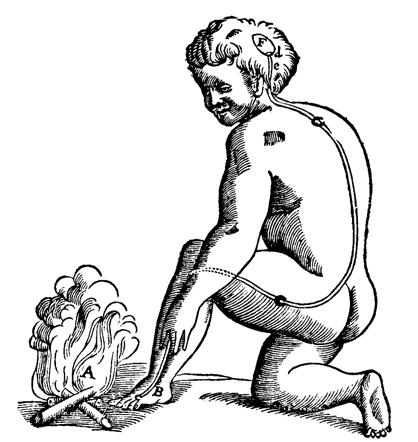
\includegraphics[width=0.5\textwidth]{descartes-reflex.JPG}
\centering
\caption{Illustration of Descartes' pain pathway from the Treatise of Man \protect\cite{descartes-wikipedia}}
\label{fig:descarte}
\end{figure}

Descartes' description was the first instance where the experience of pain was considered from a mechanistic perspective. The pain percept was for the first time framed as a physical system that could be understood and potentially treated.

\subsection{Theories of Pain}
 
The concept of a pain specific pathway was first put forward by Charles Bell where he proposed that the brain is a heterogeneous structure, and that nerves are a mix of heterogeneous neurons that became bundled to facilitate anatomical distribution \cite{Bell1868}. Evidence soon followed with the discovery of specific touch receptors and the demonstration that resection of posterior spinal tracts in animals by Schiff and Woroschiloff isolated innocuous touch from pain and temperature conductance (anterolateral tract) \cite{Dallenbach1939}. Von Frey demonstrated distinct receptive fields that respond to pressure that triggered tactile, warm, cold and pain. Sherrington further developed the specificity theory by coining the term “nocicipient” and unified attributes of intensity theory and specificity theory \cite{Casey1982}.

The classic pattern theory on the other hand, as first proposed by John Paul Nafe in the 1929 paper “A quantitative theory of feelings”\cite{Nafe1929}, postulates that the pain is not mediated by a separate nervous system or specialized receptors, but rather by units of undifferentiated afferent nervous impulses that only vary in their numbers, spatial and temporal relationships, including impulse frequency, duration, and density of nerve unit activations. The pattern theory postulates that all bodily sensations are a result of the brain's interpretation of nervous impulses. The discovery of high threshold mechanoreceptors and unmyelinated nociceptors however discredited the pattern theory and gave further credence to the theory of specificity. 

The gate-control theory \cite{Melzack1965a} (Figure \ref{fig:gate-theory}), which forms the basis of modern theory of pain, postulates that the cells of the substantia gelatinosa selectively inhibit signal transmission from primary afferent to the central transmission cells in the spinal dorsal horn that relays touch or pain sensations. The transmission control depends on the large and small diameter primary afferents, where large fibers inhibit, while small fibers facilitate the transmission. The gate-control theory reconciles the two previously divergent specificity and pattern theories of pain.

 \begin{figure}[ht]
 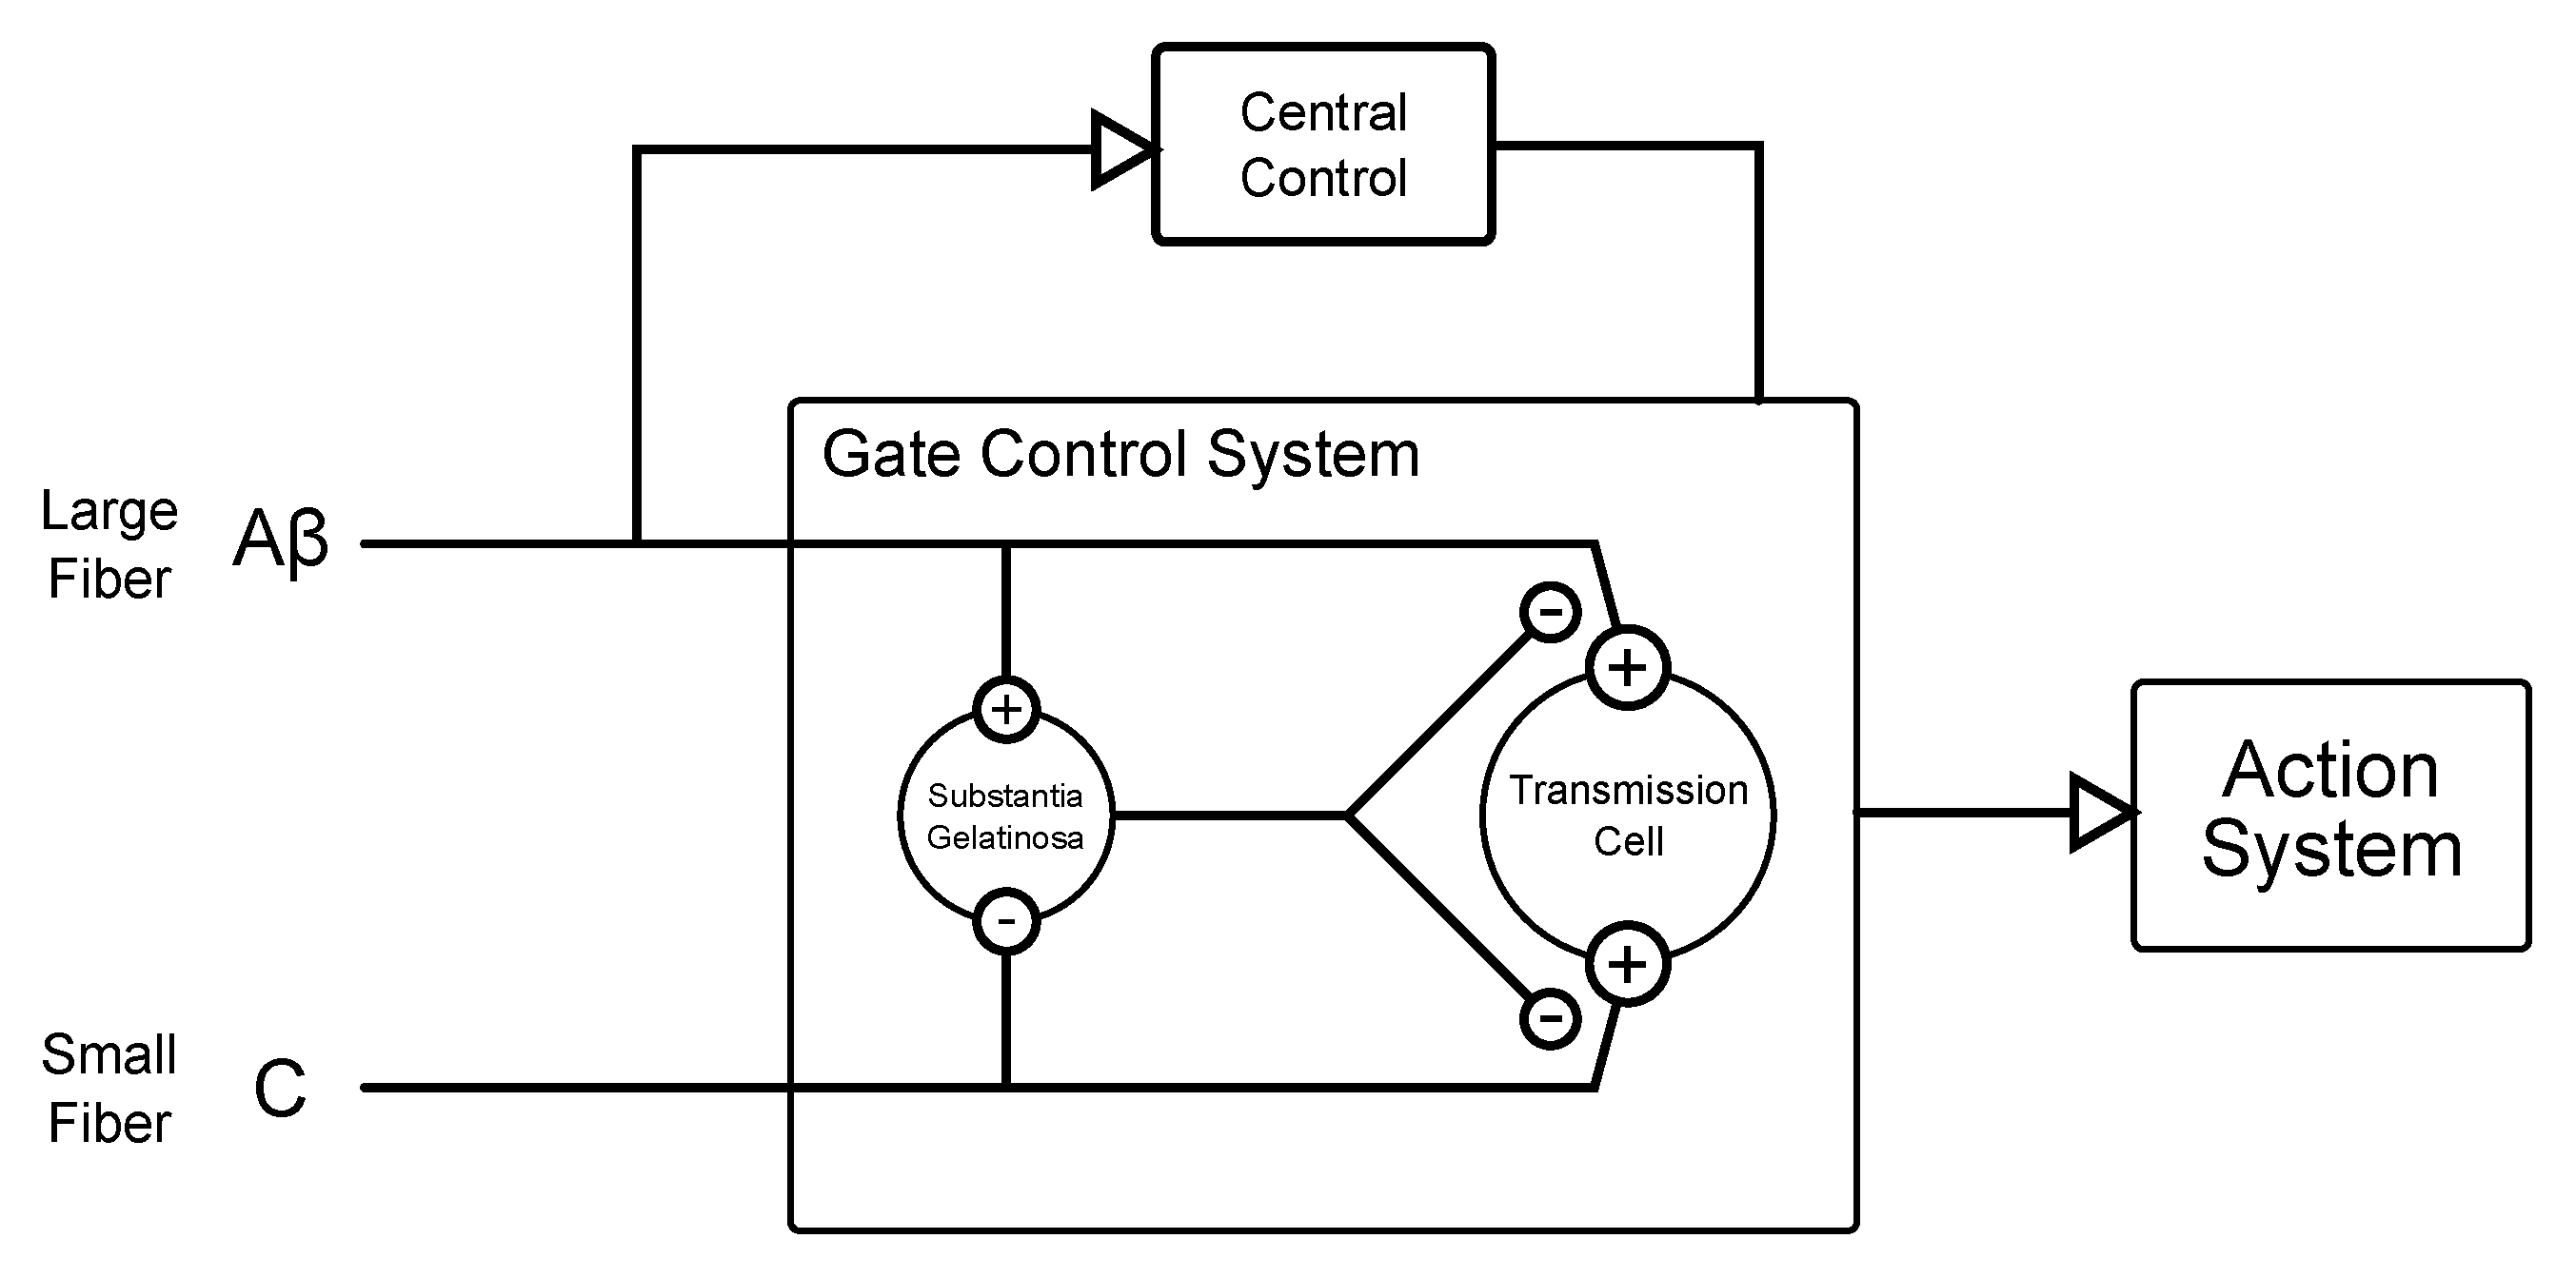
\includegraphics[width=\textwidth]{gate-control-diagram.pdf}
 \centering
 \caption{Melzack's gate control theory diagram. Modified from \protect\cite{Melzack1965a}}
 \label{fig:gate-theory} 
 \end{figure}
 
An important contribution of the gate-control theory was to emphasize central nervous system mechanisms \cite{Melzack1999}, and the role of the dorsal horn in pain processing, and therefore reconciles the evidences of pain-specific primary afferent and with pattern theory. Contemporary views consider pain to be complex and multi-dimensional, where the processing of ascending nociceptive signals, in conjunction with descending modulatory pathways, shape the pain experience. Melzack and Casey further proposed that pain consists of sensory-discriminative, affective-motivational, and cognitive-evaluative components \cite{Melzack1968}. Specifically, the sensory-discriminative component consists of peripheral nociceptive afferents transmit to the spinal dorsal horn (laminae V), whereby nociceptive specific (NS) and wide-dynamic-range (WDR) neurons convergently process these primary afferents, and relay them to the thalamus, and subsequently the primary sensory cortex. A central concept, which was also introduced by Melzack, is the  neuromatrix theory of pain, which dictates that the pain experience is produced by a "neurosignature" pattern, that is generated from widely distributed neural network, which Melzack refers as the "body-self neuromatrix". \cite{Melzack1999}. The concept is now more commonly referred to as the "pain matrix" \cite{tracey2007a}. (See section \ref{section:neuromatrix})


\subsection{Pain Physiology}

\subsubsection{Peripheral Receptors}

\textit{Nociceptors}, the peripheral nociceptors respond to noxious stimuli. These receptors have free nerve endings, and can respond to thermal, mechanical, and/or chemical stimuli, such as physical trauma or heat/cold temperatures. These receptors broadly separate into two categories, differentiated by the fibre type. Acute nociceptors are associated with $A\delta$ fibres, which permit fast signal conductance (5 to 30 m/s) and trigger a prickly or sharp pain sensation; examples include needle prick other acute trauma. Dull pain is triggered by receptors that are associated with slow conducting C fibres ($<1$ m/s). $A\delta$ and C fibres can be co-activated in the presence of noxious stimuli. C-fibre nociceptors can be further differentiated into mechano-heat, silent, and polymodal subtypes. $A\delta$-fibre nociceptors can be divided into high-threshold mechano-heat, low-threshold mechano-heat, and noxious cold subtypes.

\subsubsection{Nociception in the spinal cord}

The peripheral nociception signals are conducted from the axonal endings of the nociception neurons, whose cell bodies are located in the spinal cord dorsal root gangions, to the dorsal horn of the spinal cord (\ref{fig:drg}). The $A\delta$ and C afferents project directly to lamina I of the dorsal horn. $A\delta$ afferents also directly project to lamina V. Lamina II, or the substantia gelatinosa, also receives inputs from C afferents, which indirectly synapse to lamina I neurons through interneurons. The dorsal horn also contains a dense layer of local interneurons in lamina III and IV, and receive input from innocuous somatosensory afferents at these layers. 

\begin{figure}[ht]
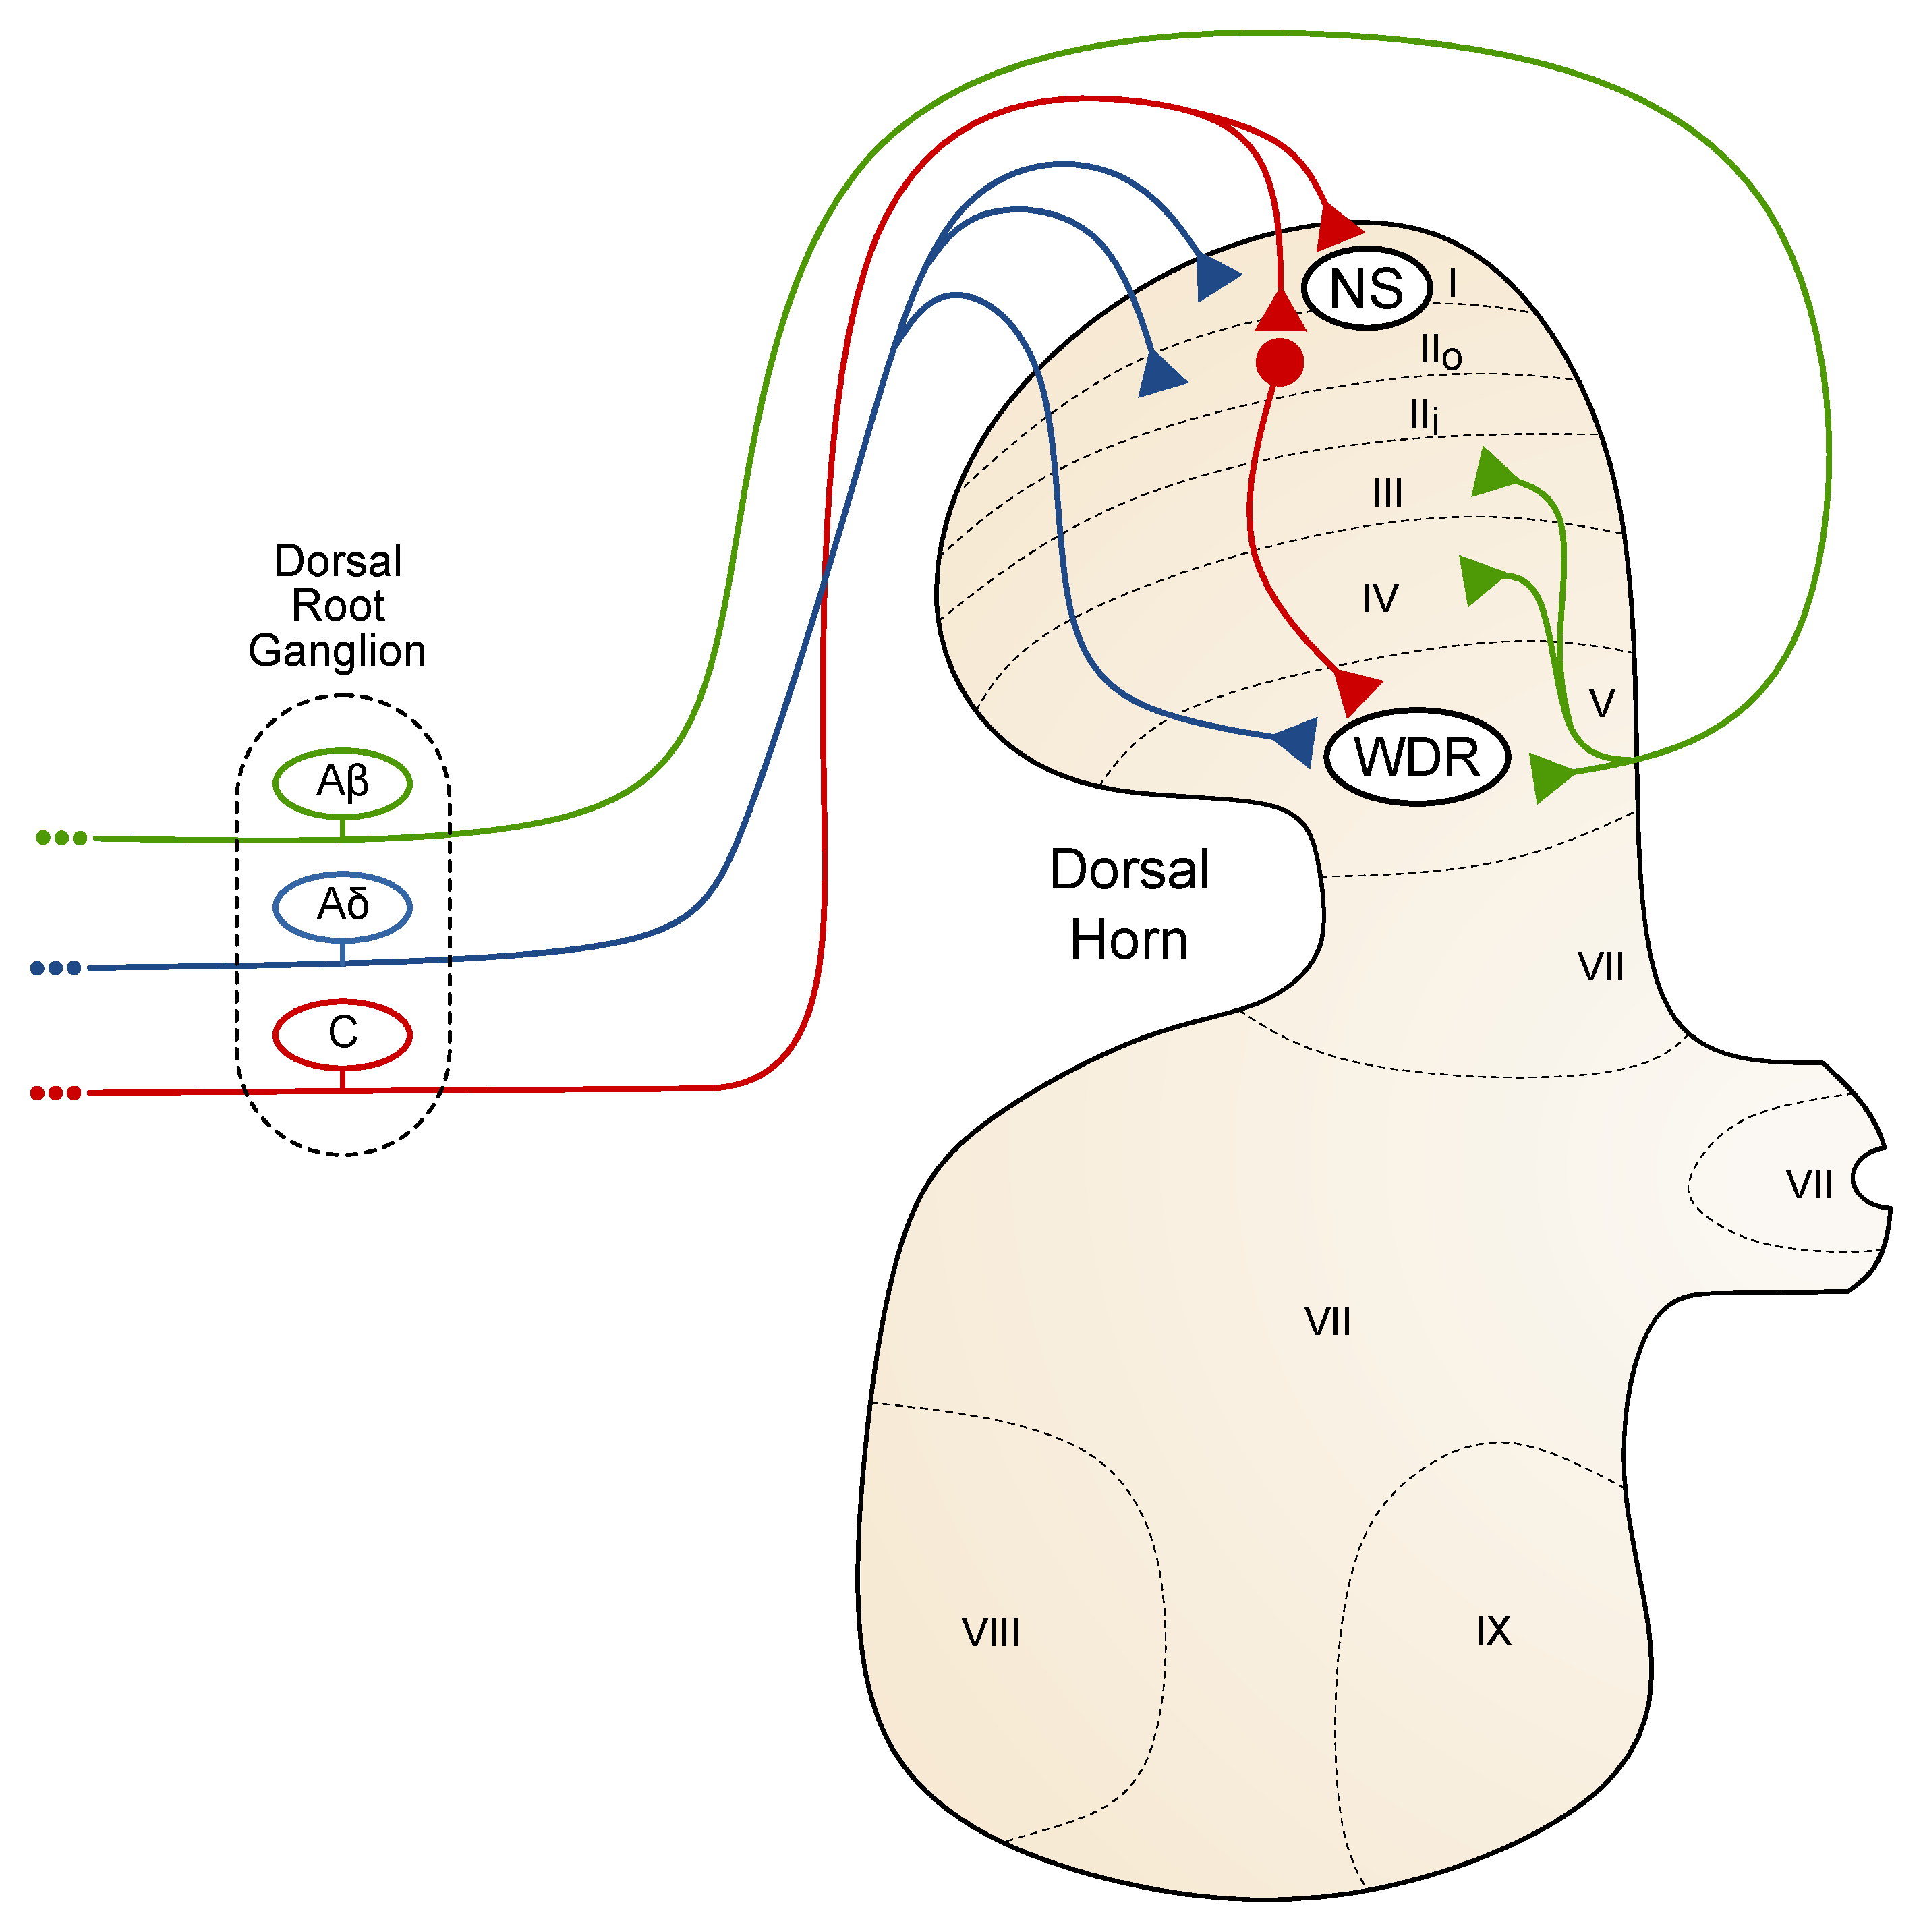
\includegraphics[width=0.8\textwidth]{dorsal-lamina.pdf}
\centering
\caption{The axonal projections of the fast conduction ($ A\delta$) and slow conducting (C) pain stimuli in the dorsal horn.}
\label{fig:drg}
\end{figure}
 
The interneurons in the dorsal horn plays an important part in somatosensory integration as the sensory afferent pass from peripheral into the central nervous system. For example, the wide dynamic range (WDR) neurons are found primarily in the spinal dorsal horn in lamina V-VI. These neurons respond to both innocuous and noxious stimuli, and are decidedly non-specific. They are found to sustain their impulse discharge during long durations of repetitive nociceptive stimulation, while nociceptive specific (NS) neurons showed a declined discharge rate within the same duration \cite{Coghill1993,Maixner1986}, thereby providing evidence that WDR neurons are responsive to prolonged nociceptive pain. 

In each spinal afferent level, the dorsal horn neurons project noceciptive signals to the brain via five distinct paths (Figure \ref{fig:pain-pathways}). Lamina I, V-VII axons crosses the mid-line to form the \textit{spinothalamic} tract that ascend in the contralateral anterolateral column of the spinal cord, and project to thalamic nuclei. Laminae VII and VIII neurons from the \textit{spinorecticular} tract ascend via the anterolateral quadrant of the spinal cord, without crossing the midline, to reach the reticular formation and thalamus. The \textit{spinomesencephalic} tract include axons from laminae I and V, and ascend in the anterolateral quadrant to the mesencephalic reticular formation, including the periaqueductual gray. The \textit{cervicothalamic} tract include only the white matters of the upper two cervical segments. It takes inputs from laminae III and IV, and projects to the thalamus via the medial lemniscus. The spinohypothalamic tract contains axons from laminae I, V, and VIII, and project to hypothalamic nuclei for autonomic functions. 

 \begin{figure}[ht]
 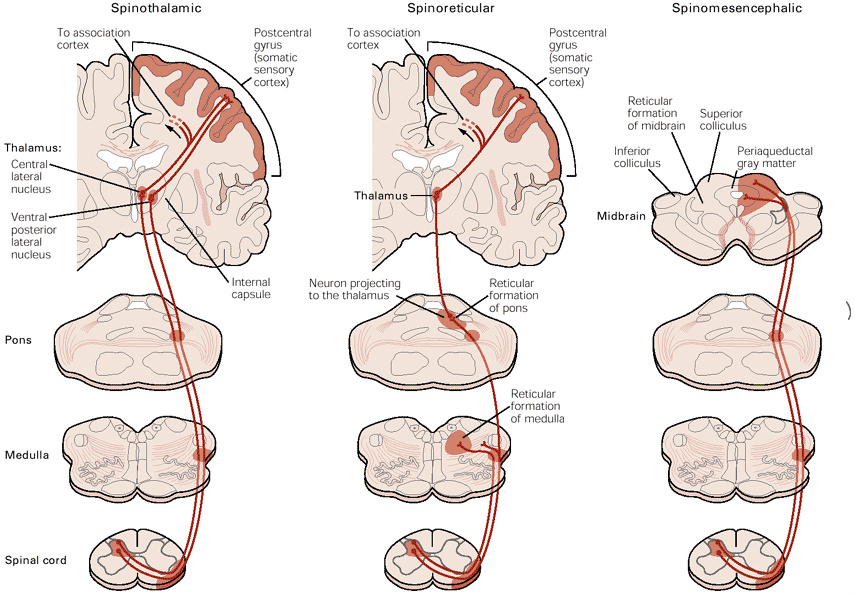
\includegraphics[width=\textwidth]{pain-pathways.jpg}
 \centering
 \caption{Afferent pain pathways \protect\cite{kandel2000principles}}
 \label{fig:pain-pathways}
 \end{figure}
 
 
\subsubsection{Thalamus}

Before reaching the neocortex, several important second order pain afferents arrive at the thalamus. The spinothalamic tracts subserving face and body sensory information terminate in several regions of the thalamus. A major termination site is the ventroposterior complex (VP, also known as ventrocaudal (Vc) nucleus), where ventroposterior-medial (VPM) nuclei and ventroposterior-lateral (VPL) nuclei are termination sites for the face and body respectively. The VP complex sends third-order afferents to the primary sensory cortex (S1). Thus, the VP representation is somatotopically organized with the face region in the medial aspect, and lower limbs towards the lateral aspect. The representation is retained in the cortical projection, where the S1 somatotopy is shown to have the face region towards the lateral surface of the S1 cortical strip, and lower limb towards the superior-medial aspect. 

Another spinothalamic termination site is the mediodorsal (MD) nucleus of the thalamus, where pain afferents of the spinothalamic tract that originated from dorsal horn lamina I layer synapse. The MD nucleus projects third order afferents to the anterior/middle cingulate cortex (ACC/MCC), which is shown to be prominent in the emotive/suffering cognitive aspect of pain.  

An important nucleus thought to be unique in humans is the ventromedial-posterior nucleus (VMpo)\cite{Willis2002,Craig2014}. It receives inputs primarily from dorsal horn lamina I, and can be considered to be contiguous with the basal ventral medial nucleus (VMb), that forms a relay for homeostatic afferents \cite{Craig2003}. The VMPo projects to the dorsal posterior insular cortex, which is thought to involve body interoception of pain.

\subsubsection{Cortical projections of pain}\label{section:neuromatrix}

Pain percept, defined as the subjective experience of pain, is thought to involve distributed regions of the brain, coined as the pain “neuromatrix”\cite{Melzack1999a}, or more commonly the "pain matrix". The regions are not functionally independent, but rather thought to be dynamically inter-related. 

 Important cortical regions involved in pain include anterior and middle cingulate cortices (ACC/MCC), insula, prefrontal cortex (PFC), thalamus, periaqueductal grey (PAG), secondary somatosensory cortex (SII) and motor cortex (M1). The role of these cortical regions in pain were studied in neuroimaging fMRI studies \cite{Apkarian2013c,Wager2013,Davis2012a}, which demonstrated consistent BOLD co-activations during noxious stimulation. (Figure \ref{fig:pain-matrix}).

 \begin{figure}[ht]
 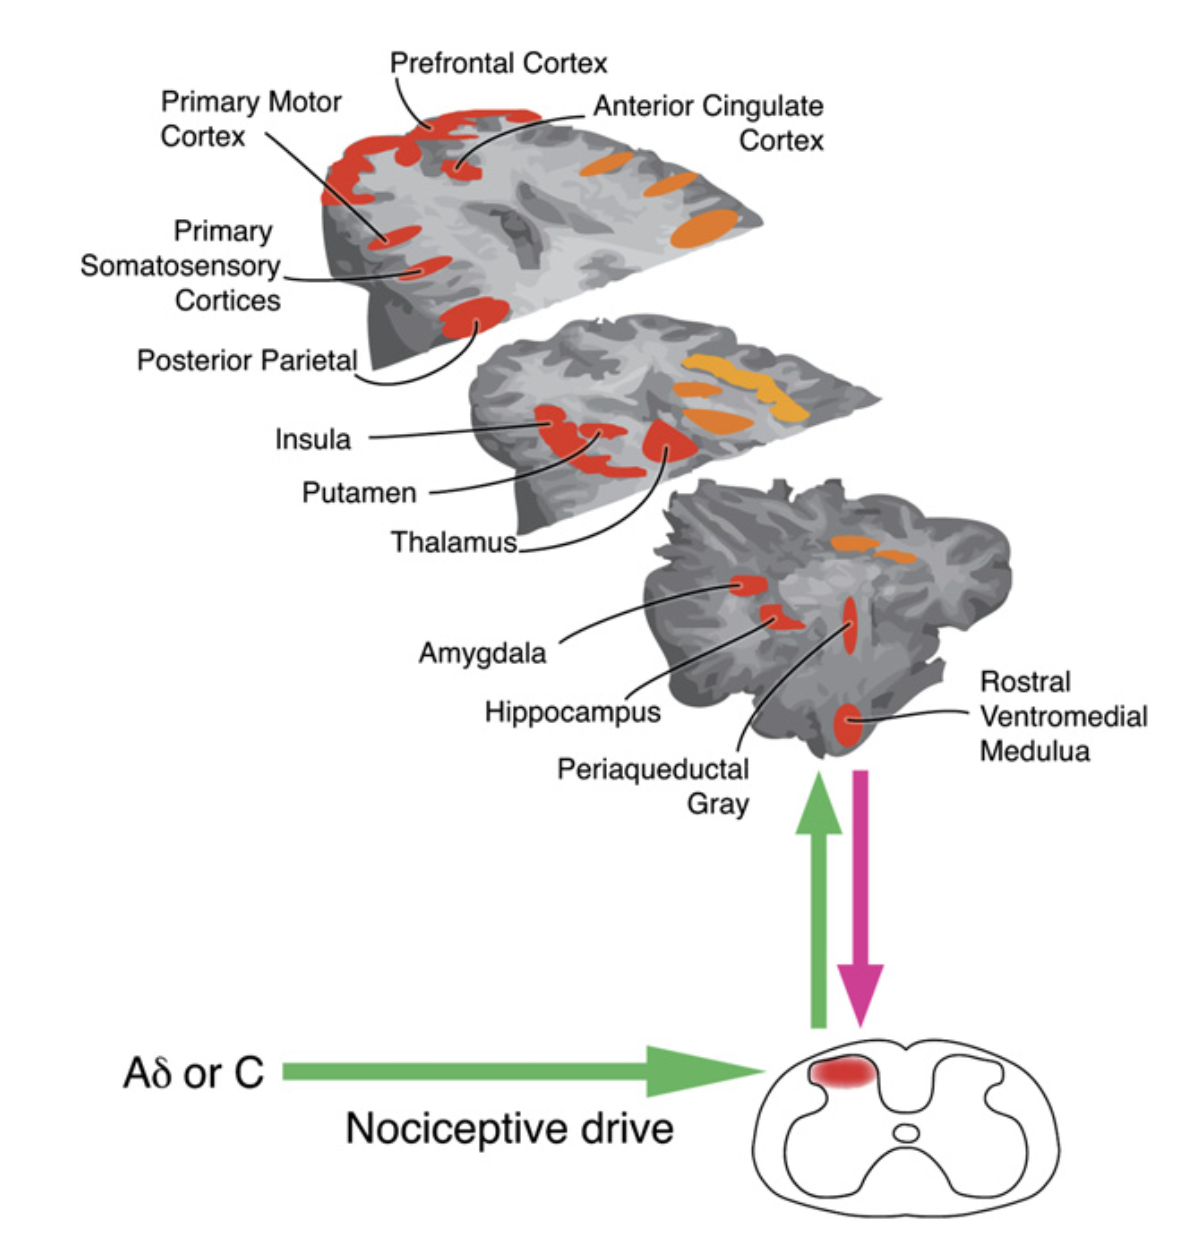
\includegraphics[width=0.8\textwidth]{pain-matrix.png}
 \centering
 \caption{ Cortical and sub-cortical regions of the pain matrix. \protect\cite{Tracey2007a}} 
 \label{fig:pain-matrix}
 \end{figure}
 
A recent study suggests that pain is correlated to the dynamically changing patterns of BOLD activities over time in the regions involved. Thus, the focus of the salient pain percept requires a switch away from the default mode network \cite{Kucyi2013}. The dynamic rhythms of activities that attune to and away from saliency, form a dynamic pain connectome \cite{Kucyi2015}. Chronic pain therefore demonstrated differential tuning of the default mode network and attention patterns of the brain due to their pathological activation of the pain matrix in the absence of detectable noxious stimuli \cite{Baliki2008,Legrain2009}.

\paragraph{Sensory-Discrimination}
Cortical regions associated with sensory-discriminative aspect of pain, such as the location and intensity of pain, include the S1 ana S2 cortices. The S1 cortex is responsible for the discrimination of fine-touch sensations. S1 receives inputs directly from VP thalamus. Nonetheless, S1 has not been consistently reported in acute pain studies, possibly due to the difficulty in detecting pain-related activations as there are relatively small number of nociceptive neurons within S1 \cite{bushnell1999pain}. S2, however, receives direct nociceptive input from VPI thalamus, and its BOLD activation is more consistently observed across pain fMRI studies \cite{Wager2013,Brodersen2012}. The posterior insula also receives direct nociceptive inputs from the VMpo thalamus \cite{Craig2003}, and shows strong functional and structural connectivity with S2 \cite{Wiech2014}. Therefore the insula, as well as S1, are believed to plays an important role in sensory-discrimination aspect of pain. 

\paragraph{Affective-Motivational}
The cortical regions that are involved in affective-motivational pain processing, including unpleasantness and flight response, involve both regions that receive direct projection from the medial thalamus, as well as indirection regions. The anterior cingulate cortex (ACC) receives direct cortical projection from the medial dorsal nucleus, while the anterior insula receives input from the VMpo thalamus. The amygdala is important for fight-flight reflex, and regions in the prefrontal cortices are believed to be related to the cognitive aspects of pain. These regions are demonstrated to correlate with the sensory-discriminative regions during the pain experience, but can be disassociated for example in pain empathy \cite{Singer2004}. The unpleasantness of pain has been thought to be a motivational force \cite{Auvray2010}, that biases actions towards avoidance. There is evidence that the motor cortex, which is involved in action planning, and the ACC/MCC are activated during pain \cite{Parker2016,Burns2016,Erpelding2013}. The cortical excitability of the motor cortex is also shown to be altered in chronic pain \cite{Parker2016}. The motivational system is also involved in pain-reward and involves the ACC, lateral orbitofrontal cortex (OFC), and the prefrontal cortex (PFC, both ventromedial and anterior aspects) \cite{Navratilova2015}. The nucleus accumbens (NAc) BOLD activity correlated with anticipation of pain relief \cite{Baliki2010}. The reward/motivational circuitry is thought to be disrupted in chronic pain, and such disruption is related to the emotional and cognitive deficits in chronic pain sufferers.

\paragraph{Default mode network}
The default mode network (DMN) are regions of the brain, including the cingulate cortex, which show highly correlative BOLD activations in fMRI during wakeful rest \cite{Greicius2003,Raichle2015}. The core regions associated with the default network are ventral medial prefrontal cortex (vmPFC), posterior cingulate, inferior parietal, lateral temporal cortex, dorsal medial prefrontal cortex (dMPFC) and hippocampal formation. Regions such as vmPFC, dMPFC and the anterior cingulate overlap with the affective-motivational pain matrix, and are found to be disrupted in DMN in chronic pain \cite{Baliki2008}. Pain related DMN deactivation have been found to be attenuated  in mind wandering away from pain, and may reflect antinociceptive processes \cite{Kucyi2013}, and that the DMN may undergo functional reorganization under chronic pain \cite{Baliki2014}. 

\paragraph{Insula}

The insula is an important neuroanatomical structure that has been implicated in both acute \cite{Lorenz2005,Starr2009} and chronic pain \cite{May2008,Jensen2016}. Anatomically it is subdivided into anterior and posterior components by the central insular sulcus. It can be further identified by its gyral features, consisting of 5 major gyri: anterior, middle and posterior short gyri in the anterior insula, and anterior long, posterior long gyri of the posterior insula. These gyri are not found consistently in the general population, but rather show individual variability \cite{Rosen2015}. Craig postulates that the insula is a key region for homeostasis and interoception \cite{Craig2003b}, and is necessary for pain discriminative sensations via VMpo projections in the middle insula in humans \cite{Craig2003a}. 

There is a recent debate pertaining the dorsal posterior insula as the "pain cortex" \cite{Segerdahl2015a}. Segerdahl et al. suggested that there is strong coupling between absolute cerebral blood flow and tonic pain intensity, and utilized arterial spin-labelling to quantify cortical activation in response to pain stimulation. The contralateral dorsal posterior insula emerged as the only cortical region with significant correlation. Tract tracing studies in monkeys has previously revealed pain-modality specific anatomy in the subregion of the dorsal posterior insula \cite{Craig2014}, and the study suggested that this is a strong supportive finding of a homologue region in humans. Critics of this finding raised issues with the low number of subjects, long sampling duration and the incompatibility of this interpretation with long standing bodies of neuroimaging and neurophysiological literature \cite{Davis2015}. 

\subsection{Chronic Pain}

Chronic pain is pain that persists past the healing phase following an injury \cite{Apkarian2009,Merskey2012}. It is more commonly defined as pain symptoms that persist longer than a fixed duration, most commonly 3 to 6 months. Other factors to consider include psychosocial factors such as emotional and functional stress in addition to pain severity \cite{Treede2015}. The new ICD-11 revision of chronic pain classification include a new category for chronic primary pain. It is defined as "pain in one or more anatomical regions that persists or recurs for longer than 3 months, and is associated with significant emotional stress or significant functional disability" \cite{Treede2015}. It includes chronic pain conditions where the etiology is unknown. Conditions such as fibromyalgia, and irritable bowel syndrome fall under this category. Chronic pain conditions are considered to a type of maladaptive pain, whereby the pain response no longer serves its role in protecting the body from harm, but rather contributes negatively to the normal functions of life \cite{May2008}. 


\subsubsection{Neuropathic Pain}

Neuropathic pain is a type of chronic pain, defined as "pain caused by a lesion or disease of the somatosensory nervous system"\cite{Merskey2012}. The pain experience may be constant or paroxysmal, related to a stimulus (evoked) or spontaneous. Animal models of neuropathic pain suggest that peripheral and spinal circuitry responsible for the transmission of nociception are altered under pathological conditions. The nervous system is believed to be altered by maladaptive plasticity following a nervous system insult thereby resulting in sustained neuropathic pain.

The maladaptive mechanism responsible for neuropathic pain may manifest in any stage of the nociceptive transmission, processing, and descending modulatory circuitry. 
Noxious signal arises in the periphery, and undergoes signal transformation in the periphery and spinal ganglions, and is then subsequently processed as the pain percept in the neocortex. The pain percept is also modulated by emotional and cognitive factors, which triggers downstream modulation that ultimately affects the nociceptive signal transformation. 

Peripheral neuropathic pain often occurs after lesion to the peripheral nervous system, and can be caused by physical trauma and infections. Central neuropathic pain is caused primarily by lesions in the central nervous system, including spinal cord injury, lesions relatting to multiple sclerosis or tumours. 


\paragraph{Peripheral Sensitization}

Peripheral neuropathic pains can arise when there are disruptions in peripheral signal transmission. The disruption can be a result of injury to the first order peripheral afferent neurons, which result in increased sensitivity to stimuli and via ectopic action potentials. Changes in peripheral neurotropic factors as a result of an injury can cause increased membrane excitability or spurious sprouting of the synaptic terminals in the dorsal horn of the spinal cord. Additionally, maladaptive changes may occur in the secondary sensory neurons and interneurons in the dorsal-horn laminae that amplifies or reroutes the noxious signals \cite{Elmes2004}.

\paragraph{Central Sensitization}

Neuropathic pain can also arise from changes in the central neuroaxis. Trauma and other disruptions to the spinal pathways can affect noxious signal transmission. White matter pathways within the brain may also become damaged by conditions such as trauma, infections, and multiple sclerosis. It is believed that injury to white matter fibers can affect action potential conduction between cortical and subcortical structures. This may give rise or contribute to neuropathic pain \cite{Geha2008}.

 The utilization of magnetic resonance imaging (MRI), coupled with novel imaging modalities such as functional MRI (fMRI) and diffusion MRI (dMRI), have been instrumental in our understanding of pain, permitting both \textit{in vivo} measures of brain activity during pain (functional studies) \cite{Davis2006}, as well as assessment of changes to the brain microstructure \cite{Hodaie2009a,Chen2015c}.
 
 Neuropathic and acute nociceptive pain have a high degree of overlap in brain activations \cite{Moisset2007}, therefore differentiating between neuropathic and acute pain from neuroimaging continue to be an active area of research. Brain regions that are involved in the somatosensation of pain process are involved in both acute and chronic pain. These regions include the posterior insula, lateral thalamus and dorsal striatum. In chronic pain conditions however, there is increased activation in the anterior insula, ventral striatum, orbital frontal cortex and dorsal lateral prefrontal cortex \cite{Lorenz2005}. In chronic back pain, diffusion changes in fractional anisotropy was correlated with medial prefrontal cortex and nucleus accumbens connectivity in pain recovery, but not when the pain persistented \cite{Mansour2013}. Evidence also suggest that back pain chronification seem to increase activation in the emotional regions (amygada and medial prefrontal cortex) of the brain, and transition away from sensory region activations \cite{Hashmi2013}. A shift in forebrain activities is observed in neuropathic versus acute pain, abnormal activities in anterior cingulate cortex and prefrontal cortex is commonly observed in these studies \cite{Davis2006}. 
 
 Advances in modern machine learning methods led to their uses in attempting to improve neuropathic pain classification and diagnosis. Modern approaches combines cross-modal and additional analytical features, and can involve fMRI, diffusion imaging, as well as functional and/or structural connectivity. Machine learning in the form of multivariate pattern analysis to classify individuals with chronic back pain from normal controls, and achieve 92\% accuracy \cite{Callan2014}. Other studies in chronic pelvic pain using linear support vector machine was able to achieve 73\% accuracy \cite{Bagarinao2014}. Differentiating neuropathic and acute pain however is more difficult. Functional connectivity based classification on differentiating fibromyalgia, rheumatoid arthritis and controls was able to achieve a diagnositc accuracy of 69\%, and classification accuracy of 78\% \cite{Sundermann2014}.    
 
 
\section{Trigeminal Neuralgia}

Trigeminal neuralgia (TN) is a chronic neuropathic facial pain disorder, that commonly affects one or more branches of the trigeminal nerve. TN symptoms involve paroxysmal, shock-like pain condition affecting one or more of the three facial sensory nerve branches. The pain episodes can be unpredictable, as the length of episodes can range from months to years \cite{Katusic1990}. Patients often describe its symptom as the most painful experience a human can undergo. Its physical and emotional disturbances can be severely disabling. 

This disorder has been documented as early as the first century AD, the clinical recognition of the disorder was by Nicolaus Andre in 1756, and by John Fothergill in 1776 \cite{Katusic1990}. In the three hundred years that followed, the etiology of TN is still not understood. The modern understanding of the vascular compression of the trigeminal nerve root was first proposed by Janetta \cite{Jannetta1967}, where he elucidated that TN is a “nerve entrapment disorder” and that it may be a “consequence of ageing … by arterialsclerotic elongation of the cerebrovasculature”.

Modern pain literature continues to update the exact diagnostic definition of TN. The Burchiel classification scheme divides facial pain into 5 major subtypes \cite{Burchiel2003,Eller2005}: idiopathic (without apparent cause), trigeminal injury, symptomatic, postherpetic, and atypical facial pain. Idiopathic TN has 2 sub-types: 1) TN type 1, also referred to as classic TN, where the patient experiences greater episodic pain greater than 50\% of the time; 2) TN type 2, where constant pain occurs greater than 50\% of the time. Trigeminal injury can be unintentional: which can be due to facial trauma, surgery to the oral cavity; this type of pain would involve persistent and burning pain to the affected areas; and is termed trigeminal neuropathic pain. The injury can also be intentional, due to interventions such as rhizotomy or gangliolysis; these result in numbness and loss of sensation of the face and are termed trigeminal deafferentation pain. Symptomatic TN, also termed MS-TN, is due to trigeminal nerve injury relating to multiple sclerosis related central white matter inflammation. Postherpetic TN is pain resulting from the infection of the herpes zoster virus, and can involve burning pain and deafferentation. In this classification, the definition of atypical facial pain is reserved for somatoform pain disorder that can be of psychosomatic origin, although some literature can also include constant pain in the face into this classification. This is in contrast with the common clinical definition, where atypical facial pain is used for the definition of trigeminal pain whose symptomatology deviates from classic TN.

The current The International Classification of Headache Disorders ICHD-3 Beta \cite{Society2013} classifies TN into classic TN, and painful trigeminal neuropathy. 
Classic TN's diagnostic criteria requires pain characteristics of: at least 3 attacks of unilateral facial pain; occurring in one or more trigeminal branches, with no radiation beyond the trigeminal distribution; severe intensity; electric shock-like, shooting, stabbing or sharp in quality; and precipitated by innocuous stimulation to the affected side of the face; and no clinically evident neurological deficit. Classic TN is further divided into purely paroxysmal: recurrent attacks of unilateral facial pain with no persistent facial pain between attacks; and concomitant persistent: persistent facial pain of moderate intensity in the affected area. 
Painful trigeminal neuropathy, in contrast, is facial pain in one or more distributions of the trigeminal nerve caused by another disorder and indicative of neural damage. It can be further divided into categories relating to acute Herpes zoster, post-herpetic trigeminal neuropathy, multiple-sclerosis, space-occupying lesion, and other disorders.

There is also a definition \cite{Zakrzewska2016} that attempts to address the lack of symptomatic TN classification in ICHD-3 by classifying TN into idiopathic, classic TN, caused by vascular compression of the trigeminal nerve root and secondary TN, as the consequence of a major neurological disease such as MS. 

\subsection{Trigeminal Anatomy}

The trigeminal nerve, or the fifth cranial nerve (CN V) is the primary afferent for both facial somatosensation and pain (\ref{fig:trig-branches}). It consists of, from superior to inferior, the ophthalmic (V1), maxillary (V2) and mandibular (V3) branches. The distribution of the branches consists of both motor and sensory components. The motor branch of CN V activates the muscles responsible for mastication, as well as tensor tympani, tensor velipalatini, mylohyoid and anterior belly of the digastric. 

 \begin{figure}[ht]
 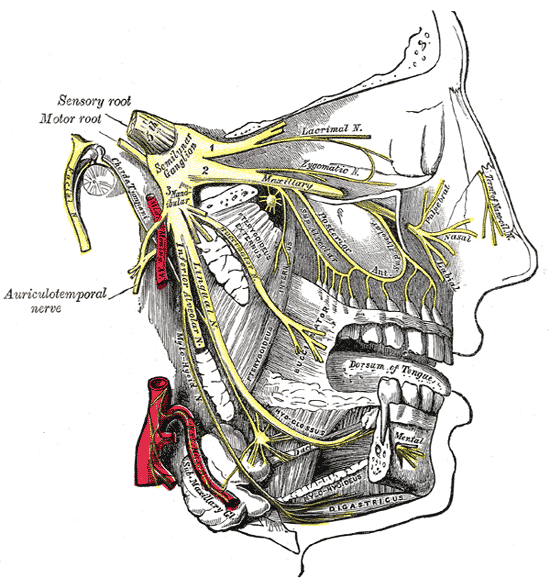
\includegraphics[width=120mm]{trig-branches.png}
 \centering
 \caption{Anatomy of the trigeminal nerve branches. \protect\cite{gray1918anatomy}} 
 \label{fig:trig-branches} 
 \end{figure}
 
The sensory afferents include the myelinated A and unmyelinated C-fibers that originate from the subcutaneous sensory receptors responsible for mechano- and temperature pain, fine touch and vibration, such as the Messner's, Pacinian and Ruffini corpuscles. 

The V1 branch provides the sensory innervation to the superior aspects of the face and cranium, including forehead, upper eyelids, eyeball, frontal sinus, lacrimal gland, and dura of the anterior cranial fossa. It further divides into lacrimal, frontal, and nasociliary nerve branches. The lacrimal branch supplies the lacrimal gland; the frontal contains smaller branches that innervate the skin of the medial forehead, upper eyelid, and parts of the frontal sinus; the nasociliary branch innervate various parts of the eye, and mucous membrane of the anterior nasal septum, anterior portion of the lateral nasal wall, and the skin on the tip of the nose. V1 exits the skullbase through the superior orbital fissure.  

The V2 provides innervation to the temple, cheek, lateral aspects of the nose, and lower eyelids via the zygomaticofacial and zygomaticotemporal branches. It also innervates upper oral cavity. It exits the skull through the foramen rotundum. 

V3 contains sensory and motor branches. It innervates skins of the jaw, areas above the ear, lips, gum, and teeth. The V3 division carries the mastication efferent to the four muscles recruited for mastications: the masseter, temporal, medial and lateral pterygoids. The tensor tympani also receives some CN V innervation, but it is primarily innervated by the facial nerve.  It is thought that CNV innervation is important in dampening the sound of chewing. V3 exits the skull through foramen ovale. 

The afferent branches converge and form the trigeminal root gangion (TRG) (also known as Gasserian, or semilunar ganglion), which then forms the trunk or cisternal component of CN V. The TRG contains all the trigeminal sensory cell bodies. It situates in the Meckel's cave, in the middle cranial fossa. It is anatomically organized with respect to the trigeminal branches, with V1 situated in medial anterior, V2 in caudal lateral, and V3 in the middle.

The extension of the posterior aspect of the TRG forms the trigeminal nerve body, with both sensory and motor roots. The nerve body straddles the TRG and the trigeminal nucleus, by crossing the pontine cistern. The portion of the sensory nerve that enters the pons is termed the trigeminal root entry zone (REZ). The cistern trigeminal sensory nerve, similar to other peripheral nerves, is myelinated by Schwann cells. The myelin cell type transitions to oligodendrocyte myelinations in the CNS as it enters the pons. The CNS myelin can be several millimetres beyond the surface of the pons, before it gives away to the transition area, termed root entry zone, or Obersteiner-Redlich zone \cite{Peker2006}. Study in 100 CN V samples from 50 cadavers showed that cisternal CN V length ranges from 8-15 mm; the transition zone length is shorter on the medial aspect (0.1-2.5 mm) than the lateral aspect (0.17-6.75 mm). The transition zone can be up to 25\% of the nerve length \cite{Peker2006}. 

 \begin{figure}[ht]
 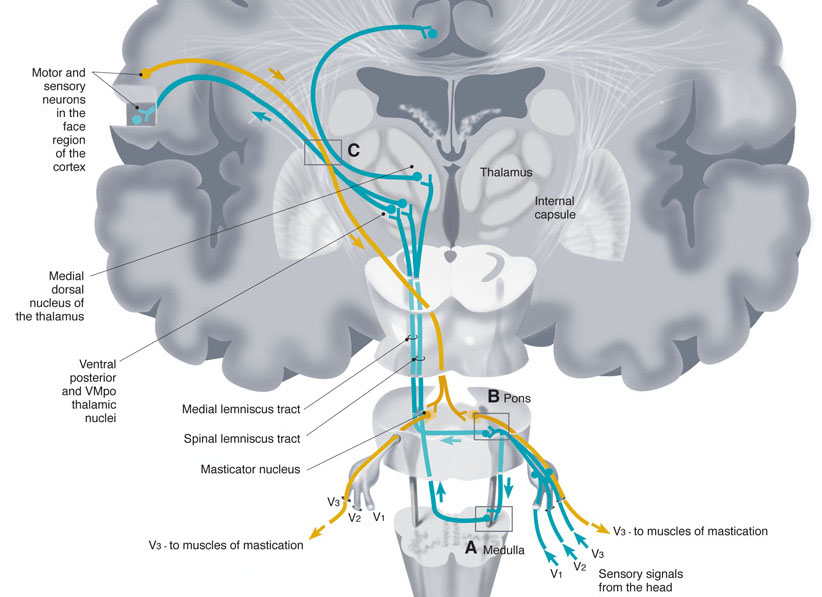
\includegraphics[width=\textwidth]{trig-pathway-wilson.jpg}
 \centering
 \caption{Overview of the trigeminal afferent pathways \protect\cite{wilson2010cranial}}
 \label{fig:trig-pathway}
 \end{figure}
 
CN V passes into the pons (\ref{fig:trig-pathway}), through the transverse pontine fibers and enters the tegmentum of the pontine brainstem. It then curve towards the medial line before synapses onto the trigeminal nucleus in the basis of the pontine brainstem. The trigeminal nucleus is divided, from superior to inferior, into the mesencephalic, main sensory, and spinal nuclei. The spinal nucleus can be further divided into pars oralis, pars interpolaris and pars caudalis. 

The mesencephalic nucleus is responsible for proprioception, while the spinal trigeminal nucleus receives ipsilateral pain and temperature afferents not only from CN V, but also from CN VII, CN IX and CN X. Pars oralis transmits fine tactile sensations from the oralfacial region, pars interpolaris is associated with dental pain, while pars caudalis is responsible for nociception and heat from the head. 

The main sensory nucleus receives discriminative somatosensation from the oralfacial region, and along with the spinal trigeminal nucleus fibers, project to the contralateral ventral caudal nucleus (VC) of thalamus by decussating at various levels of the pons via the anterior trigeminothalamic tract. A separate branch responsible for oral cavity, however, projects to the ipsilateral VC via the dorsal trigeminothalamic tract.  

The VC thalamus projects to the primary sensory (S1) and secondary sensory (S2) cortical regions of the neocortex, thereby completing the afferent sensory projections of CN V. 



\subsection{Pathophysiology}

Classic TN is believed to be caused by neurovascular compression (NVC) of the CN V at its root entry zone (REZ) by the surrounding vasculature, where the nerve interfaces with the pons. An aberrant loop of artery and less commonly a vein is seen in 80-90\% of the cases of TN compressing the nerve \cite{Love2001,McLaughlin1999}. This can also be observed in conventional MR imaging \cite{Borges2010}. The superior cerebellar artery is responsible for most of the NVC (60-90\%), followed by the anterior inferior cerebellar artery (AICA) and basilar arteries \cite{Lutz2011}. There is a slight lateral prevalence, with right-sided TN occurring in  in 60\% of the cases, and in rare cases may be related to asymmetries of the foramen rotundum and foramen ovale \cite{Toda2009}.  Other types of compression may also cause TN; these can be in the forms of vestibular schwannomas, meningiomas, epidermoid cysts, and other cerebellopontine angle tumours, arteriovenous malformations and saccular aneurysms \cite{Haller2016,Love2001}. However NVC cannot be assumed to be directly causal of TN, since observation of vascular compression does not necessarily result in the clinical expression of pain \cite{Desouza2013,Hodaie2013}. In approximately 10-15\% of cases where TN occurs with no observable vascular compression \cite{Revuelta-Gutierrez2006,Maarbjerg2015}.


Janetta \cite{Jannetta1967} proposed that NVC leads to focal demyelination of the trigeminal sensory root axons, and causes ephaptic nerve conductances that cause neuralgia. Ultrastructural examinations \cite{Love1998} of tissue samples obtained from CN V rhizotomy specimens showed oligodendrocyte demyelination at the site of root transition zone. Adjacent to the site of compression-related focal demyelination, thinly myelinated sheaths that encapsulate a number of demyelinated axons could be observed, suggesting aberrant remyelination. It is therefore plausible that NCV disrupts the central myelin. The region of disruption may include the peripheral-central myelin transition zone, and extending into central myelin regions.The TRG is also postulated to be responsible for neuralgia \cite{Rappaport1994}. It is believed that ganglionic ectopic autonomic firing can be triggered by mechanical disturbances as a result of nerve compression. Additionally, ganglionic cross aftercharge may occur as a result of repeated stimulations in the nerve injury site, which ignites surrounding neurons. Histological findings by Devor et al. support the ignition hypothesis \cite{Devor2002a}, where demyelinated axons are shown to be in close apposition without intervening glia.  

\subsection{Treatment and outcomes}

The initial mode of treatment of TN consists in pharmacotherapy, primarily using anticonvulsant medication such as carbamazepine. While there is an initial, very good response to medical treatment, eventually nearly 50\% of patients will fail medical therapy, either due to side effects, or requirements of a progressive increase in dose \cite{Rappaport1994}. Multiple surgical treatments are available, from more central procedures addressing NVC to peripheral procedures such as neurectomy. The procedure that provides the greatest likelihood of pain relief is microvascular decompression (MVD) \cite{Lovely1997,Hodaie2013}, where the nerve is decompressed from the offending vascular structure through the placement of a piece of Teflon\textcopyright gauze. This is thought to dampen the pulsations of the artery on the nerve. MVD can result in 90\% pain relief immediately after surgery \cite{Zakrzewska2005}, and a long-term success rate of 70\% at 10 years \cite{Barker1996}.
Partial sensory rhizotomy (PSR) can also be performed, where the offending CN V branch is severed, with a response rate of 88-70\% \cite{Young1993,Zakrzewska2005}. 

Intervention can also be non-invasive, in the form of Gamma Knife radiosurgery (GKRS) \cite{Hodaie2012g}. The Perfexion GK system focuses gamma radiation from 192 cobalt-60 ($^{60}$Co) sources onto specific targets along the trigeminal nerve. The target is either on the cisternal segment of CN V or just outside of the REZ \cite{Daugherty2015}. Proximal targets correlate with longer pain relief, but also higher chance of facial numbness\cite{Xu2014}. The procedure requires a stereotactic frame, and a dose of 70-90 Gy delivered to the nerve. The effect is delayed and pain relief can be experienced in 4-6 weeks post-radiosurgery. GKRS treatments result in 75\% initial pain relief \cite{Tuleasca2015,Kondziolka2010}, about 50-80\% remain pain-free at 1 year, 45-65\% 2 years and 30-40\% 3 years after surgery \cite{Kondziolka2010,Sheehan2005}. More favourable treatment outcomes were related to no other accompanying symptoms, no prior surgery and shorter term pain history of fewer than three years.

\subsection{Neuroimaging of Trigeminal Neuralgia}

Neuroimaging of the TN has been challenging, due to the small diameter of the CN V and since the contrast of the CNS trigeminal pathways is difficult to distinguish from the surrounding on conventional MRI \cite{Borges2010}. In conventional MRI, the brainstem nerve segment can only be deduced from its surrounding structures \cite{Casselman2008}. Sequences that can visualize myelinated structures are chosen, these include T2-weighted MRI  sequences such as FIESTA and CISS. Manual segmentation of T1 and T2 MRI requires great effort, with mixed results \cite{Miller2008a}. Diffusion MRI provided fiber orientation, and early attempts to segment the trigeminal system showed promise \cite{Upadhyay2008,Habas2007f}. Additionally, DTI showed strong ability to visualize spatial relationships in white matter anatomy, for example in delineating fornix sub-regions \cite{Chen2015c}, and in visualizing the distortion of CN VII/VIII by vestibular schwannomas \cite{Chen2011b}.  

Application of tractography permitted visual reconstructions of human cranial nerves in vivo \cite{Hodaie2010}. Cisternal CN V could be reliably delineated with Gaussian tensors with just 25 MR gradient directions. This permitted high fidelity visualization and targeted characterization of CN V diffusivity in TN, demonstrating significant reduction in fractional anisotropy (FA) post-surgery at the site of the GK target \cite{Hodaie2009a}. Study of CN V diffusivity in conjunction with deep white matter using TBSS, again revealed reduced FA on the affected CN V, with also bilateral increased in radial, axial, and mean diffusivity. Disruptions were also found in the cognitive-affective, attention, and motor regions of the cortex, consistent with cortical patterns in chronic pain \cite{Desouza2013}. Lowered FA was reported in multiple TN studies \cite{Herweh2007, Lutz2011}. Study in temporomandibular disorder (TMD) showed a bilateral reduction in CN V FA compared to controls, with the FA of the affected side significantly inverse-correlates with pain duration \cite{Moayedi2012}, thereby demonstrating that CN V FA is related to nociception. The TMD study also revealed similar cognitive and motor disruption, and internal capsule FA significantly inverse-correlated with pain intensity. 
\section{Multiple Sclerosis}
This chapter will review multiple sclerosis (MS) as a disorder, given the importance of MS-related TN is an independent TN subtype. MS is a chronic autoimmune demyelination disease of the central nervous system. It is a progressive disease characterized by wide-spread lesions, or plaques, within the brain, spinal cord, and optic nerve. Its pathogenesis is related to the focal inflammation and damage of the central myelin, where the disruptions of the myelin sheath negatively affect signal transduction of the central white-matter, and thereby result in severe disability. MS symptoms can include cognitive deficits, fatigue, depression, motor weakness affecting the upper and lower extremities and neuropathic pain. Currently there is no cure for MS. An estimated 2,300,000 people world wide are affected by MS, and 50\% of the patients will require motor assistance 15 years after disease onset \cite{Goldenberg2012}. The course of MS can be highly variable due to the distinct plaque distribution pattern in each individual, and therefor MS is difficult to diagnose and treat.

MS is divided into four major clinical groups: 1) Relapsing-remitting (RRMS), 2) Secondary progressive (SPMS), 3) Primary-progressive (PPMS), and 4) Progressive-relapsing (PRMS). RRMS is the most common form of MS, affecting about 85\% of the people with MS. It is characterized by sudden relapse (major flare-up) of symptoms, followed by periods of remission where symptoms disappear. SPMS may develop in some RRMS patients, where the symptoms worsen or level off. PPMS occur in 10\% of the MS population, where there are no remission periods, and symptoms will steadily worsen, with occasional plateaus. PRMS is the rarest form of MS, with less than 5\% of the MS population affected. It is progressive in the beginning, with periods of relapse, it has no remission periods. 

Positive MS diagnosis is satisfied by A) At least two different lesions are present in the CNS white matter (space dissemination); B) At least two different MS exacerbation episodes must occur in the disease course (time dissemination); and C) Chronic inflammation of the CNS. One or more of these criteria result in a general diagnosis of MS. Both space and time dissemination criteria are confirmed with clinical MRI. Detailed disability ratings are confirmed by the Expanded Disability Status Scale (EDSS)\cite{Kurtzke1983}, which tracks the progression of MS symptoms in an individual.

MS is identified by the existence of focal demyelination in the CNS that manifests as lesions or plaques. Ultrastructural lesion analysis shows demyelination in the form of myelin debris, macrophages, lymphocytes and Creutzfeldt-Peters cells. Partial remyelination by oligodendrocytes can be present, as well as signs of axonal swelling and injury. In tissue samples of longstanding MS there is no presence of acute demyelination, and heavy loss of axons and myelin could be observed \cite{Filippi2012}. 

\subsection{MR Imaging}

MR imaging is an important component of MS diagnosis, which permits more confident, and early detection of MS when combined with symptom criteria. The most important of these is the McDonald Criteria \cite{Polman2011}, and more recently the MAGNIMS guidelines \cite{Filippi2016}. 

The MS lesions or plaques are characterized as focal hyperintensities (bright spots) in T2-weighted or proton-density images. Chronic and acute lesions could be distinguished by the presence of blood-brain-barrier (BBB) breakdown with the use of MR contrast agents such as gadolinium. Focal MS lesions commonly appear as round hyperintensities in MR images ranging from a few milimeters to centimeter in size. They are also found densely dispersed in paraventricular white matter. The presence of MR hyperintensities is not unique to MS, and therefore the location, shape and time dissemination must be considered for the diagnosis. The MAGNIMS guidelines for space dissemination recommends the identification of T2 lesions in at least two of five locations (cortical/juxtacortical, periventricular, infratentorial, optic nerve, and spinal cord) \cite{Filippi2016}. Paraventricular region requires at least three or more lesions to be confirmed. Time dissemination recommends the presence of at least two new lesions in a follow-up MRI when compared to a baseline, or the simultaneous presence of asymptomatic lesions. 

Diffusion MRI (dMRI) has been found to be sensitive to tissue changes such as edema, axonal injury and demyelination, and is becoming an important MS tissue quantification strategy. A number of diffusion metrics (mean diffusivity (MD), radial diffusivity (RD), and axial diffusivity (AD)) have become important in MS tissue quantification and analysis.  They are particularly useful when study normal-appearing white matter. Normal-appearing white matter (NAWM) is white matter tissue in close proximity to MS lesions, and is visually indistinguishable from normal white matter on all conventional MRI sequences. They are generally defined to be at least 1 cm away from a lesions. NAWM is found to include microscopic demyelination, gliosis, small round cell infiltration, macrophages and microglial activations. Only about 28 \% of NAWM is found to be normal, and there is a 12-42 \% reduction in axonal density in these tissues. DMRI study of NAWM have found decreased FA and increased MD \cite{Ciccarelli2003d,DeGroot2013}.  

\subsection{Pain and MS}
Pain is a common co-morbidity of MS, with up to 50-85\% prevalence \cite{Osterberg2005}. Common pain symptoms include acute pain such as optic neuritis and painful tonic seizure, as well as chronic pain such as TN. 91\% of the patients report pain at the time of evaluation, and most experience daily pain, where both central and peripheral pain are reported in people of MS. Central pain in MS is reported to occur 27-58\% of the subjects \cite{OConnor2008}. 

The most common pain in MS includes extremity pain and TN (MS-TN), which is also termed symptomatic TN. MS-TN has a prevalence 2\% in the MS population, which is 20 times higher than in a general population \cite{Cruccu2009}. The clinical presentation of the pain is similar to classic TN. MS-TN has a prevalence rate of about 2-4\%, and in some studies, there are reports of prevalence rate as high as 6\%. Unilateral MS-TN is the most common pain type. However, there are up to 30\% occurrences of bilateral pain. MS-TN pathophysiology is believed to be different from classic TN, as it is often accompanied by the presentation of pontine MS lesions \cite{Cruccu2009}. The treatment of MS-TN via ablative interventions is also less effective than in classic TN \cite{Nurmikko2009}. The exact pathophysiological differences between MS-TN and classic TN, however, are not known. While it shares the feature of vascular compression with classic TN, its relevance to MS-TN pain has not been precisely determined \cite{Nurmikko2009}.
%\graphicspath{{D:/project/thesis_preparation/PhDtemplateLATEX_V2/ch_Background_Work/figures/}}
\section{Magnetic Resonance Imaging}
Magnetic Resonance Imaging (MRI) is an imaging technology that allows non-invasive visualization of the body using magnetic fields. It is a crucial enabler of modern healthcare and medical research and is used for the detection and diagnosis of neuropathology.

MRI is based on the principles of nuclear magnetic resonance (NMR), where atomic nuclei, when placed in a magnetic field, can absorb and emit electromagnetic radiation. An MRI machine applies a primary magnetic field (B0) to magnetize and align the hydrogen nuclei in the body. A radio frequency (RF) field is subsequently introduced perpendicular to B0, and reorients the spin axis. This causes the nuclei to produce NMR signals detectable by the MRI scanner. Based on the precession frequency decay, the signals are recorded to construct an image of the scanned area based on the contrasts in water and fat concentrations. 

\subsection{Basic Principles}
\subsubsection{Spin and Magnetic Moment}
Spin is an intrinsic property of elementary particles, and can be either positive or negative. The spin quantum number  $s$ is defined as $ s = \frac{n}{2}$, where $n \in \{0,1,2,...\}$. Therefore $s$ is a quantized value in multiples of $\frac{1}{2}$. Protons, electrons and neutrons possess spin. Nuclei with an odd number of protons or neutrons have non-zero nuclear spins; while those with an even number of protons and neutrons have no spin. Particles with opposite spins can pair up to produce an overall spin of zero. Hydrogen nuclei, which makes up 63$\%$ the human body, possess spins of $\frac{1}{2}$. The spin of a particle has a magnetic moment vector that behaves like a magnet with north and south poles (Figure \ref{fig:spin}).


\begin{figure}[ht]
\begin{center}
\begin{tabular}{c}
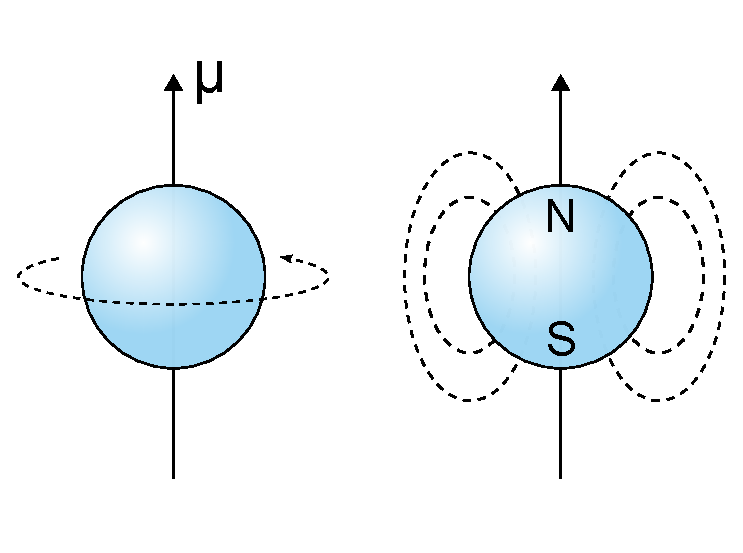
\includegraphics[width=3.5in]{mri/spin.pdf}
\end{tabular}
\caption{Spin of a nucleus has a magnetic moment vector $\mu$, which behaves similar to a magnet with north (N) and south (S) poles.}
\label{fig:spin}
\end{center}
\end{figure}

The spinning of nuclear particles produces angular momentum  $\textbf{J}$, that is a vector with both magnitude and direction. The largest measurable component of $J$, expressed as $I$, represents the overall quantized spin value as the spin quantum number. The corresponding quantum number is known as the magnetic quantum number $m$, and can take a total of $2I + 1$ angular momentum states.  A non-zero spin is associated with a non-zero magnetic moment ($\vec{\mu}$) via the relation $\vec{\mu} =\gamma \textbf{J}$. The z-component of the angular momentum vector (\textbf{J}) is $J_z = m \hbar$. The z-component of the magnetic moment $\mu_z$ is thus: 

$$\mu_z=\gamma J_z=\gamma m \hbar$$

Where $\gamma$ is the gyromagnetic ratio, $\hbar$ is the reduced Planck constant ($=1.0545726 \times 10^{-34} m^2kg/s$ ).

\subsubsection{Effect of Magnetic Field}

In the absence of an externally applied magnetic field, the magnetic dipoles are oriented randomly. When the proton is placed in an external magnetic field $B_0$, the spin vectors become oriented with the field, either parallel or anti-parallel with respect to $B_0$ (Figure \ref{fig:externalB0}). The nuclei precess about the magnetic field direction at some frequency called Larmor frequency: 

$$\omega = \gamma B$$.

Where $\gamma$ is the gyromagnetic ratio, and $B$ the magnetic field magnitude.


\begin{figure}[htb]
\begin{center}
\begin{tabular}{c}
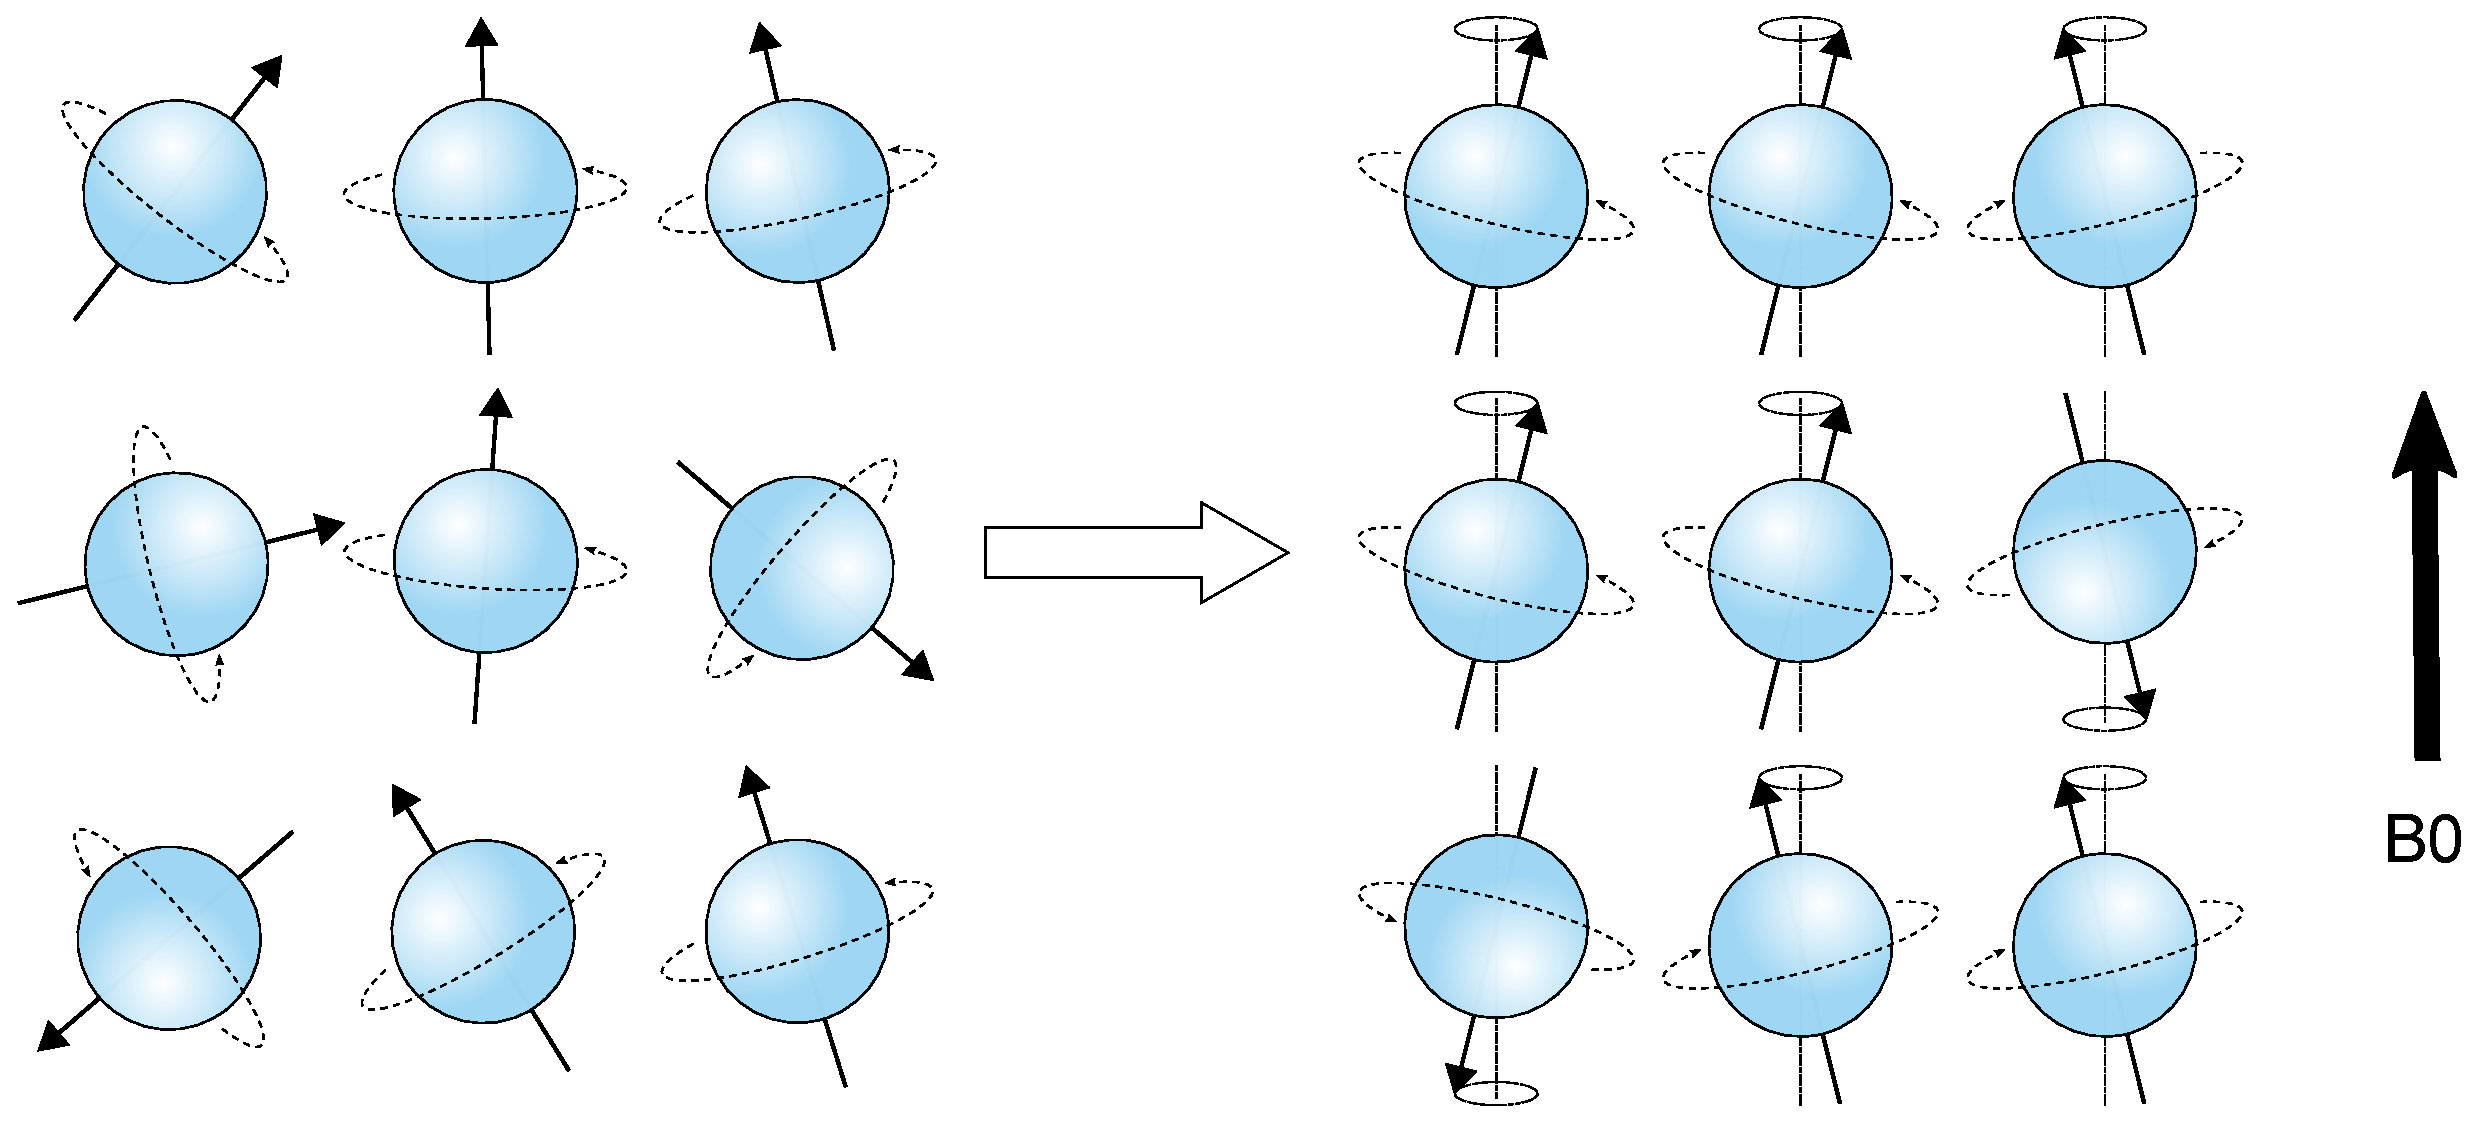
\includegraphics[width=4.5in]{mri/field.pdf}
\end{tabular}
\caption{Left panel-- magnetic moments with random orientations in the absence of external magnetic field; Right panel-- magnetic moments parallel or anti-parallel aligned with the external
field} \label{fig:externalB0}
\end{center}
\end{figure}

Protons aligned in the parallel alignment are more preferred as it has a lower energy state than in anti-parallel orientation. The energy E of a magnetic moment $\vec{\mu}$ when in a magnetic field $B_0$ is given by: $E=-\vec{\mu}\cdot \textbf{B}_0=-\mu_z B_0=-\gamma m \hbar B_0$. The lower energy state of protons corresponding to m = +1/2 in a static magnetic field $B_0$ is $E(\frac{1}{2})=-\frac{1}{2}\gamma \hbar B_0$. The higher energy state of protons corresponding to m =-1/2 is given by $E(-\frac{1}{2})=\frac{1}{2}\gamma \hbar B_0$.
Consequently, the energy differences between two quantum states can be calculated as $\bigtriangleup E = \gamma \hbar B_0$ (Figure \ref{fig:energy}).

\begin{figure}[htb]
\begin{center}
\begin{tabular}{c}
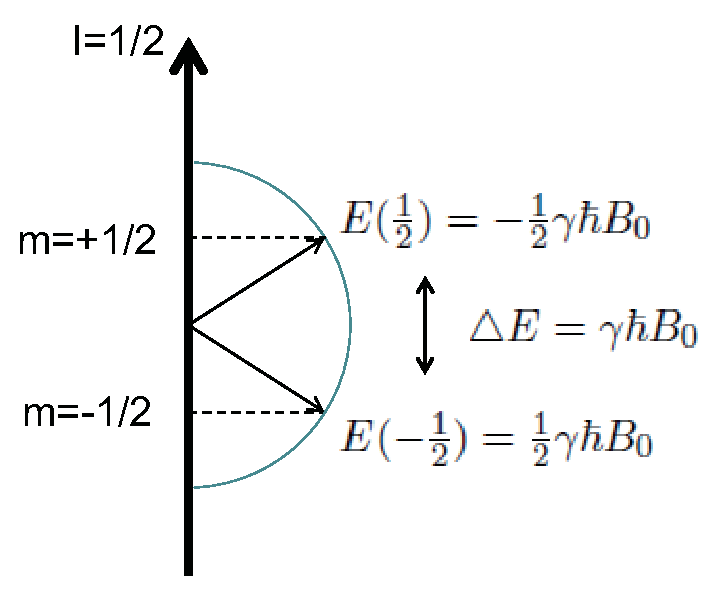
\includegraphics[width=3in]{mri/energy}
\end{tabular}
\caption{For protons with spin quantum number of 1/2, two energy
levels and the energy difference are shown.} \label{fig:energy}
\end{center}
\end{figure}

There are more protons with spins with parallel orientation than anti-parallel, due to the increased energy stability. This number of difference is called spin excess and the magnetic moments of the excess spins add to form the net magnetization vector $M_z$. When the spin system is at equilibrium, net magnetization lies along the z-axis, parallel to $B_0$.

\subsubsection{Resonance Condition}

The steady-state of the stable spin state under $B_0 $ can be disturbed by introducing additional energy $E$ into the system. 

The proton would undergo a transition from the lower energy to higher energy state by the absorption of a photon. The energy difference between the nuclear spin levels is $\bigtriangleup E = \gamma \hbar B_0$. Hence, a magnetic resonance absorption will only occur when $\nu_0 = \gamma B_0/(2 \pi)$, which is the same as Larmor frequency. This is called the \textit{resonance condition}. 

\subsubsection{Relaxation}
Transverse magnetization is introduced into the system that oscillates at radio frequency (RF) to modify the net magnetization, and this is called the RF pulse. When exposing the nuclear spin system to the energy of the RF pulse, the equilibrium of the spin system is disturbed. The RF pulse is designed to introduce energy E such that the net spin direction orients at $90^\circ$. The net magnetization now is denoted as $M_{xy}$ as it aligns with the xy-plane instead of the z-axis. Individual spins now precess in phase with the RF pulse, and it gives rises to the MR signal in the receiver coil. 

With the termination of the RF pulse, the nuclei in the excited state will return to the equilibrium condition. This process is called \textit{relaxation}. 
The energy transmitted decays rapidly by two relaxation processes:  spin-lattice and spin-spin relaxations. These are responsible for \textit{T1 relaxation} and \textit{T2 relaxation} respectively.

\paragraph{T1 Relaxation} 
As the transverse magnetization decays, the magnetic moment gradually realigns with the z-axis of $B_0$. 
The magnitude of the magnetic moment's xy-component also gradually diminishes, and the MR signal fades. 
The $M_z$ magnetic moment recovers in proportion, and is eventually restored. 
This processed is called \textit{longitudinal relaxation} or T1 recovery, where T1 refers to the mean time for an individual nucleus to
dissipate its excess energy (heat) to the surrounding environment ( the \textit{lattice}, and therefore the processed is also named \textit{spin-lattice relaxation})and return to its equilibrium state. 

\begin{figure}[htb]
\begin{center}
\begin{tabular}{c}
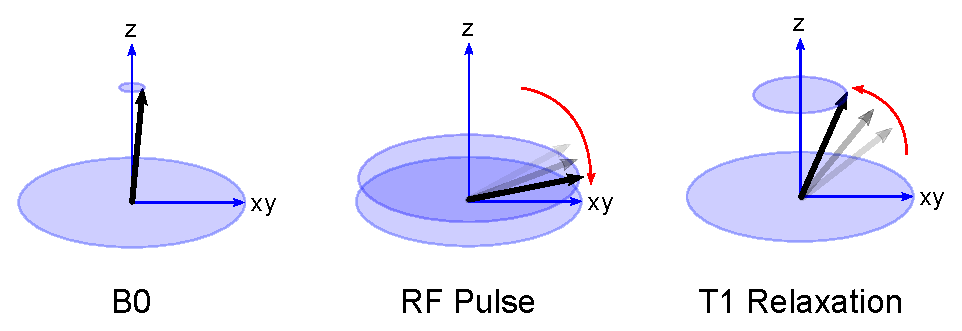
\includegraphics[width=\textwidth]{mri/rf-pulse.pdf}
\end{tabular}
\caption{Illustration of the process of transverse relaxation. Initially, the spin precesses about the B0 field under steady-state. When a 90deg RF pulse is applied, the spin orients towards the xy-plane. When the RF pulse is switched off, the spin now relaxes towards the z-axis.  } \label{fig:relaxation}
\end{center}
\end{figure}

To describe how $M_z$ returns from 0 to its equilibrium during relaxation, the equation as a
function with respect to time $t$ is written as: 
$$M_z = M_0 (1 - e^{-t/T1})$$
where T1 is the time taken for approximately 63$\%$ of the longitudinal magnetization to be restored (Figure \ref{fig:T1T2}(A)). 
$M_0$ is the magnetic moment at equilibrium. 

\paragraph{T2 Relaxation}

T2 relaxation is so named after the time constant of phase decoherence of the transverse magnetic moment. 

Immediate after excitation, the phase precessions are synchronous, and therefore are in \textit{phase coherence}.  
However due to various reasons, the various spins begin to lose coherence, and their total sum magnetization $M_xy$ diminishes. 

Phase coherence is lost in two ways:
\begin{enumerate}
\item Spins are associated with local magnetic fields, and interact randomly. The energy transfers that occur in the local magnetic field interactions cause a cumulative loss of phase. These are pure spin-spin interactions, and thereby not affected by $180^\circ$ refocusing pulse. They are also independent of the strength of $B_0$. 
The time constant which describes the return to equilibrium of the transverse magnetization is called the \textit{spin-spin
relaxation time} or T2, and is defined in respect to time $t$ as:
$$M_{xy} =M_{xymax} e^{-t/T2}$$
where T2 is the duration of time for the transverse magnetization to decay to 37$\%$ of its original magnitude. 
T2 is always less than or equal to T1.

\item There are intrinsic inhomogeneities by the magnetic field generator, and the scanning subject. These intrinsic properties contribute to the dephasing, and has a shorter time decay than T2. This type of decay time constant is named T2*  (Figure \ref{fig:T1T2}(C)). The loss of the MR signal due to T2* is called\textit{ free induction decay} (FID). T2* is defined as follows: 
$$ \frac{1}{T_2^*} = \frac{1}{T_2} + \frac{1}{T_2inhomo}$$ 
\end{enumerate}

\begin{figure}[ht]
\begin{center}
\begin{tabular}{c}
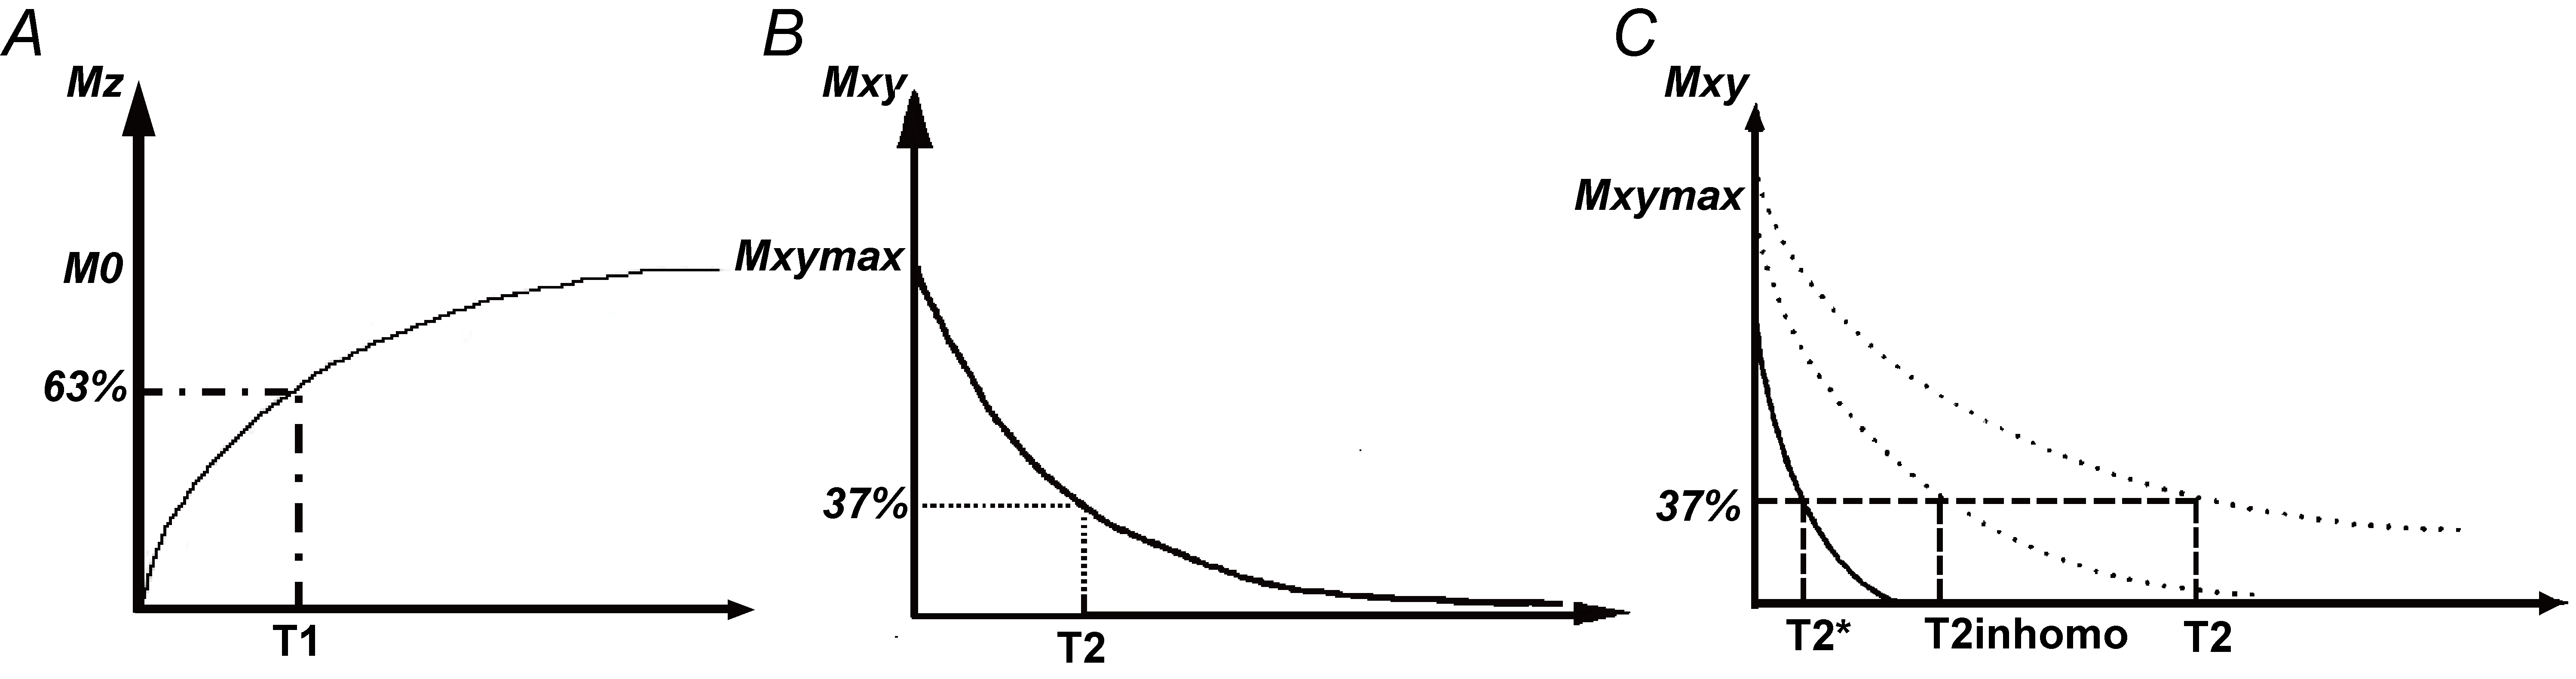
\includegraphics[width=5.5in]{mri/T1T2}
\end{tabular}
\caption{Diagram depicting the relaxation processes of T1 (panel A), T2 (panel B) and $T_2^*$ (panel C). $T_2^*$ is shorter than T2.} \label{fig:T1T2}
\end{center}
\end{figure}

\subsubsection{MR Contrast}

MRI signal intensity depends primarily on three parameters: 
\begin{itemize}
\item Proton density: the number of excitable spins per unit volume, which determines the maximum amount of signal that can be measured from the tissue. It can be measured by minimizing T1 and T2 times. 
\item T1 time: the amount time for $M_xy$ to recover to $M_z$, to be ready for re-excitation.
\item T2 time: the amount of time for $M_xy$ signal to fade under decoherence. 
\end{itemize}
The contrast in brain tissues of the resulting MR image can be tuned by adjusting these three parameters in pulse sequence design.

\paragraph{Repetition Time}
T1 contrast is adjusted by tuning repetition time (TR), which is the length of relaxation interval between excitation pulses. When TR is long (> 1500 ms), $M_z$ recovers totally, and therefore subsequent excitation will again retain maximal signal strength. When the TR is short (< 600 ms), the $M_z$ has not entirely recovered, and the next excitation pulse will not be able to regain signal strength. Different tissues have different intrinsic T1 differences, and will show strong contrast under short TR. Therefore short TR are said to be T1 weighted. 

\paragraph{Echo Time}
MR sequences have a gradient field which is used to control field inhomogeneities and to encode spatial origin. The gradients also contribute to spin dephasing. Therefore a refocusing pulse is necessary to measure MR signals adequately. The time delay between refocusing and the measured signal under phase coherence (spin echo) is known as echo time (TE). When TE is short ($<$ 30 ms), there are little signal differences between tissue types; when TE is long ( $\geq$ 60 ms ), the intrinsic tissue differences will allow good contrast in the resulting image. Therefore long TE is said to be T2 weighted.

\begin{figure}[htb]
\begin{center}
\begin{tabular}{c}
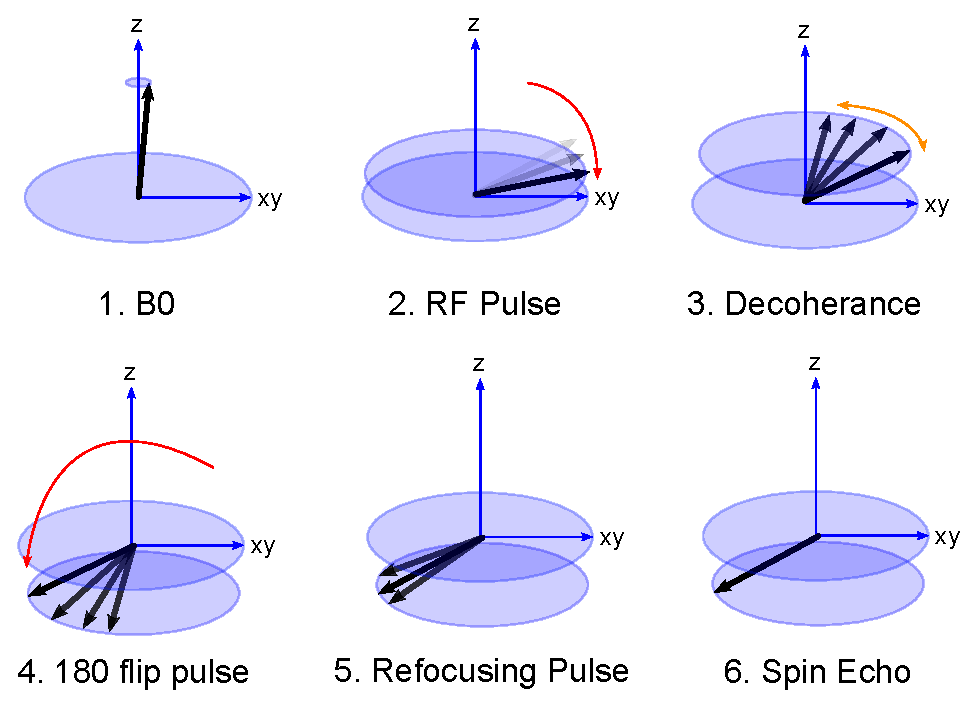
\includegraphics[width=\textwidth]{mri/spin-echo.pdf}
\end{tabular}
\caption{Illustration of the process of spin-echo. Initially, the spin precesses about the B0 field under steady-state. When a 90deg RF pulse is applied, the spins orients towards the xy-plane. When the RF pulse is switched off, the spins now relaxes towards the z-axis, and the spin undergoes phase decoherence. A 180 degrees flip angle pulse is applied to prevent spin saturation, and then a refocusing pulse is applied to bring spins back into coherence.  } \label{fig:spin-echo}
\end{center}
\end{figure}

Typically, T1-weighted spin echo (SE)  sequence is acquired with TR/TE at 340/13 ms; T2-weighted fast spin echo (FSE) at TR/TE of 3500/120 ms. 
In the case of T1-weighted MRI, images are created with short TE and short TR times. They can differentiate fat from water - with fat brighter and water darker (\url{www.mr-tip.com}) by using a gradient echo (GRE) sequence. In the brain T1-weighted scans provide good gray matter/white matter contrast. In addition, the image contrast can be increased with the use of an inversion pulse as in an MP-RAGE sequence. Due to short TR, this scan can be run very quickly, allowing the collection of high resolution 3D structural image (Figure \ref{fig:T1T2PD}, Left). These structural images can provide detailed information on the brain's shape and size, and provide the base for cortical surface reconstruction and segmentation. 

The T2-weighted sequence uses a long TR and long TE. The T2-weighted sequence can be employed as a dual echo sequence. Like the T1-weighted scan, fat is
differentiated from water, but with fat dark and water bright (Figure \ref{fig:T1T2PD}, Middle).  

The first or shorter echo ($T_E<30msec$) is proton density (PD) weighted or a mixture of T1 and T2. This image can provide good contrast of tissue and CSF, thus very helpful for evaluating periventricular pathology (Figure \ref{fig:T1T2PD}, Right). $T_2^*$-weighted scans use a gradient echo (GRE) sequence, with long TE and long TR. It is prone to susceptibility losses at air/tissue boundaries, but can increase contrast for certain types of tissue, such as venous blood. It is used for functional MRI detection allowing people to visualize and map the parts of the brain used to perform tasks. 

\subsubsection{3D encoding}

\paragraph{Slice Selection} Recall that the resonance condition can only be satisfied when the RF pulse is equal to the Larmor frequency of the nucleus precession under the magnetic field. 
Therefore, to allow slice discrimination, the magnetic field along the z-axis is made to be inhomogeneous by introducing a linear gradient field. It is an extra coil that adds or subtracts from the main magnetic field. With the linear gradient, only a particular portion of the z-axis would share a similar unique Larmor frequency, and can be selectively excited with an RF pulse. The steepness of the gradient determines the slice thickness, the steeper the gradient, the thinner the slices.  

\paragraph{Spatial Encoding}
Once the spins are excited and precess in the xy-plane, two additional gradients are applied to allow discrimination of signal measures per slice. 

\begin{itemize}
\item Phase encoding: The phase encoding gradient is applied in the y-direction. It alters the Larmor frequency of the spins based the location of the y-axis, and results in phase shifts of the spins relative to each other. The phase shift is determined by the duration and amplitude of the gradient, when the gradient is switched off, all spins return to their initial rate of precession, but maintains the relative phase shift. 
\item Frequency encoding: The frequency encoding gradient is applied on the x-direction. This applies a magnetic field that increases in strength from right to left. The change in Larmor frequency alters the precession speed of the spins such that the spins towards the right precess faster than that of the left. The MR signal collected represents the entire frequency spectrum of the spins. 
\end{itemize}

The measured MR signal with both encoding methods allows recovery of spatial information from the scanned area. Application of Fourier transform will decompose the signal into component frequencies along the frequency encoding direction (x). The phase distribution along each frequency provide information on the phase encoding direction (y). Decomposing the phase distribution requires another Fourier transform on the multiple scans of different phase gradient strengths. This is called two-dimensional Fourier transform (2D-FT), the number of phase gradient measures is called the phase encoding step. 

\paragraph{K-Space}

The collected MR data are encoded in a mathematical space termed the k-space. The k-space is a two-dimensional feature space, where the x-axis $k_x$ represent the measured frequency domain, and $k_y$ the phase domain. Each step in $k_y$ represents a single phase encoding step. The x-axis origin $k_x=0$ is the gradient iso-center, and the frequency distribution is symmetric about the x-origin. The 2D-FT operation is applied to the k-space to transform the frequency domain information into an image. 

\begin{figure}[htb]
\begin{center}
%\begin{tabular}{c}
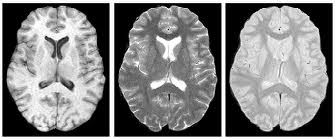
\includegraphics[width=5in]{mri/T1T2PD}
%\end{tabular}
\caption{Brain scan using T1 (left), T2 (middle) and proton density (right) measurements.}
\label{fig:T1T2PD}
\end{center}
%\vspace{-0.15in}

\end{figure}

\section{Diffusion Magnetic Resonance Imaging}

Diffusion magnetic resonance imaging (dMRI) is a popular MR modality that is capable of providing orientation information of brain white matter fibres \textit{in-vivo}, and thereby permitting the reconstruction and analysis of brain white matter structures with the use of computer reconstruction techniques. 

\subsection{Diffusion Weighted Image (DWI)}

DMRI is based on the observation that the location probability distribution of water molecules, which undergoes Brownian motion during diffusion, is a function of its suspension medium. The rate of diffusion can be formulated as \cite{Mukherjee2008}: 
\begin{equation}
<r^2>=6Dt
\end{equation}
where $<r^2>$ is the mean square displacement of the molecule after time $t$ with diffusion constant $D$. In an unhindered medium, such as in liquid water, the water molecule diffusion probability is can be described as an spherical volume, in other words it undergoes \textit{isotropic} diffusion. In biological tissue such as the neuron axonal bundle, water molecule diffusion probability is then constrained to be more likely in a direction along the bundle, rather than parallel to the cross-section, its diffusion state is then described as \textit{anisotropic} (\ref{fig:diffusion}). 

\begin{figure}[ht]
\begin{center}
\begin{tabular}{c}
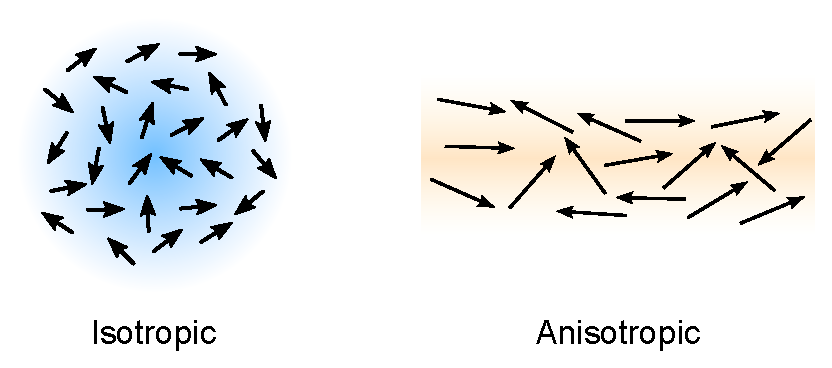
\includegraphics[width=0.8\textwidth]{diffusion.pdf}
\end{tabular}
\caption{Isotropic diffusion: diffusion of molecules have the same probable displacement in all directions. Anisotropic diffusion displacement of modules are constrained to its diffusion medium.}
\label{fig:diffusion}
\end{center}
\end{figure}

To image this difference in tissue diffusion, a diffusion-weighted imaging (DWI) pulse sequence, which is termed Stejskal-Tanner encoding, is used by adding diffusion-sensitizing gradients to a T2-weighted spin-echo sequence, before and after the 180 degrees refocusing pulse. The gradient is parameterized by the gradient amplitude $G$ in $mT/m$, duration $\delta$ in $ms$, and refocusing delay interval $\Delta$ in $ms$. 

The image contrast is determined by the amount molecular motion between the two diffusion gradients, where motion along the gradient axis results in a loss of signal intensity. The contrast is defined as: 
\begin{equation}
S_i = S_0 \cdot e^{-b \cdot ADC_i}
\end{equation}
Here $S_i$ denote the image contrast at a voxel. $S_0$ the signal intensity without the gradients applied. $ADC_i$ being the apparent diffusion coefficient in the $i$ direction. $b$ is the diffusion weighted factor that is a function of the duration, strength and temporal spacing of the gradients: 
\begin{equation}
b = \gamma^2 G^2 \delta^2(\Delta - \delta/3)
\end{equation}
where $\gamma$ is the gyromagnetic ratio constant. The ADC is measured in $mm^2/s$, and denotes the average molecular diffusion area with a given acquisition time. The higher ADC values indicate higher molecular mobility. Clinical DWI sequences typically use a diffusion time of 10-50 ms, or a travel of about 10$\mu$m. Typical clinical $b$ values range from 600 to 1500 $s/mm^2$, to balance signal contrast with acquisition time. 

\subsection{Diffusion Tensor Imaging}

To adequately characterize anisotropic diffusion, there must be more than one gradient directions available. In fact, it is possible to describe voxel-wise diffusion using a Gaussian diffusion model, where the diffusion anisotropy can be visualized as an ellipsoidal tensor \cite{Jones2002}. This type of imaging methodology is termed diffusion tensor imaging (DTI). At least six non-collinear gradient directions must be captured to compute the DT. In practice, up to 32 gradients directions are used clinically.

The diffusion tensor is a $3 \times 3$ symmetric matrix that describes diffusion displacement in the three major axes of diffusion: 

\begin{equation}
D=
\begin{bmatrix}
    D_{xx} & D_{xy} & D_{xz} \\
    D_{xy} & D_{yy} & D_{yz} \\
    D_{xz} & D_{yz} & D_{zz}
\end{bmatrix}
\end{equation}
Where $D_{i,j}$ is related to:

\begin{equation}
\frac{S}{S_0} = e^{-\Big(\sum\limits_{i=x,y,z} \sum\limits_{j=x,y,z} b_{i,j} \cdot D_{i,j}\Big)}
\end{equation}

and 

\begin{equation}
b_{i,j} = \gamma^2 G_i G_j \Big[ \delta^2 \Big( \Delta - \frac{\delta}{3} \Big) \Big]. 
\end{equation}

The diffusion tensor can then be diagonalized to find its eigen vectors, which are the principal axis of the diffusion ellipsoid, and from which we can obtain the eigen values (\ref{fig:tensor}): 

\begin{equation}
\Lambda = 
\begin{bmatrix}
\lambda_1 	& 0 		& 0 		\\
0 			& \lambda_2	& 0 		\\
0 			& 0 		& \lambda_3 \\
\end{bmatrix}
= R \cdot D \cdot R^T.
\end{equation}

The eigen values are measured in the same unit as ADC, which is in $mm^2/s$. Their corresponding eigen vector is denoted as $\hat{\lambda_i}$ They are ordered from the greatest to the least diffusivity magnitude. $\hat{\lambda_1}$ points to the orientation of the greatest diffusion direction, and therefore $\lambda_1$ is also referred to as "longitudinal" or "axial" diffusivity. $\hat{\lambda_2}$ and $\hat{\lambda_3}$ are the lesser orthogonal diffusion directions, and their mean magnitude gives rise to the cross-sectional, or "radial" diffusivity. 

\begin{figure}[ht]
\begin{center}
\begin{tabular}{c}
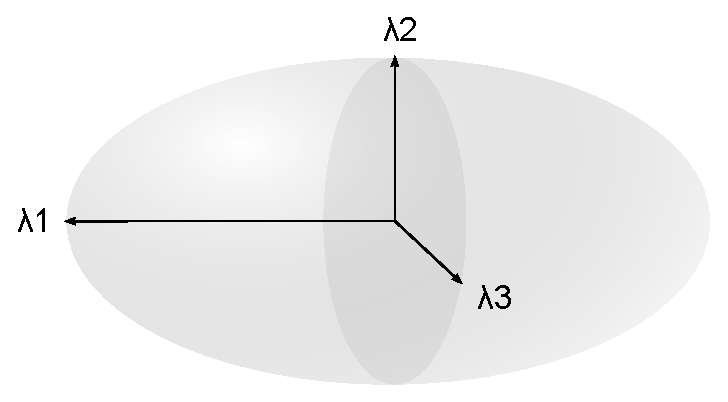
\includegraphics[width=2.5in]{tensor.pdf}
\end{tabular}
\caption{Illustration of the eigen vectors of an ellipsoid tensor.}
\label{fig:tensor}
\end{center}
\end{figure}

\subsubsection{DTI Metrics}

The Gaussian tensor eigen values form the basis of diffusivity measures that are commonly used to quantify cerebral tissue. The most common diffusivity metrics include Trace, Axial(Parallel/Primary/Longitudinal) diffusivity (AD), Radial (Perpendicular) diffusivity (RD), Mean diffusivity (MD) and fractional anisotropy, these are listed as follows: 

\begin{equation}
Trace = \sum_{i=1}^{3} \lambda_i
\end{equation}
\begin{equation}
AD = \lambda_1
\end{equation}
\begin{equation}
RD = \frac{(\lambda_2+\lambda_3)}{2}
\end{equation}
\begin{equation}
MD = \frac{\text{Trace}}{3}
\end{equation}
\begin{equation}
FA = \sqrt{\frac{3}{2}}\frac{\sqrt{(\lambda_1-MD)^2 + (\lambda_2-MD)^2 + (\lambda_3-MD)^2}}{\sqrt{\lambda_1^2+\lambda_2^2+\lambda_3^2}}
\end{equation}

Changes in white matter FA has been found to correlate with a wide spectrum of neuromorphological changes, including but not limited to multiple sclerosis \shortcite{Cercignani2001,Ciccarelli2003d,Miron2012}, vestibular schwannomas \shortcite{Chen2011b,Taoka2006,Wai2009}, tumors \shortcite{Mori2002,Schonberg2006,Nimsky2005}, schizophrenia \shortcite{Rametti2009,Fitzsimmons2009}, traumatic brain injury \shortcite{Bendlin2008,Kinnunen2011c,Hellyer2012}. RD is found to positively correlate with degree of demyelination in multiple sclerosis \shortcite{Song2005,Song2002,Klawiter2011,Janve2013}, and well as stages of white-matter development and aging \shortcite{Counsell2006,Sala2010}, including alzheimer's disease \shortcite{Acosta-Cabronero2012}. AD is correlated positively with axonal integrity \shortcite{Song2003}, and is found to be a correlate of axonal injury \shortcite{Budde2009} such as those found in traumatic brain injury \shortcite{Kinnunen2011c} and Gulf War illness \shortcite{Rayhan2013}. MD is correlated with tissue inflammation and edema \shortcite{Senda2012g}, and is found to correlate with diffusivity changes as a result of gliomas \shortcite{Stadlbauer2007}, multiple sclerosis \shortcite{Cercignani2001,Senda2012g,DeGroot2013}, amyotrophic lateral sclerosis \shortcite{Sharma2012}, and aging \shortcite{Kantarci2011}.

\subsubsection{Limitations}

DTI is based on the Gaussian model of water diffusion, and therefore imposes an important limitation. The Gaussian tensor can derive only one diffusion direction at a given voxel, and therefore is incapable of modelling cross-fibre diffusion of two or more directions. By extension, its derived metrics (FA, AD, RD) can only characterize a single diffusion direction as well. Therefore the interpretation of these metrics in white matter that contains cross-fibre configurations is tenuous.  

\subsection{High Angular Resolution Diffusion Imaging}

In order to characterize the additional diffusion components in voxels with multiple fibres, changes in DWI acquisition strategies is necessary. A natural extension is to acquire additional diffusion directions. This type of acquisition strategies, which enable higher order diffusion modelling algorithms, are generally referred to as high angular resolution diffusion imaging (HARDI). The most wide-spread strategy is to equally distribute gradient directions as vertices of a triangle-tessellated geodesic sphere \cite{Frank2001}. Alternatively, it is also possible to distribute gradient directions in a rectilinear grid, which forms the basis of diffusion spectrum imaging (DSI) \cite{Wedeen2005}. Additional acquisition strategies such as distributing gradient directions across multiple concentric spherical shells are also actively explored \cite{Jeurissen2014a}. 

Modifications to b-value needs to be considered for HARDI. The measured diffusion contrasts are dependent on the diffusion compartment variances. Therefore higher b-values will increase the measured signals variance contrasts, and allow better separation between crossing diffusion directions. Different HARDI algorithms have different requirements on b-values. For example Q-ball imaging needs b=3000 $s/mm^2$ \cite{Descoteaux2007a}, and multi-shell acquisitions will require stepped values of b-values ranging from 500  $s/mm^2 $  to greater than 3500  $s/mm^2 $ \cite{Tournier2013}. 

The determination of gradient sampling pattern and b-value directly affect acquisition time and image quality. More complex gradient sampling and higher b-values can improve tractography quality. However the acquisition time can become prohibitively long in a clinical setting. Other factors that must be considered include the nature of patient pathology, motion artifacts, and the inclusion of other imaging modalities during clinical scan sessions. 

\subsection{Spherical Deconvolution}

An end-to-end spherical deconvolution diffusion model was first proposed by Tournier et al. \cite{Tournier2004}. 
Consider a fibre population with distinct fibre components. The measured diffusion signal $S(\theta,\phi)$ can be written as:

\begin{equation}
S(\theta, \phi) = \sum_{i}^{} f_i \hat{A}_i R(\theta)
\end{equation}
where $\theta$ is the elevation angle,  $\phi$ the azimuth angle in spherical coordinates; $f_i$ is the volume fraction of the $i$-th fibre component, $\hat{A}$ is the rotation operator that orients fibre, and $R(\theta)$ is an axially symmetric response function. 

$S(\theta,\phi) $ can be rewritten as a convolution over the unit sphere of $R(\theta)$ with a fibre orientation density function (FOD) $F(\theta, \phi)$, such that:
\begin{equation}
S(\theta, \phi) = F(\theta, \phi) \otimes R(\theta)
\end{equation}

With this approach, the FOD can be estimated using the reverse spherical deconvolution, using spherical and rotational harmonics \cite{Healy1998}. Spherical harmonics are orthonormal basis functions over a sphere, and therefore can approximate any symmetric diffusion geometry in the spherical q-space. The rotational harmonics similarly form the orthonormal basis over all possible rotations, and can represent any symmetric fibre configurations. The harmonics have two important parameters: the harmonic order $l$ and phase factor $m$, with $ -l \leq m \leq l $ for each harmonic order level $l$. The odd $l$ harmonics represent antisymmetric functions, while the even $l$ harmonics represent symmetric functions (\ref{fig:harmonics}). 

\begin{figure}[ht]
\begin{center}
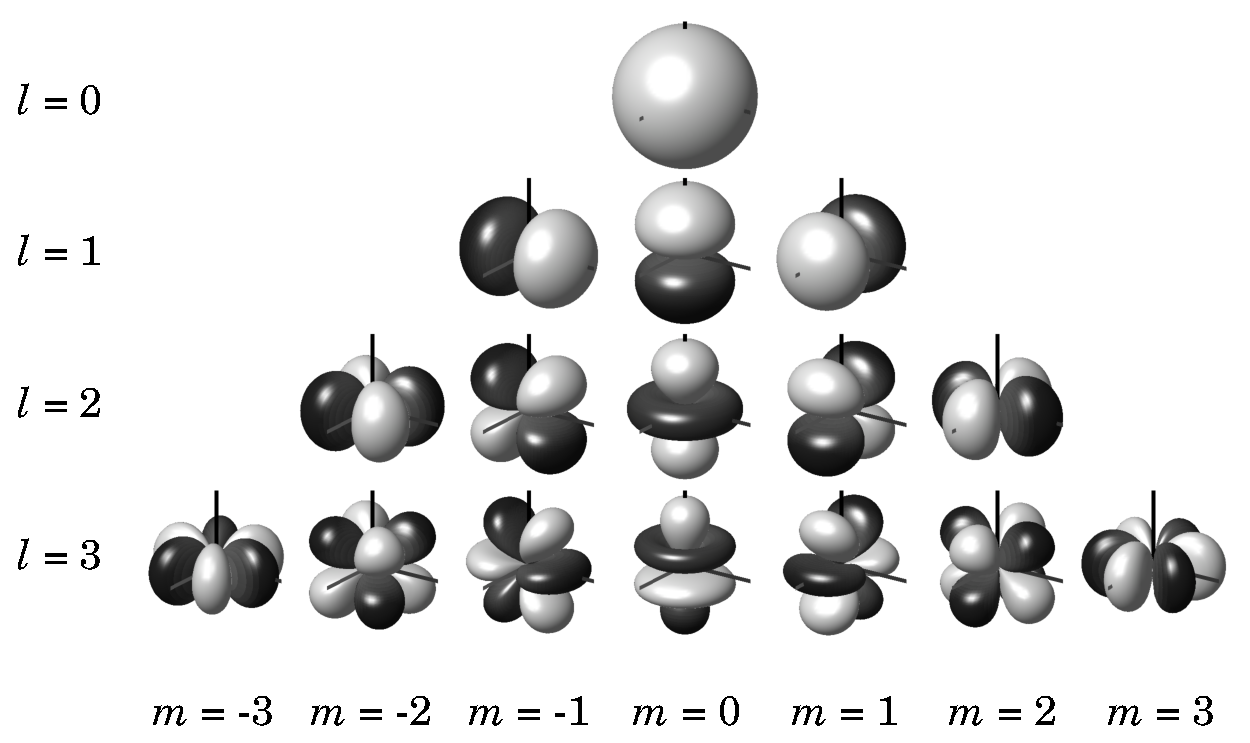
\includegraphics[width=\textwidth]{harmonics.pdf}
\caption{Visualization of the spherical harmonic functions up to l=3. Modified from \protect\cite{sh-image-wikipedia}}
\label{fig:harmonics}
\end{center}
\end{figure}

Spherical covolution is considered to be the action of a set of rotations on a function over a sphere. Given $F^l $ as a vector of $l$th order spherical harmonic decomposition of  $F(\theta,\phi)$, with vector length $(2l + 1)$, and $R^l$ as the $l$th order rotational harmonic decomposite of $R(\theta)$, with matrix size $(2l+1)^2$. The spherical harmonic representation of $S(\theta,\phi)$ is then:

\begin{equation}
S^l = R^l F^l
\end{equation}

To reduce the number of parameters to be computed, we can make the further assumption that the diffusion process is symmetric, and therefore the odd $l$ harmonic orders can be ignored, with only the even harmonics considered. 
The response function $R(\theta)$ can be directly estimated from the dataset by supplying DWI region with high anisotropy from a single fibre bundle, such as the body of the corpus callosum. 

The maximum harmonic order $l_max$ that can be estimated is dependent on the obtained number of directions. For example, $l_max$ = 8 requires 45 directions, $l_max$ = 10 requires 66 directions, and so on. Larger $l_max$ are more sensitive to noise, which is a weakness for the first spherical deconvolution algorithm \cite{Tournier2004}. 

\subsubsection{Constrained Spherical Deconvolution}
Further advances to the estimation method of the spherical deconvolution model made it more robust to noise \cite{Tournier2007b}. The noise of SD estimation is represented as spurious negative lobes in FOD, which are physically impossible, and do not represent any real phenomenon. To mitigate this, a non-negativity constraint is added. This method is referred to as \textit{constrained spherical deconvolution} (CSD). 

The CSD constraint is applied iteratively using Tikhonov regularization \cite{Hansen1998}. The procedure involves obtaining an initial FOD estimate, and a set of directional peaks are then identified. The Tikhonov regularization then constraints the negative peaks to zero, and a new set of FOD and peaks are obtained. The process is applied iteratively until convergence, and the final constrained FOD is obtained. 

The Tikhonov regularization minimizes the weighted sum with two terms:
\begin{equation}
\|{Af - b}\|^2 + \lambda^2 \| l(f - f')\|^2
\end{equation}
Where the first term is a linear least-square fit of solution $f$ to to data $b$ with problem matrix $A$. 
In terms of CSD, $f$ corresponds to the SH coefficients of the FOD, $b$ is the measured signal and $A$ is:
\begin{equation}
A = QR
\end{equation}
Where $Q$ is the SH coefficient to diffusion weighted intensity mapping, and $R$ is the spherical deconvolution. 
The regularization term is the constrained matrix $L$ multiplying the norm of $f$ relative to an initial estimate $f'$. The parameter $\lambda$ controls the regularization amount, with $\lambda=0$ having no regularization, to $\lambda\rightarrow \infty $ making the solution tend to $f'$. 

In CSD, the $f'=0$ and $L$ maps $f$ to orientations that have zero amplitude. During initiation, $f_0$ is estimated using spherical deconvolution with a low-pass filter \cite{Tournier2004}, and truncated to $l_max = 4$. The FOD amplitudes $u$ are then computed along N uniformly distributed directions (By default, MRTrix uses $N=300$) where
\begin{equation}
u = P f_i
\end{equation}
L is then formed as:
\begin{equation}
L_{m,n} = 
	\begin{cases}
		P_{m,n}, & u_m < \tau \\
		0 &	u_m \geq \tau 
	\end{cases}
\end{equation}
where $\tau$ is the amplitude threshold. In practice $\tau$ is set to 10\% of mean FOD amplitude. 
The improved iterative $f_i$ is then solved by incorporating the new FOD amplitude information by:
\begin{equation}
f_{i+1} = \text{argmin}\{ \|Af_i - b\|^2 + \lambda^2 \|L f_i\|^2  \}
\end{equation}
The FOD estimate becomes stable when matrix L converges, which take about 10 iterations. 

CSD is robust to noise at relatively low B-values, and is capable of good quality FOD estimates at $B=1000 s/mm^2$. This means that existing DTI protocols can be extended for high order HARDI tractography by simply increasing the number of directions. With CSD, a 60 direction DWI acquisition can be used to confidently derive FOD with $l_{max}=8 $, and up to $l_{max}=12$ with super resolution enabled \cite{Tournier2007b} (Figure \ref{fig:csd}). 

\begin{figure}[ht]
\begin{center}
\begin{tabular}{c}
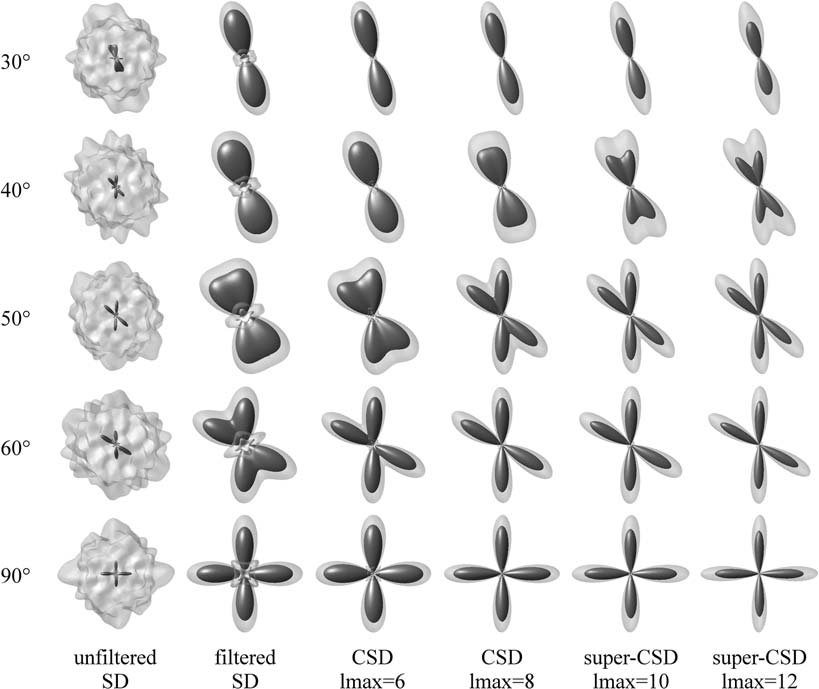
\includegraphics[width=\textwidth]{csd-angles}
\end{tabular}
\caption{ Comparison of angle discrimination ability and CSD FOD. B-value=3000 \protect $s/mm^2$. Taken from \protect \cite{Tournier2007b}. Reproduced with permission from Copyright Clearance Center (License ID: 4316770133531) } 
\label{fig:csd}
\end{center}
\end{figure}

\subsection{Tractography}

Tractography is a computer graphics technique used by neuroscientists to delineate neural pathways with DWI imaging. Applying pathway tracking to DWI imaging in the brain was first explored by Mori \cite{Mori2002b} and Basser\cite{Basser2000}. Tractography in essence is the construction, or propagation of streamline from an underlying field of orientation information, in order to visualize continuous structures within a volume.  The orientation field is generally provided as a 3D matrix of directional information obtained from DTI, CSD, or other methods. For example, in DTI the directions are the eigen vector with the greatest magnitude $\hat{\lambda_1}$; for CSD, the directional vectors would be peaks from the FOD. 

The family of methods that propagates by deterministic algorithms based on local orientation data is collectively called deterministic tractography. The first tracking algorithms were applied to DTI using step-wise polyline propagators that followed local DT tensors \cite{Conturo1999}. Further refinement of the line propagator to include neighbouring DT tensors, and interpolation of the local DT directions in order to obtain a smooth curve \cite{Mori2002b}. Basser introduced Runge-Kutta integration to allow more robust path-tracing when faced with noise in the local directions \cite{Basser2000}. Another similar path-integral method was also proposed by Tuch \cite{Tuch2000d}. The integrated tractography approaches are now standard practice for deterministic tractography \cite{Tournier2004,Pieper2004}. Deterministic tractography lends itself naturally to anatomical interpretation and further geometric analysis. It was traditionally paired with DTI, and so was thought to be limited in the case of crossing fibres. 

Other methods attempted to circumvent the limitation with probabilistic approaches that include white matter tissue priors in the fibre propagation model. The most popular of the probabilistic approach is the FSL software's probabilistic tractography module (FDT) \cite{Behrens2007}, which also includes a model-based ball-and-stick diffusion model that can resolve 2-fibre crossings. The FDT software produces visitation images of its probabilistic streams that collate the probability of tract propagation at each voxel. The visitation image, however, is hard to interpret and localize, and therefore does not rival deterministic methods in surgical visualization.

The availability of higher order HARDI methods, especially in CSD allows the reinterpretation of FOD as local fibre orientation probability distribution \cite{Tournier2010,Jeurissen2011b}. Development of a probabilistic streamline propagator based on CSD can now combine the advantage of probabilistic models with the geometric interpretability of deterministic tractography. 

\subsubsection{Applications}
Tractography permits the mapping of white matter pathway structures with computer graphic and statistic methods. It permits the study of brain structural connectivity at individual level \cite{Boorman2007} and group level \cite{Meskaldji2013},  circuitry mapping \cite{Kirsch2015} and macro-structural insights between the brain hemispheres \cite{Kucyi2012a}. It is often paired with functional connectivity for studies in multiple sclerosis \cite{Zhong2016,Rocca2007a}, chronic pain \cite{Mansour2013,Seifert2011,Wiech2014}, and other areas of study such as empathy \cite{Bernhardt2014}, and aphasia \cite{Catani2013c}.

Tractography is also capable of fine-grained neuroanatomy visualizations \cite{Hodaie2010, Chen2015c}, and therefore is important in the advancement of surgical visualization \cite{Chen2011b,Rosen2015,Hodaie2012g,Taoka2006,Sherbondy2008,Muthusamy2007} and planning \cite{Golby2011}. 

\begin{figure}[ht]
\begin{center}
\begin{tabular}{c}
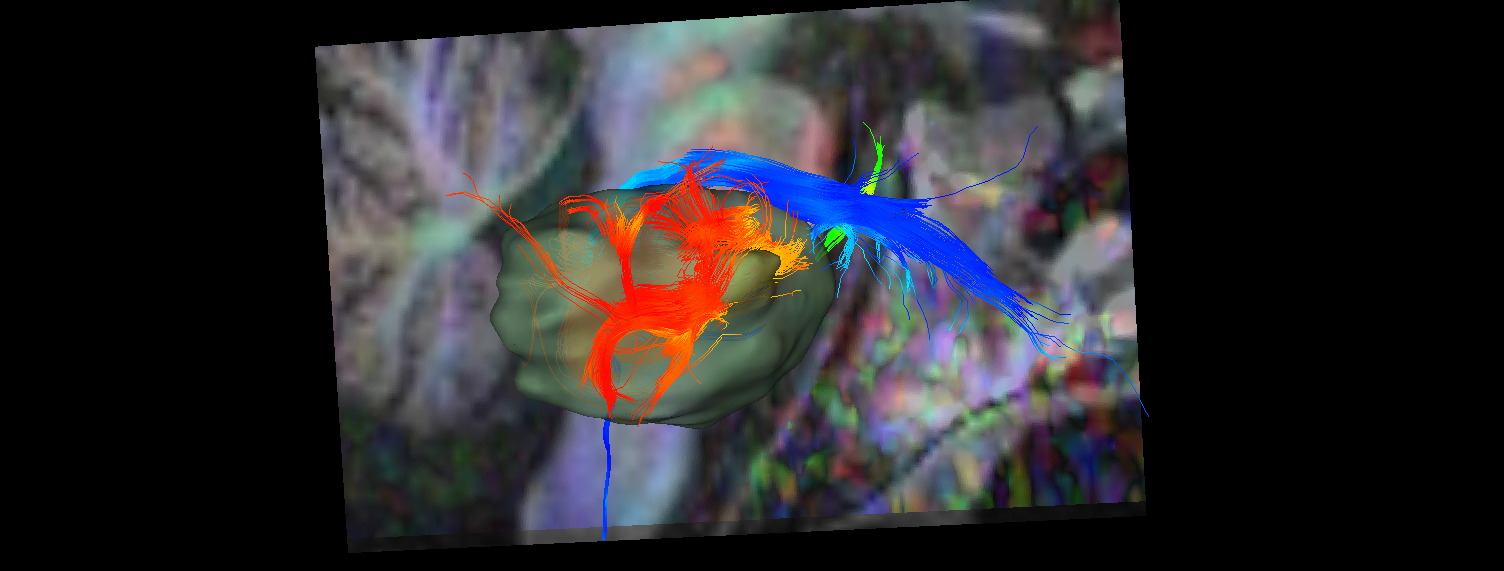
\includegraphics[width=\textwidth]{tractography1}
\end{tabular}
\caption{Example of cranial nerve reconstruction with deterministic tractography. The image represents a saggital view of a vestibular schwannoma (green) displacing the trigeminal nerve (blue) and the facial/vestibular nerve complex (red) at the level of the brainstem. } 
\label{fig:tract1}
\end{center}
\end{figure}


\section{Machine Learning}
Machine learning (ML) is a branch of computer science that aims to learn and form predictions from data. In contrast with static algorithmic programming, where the structures of the algorithms are predefined, machine learning approaches construct models based on observed data, in order to extend its predictions to the unobserved. Strategies and algorithms for constructing various models overlap with the fields of artificial intelligence, computational statistics, pattern recognition, and neuroscience. Advances in modern machine learning, especially in deep neural networks \cite{LeCun2015}, in recent years have led to wide-spread adoption of machine learning based online services in translation \cite{Bahdanau2014a}, image search \cite{simonyan2014very}, and speech recognition \cite{graves2013speech}. There is also surging interest in applying machine learning systems in medicine, particularly in radiology to assist in and disease diagnosis \cite{Kamnitsas2016,Suk2014}.

Machine learning training strategies can be categorized into Supervised Learning, Unsupervised Learning, and Reinforcement Learning. Supervised learning uses data that are pre-labelled according to some measure, in order to train a model. For example, the data supplied can be a list of patients' age and gender, and the label can be whether or not they are in pain. Unsupervised learning is a strategy that uses data without any prior labels, and the algorithm attempts to discover patterns embedded. Thus this approach is often used in data mining. Reinforcement learning involves continuously learning with a reward function. It is generally used to train autonomous agents using continuous streams of data, and is widely used in robotics.

\subsection{Supervised Learning}
Supervised learning is the most widely used method of training strategy. Most of the existing machine learning systems in production are based primarily on supervised training with human-supplied data labels. Different algorithms can be used to fit a function that forms a decision boundary based on data features and labels. Possible models range from Decision Trees, linear models such as Support Vector Machines (SVM), Deep Neural Networks (DNN), and bayesian-based models such as Naive Bayes and Gaussian Process (Figure \ref{fig:ml-bounds}).

\begin{figure}[h]
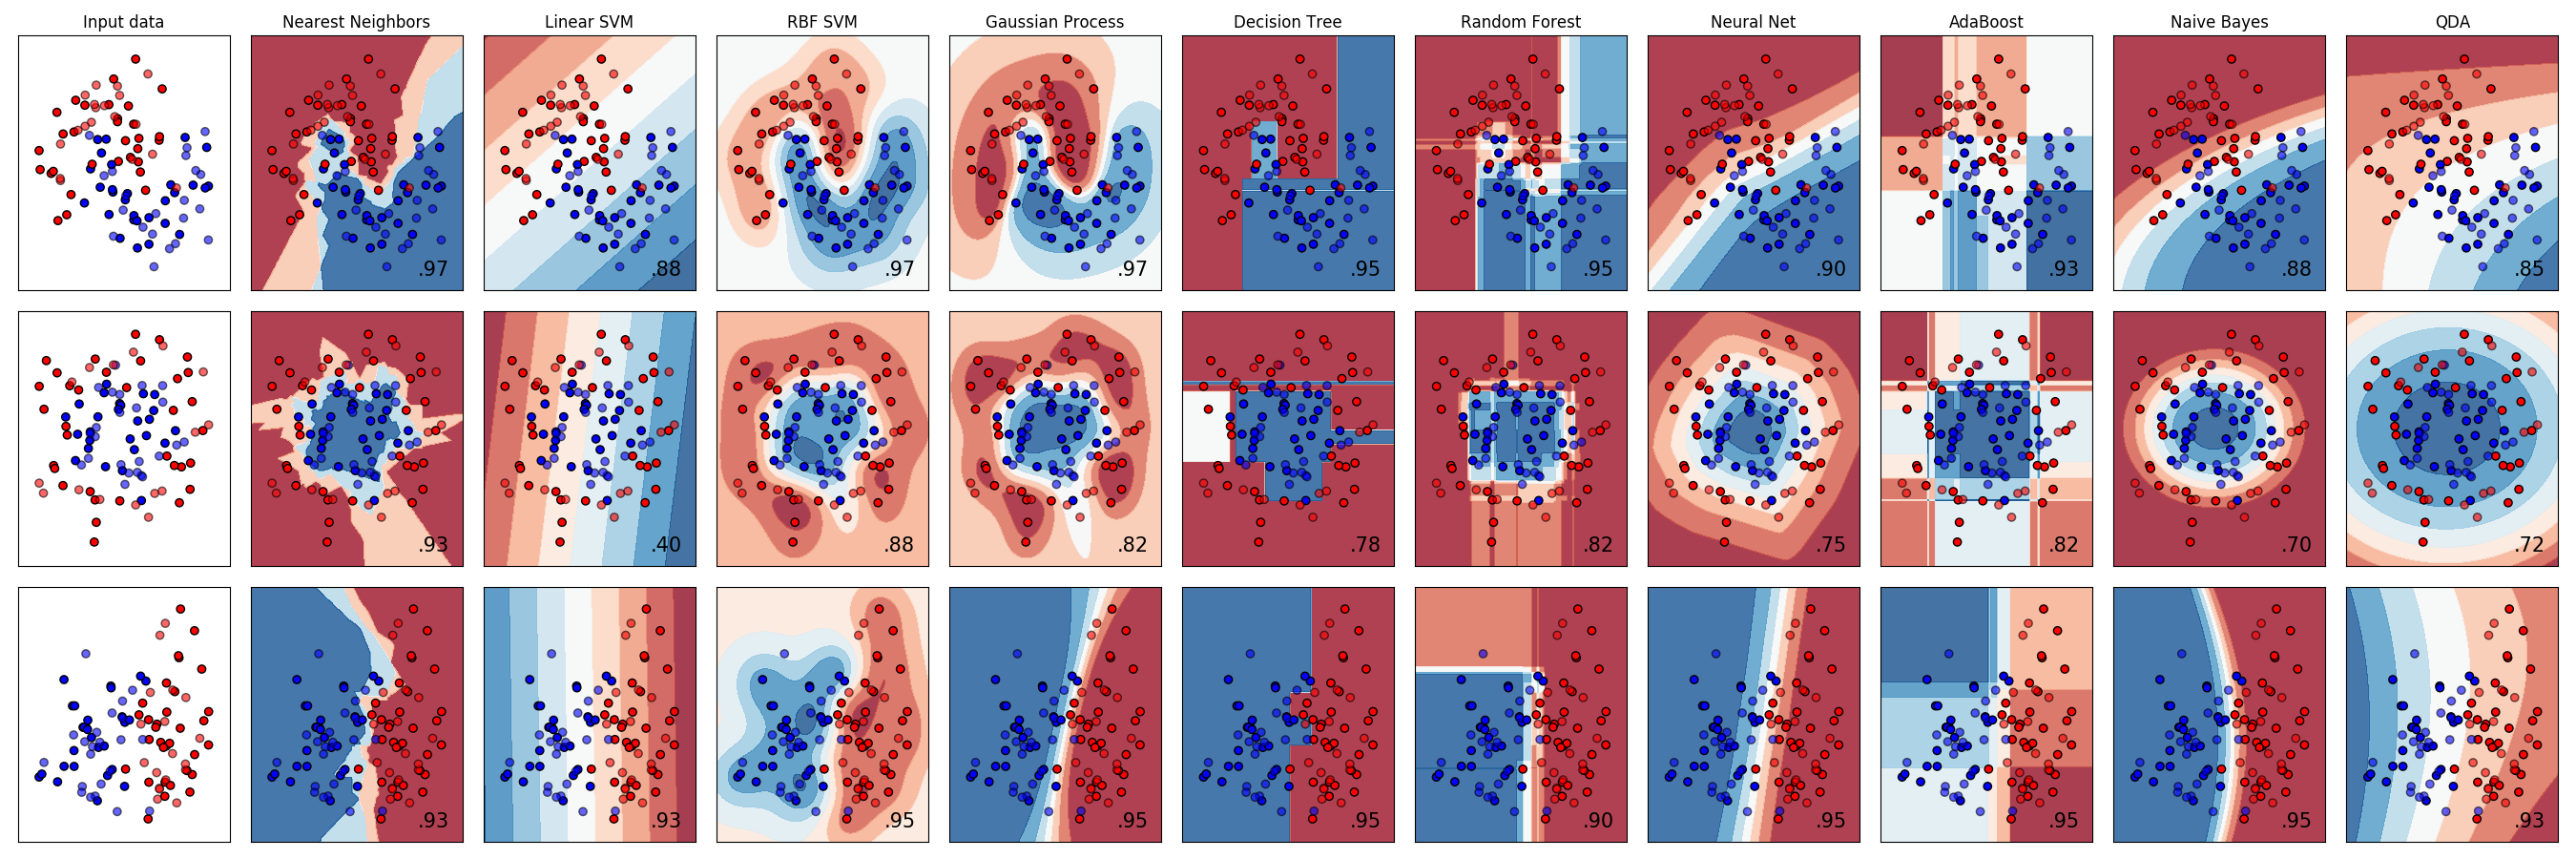
\includegraphics[width=\textwidth]{ml-decision-bounds.png}
\caption{Different of decision bounds as a result of different machine learning algorithms. Source: \protect\url{http://scikit-learn.org/stable/auto_examples/classification/plot_classifier_comparison.html} }\label{fig:ml-bounds}
 \end{figure}

\subsubsection{Gaussian Process}
The breakthrough results of deep convolutional neural networks in computer vision \cite{Krizhevsky2012} have sparked the interest of deploying similar systems for medical imaging diagnosis \cite{Greenspan2016}. However, one disadvantage of DNN is in its inability to quantify uncertainty and provide interpretable models. Model interpretability is a fundamental requirement for machine learning in medicine, and therefore there is renewed interest in bayesian-based models like Gaussian Process \cite{gal2016dropout}. DNN with an infinite number of hidden unit approximates GP \cite{neal1996priors}. 

Gaussian Process is defined as a collection of random variables, any finite number of which have a joint Gaussian distribution \cite{rasmussen2006gaussian}. 
It is a distribution that is defined by a mean function $m(x)$ and covariance function $k(x,x') $ where
\begin{equation}
	\begin{split}
		m(x) &= \mathbb{E}[f(x)], \\
		k(x,x') &= \mathbb{E}[(f(x)-m(x)(f(x')-m(x'))],
	\end{split}
\end{equation}
And the Gaussian Process is defined as
\begin{equation}
f(x) \sim GP(m(x), k(x, x')) 
\end{equation}

The covariance function is also termed called kernel function. The radial-basis function kernel or RBF kernel is widely used in machine learning tasks. The RBF kernel is also termed the square exponential, and is defined as

\begin{equation}
k(x, x') = exp\bigg( -\frac{1}{2}|x - x'|^2\bigg)
\end{equation} 

Another commonly used co-variance function is the Mat\'{e}rn kernel, which is used as an approximation for the RBF kernel in machine learning. It is defined, given a distance $r$ between two points, as:
\begin{equation}
k_{matern}(r) = \frac{2^{1-\nu}}{\Gamma(\nu)}\bigg(\frac{\sqrt{2\nu}r}{l}\bigg)^{\nu}K_{\nu}\bigg(\frac{\sqrt{2\nu}r}{l}\bigg)
\end{equation}
Where $K_\nu$ is a modified Bessel function \cite{rasmussen2006gaussian}. The Mat\'{e}rn kernel is equivalent to the RBF kernel when $\nu\rightarrow\infty$. In machine learning applications, $\nu$ commonly takes the value of $1.5$ or $2.5$ such that:
\begin{equation}
\begin{split}
k_{\nu=1.5}(d) &= \bigg(1+\frac{\sqrt{3}r}{l}\bigg)exp\bigg(-\frac{\sqrt{3}r}{l}\bigg), \\
k_{\nu=2.5}(d) &= \bigg(1+\frac{\sqrt{5}r}{l}+\frac{5r^2}{3l^2}\bigg)exp\bigg(-\frac{\sqrt{5}r}{l}\bigg), \\
\end{split}
\end{equation}
Where the function becomes once and twice differentiable respectively, and thereby having different degree of smoothness of approximation. 
 
\subsubsection{Training}
The process of fitting an ML model on labelled data to form predictions is called training. The objective of the training process is to obtain a model that can both correctly predict observed labels, and can generalize its predictions to new data that are not part of the training set. Depending on the model algorithm, there can be many training parameters that govern the model outcome. The tuning of these parameters is referred to as hyper-parameter tuning. It is possible for models trained with certain hyper-parameter combinations to result in model over-fitting, which is when a model is over-specialized in achieving the most accurate training label prediction, but perform poorly on unseen data. To properly evaluate model performance, a dataset is split into training/testing and validation sets, usually in 4:1 or 9:1 ratios, where model training is performed solely on the training set, and evaluation of model performance is on the validation set to assess the ability of the model to generalize.

There are instances when the number of available data is low, and each data point may have a substantial impact on model performance. In these cases, cross-validation is applied. The purpose is to divide the data into all possible combinations of training and validation splits, usually in the form of 5 fold to 10 fold. Then separate models are trained and evaluated on each combination, and their performance is averaged to form the final evaluation. This gives a reasonable approximate on the performance of the model when trained using all available data. Leave-one-out cross-validation is a special form where only one item is used for the validation split: given a dataset of N items, each split will consist of 1 and N-1 items, which result in N possible combinations. It is used when the available data are few. 
 
\subsection{Machine Learning, Neuroimaging, and Pain}

There is an extensive history of applying statistical methods to the field of neuroimaging, from the very onset of the field. Neuroimaging studies often attempt to correlate physiological and image-based measures with neuro-activities with specific experimental variables or conditions. Neuro-activities may be measured from EEG sensors, or as voxels in functional or structural MR images. Traditionally, data from each measured feature component was assumed to be independent. These components may be individual sensor readings or voxel-based measures. Correlative analysis were performed using general linear models, with post-hoc false-positive corrections. This type of univariate analysis does not have the ability to discover key relationships between feature components. Therefore univariate models cannot take into account spatial or temporally correlative dynamics. 

Increasing complexity in neuroimaging data has led to widespread applications of multi-variable machine learning methods in neuroimaging. Application of ML in pain neuroimaging became controversial when Tor Wager \cite{Wager2013} demonstrated a Lasso-PCA model that classified acute experimental pain with sensitivity and specificity of up to 90\% solely from fMRI imaging data. Additional studies showed consistently good performance of ML-based nociceptive pain discrimination. Detecting chronic pain proved to be more challenging, due to the high degree of similarity between acute and chronic pain fMRI activation patterns. The development of pain detection through brain imaging led to debates of the validity of presenting such methods as evidences in courtroom, where Davis et al argued against such actions \cite{Davis2012a,Davis2017}. While it is commonly accepted that pain evokes activity in the brain in multiple regions of the dynamic pain connectome, some studies suggest that the dorsal posterior-insula is heavily involved in chronic pain. Segerdale et al claimed that the dorsal posterior insula is a primary pain region \cite{Segerdahl2015a}, and this proposition ignited renewed debates surrounding regional specific brain centers for chronic pain \cite{Davis2015}.

Despite the controversies, interest in machine learning in medical imaging prognosis have sparked both public and private efforts across the globe. Classification studies using multi-modal data with features involving functional connectivity and structural connectivity in pain syndromes such as TN continue to improve. It is clear that machine learning is here to stay in pain neuroimaging research. 





\chapter{Aims/Hypotheses}

The general aim of this thesis is to introduce quantitative measures for the study of trigeminal nerve microstructure in health and disease. This necessitates detailed \textit{in-vivo} microstructural analysis of the nerve and its associated pathways, to determine how the microstructure is altered in idiopathic TN, symptomatic TN as a result of MS, and healthy controls. 

With an increasing number of subjects, single subject analysis becomes cumbersome. Critical methodological advances are necessary for the feasibility of the general aim. These include the development a group diffusion tractography tool, determination of the most robust intra-subject imaging co-registration strategy, and validation of the group tractography output across a variety of tractography algorithms and white matter anatomy. 

Lastly, these methodological advances will be applied to the large-scale study of TN versus healthy control.  The more considerable amount of data output from the methodology will enable the application of machine learning towards the aim of quantifying the specific group-wise diffusivity changes along the trigeminal sensory white matter pathways, in order to identify specific diffusivity pattern that differentiates between TN and non-TN. The roadmap and rationale for the specific studies are described below.

\section{Study I: Diffusivity signatures characterize trigeminal neuralgia associated with multiple sclerosis}
MS-TN is thought to relate to MS lesions in the brainstem, in the area of the trigeminal fibers in the pons. However the exact anatomical relationship between the lesions and trigeminal nerve within the brainstem has been difficult to quantify, due to the limited contrast and resolution in standard MRI and the variability of MS lesion across individuals. Previous single-tensor tractography studies of CN V have been limited to the imaging of the cisternal nerve segment. In this study, we use multi-tensor tractography with two aims: first, we focus on the delineation of the brainstem sub-segments of CN V; and the second, on the feasibility of applying multi-tensor tractography in the study of diffusivity differences in TN and MS-TN. 

\subsection{Main Aim} 
Establish the feasibility of multi-tensor diffusion tractography to delineating the cisternal, root entry zone and brainstem segments of CN V and how diffusivity changes in these sub-regions correlate with pain in MS-TN.

\subsection{Specific Aim}
\begin{itemize}
    \item Use multi-tensor tractography to delineate CN V into the the pontine brainstem, in order to quantify tissue diffusivity measurements in targeted sub-regions.
    \item Differentiate TN from MS-TN based on CN V diffusivity measurements.
\end{itemize}

\subsection{Specific Hypothesis}
\begin{itemize}
    \item TN is known to relate to vascular compression of the cistern REZ, therefore we expect its diffusivity signature to occur in the cisternal region.
    \item MS-TN should be related to brainstem MS lesions. Therefore CN V segments close to the lesions are expected to show more significant changes in tissue diffusivity, whereas segments far away from the lesions will not. 
    \item As a demyelinating disease, we expect to find a pattern of change in diffusivity signatures that reflects demyelination, including increase in RD, and decrease in FA. 
\end{itemize}

\section{Study II: Diffusion Weighted Image to T1 Co-registration Without Reversed-blip: Investigation of Best Practices}
The task of establishing inter-subject anatomical correspondences is imperative for extending tractography to multiple subjects. Population studies with inter-subject T1 registration are well-established, where a normalized T1 template is generated from numerous subjects to facilitate data analysis. Similarly, DWI of each subject can be co-registered to their corresponding T1, to extend the T1 template space to tractography space. Therefore the DWI-T1 co-registration accuracy is crucial to the reliability of inter-subject tractography alignment. DWI-T1 co-registration is challenging due to the DWI eddy-current and EPI field distortions. While new DWI sequences with reversed-blips have been shown to reduce non-linear distortions, they have yet to be commonly adopted in clinical practice. While T1 inter-subject registration methodology is well documented, the feasibility, and strategy for DWI-T1 co-registration on sequence without reversed-blips have not been documented, and forms a potential bottleneck on the performance of any DWI-T1 population registration pipeline.

\subsection{Main Aim}
Establish the best strategy to minimize DWI to T1 co-registration error in order to allow multi-modal template space registration across multiple subjects.

\subsection{Specific Aim}
\begin{itemize}
    \item Quantify the degree of improvement in registration between affine-only versus symmetric-diffeomorphic registrations.
    \item Determine which commonly-used DWI scalar image types can provide the best registration result when used as the registration-intermediate.
    \item Determine if anisotropic-power image, an experimental DWI scalar map that closely resemble T1 contrast, can provide even more registration improvements. 
\end{itemize}

\subsection{Specific Hypothesis}
\begin{itemize}
    \item Symmetric-diffeomorphic registration will result in the best accuracy, but with limited asymptotic improvement over affine registration alone.
    \item Averaged DWI should be the best scalar image, as it provides a balanced contrast between white and grey matter.
    \item Anisotropic-power (AP) image will show more substantial improvement over the existing scalar images.
\end{itemize}

\section{Study III: Merged Group Tractography Evaluation with Selective Automated Group Integrated Tractography}
The construction of an automated group tractography software framework depends on CN V brainstem delineation using multi-tensor tractography and the optimal DWI-T1 co-registration strategy. The aim is to create and validate a software framework that automates the tractography process on a large-scale, and also streamline research workflow by providing region-of-interest, and tractography parameter management. The software also provides the ability to report the tractography output at a group level both visually, as well as quantifying the consistency of group tractography output by developing a rating score called Normalized Overlap Score (NOS) score. 

\subsection{Main Aim}
The aim of this study is to validate and demonstrate the software's flexibility by comparing the performance of four tractography algorithms across six anatomical regions in a healthy population. The validations are performed  at a scale that would be prohibitive with manual methods. The comparisons determine the best tractography methods to use for different types of neuroanatomy.

\subsection{Specific Aim}
\begin{itemize}
    \item Compare DTI, XST, deterministic constrained-spherical deconvolution (CSD), and probabilistic CSD. 
    \item Use the above techniques to delineate a series of white matter tracts that have been challenging to delineate in full detail, including: fornix, facial/vestibular-cochlear cranial nerve complex, vagus nerve, rubral-cerebellar decussation, optic radiation, and auditory radiation.
    \item Validate normalized overlapping scores (NOS) by comparing merged tractography derived NOS scores with manual rating by neuroanatomy experts.
\end{itemize}

\subsection{Specific Hypothesis}
\begin{itemize}
    \item DTI is known to not able to delineate cross-fibers regions. If the group tractography works consistently, then its output should reflect such known algorithmic limitations, and DTI group tracts should not be able to perform well on more complex anatomies. The grouped tracts should however show consistent regional anatomical overlap across individuals.
    \item By merging the tracts of many individuals, the tractography delineations can complement each other, and this may improve the anatomical fidelity over individual cases.
    \item Specific tractography algorithms may be preferentially suited for the visualization of specific areas in the brain. For examples, deterministic tractography should preferentially be more suitable for nerve tractography, and probabilistic method better for deep neural pathways such as the optic and auditory radiations.
    \item NOS score should correlate with expert ratings, and show improved rating consistency over human rater variability.
\end{itemize}

\section{Study IV: Gaussian Process Classification of Trigeminal Neuralgia With Merged Tractography}
The developed methodology is applied to the study of the trigeminal sensory pathway. The method used is now thoroughly tested, and the best-suited tractography methods determined from the previous study. This study aims to examine the diffusivity signature differences in the trigeminal sensory pathway between TN and controls in a larger group. The pathway is divided into three major regions: CN V, trigeminopontothalamic (TPT) segment, and the thalamocortical S1 segment. Along-the-tract analysis are carried out by dividing each segment into 30 subdivisions. Following this, we use machine learning algorithms to auto-determine relevant subdivisions that maximally differentiates TN from controls.

\subsection{Main Aim}
The aim of this project is to reconstruct the trigeminal pathways from the cisternal segment to the level of S1 sensory cortex, and to examination these pathways using Gaussian Process classification to determine the subdivisions along each pathways that maximally differentiates TN from controls.


\subsection{Specific Aim}
\begin{itemize}
    \item Delineate and visualize the three segments of the trigeminal sensory pathway: CN V, trigeminopontothalamic and  thalamocortical S1 segment. 
    \item At each segment, identify microstructural features to distinguish the affected vs. unaffected sides.
\end{itemize}

\subsection{Specific Hypothesis}
\begin{itemize}
    \item To validate the study, CN V diffusivity signature should match findings from Study I.
    \item At the level of CN V, the affected cistern segment should show differentiation from the unaffected side.
    \item The affected S1 segment should differ from the unaffected side.
    \item The affected TPT segment might show more differentiation near the end points, due to possible differences in trigeminal nucleus and thalamus diffusivity. However, its mid-segment diffusivity might be inconclusive, as the diffusivity metrics such as FA and RD might not be adequate in describing the complex crossings at the pontine decussation. 
\end{itemize}

\graphicspath{{thesis/images/mspaper/drafts/}}

\chapter{STUDY I: Diffusivity signatures characterize trigeminal neuralgia associated with multiple sclerosis}
\chaptermark{Study I}
\label{section:study1}

This study was published in Multiple Sclerosis Journal \textcopyright 2016:

\bibentry{Chen2016a}


\section{Abstract}
\textbf{Background: }Trigeminal neuralgia secondary to multiple sclerosis (MS-TN) is a facial neuropathic pain syndrome similar to classic trigeminal neuralgia (TN). While TN is caused by neurovascular compression of the $5\textsuperscript{th}$ cranial nerve (CN V), how MS-related demyelination correlates with pain in MS-TN is not understood. 

\textbf{Objectives: }We aim to examine diffusivities along CN V in MS-TN, TN and controls in order to reveal differential neuroimaging correlates across groups.

\textbf{Methods: }3T MR diffusion weighted, T$_{1}$, T$_{2}$ and FLAIR sequences were acquired for MS-TN, TN, and controls. Multi-tensor tractography was used to delineate CN V across cisternal, root entry zone (REZ), pontine, and peri-lesional segments. Diffusion metrics including FA, RD, AD and MD were measured from each segment. 

\textbf{Results:} CN V segments showed distinctive diffusivity patterns. The TN group showed higher FA in the cisternal segment ipsilateral to the side of pain, and lower FA in the ipsilateral REZ segment. The MS-TN group showed lower FA in the ipsilateral peri-lesional segments,  suggesting differential microstructural changes along CN V in these conditions. 

\textbf{Conclusions:} The study demonstrates objective differences in CN V microstrucuture in TN and MS-TN using non-invasive neuroimaging. This represents significant improvement in the methods currently available to study pain in MS. 

\section{Introduction}
Trigeminal neuralgia is a neuropathic pain disorder characterized by severe, lancinating, facial pain with no major clinical sensory deficits. The pain occurs in one or more territories of the branches of the 5th cranial nerve (CN V) and is often triggered by innocuous stimuli, such as a light touch to the face. Classic trigeminal neuralgia is presumed to occur as a result of neurovascular compression at the root entry zone (REZ) of CN V (also referred as ‘idiopathic’; henceforth referred to simply as TN)(M Hodaie \& Coello, 2013). TN pain symptoms can also occur secondary to multiple sclerosis (MS-TN), where MS patients have a 20-fold risk of developing TN pain than the general population (up to 0.1\%)\cite{VanHecke2014}. 
While experientially similar, the pathophysiology of MS-TN differs from TN and involves CNS demyelination\cite{lazar1979trigeminal,Nurmikko2009}. The manner in which CNS demyelination results in pain is unclear. Brainstem plaques can be common in MS, but not all MS patient with brainstem plaques suffer from MS-TN. Furthermore, the presence of bilateral plaques does not clearly correlate with bilateral MS-TN pain\cite{DeSanti2011a,Love2001a}, highlighting the complex and uncertain relationship between the presence of plaques and pain\cite{DaSilva2005}. Importantly, this also highlights the fact that conventional MR plaque visualization does not fully correlate with MS clinical symptoms or their severity, and so improved neuroimaging methods are needed\cite{Seixas2014}. As classic TN is most commonly associated with vascular compression at the trigeminal nerve root entry zone, it is possible that in some MS patients neurovascular compression can also be present, adding further complexity to the diagnosis and treatment of trigeminal pain\cite{Sandell2010e}.

Understanding the microstructural anatomy of the trigeminal fibres is essential to determine how MS affects CN V brainstem fibres and how alterations to CN V in MS are related to the clinical presentation of pain. Direct comparisons between TN and MS-TN at the level of CN V brainstem fibres has been challenging because it is difficult to reliably identify, segment, and measure trigeminal anatomy with conventional magnetic resonance imaging (MRI)(Figure 1A-B)\cite{Cruccu2009,DaSilva2005}. Conventional MR imaging cannot visualize in isolation the brainstem fibres of CN V. Furthermore conventional tractography cannot resolve the brainstem crossing fibres\cite{Farquharson2013}, which leads to unreliable CN V delineations within the brainstem, and inaccuracies in diffusivity measurements. 

Diffusion tensor imaging (DTI) metrics, based on estimating the Gaussian diffusion of water in the neural tissue, can provide important insights to microstructural neural tissue changes in both pathological and normal states. Metrics including fractional anisotropy (FA), and radial (RD), axial (AD), and mean diffusivities (MD), reflect diffusivity change measured as a parameter of the estimated Gaussian diffusion tensor eigenvectors.  FA reflects the shape of the ellipsoid Gaussian tensor as a measure of anisotropy, and is correlated with both structural and cognitive changes that follow adverse brain changes such as traumatic brain injury, aging and Alzheimer’s disease\cite{Bendlin2008,Charlton2006,Kinnunen2011c,Mielke2012}. RD is a measure of the cross-sectional diffusion as an average of the second and third diffusion eigenvalues, and has been shown to positively correlate with axonal demyelination \cite{Song2002,Song2005}. AD is the greatest diffusion eigenvalue and has been positively correlated with axonal degeneration\cite{Budde2009,Song2002}, and MD is the mean of all three diffusion eigenvalues and is related to the increase in tissue inflammation and edema\cite{Beaulieu2002}. In MS studies, FA, RD and MD appear abnormal in or near MS lesions. The changes in diffusivity alter the Gaussian tensor profile and results in decreased FA, increased RD and increased MD\cite{Braley2012,Janve2013,Klawiter2011,Lin2007,Senda2012g}. While AD is generally not correlated with demyelination\cite{Song2002}, there have been findings associating decreases in AD with the presence of neurological damage in MS\cite{Budde2008,Kim2006}. 

The major technical limitation of diffusion tractography to date has been the inability of resolving crossing fibres using a single tensor Gaussian diffusion model\cite{Farquharson2013}, which has proved unsuitable for the visualization of brainstem tracts. However, techniques that use high angular resolution imaging  with an increased number of gradient directions acquired during diffusion weighted imaging (DWI), and advances in multi-tensor tractography (MTT) have improved the ability to delineate fibres in brain regions that have dense fibre crossings, such as the brainstem \cite{DellAcqua2007,Descoteaux2009c,Fillard2011,Qazi2009}. The microstructure of CN V in TN has recently been shown to be abnormal in terms of DTI metrics in the trigeminal REZ\cite{Desouza2013}. DTI metrics, as correlates of microstructural anatomy, are also important in identifying the nerve in pain in TN\cite{Hodaie2009a}. 

In this study of MS-TN, we hypothesize that A) myelination correlates of the trigeminal brainstem fibres, assessed with diffusion metrics, will reveal a pattern which is unique to MS-TN, despite inherent differences in precise lesion location, and B) diffusion metrics along the nerve will help differentiate between TN, MS-TN and healthy subjects, and may in future serve as a neuroimaging signature of pain in these populations. 
We used MTT and diffusivity metrics to identify specific neuroanatomical diffusivity differences between TN and MS-TN. Specifically, our aims were: 1) Visualize the isolated tracts of brainstem trigeminal fibres using MTT; 2) Sample and compare CN V diffusivities in MS-TN between symptomatic (+) and asymptomatic (-) sides of a) CN V at the REZ, b) brainstem CN V segments unaffected by MS plaques, and c) brainstem CN V segments with the presence of MS plaques; 3) Contrast diffusivity findings with CN V diffusivities in TN patients, MS-TN patients and healthy controls.

\section{Methods}

Magnetic resonance images were acquired using GE Signa HDx 3T scanner with an 8 channel head-coil. MR sequences were acquired from 3 groups (n=10 in each): unilateral MS-TN (4 males, 6 females; mean age  $53\pm8.6$ years) with no evidence of neurovascular compression of CN V at the REZ, unilateral TN (3 males, 7 females; mean age $57.1\pm8.5$ years), and healthy controls (3 males, 7 females; mean age $55.8\pm7.4$ years). Clinical pre-screening of MS patients and their associated lesion locations were performed using T$_{2}$ and FLAIR sequences. However clinical T$_{2}$ slice thickness was too large (\textgreater 3 mm) for proper assessment of 3D lesion volume. Therefore once the lesion was identified, the fast spoiled gradient echo (FSPGR) T$_{1}$ anatomical image was registered to the diffusion image in order to localize the MS lesion across multiple modalities for ROI placement. DWIs were acquired with 1 B$_{0}$ scan, 60 gradient directions, 3mm slice thickness and in-plane resolution of 0.9375$\times$0.9375 mm, b$_{0}$=1000 s/mm$\textsuperscript{2}$, TE=88.6 ms, TR=17000 ms, flip angle=90 deg, matrix=128$\times$128. T$_{1}$ FSPGR anatomical scans were acquired with 1mm slice thickness and in-plane resolution of 0.9375$\times$0.9375mm, slice spacing=1 mm, TE=5.052 ms, TR=11.956 ms, flip angle=20 deg, field of view (FOV)=240 deg, matrix=256$\times$256. T$_{2}$images were acquired with 4mm slice thickness, in-plane resolution=0.4297$\times$0.4297 mm, TE=94.14 ms, TR=5200 ms, flip angle=90 deg, FOV=170 deg, matrix=512$\times$512. FLAIR images were acquired with 4mm slice thickness, in-plane resolution=0.4297$\times$0.4297 mm, TE=141.4 ms, TR=8652 ms, flip angle=90 deg, FOV=220 deg, matrix=384$\times$224.

Images were analyzed with 3D Slicer (NA-MIC©, http://www.slicer.org)\cite{Pieper2004}. DWI sequences were corrected for eddy-current and motion distortions with appropriate corrections to gradient vectors, and imported into 3D Slicer for single-tensor diffusion tractography (SDT), where tracts were generated with initial seed spacing=0.5 mm, initial seeding FA threshold=0.2, stopping FA threshold=0.1, curvature threshold=0.8 and integration distance=0.1. Region-of-interests (ROI) seeding points were generated at a spacing of 0.25mm, or 64 points per voxel; MTT propagations were initiated at C1 threshold=0.2, tensor fraction=0.2, curve radius=0.8 rad, minimal length=10 mm, step size=1 mm. T$_{1}$ anatomical images were registered to the DWI using rigid transformation. To generate CN V tractography, ROIs were placed bilateral at the CN V at the REZ, and were used for both SDT and MTT. 

Diffusion parameters (FA, AD, RD, MD) were measured from 4 sets of pre-defined bilateral ROIs (Figure~\ref{fig:MSfigure1}C-D). Cross-sectional areas were based on tractography delineations, and thickness of 2 voxels. Location of the ROIs were defined based on trigeminal anatomy: 1) The cisternal ROI is measured from the nerve segment situated within the cisternal space surrounding the pons, at the mid-point between the Gasserian ganglion and the root entry zone; 2) the REZ ROI is defined at the junction where the CN V crosses from the cisternal space into pontine brainstem. This is where the neural myelination transitions from peripheral myelination (Schwann cells) to central myelination (oligodendrocytes). The ROI must include the cisternal segment and pontine segment at the transitional zone; 3) the pontine ROI is defined in the intra-pontine CN V segment at the mid-point between the REZ and the trigeminal nucleus. In MS-TN patients it is defined as the mid-point between the peri-lesional ROI and the REZ along the nerve that is not visually affected by any MS lesions (and note that subjects with MS lesions that did not allow ROI placement with at least 2 voxel spacing from peri-lesional and REZ ROIs were excluded as confounders); and 4) the peri-lesional ROI is defined as the intra-brainstem CN V segment at the closest proximity to MS lesions in its vicinity. In TN and control subjects, the corresponding ROI was the nerve segment closest in proximity to the trigeminal nucleus. In these patient groups, the pontine and peri-lesional areas are referred to as distal and proximal brainstem ROIs, respectively. 

Statistical analysis were performed using R statistics software suite(R Development Core Team, 2012). Segments and diffusivity measurements were analyzed separately. Patient group is considered an independent and between-subject factor; symptomatic and asymptomatic sides within the same patient are considered within-subject measures; in controls, the mean measures of left/right sides are used for comparison against other groups. A linear mixed model\cite{Pinheiro2011} is used to determine the statistical significance of within- and between-subject effects. Post hoc analyses were performed using pair-wise Student’s t-test, where multiple comparisons are corrected with false discovery rate correction\cite{Hothorn2008}. Statistical results were plotted\cite{Hunter2007} as diffusivity difference estimate matrices between anatomical regions and different subject groups. Values are mapped as red/blue based on mixed linear regression estimates. Positive estimates, where the group diffusivity parameter is greater in the vertical axis versus the horizontal axis are in red, and negative coefficients are in blue. 


\begin{figure}[p]
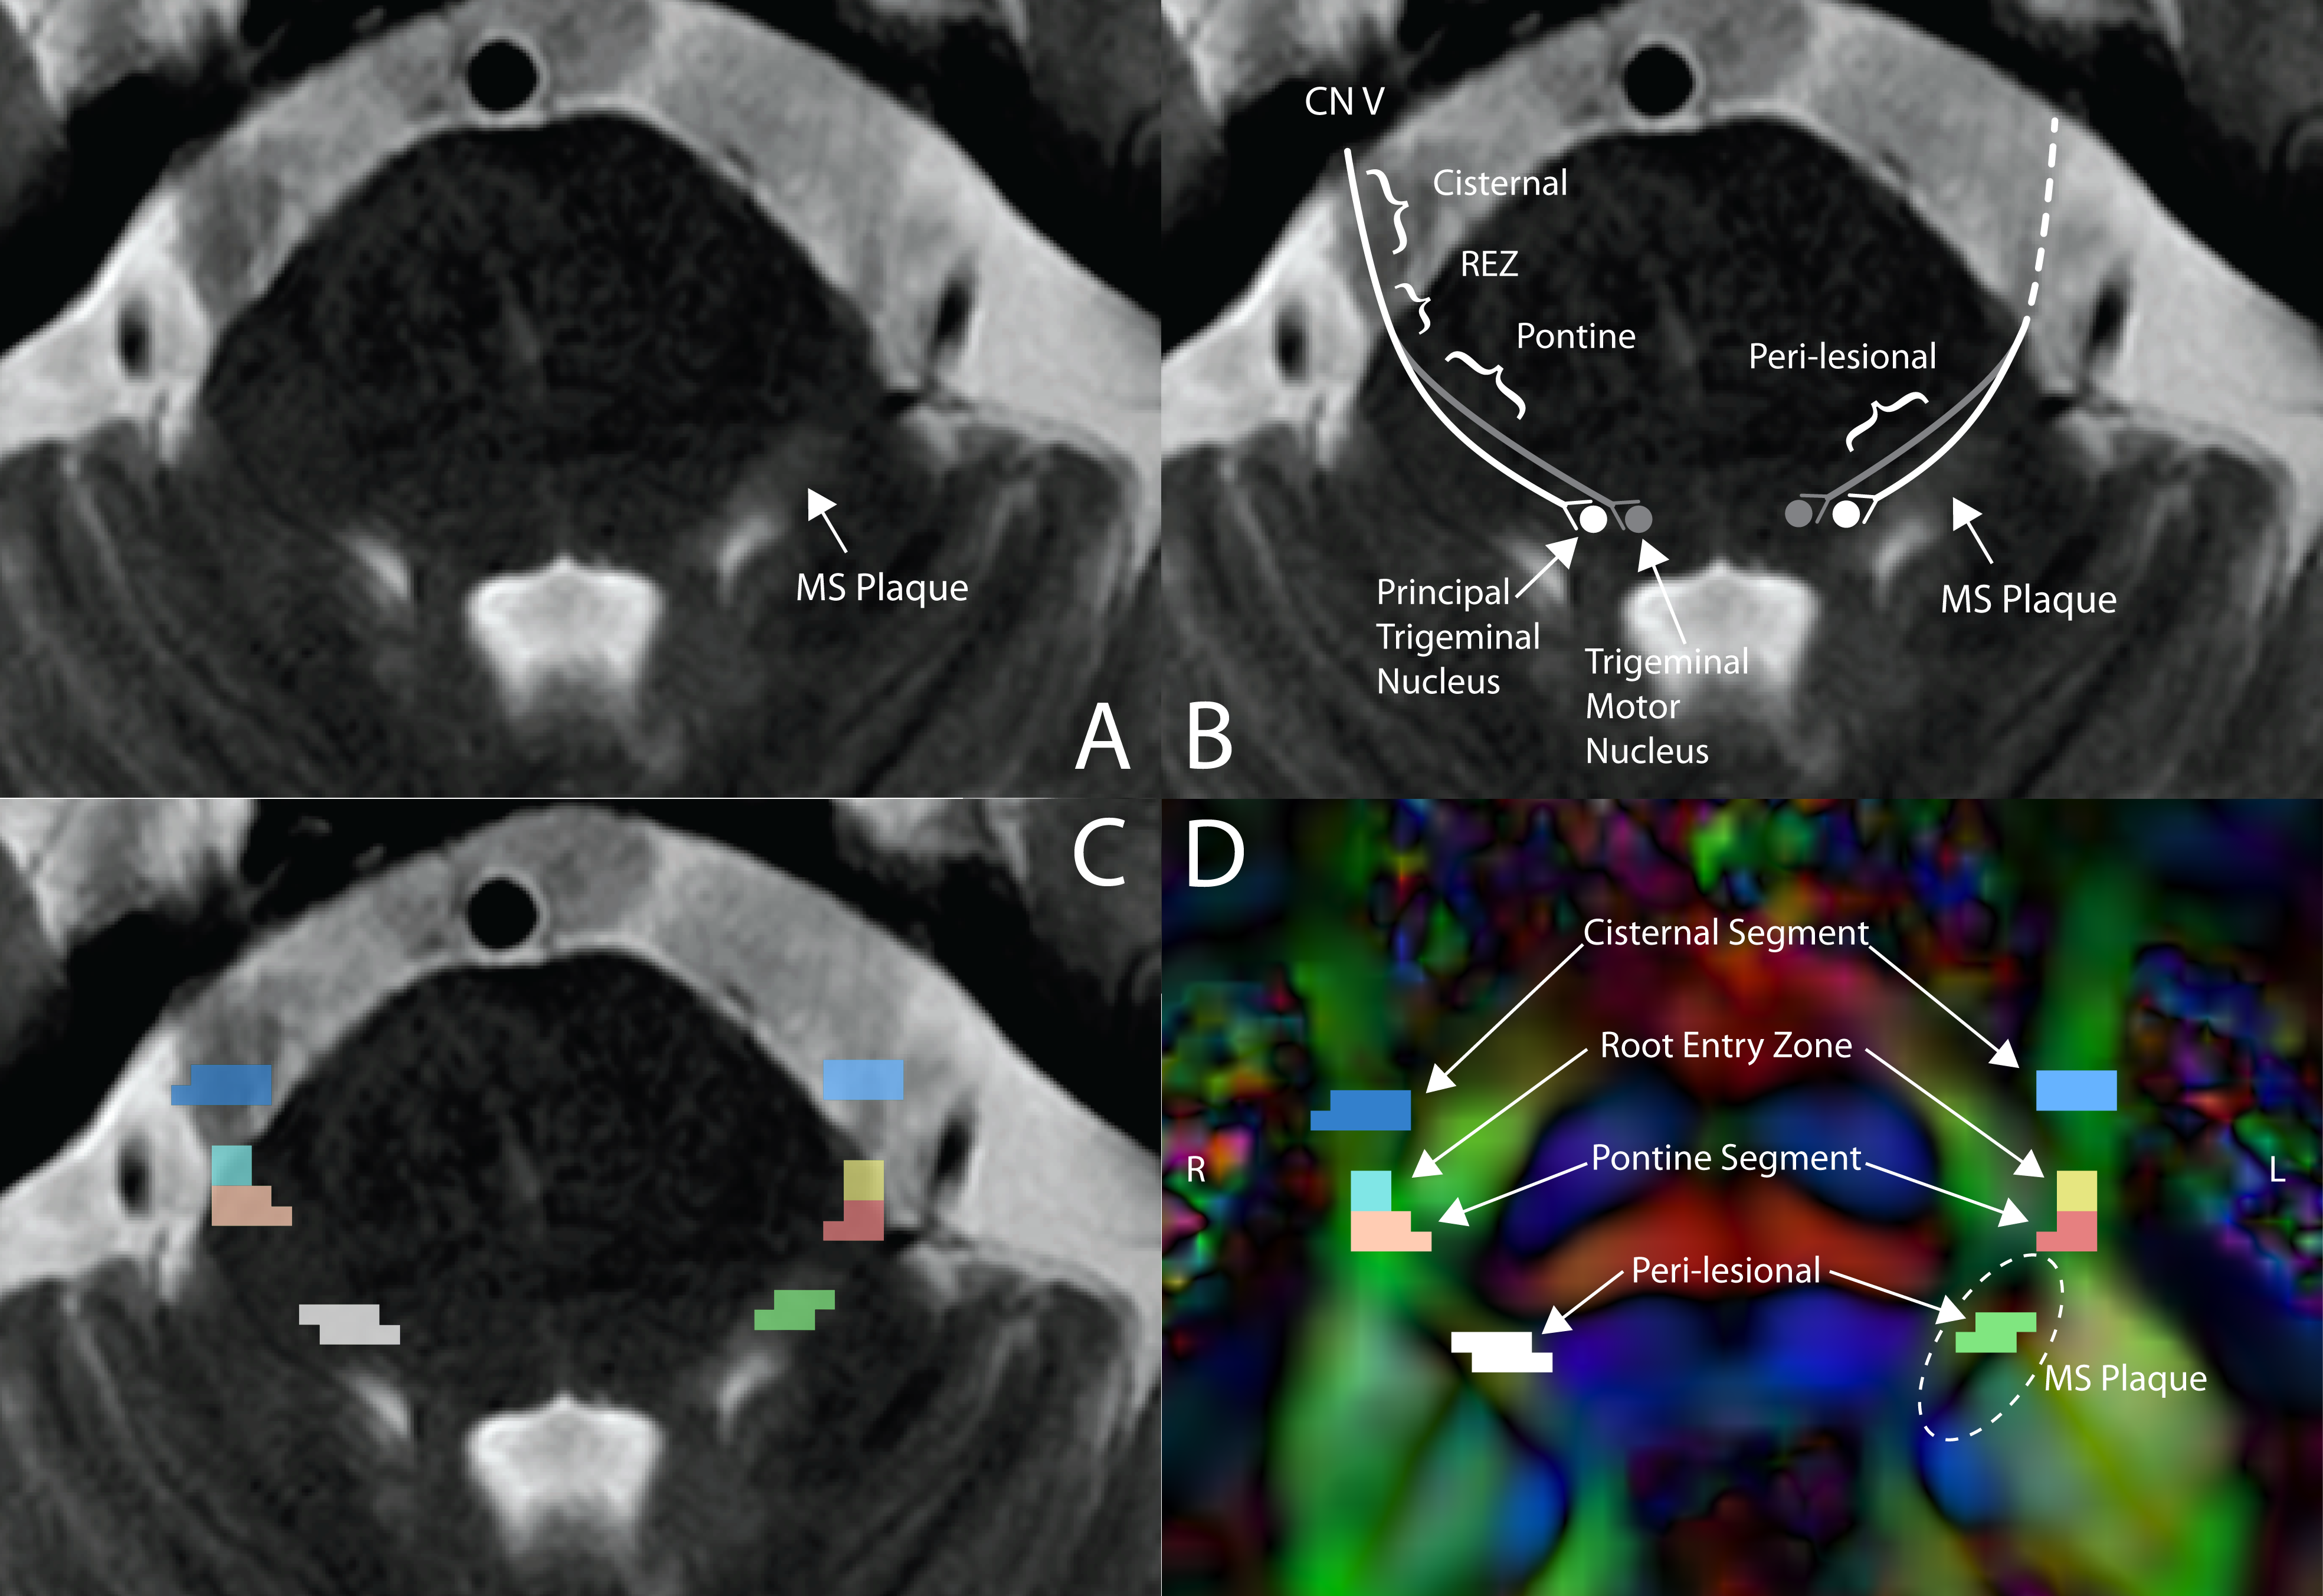
\includegraphics[width=\textwidth]{figure1.png}
\caption{Figure shows the MR images of a typical MS-TN patient at the level of pons. The presence of MS plaque in the CNS at the level of trigeminal nerve is characteristic of MS-TN (panel A). Panel B shows the expected course of the trigeminal nerve (CN V) as it synapses onto the principal trigeminal and motor trigeminal nuclei. Note that the exact anatomical relationship between the MS plaque and CN V in this instance cannot be clearly discerned in T2 due to the lack of contrast between the nerve and the surrounding tissue (panels A,B,C). Panels C and D show the placements of the ROIs along the CN V nerve bilaterally in order to measure diffusivity statistics, overlaid with the axial anatomical/ DTI image. The colors of the DTI image are rendered as color-by-orientation, where by convention red represents left–right, greens represents anterior–posterior and blue represents inferior–superior orientations. Diffusion statistics were measured from four groups of regions: cisternal segment, root entry zone (REZ), pontine, and peri-lesional, as illustrated. Analogous regions in TN patients and controls were similarly placed. Care was taken to differentiate pontine and peri- lesional ROIs in order to measure lesioned and unlesioned regions.}
\centering
\label{fig:MSfigure1}
\end{figure}


\section{Results}
\subsection{MTT permits visualization of brainstem trigeminal fibres}
MTT allowed for the visualization of brainstem CN V fibres in isolation, by distinguishing them from the surrounding crossing cerebellar peduncular fibres. The SDT method could not adequately delineate the nerve (Figure 2). Comparison of tractography results between SDT and MTT showed that SDT was unable to differentiate fibres crossing the cerebellar peduncle fibres, while MTT delineated the brainstem course of CN V into the region of the trigeminal main sensory nucleus. Delineation of MS-TN CN V by MTT revealed that the tracts became visibly sparse as they came into proximity of the MS plaque (Figure 3A). FA decreases in proximity to the MS plaque could also be visualized by colour shift in the tractography model with more orange/yellow colour presented. The fibres of the unaffected CN V did not exhibit this change, and extended caudally into the trigeminal nuclei (Figure 3B). 

\begin{figure}[p]
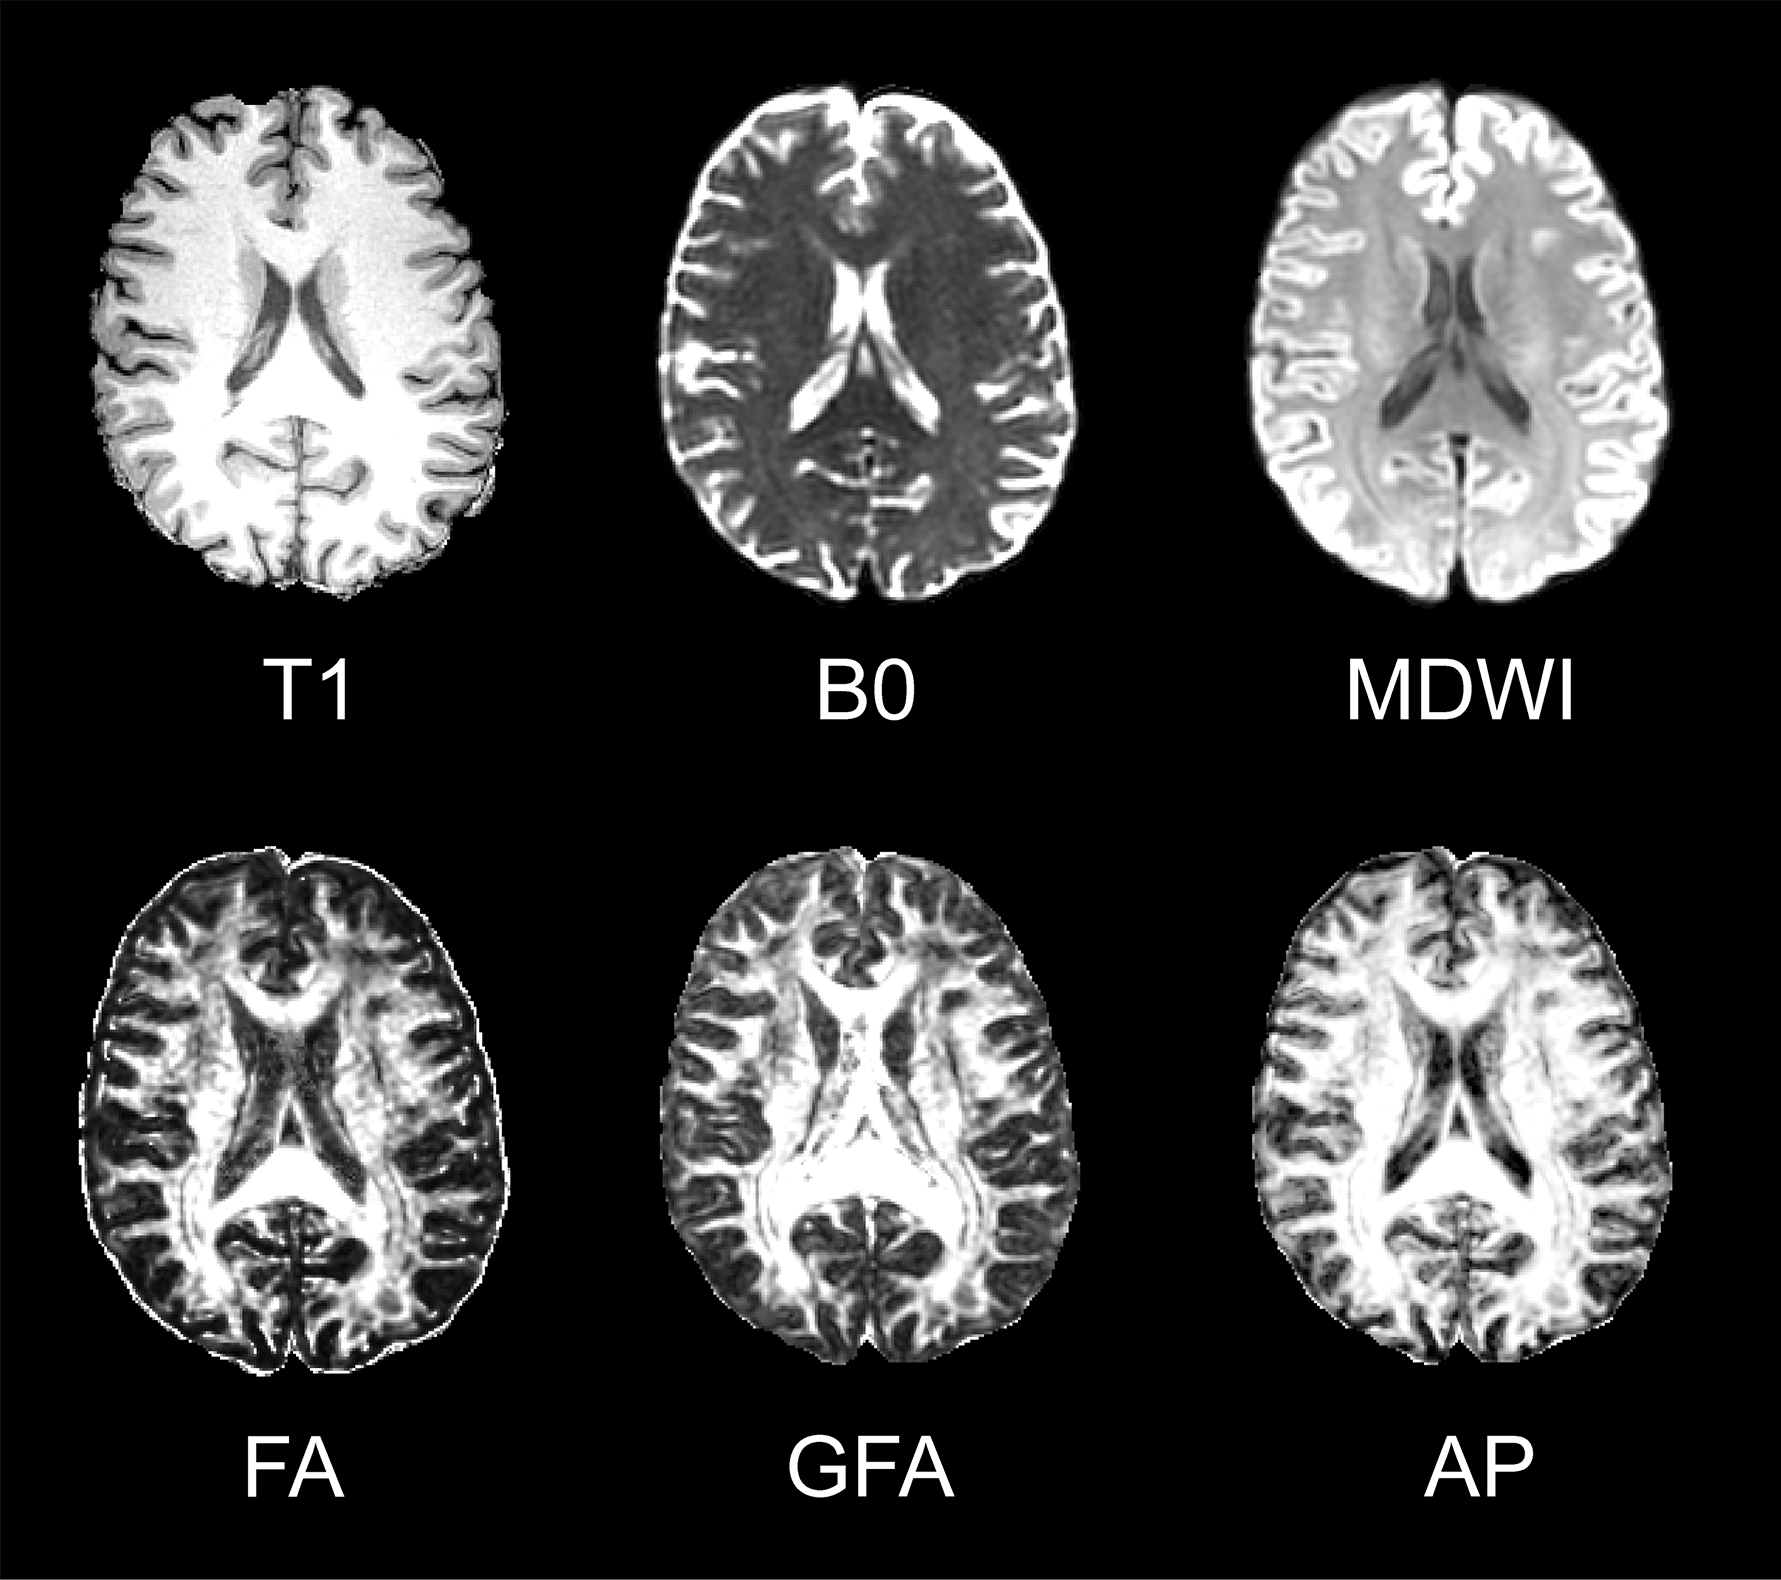
\includegraphics[width=\textwidth]{figure2.png}
\caption{Reconstruction of the trigeminal nerves at the level of pons from a single healthy subject in superior axial views. The reconstructed tracts are overlaid onto the axial DTI/anatomical images. The colors of the underlying scan are rendered as color-by-orientation, where by convention red represents left–right, greens represents anterior–posterior and blue represents inferior–superior orientations. The colors of the tractography fibers represent the spectrum values of FA (0 to 1), as shown by the legend at the top right corner. Panel A shows that SDT tractography delineated the cerebellar peduncle fibers, but cannot distinguish the brainstem trigeminal fibers (yellow arrows). Red arrows denote the starting point of tract generation for both SDT and MTT methods. Panel B shows that MTT tractography visualized CN V as it coursed through the brainstem towards the trigeminal main sensory nuclei (yellow arrows).}
\centering
\label{fig:MSfigure2}
\end{figure}

\begin{figure}[p]
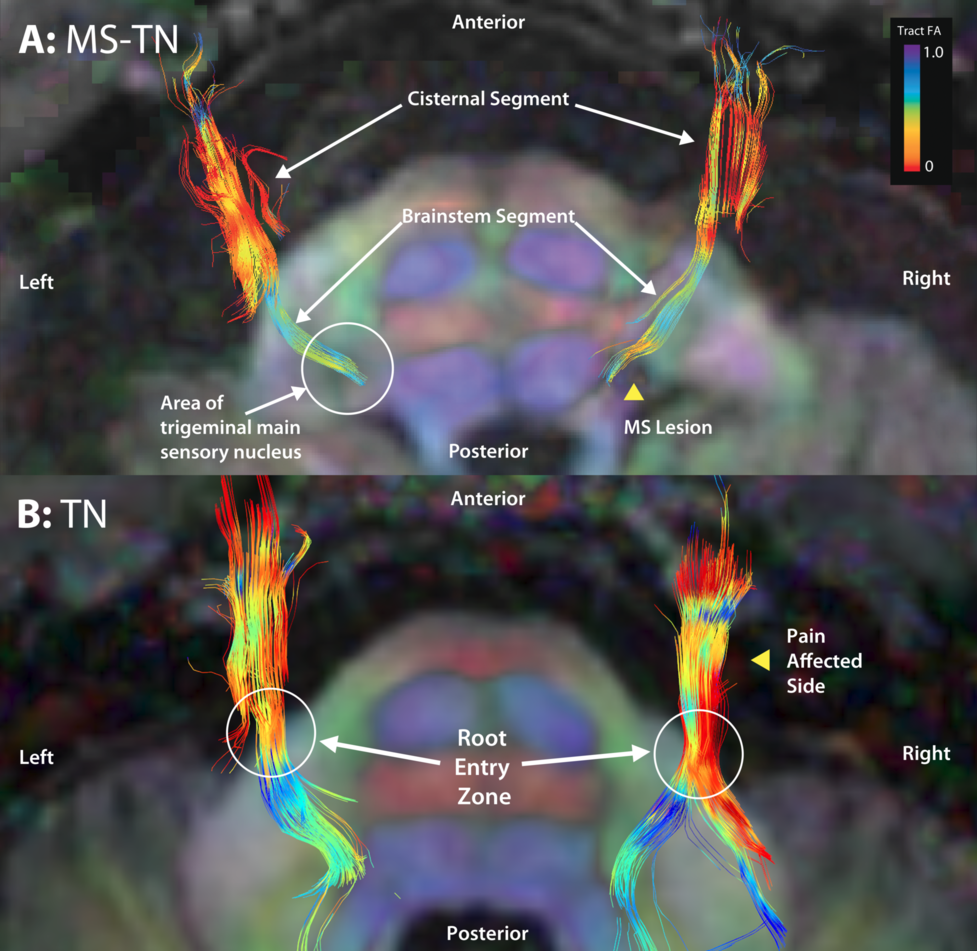
\includegraphics[width=\textwidth]{figure3.png}
\caption{Comparison of tractography delineation between affected and unaffected CN V nerve in the region of the trigeminal main sensory nucleus using the MTT method. Images are shown in superior axial view. Panel A shows the MS-TN tractography delineations. There is focal decrease in CN V FA in the region of the MS lesion (yellow arrow). Panel B shows the TN tractography delineations, where there is no such FA decrease in the brainstem segment. Please refer to Figure 2 for explanations of color scales and figure annotations.}
\centering
\label{fig:MSfigure3}
\end{figure}


\subsection{TN and MS-TN are characterized by specific diffusivity signatures}
The resulting coefficient matrices demonstrated unique patterns of diffusion metrics across subject groups in each of the CN V segments measured. Each nerve segment is studied separately, and differences in regional diffusivities were examined in both intra-subject comparisons between symptomatic and asymptomatic sides, as well as inter-subject comparisons between subject groups. The details of the examinations are described as follows:

\subsubsection{Cisternal changes are unique in TN}
In the cistern segment (Figure 4), statistically significant differences are found only between the TN group and other groups. No significant differences were found in between segments of other subject groups. Specifically, the FA measure of symptomatic side (+) in TN patients is shown to be significantly greater compared to all of the other patient groups and segments, while the asymptomatic side (-) in TN patients does not show any significant differences compared to other groups. In RD, AD and MD measurements, the only significant differences are observed between TN(+) and TN(-), where TN(+) RD/AD/MD are lower than that of TN(-). No symptomatic/asymptomatic (+/-) or left/right differences were observed in MS-TN and control groups. These results suggest that the cisternal CN V diffusivity changes are unique to the TN group. 

\subsubsection{REZ changes are found predominantly in TN}
In the REZ (Figure 5), statistically significant results are found within, but not unique to TN. TN(+) FA is shown to be significantly lower than TN(-) FA, while TN(+) RD and MD are shown to be significantly greater than TN(-); TN(+) MD and RD are shown to be significantly greater compared to all other groups and sides; while TN AD showed no significant differences. In contrast, MS-TN patients showed no significant differences between MS-TN(+) and MS-TN(-) sides in any of the diffusivity metrics, suggesting no intra-group differences. Comparisons between MS-TN(+/-) and TN(+/-) revealed no significant inter-group FA differences. However, both TN and MS-TN groups are shown to be different from controls. Both TN(+/-) and MS-TN(+/-) REZ have significantly lower FA than that of control REZ; control AD and RD are shown to be significantly lower than TN(+/-); while there is no significant difference between left and right sides in controls. 
\subsubsection{Pontine diffusivities showed no significant changes in all groups}
In the pontine tissue (Figure 6), there are no significant intra-group or inter-group differences in FA, RD and MD for all groups and sides. However MS-TN(-) AD is significantly higher than TN(+/-) and controls. No intra-group AD differences were found in MS-TN.
2D. Diffusivities in peri-lesional trigeminal fibres highlight MS-TN pain

In the peri-lesional region (Figure 7), the patterns shows significant intra-group and inter-group differences in MS-TN. MS-TN(+) FA is significantly lower than that of MS-TN(-), as well as significantly lower than TN(+/-)and Controls, while MS-TN(-) FA showed no inter-group differences with TN and Controls. RD, and MD showed only intra-group differences between MS-TN(+) and MS-TN(-),where MS-TN(+) RD and MD are significantly higher than that of MS-TN(-). AD showed no significant differences. The pattern of differences for peri-lesional region is unique to MS-TN. 

\begin{figure}[p]
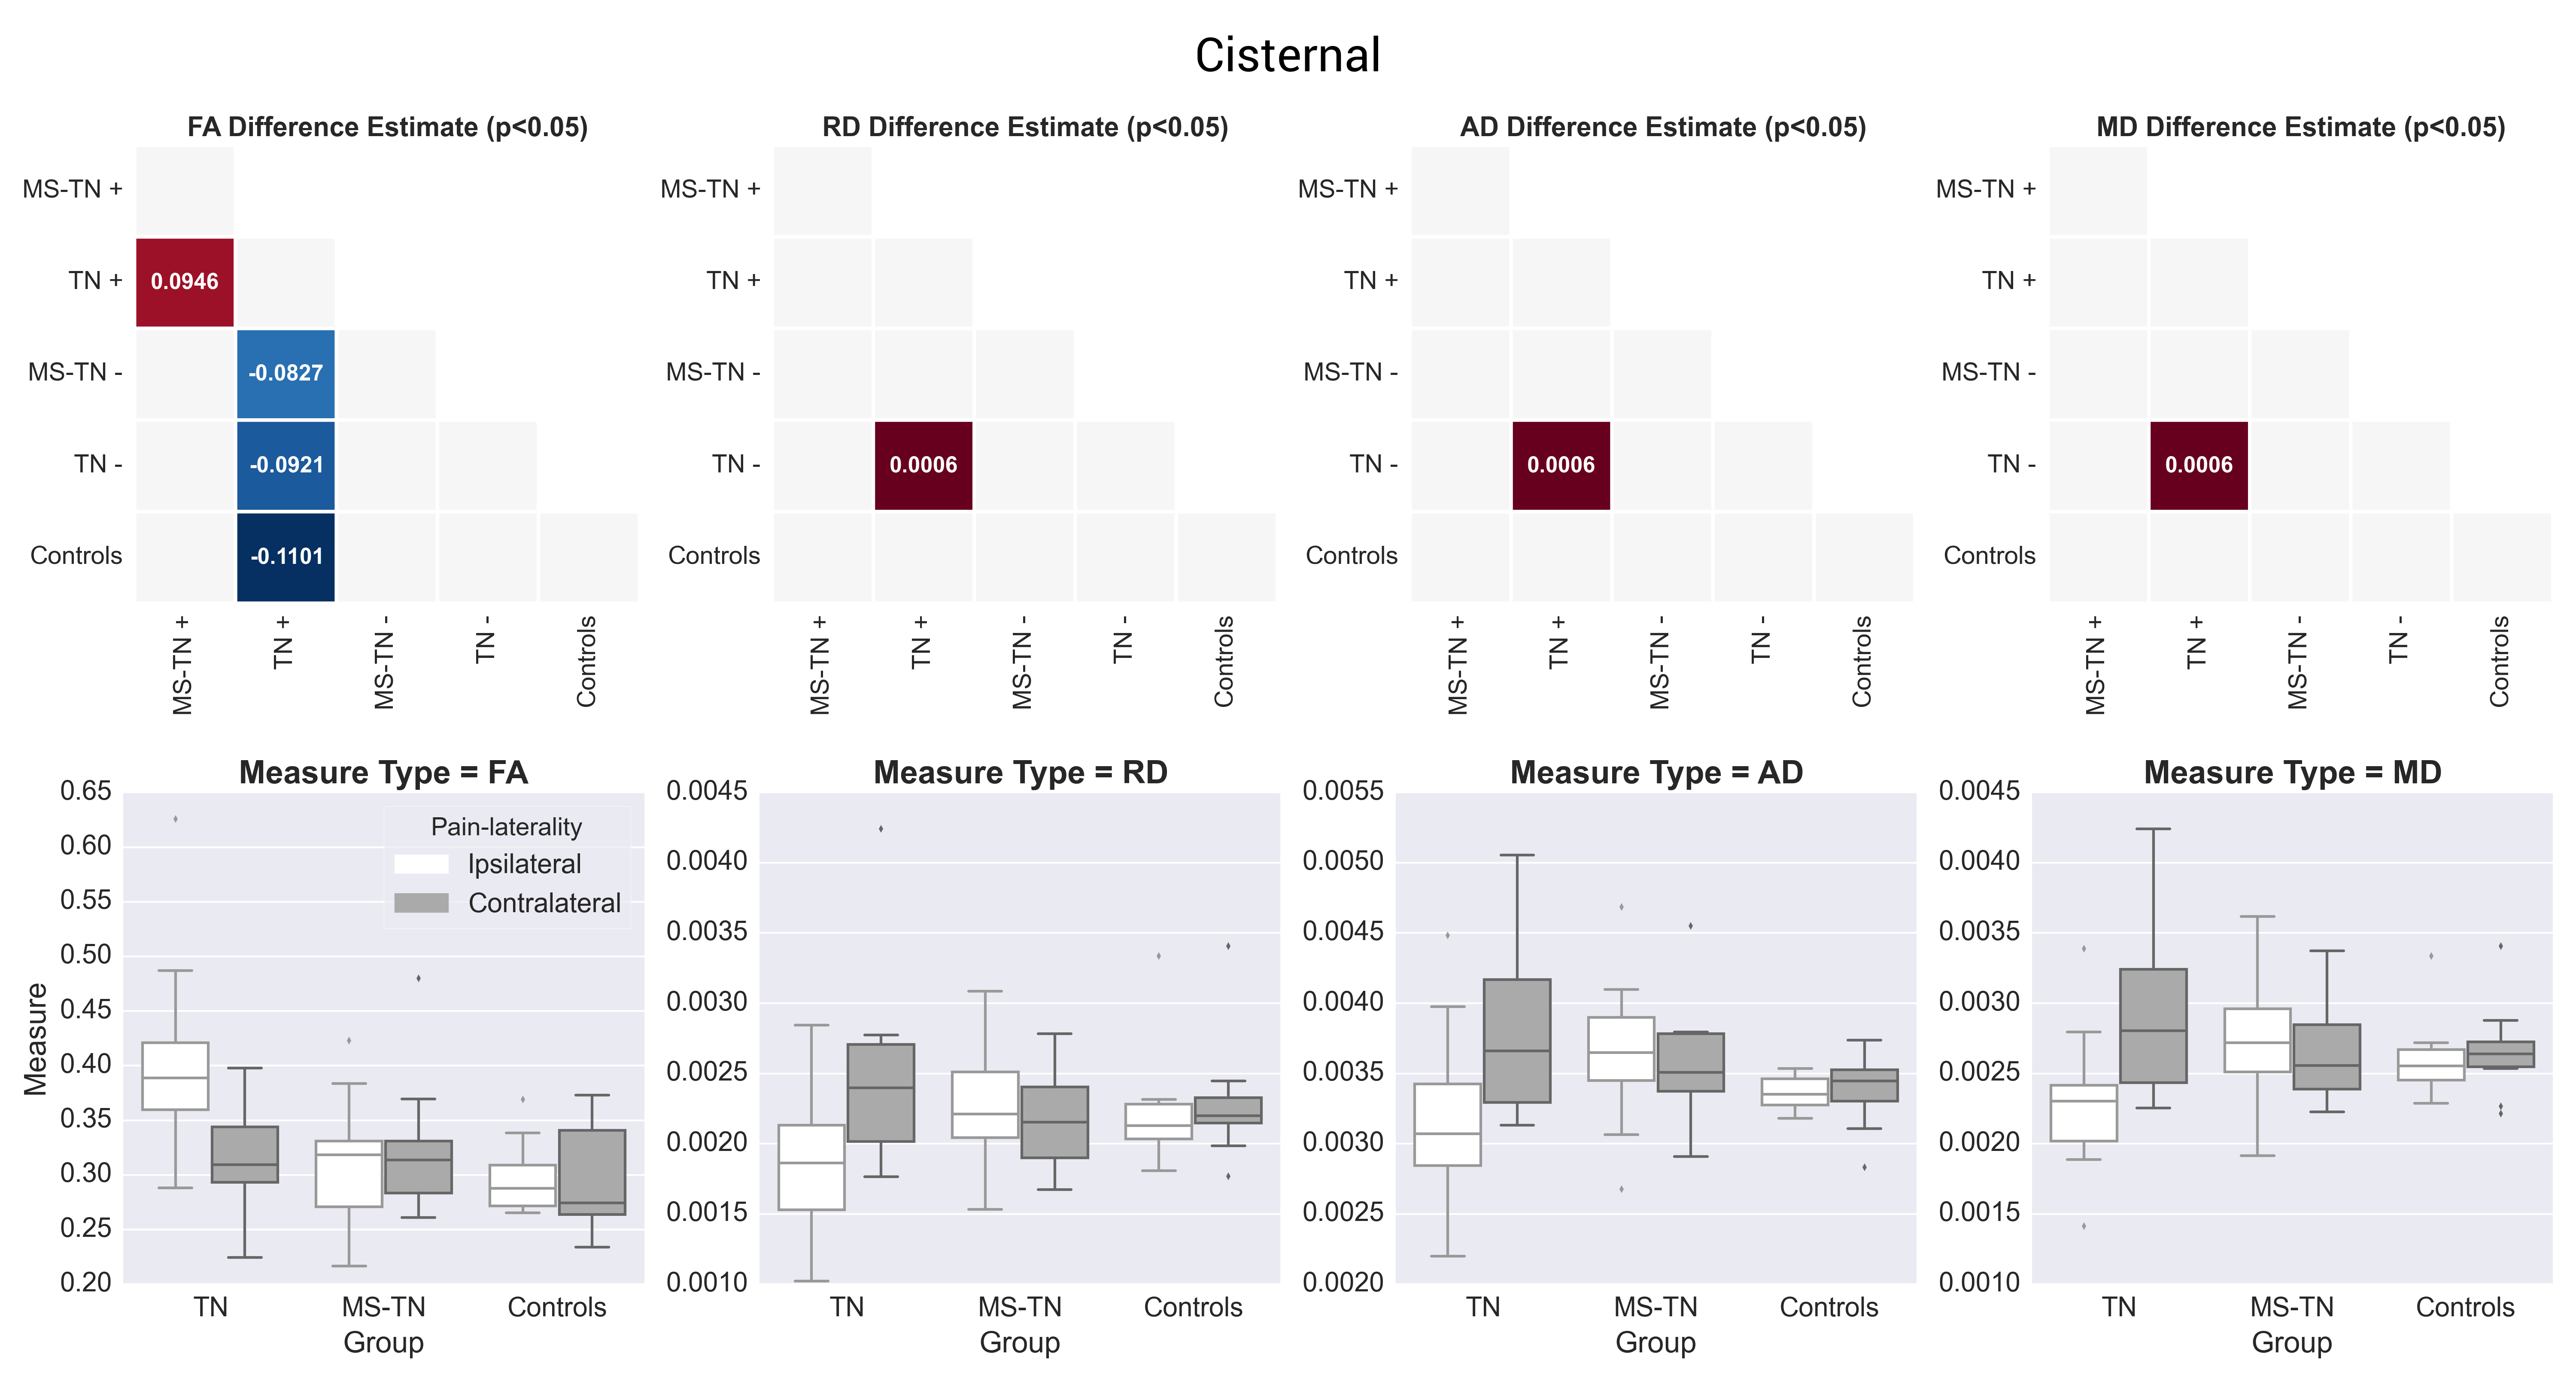
\includegraphics[width=\textwidth]{figure4.png}
\caption{Top row: Diffusivity difference estimate matrices of the Cisternal ROIs demonstrating significant differences in regional diffusivities between MS-TN patients, TN patients and controls. Colored squares indicate statistically significant differences (p\textless 0.05) after correcting for multiple comparisons with false discovery rate. The (+/-) sign indicate symptomatic (+) and asymptomatic (-) sides of the subject group. The matrix should be read as ‘Y axis in relation to X axis’—for example, A red square indicates that the vertical axis measure (e.g. TN+, the affected side in TN patients) is significantly higher than that of the horizontal axis measure (e.g. MS-TN+, the affected side in MS-TN patients); blue indicates that the measure is lower. The number within the square indicates relative estimated differences. Bottom row: Box-plots of the diffusivity distributions. Note that the control group does not have pain lateralities, therefore ipsilateral indicate the right side in the control group in this figure. The mean of the left-right diffusivities in controls were used for comparisons against other groups. The analysis highlights TN+ specific diffusivity differences in the Cisternal segment of the trigeminal nerve. Specifically TN+ has significantly higher FA than all the other groups, and that there are significant differences between TN+ and TN-. The points above and below the box plots are outliers. Significances are not indicated in the plot, for pair-wise significance, please refer to the estimate matrices above row.}
\centering
\label{fig:MSfigure4}
\end{figure}

\begin{figure}[p]
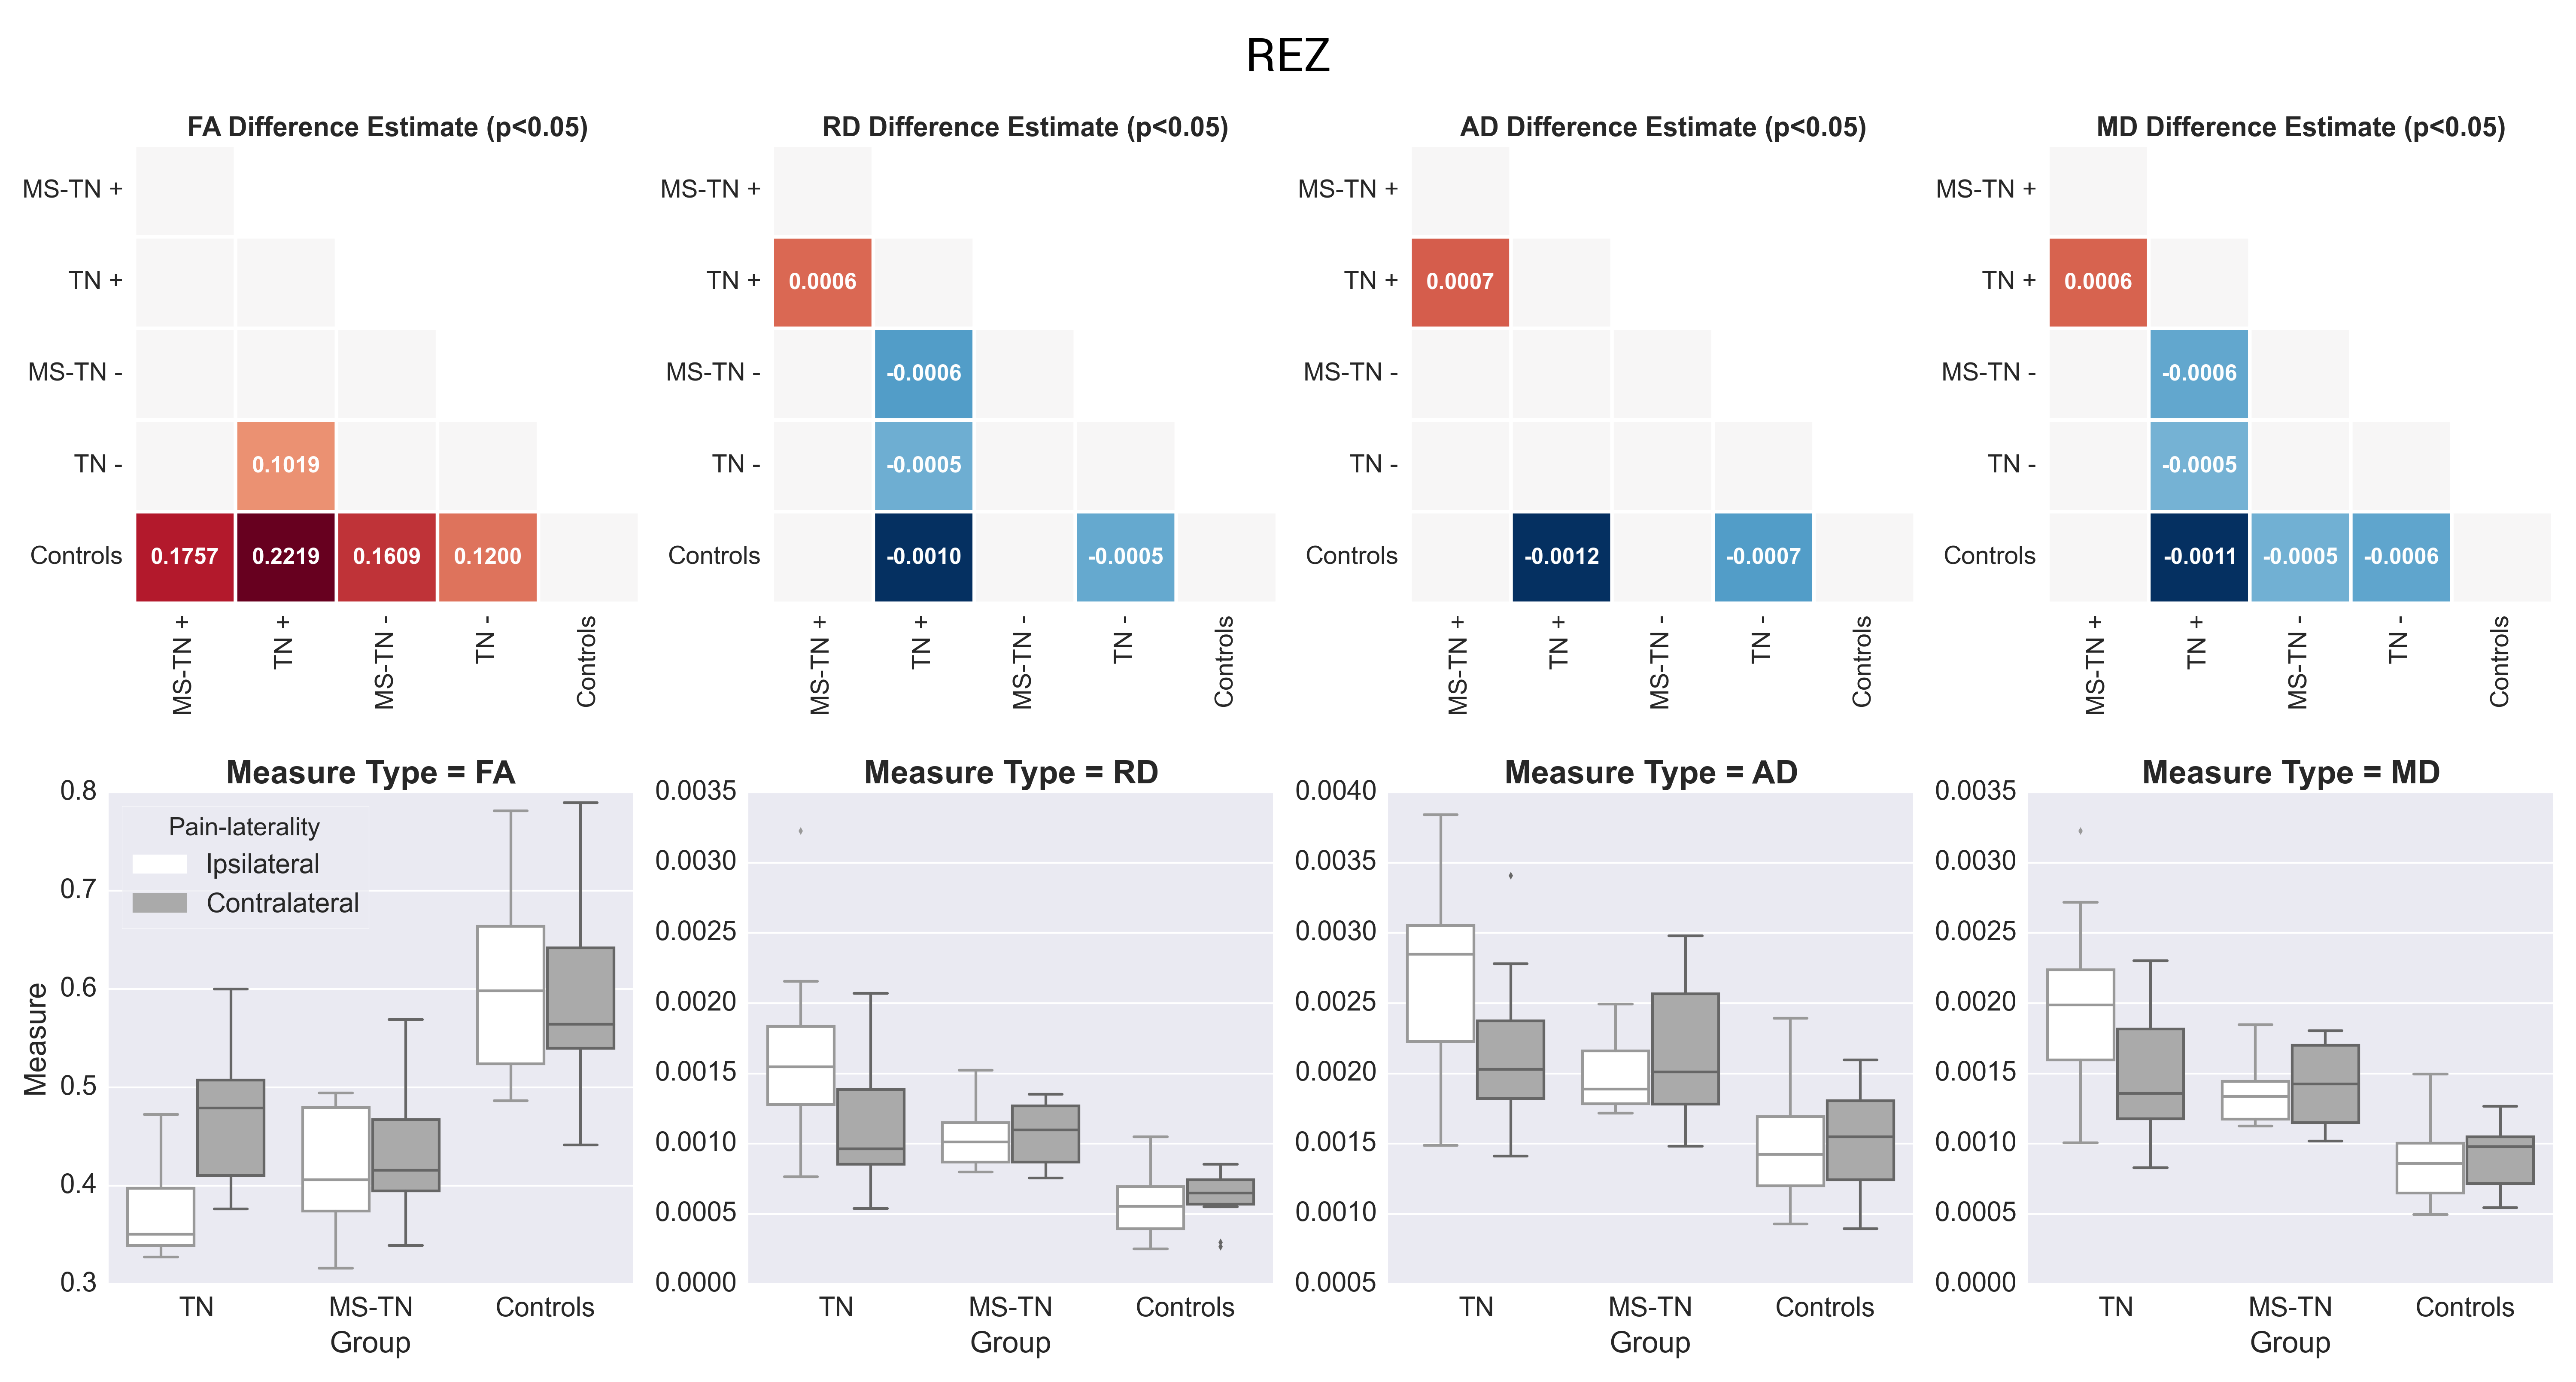
\includegraphics[width=\textwidth]{figure5.png}
\caption{In the REZ, MS-TN, and TN patients have significantly different diffusivities when compared to controls. TN+ also shows significantly different FA, RD, and MD from TN-. Moreover TN+ shows significant different from MS-TN+ as well. Please refer to Figure 4 for explanations of layout and annotations.}
\centering
\label{fig:MSfigure5}
\end{figure}

\begin{figure}[p]
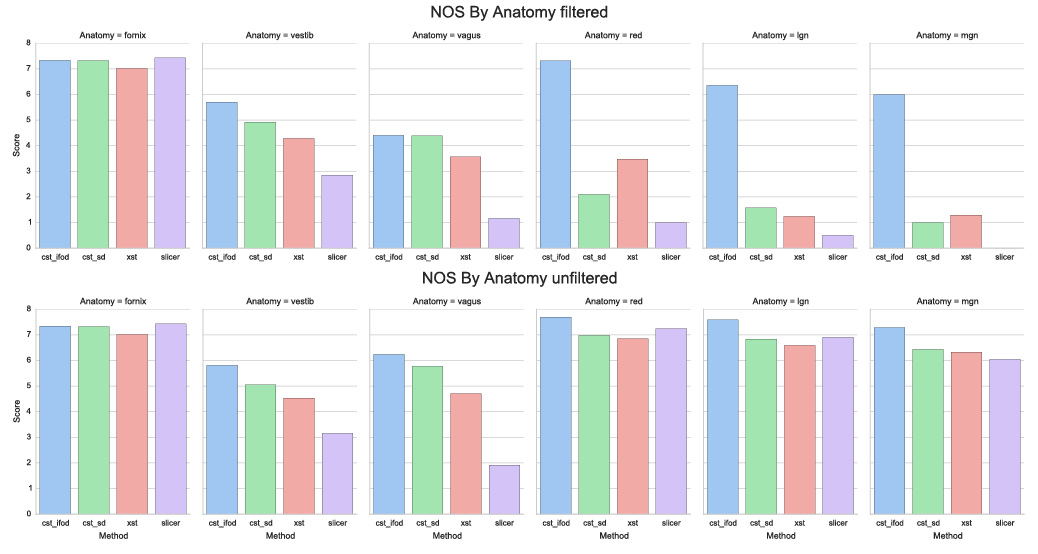
\includegraphics[width=\textwidth]{figure6.png}
\caption{In the pontine segment unaffected by MS plaques, there are little differences between groups. However MS-TN- shows significantly different AD than TN- and controls. Please refer to Figure 4 for explanations of layout and annotations.}
\centering
\label{fig:MSfigure6}
\end{figure}

\begin{figure}[p]
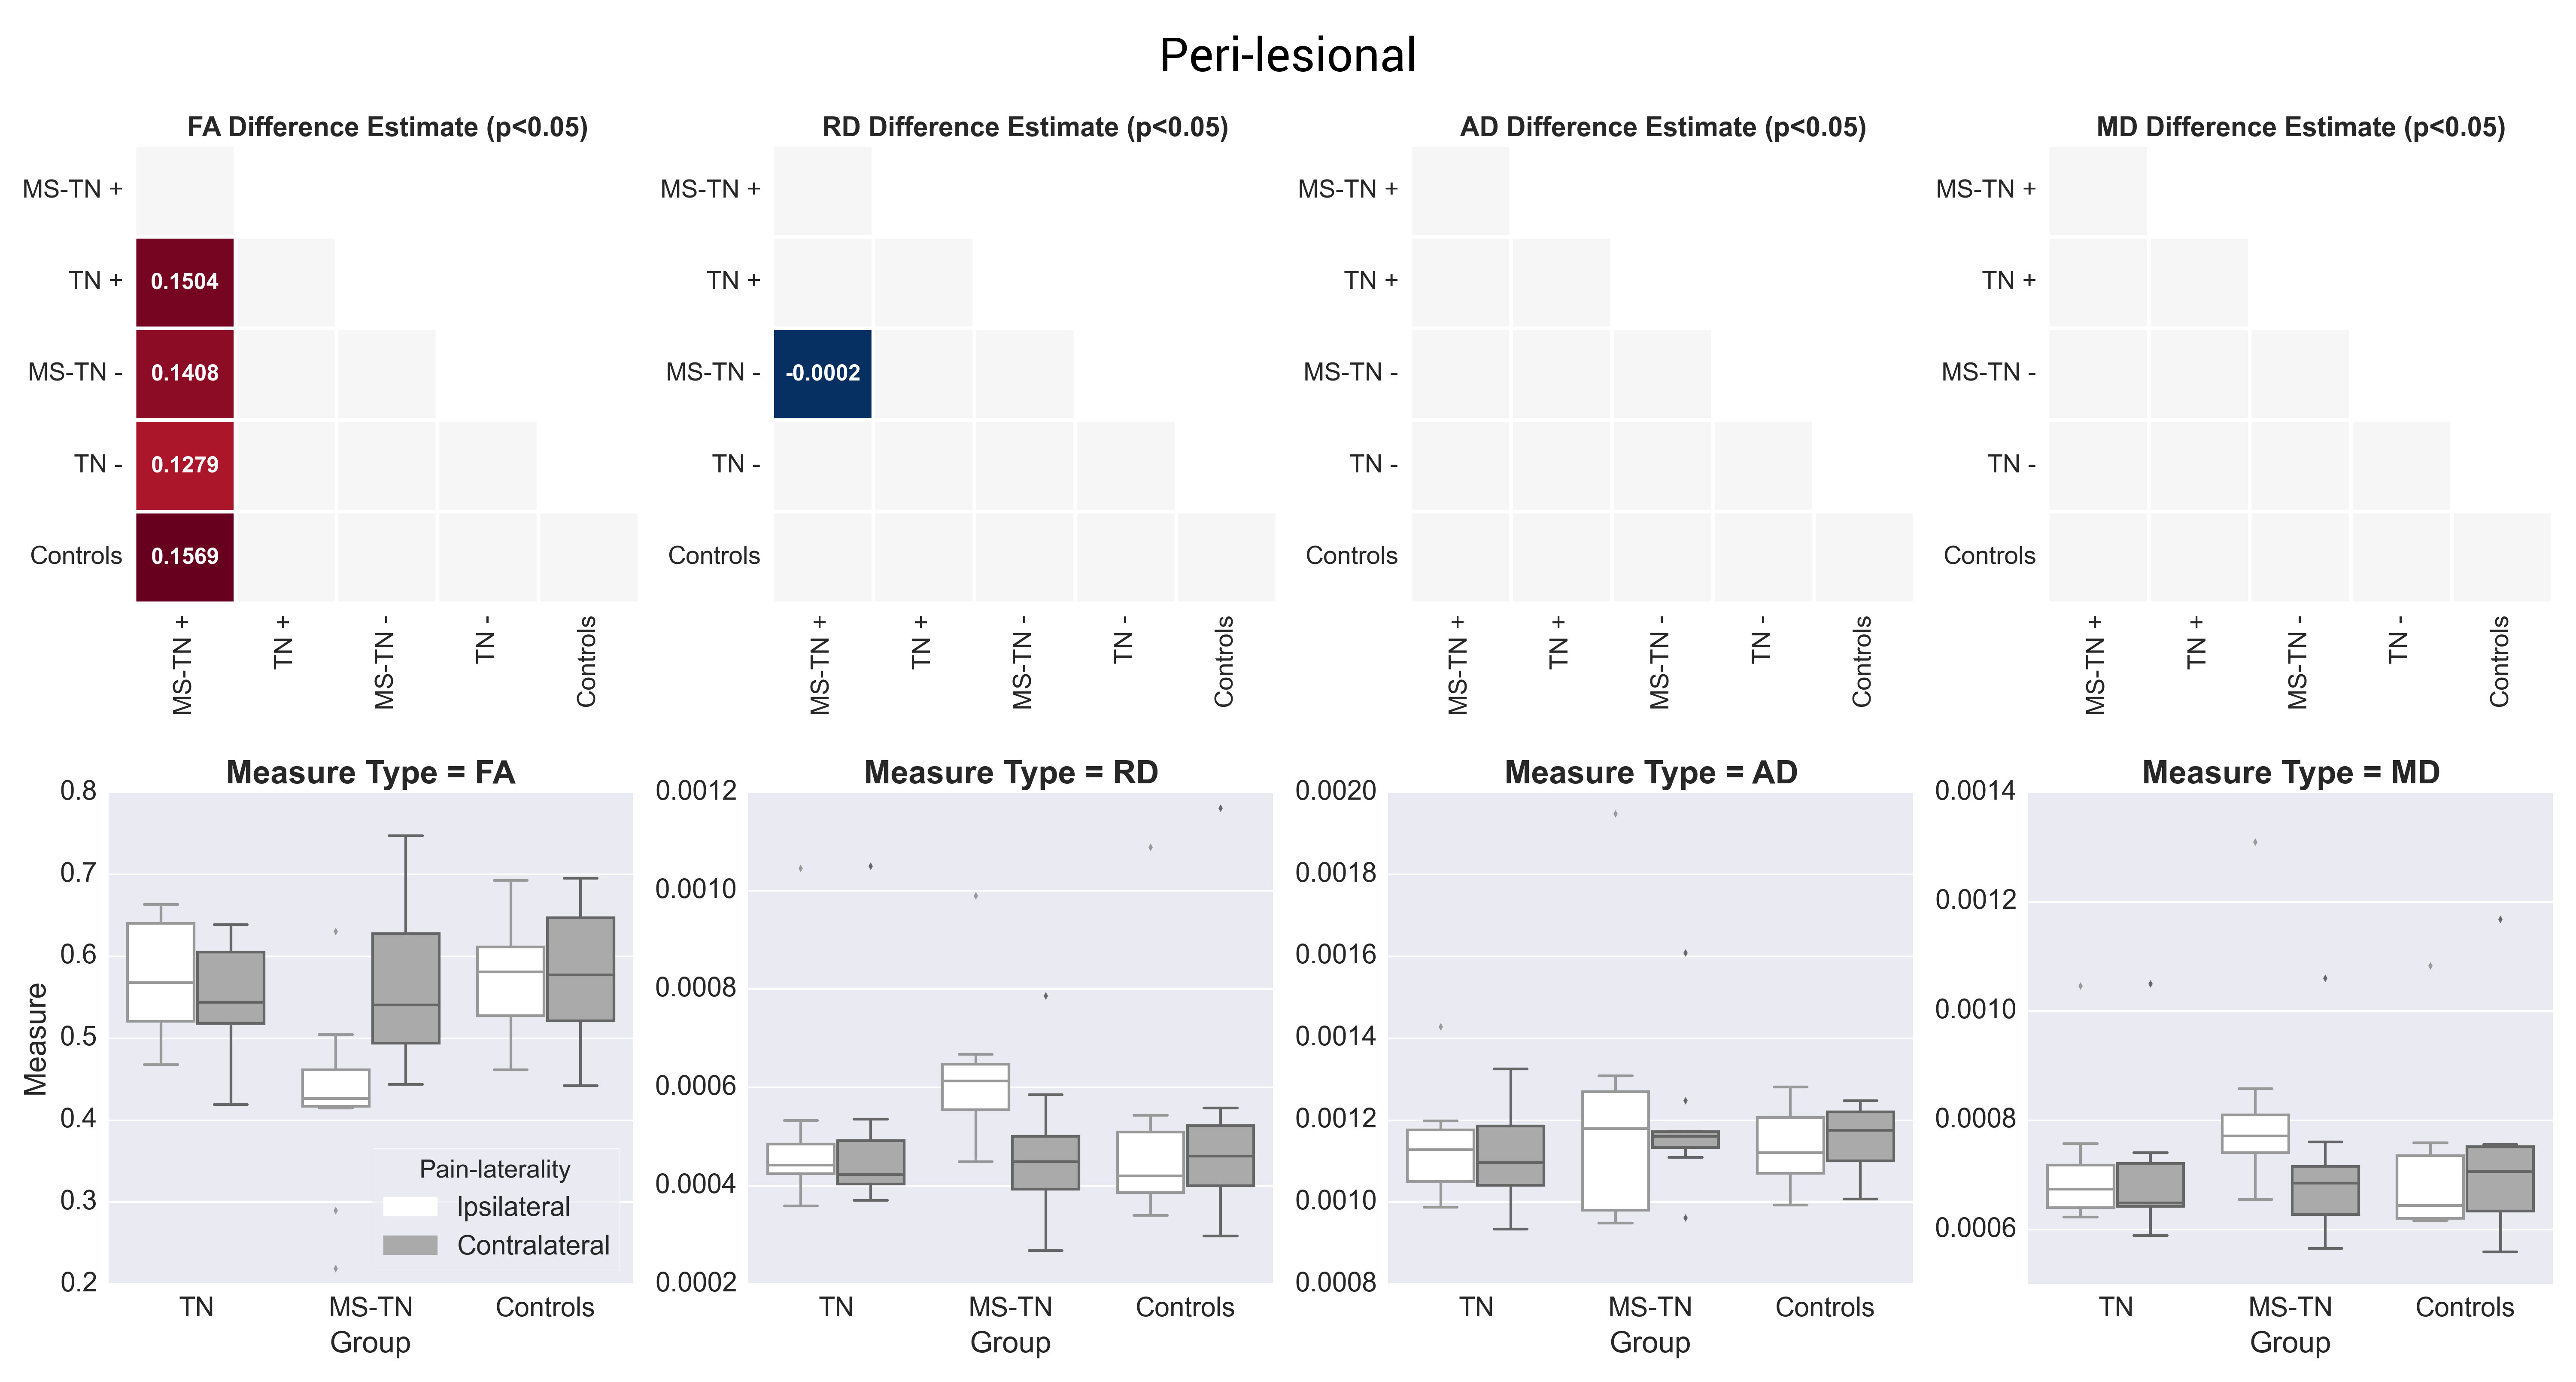
\includegraphics[width=\textwidth]{figure7.png}
\caption{The peri-lesional segment highlighting MS-TN+ specific diffusivity differences. Both MS-TN+ and MS-TN- show significantly lowered FA than all the other groups. RD of MS-TN- is also significantly lower than that of MS-TN+. Please refer to Figure 4 for explanations of layout and annotations.
http://msj.sagepu}
\centering
\label{fig:MSfigure7}
\end{figure}

\section{Discussion}

We demonstrate for the first time that diffusion MRI tractography is capable of anatomically distinguishing between TN and MS-TN. Analyses revealed unique, focal MS-TN diffusivity changes along CN V. These changes highlight the differences in diffusivities between MS-TN, TN and healthy controls, thereby permitting their use as neuroimaging signatures for distinguishing these conditions. 
Previous studies of the CN V with DTI tractography have been met with limitations of the single-tensor Gaussian diffusion model, and were incapable of resolving brainstem trigeminal tracts (Figure 2A). Recent improvements in multi-tensor imaging are now capable of more complex diffusion profile of crossing fibres in neural tissue, thereby permitting reliable reconstruction of the brainstem CN V (Figure 2B), and subsequently the study of CN V changes in MS patients (Figure 3). 

In patients with MS-TN we expected no changes in the extra-axial CN V segment, and that adverse changes to the CN V would be found in the intra-axial segment, within close proximity to the MS lesions. Conversely in TN patients, we expected CN V changes to be found within or near the extra-axial segment due to neurovascular compression. 

The results have agreed with our initial hypothesis. The coefficient matrices (Figures 4-7) revealed specific patterns demonstrating TN-specific diffusivity changes in the cistern and MS-TN-specific changes in the peri-lesional regions. In the TN REZ, FA changes are similar to the results found by DeSouza et al (Desouza, Moayedi, Chen, Davis, \& Hodaie, 2013; DeSouza et al., 2014), where the FA of the TN(+; pain-affected side) CN V is lower than that of TN(-; non-affected side). Additionally, while RD and MD changes in the TN REZ showed significant differences, no AD differences in the REZ were detected, suggesting that the nature of the diffusivity changes may be due to demyelination of the central myelin within the REZ. Interestingly, the cisternal TN(+) FA is demonstrably higher than the TN(-) segment, and also the cisternal FA of all other groups, suggesting that cisternal and REZ FA changes in TN are not homogenous along the nerve segment. Although there has been reports of hyperintensities in the cisternal CN V T$_{1}$ image with gadolinium contrast in MS \cite{VanderMeijs2002}, the lack of MS cistern findings in this study may be due to the limit of the sampled MS population. MS plaque locations are highly variable, and MS-TN patients were not filtered specifically for cistern region plaques. 

Diffusivity disruptions of CN V in MS-TN patients are likely due to MS plaques at the regions proximal to the main sensory nucleus. While AD has been associated with neurological disruptions in MS\cite{Budde2009,Kim2006}, the present study showed a lack of change in AD. This may relate to the observation that we did not select subjects based on their disease severity, but based on their pain. Disease severity was in fact variable in this group. Future studies will be able to address this point in more detail, by taking into account other MS manifestations in addition to pain, and correlation with diffusion metrics. Lower REZ FA in MS-TN compared to controls suggests that global neural tissue diffusivity in MS-TN is significantly different from that of healthy controls. Similar findings can be seen in the pontine region, where only the MS-TN AD measures are distinctly different from the other groups. However while AD is commonly correlated with axonal integrity, the high concentration of crossing fibers in the pontine region may introduce confounds into these correlations. Improvements in diffusivity metric measurements in such tissues are needed to further understand these findings. 

\subsection{Limitations and future directions}
The study aimed to demonstrate that diffusion MRI can detect localized CN V differences in MS-TN, and to evaluate the feasibility of this novel approach in a group of patients. Therefore we did not explore the course of MS disease progression and other details in the MS-TN patient group in this study. However it has demonstrated that by utilizing MTT to not only visualize, but also to assist in nerve segmentation and statistical analysis, more complete insights into the changes of white matter anatomy can be gained. We have found that peripheral CN V does not change homogeneously in pathology. Other white matter pathways are also likely to be differentially affected in varying segments in other pathological states such as MS. 

With this approach, future longitudinal studies may reveal more about white matter changes and associated pain, cognitive, and motor-related measures across the disease’s progression. Moreover, this strategy may allow for pre- and post-treatment predictions in white matter changes, ultimately aiding in clinical prognostication and the identification of high-risk subjects. Therefore, this study paves the way for a more systematic approach to the understanding of pain and white matter anatomy using non-invasive neuroimaging techniques.

\section{Conclusion}
The study demonstrates that MS-TN and TN have differentially localized pathophysiology at the level of CN V in the brainstem. MS plaques disrupt the diffusivity of brainstem CN V fibres near the CN V nucleus, while TN diffusivity disruptions are focused on the cistern and REZ segments. The regions affected by MS and TN REZ suggest changes in myelination of the affected CN V segment. Using this imaging technique, TN and MS-TN can be distinguished by unique localized diffusivity changes in the different CN V segments.
\graphicspath{{images/ap-reg/}}

\chapter{Study II: Diffusion Weighted Image Co-registration: Investigation of Best Practices}
\chaptermark{Study II}
\label{section:study2}

\bibentry{Chen2018ap}

\section{Abstract}

\textbf{Purpose:} The registration or alignment of diffusion weighted images (DWI) with other imaging modalities is a critical step in neuroimaging analysis. Within-subject T1-DWI co-registration is particularly instrumental, although DWI acquisitions are susceptible to linear and non-linear field distortions, and it becomes even more important with increasing dataset size. DWI-derived scalar images are commonly used as intermediates for T1-DWI co-registration, and the resulting registration transforms are applied to all other scalar images for analysis. The ideal registration intermediate should register well to T1 and other multimodal images and be practically easy to obtain. It is however, currently unclear which DWI-derived scalar image serves as the best intermediate. We aim to determine the best, practical, intermediate for image co-registration. 

\textbf{Methods:} T1 and DWI images were acquired from 20 healthy subjects. DWIs were acquired with 60 directions.  Six DWI-derived scalar images were compared including: 1) fractional anisotropy (FA); 2) generalized FA (GFA); 3) B0 images; 4) mean DWIs with the B0 image (MDWI); 5) anisotropic power (AP) images. Registrations were performed using Anatomical Normalization Tools (ANTs) with affine registration and symmetric diffeomorphic registrations. Pair-wise log joint histograms of the DWIs were plotted to examine possible group biases. Mutual information (MI) and cross-correlation (CC) scores were used to measure the similarities between the deformed DWIs and T1 images. Percent change in these similarity scores relative to scores derived from the identity (baseline) transformation were used for comparison, with higher values indicating better registration.

\textbf{Results:} AP showed the smallest variability in registration improvements across all the tested DWI derived scalar images, and show the highest average percent changes with CC registration cost function (CC=1.2\%, MI=15\%). In contrast, the FA and GFA transforms resulted in significantly poorer registration across DWI types. 

\textbf{Conclusions:} The AP image was the DWI-derived scalar image that provided the most consistent registration to all other images. Practically, it is generated easily and so could be implemented in basic and clinical research pipelines currently using other intermediates. Given these findings, it is recommended that AP images be used for T1–DWI co-registration, and that FA and GFA images in particular be avoided.

\section{Introduction}

Diffusion magnetic resonance imaging (dMRI) allows for visualization and quantification of the brain’s white matter by measuring the anisotropy of water molecules \cite{Lenglet2009f}. The resulting diffusivity parameters are used to infer white matter directionality which are visualized using diffusion tensor images \cite{Basser2002}. These form the basis of study for a wide range of disease processes \cite{Chen2016a,Ciccarelli2008,Hodaie2012g}. DMRI has become an essential tool in the in vivo analysis of brain white matter, particularly when used at the group level \cite{Chen2016} to compare diffusion metrics and to model white matter tracts using tractography \cite{Chen2016,Chen2015c,Hodaie2010}. An increasing number of neuroimaging techniques, including structural connectivity analysis, also depend on dMRI to segment white matter regions \cite{Moayedi2012a,McGrath2013,Wiech2014}. 

Image registration permits the transformation of different, individual, diffusion images into one brain template and allows for group analysis. This multi-step process involves the accurate co-registration of within-subject diffusion-weighted images (DWI) and anatomical T1-weighted (T1) images, followed by registration of between-subject T1s to create a common template. Individual T1 images typically serve as the intermediate space due to their high spatial resolution and low incidence of distortions \cite{Avants2009,Brown1992,Klein2009,Tustison2014}. The registration of T1s to DWIs is critical to ensure the validity, reliability, and interpretability of the final results (e.g., in correlating DWI data to other measures, and for use in group analyses e.g. \cite{Chen2016}. However, while T1 to DWI co-registration is a common procedure in neuroimaging studies, it is currently unclear which DWI-derived scalar image serves as the best intermediate. 

The greatest challenge of T1-DWI co-registration is that DWI acquisitions are susceptible to both affine/linear (i.e. eddy-current and head motion) and non-linear echo planar image field distortions \cite{Rohde2004}. The most common strategies to account for such issues include: 1) correcting all DWI distortions before co-registration with a T1 image, and/or 2) using non-linear co-registration transformations to best warp the anatomical image to DWI space. Corrections for DWI distortions generally involve affine registration of each of the diffusion gradient images to a non-diffusion-weighted image (B0), followed by a rotational correction of the original diffusion gradient b-matrix \cite{Leemans2009}. This approach, however, does not account for non-linear distortions, such as those typically found in the brainstem and frontal and temporal cortices, that are due to MRI field inhomogeneity. Affine co-registration of the T1 image directly to DWI results in poor and highly variable overlaps – increasing the likelihood of both type I and type II errors. 

One strategy is to calculate an “anti-distortion” image by acquiring either an extra set of B0 images, or a full DWI sequence with reversed phase-encoding, followed by the construction of a displacement field map which provides an estimate of the undistorted DWI using a least squares \cite{Andersson2003c}, diffeomorphic \cite{Irfanoglu2015}, or Gaussian approach for acquisitions with high b-values \cite{Andersson2015}. However, most prevailing MR datasets, particularly in the clinical domain, still use lower b-values, and lack reversed B0 acquisitions. In such cases, the most commonly used strategy to minimize errors is to non-linearly co-register the T1 image to an intermediate DWI-derived scalar image. Although it is also possible to indirectly perform T1-DWI co-registration through high resolution T2-weighted images, as with the other issues, clinical researchers rarely acquire such scans. As such, we have focused exclusively on direct within-subject DWI-T1 co-registration solutions. 
An additional important consideration is the ability of a registration transform to improve the registration for all relevant DWI-derived scalar images. In addition to the distortion issue, a reliable intermediate image must also be chosen for T1-DWI co-registration, from which the registration transform can be derived. Importantly, since MR image intensities can be inverse (e.g. T1-like and T2-like intensities),  registration improvements may not be uniform, and instead vary depending on the intensity profiles similarities. Despite these concerns, the co-registration utility of the most common, easily producible, DWI-derived intermediates has not yet been investigated. 

\subsection{Image Intermediates}
Currently, the five most common DWI-derived scalar images, which are most likely to be of practical use as co-registration intermediates, include: 1) fractional anisotropy (FA) images \cite{Basser2002,Sboto-Frankenstein2013}; 2) generalized FA (GFA)  images; 3) non-diffusion-weighted B0 images (B0); 4) mean DWIs (MDWI) where the DWI acquisition, often represented as a 4D image, is averaged across the sequences;  5) and the anisotropic power (AP) image \cite{DellAcqua2014}, which is an anisotropy map derived from the spherical harmonics estimate coefficients of high angular resolution DWI images. AP directly derives a T1-like contrast image from the diffusion weighted image itself, and therefore shows promise in improving T1-DWI co-registration. Some images, such as B0 and mean DWI, are derived directly from the DWI acquisition volume, while others (FA, GFA, AP) are parametric image maps indirectly calculated from mathematical diffusion models. 

The simplest scalar image is the B0 images as part of the DWI acquisition. B0 is used as part of the pipeline for grouped diffusion studies \cite{Gupta2016,Yeatman2012}and to register T1 anatomical to diffusion tensor images for structural connectivity studies \cite{Cao2013}. Since B0’s intensity profile matches well with T2 anatomical images, there also has been attempts to use inverse intensity to optimize registration with T1 using B0 \cite{Bhushan2015}. 

The second set of scalar images is derived by taking the mean of the DWI dataset (MDWI) by collapsing the gradient dimension, which transforms the 4D dataset to 3D. MDWI is commonly used in multi-modal registration pipelines \cite{Peng2009b}. 

Fractional anisotropy (FA) image \cite{Basser2011c} is also commonly used as a registration intermediate. Due to its high intensity in white matter regions, FA is commonly used with probabilistic tractography registration to standard T1 space \cite{Mansour2013,Salomons2012}. Research also shows that normalized cross-correlation and template matching can improve FA-T1 registration \cite{Malinsky2013}. 

An alternative to FA is to use the generalized fractional anisotropy (GFA) image. Since FA shows low intensity in cross-fiber regions, it may adversely affect registration in those areas. GFA can properly characterize crossing-fiber intensities, and therefore may be a better candidate than FA. The GFA is computed from the SH coefficients of spherical harmonics based methods such as Q-ball, where the diffusion orientation distribution function (ODF) is denoted as  $\Psi(u)$ \cite{Tuch2004}, such that:
\begin{equation}
GFA = \sqrt{\frac{n \sum_{i=1}^{n}( \Psi(u_i) - \langle\Psi\rangle)^2} {(n-1) \sum_{i=1}^{n}\Psi(u_i)^2}}
\end{equation}

where $n$ is the number of gradient directions.

Another promising candidate is the anisotropic power (AP) image \cite{DellAcqua2014}. AP have similar visual intensity to T$_1$, and can be computed from HARDI acquisitions without any acquisition modifications. Since AP are derived from the SH model, it is also capable of proper cross-fiber region characterization. AP images are derived from the even harmonic orders ($l$) of SH coefficients \cite{Descoteaux2006,Frank2002} and are defined as
\begin{equation}
AP = \sum_{l=2,4,...} \frac{1}{2l+1}\sum_{m=-l}^{l} \lvert a_{l,m}\lvert^2
\end{equation}
where l is the harmonic order, m is the l-th order coefficient index, a is the corresponding SH coefficient. The AP values are then normalized to non-negative scale by the function:
\begin{equation}
\ln( \frac{AP}{AP_{ref}})
\end{equation}
where $\text{AP}_{\text{ref}}$ is the normalization constant. The resulting image will closely match T$_1$ intensities, and can better capture contrasts in the gray matter structures. AP values stabilize at 6 harmonic orders (28 directions), meaning that AP images can be reliably derived from HARDI sequences with more than or equal to 28 gradient directions. 

\subsection{Quantification of Image Registration}

Image registration methodologies involve iterative processing aimed at minimizing the output of a cost function reflecting overlying image differences, thus maximizing the similarity between reference and moving images. Two commonly used cost functions for assessing similarity in medical imaging are cross-correlation (CC) and mutual information (MI) \cite{Liu2013,Mercier2012}. Mutual information is based on the Shannon entropy score, measuring the dispersion of values between two images \cite{Pluim2003}, and by extension represents the likelihood that two images share mutually dependent information \cite{Mattes2003}. Cross-correlation measures image similarities by the profile of their intensities \cite{Maintz1998a}. While CC appears to be a more sensitive measure of matching local features, MI is thought to be a more global measure of similarity \cite{Crum2004}. Furthermore, MI may be the optimal cost function for affine registration, while CC may be a better choice for non-linear registration where local feature-matching is of greater importance \cite{Avants2011}. Unlike T1 anatomical registration comparisons \cite{Klein2009}, where automated segmentation tools are available to serve as an independent metric of comparison, there is currently no automatic method available in DWI-T1 space that can be used to judge the quality of registration. As the best cost function to use for T1-DWI co-registration remain unclear, we use both CC and MI to independently assess the registrations. 

There is currently no consensus in the literature about which intermediate image should be used for T1-DWI image registration purposes. This information is pertinent to ensure the increased validity, reliability, and interpretability of neuroimaging results. Our present study aims to quantitatively evaluate the use of each readily available DWI-derived scalar image type (i.e. B0, MDWI, FA, GFA and AP) in the registration process, using CC and MI cost functions as quantitative assessors, in order to determine the most efficient image type for registration and its ability to translate registration improvements to other image types.

\section{Methods}

\subsection{Acquisition and Preprocessing}
T$_1$ and DWIs were acquired from 20 healthy subjects (mean age $31.1\pm10.2$; 10 females). Ethics approval was granted by the University Health Network Research Ethics Board (Toronto, Canada), MR images were acquired at the Toronto Western Hospital, and all subjects gave their informed written consent. DWIs were acquired on a GE HDx 3 Tesla MRI scanner, 8-channels head coil, with 60 directions and 1 non-diffusion-weighted acquisition using the following parameters: 0.9375$\times$0.9375$\times$3 mm3 resolution, matrix=256$\times$256, b=1000 s/$mm\textsuperscript{2}$, field of view (FOV)=240mm, TE=86.4 ms, TR=17000 ms, flip angle=90 deg. T$_1$s were acquired with 0.9375$\times$0.9375$\times$1 $mm\textsuperscript{3}$ resolution, slice spacing=1 mm, TE=5.052 ms, TR=11.956 ms, flip angle=20 deg, FOV=240 mm, and matrix=256$\times$256. DWIs were initially corrected for eddy-current and  head motion with affine registration using FSL FLIRT \cite{Jenkinson2001}, and appropriate rotational corrections to gradient vectors \cite{Leemans2009} using in house software written in Python Numpy. 

\subsection{DWI Derived Scalar Image Processing}
Brain masks were created for T$_1$ and DWI using FSL bet \cite{Smith2002}, with bet fraction=0.2. Brain masks were contracted by a 2 mm spherical kernel in FSL to minimize the high-intensity skull halo that occurs in image types such as FA that may interfere with registration. The brain mask is then applied to all DWI derived scalar images.

B0, ADWI, MDWI, FA, GFA and AP images were each generated (Figures \ref{fig:APfigure1}, \ref{fig:APfigure2}) as follows: B0, ADWI and MDWI images were created using FSL (Smith et al., 2004); FA images were created in 3D Slicer by calculating the scalars following diffusion tensor estimation \cite{Pieper2006}; GFA and AP images were created with Dipy software library \cite{Descoteaux2007a,Garyfallidis2014}. 

Two sets of AP images were generated with an author-implemented AP algorithm in Dipy. The first (denoted as AP1) is created with matching normalization constant with the original method from Dell’Acqua et al \cite{DellAcqua2014} ($\text{AP}_{\text{ref}}$ = 10-5 , then zero all image values \textless 0). The second (denoted as AP2), is created with $\text{AP}_{\text{ref}}$ = 1, and then the entire image values are shifted to the positive range based on the image minimum. Pair-wise log joint histogram of the DWI derived scalar images was plotted \cite{Hunter2007} to evaluate image intensity orthogonality. 


\begin{figure}[ht]
\centering
\begin{tabular}{c}
    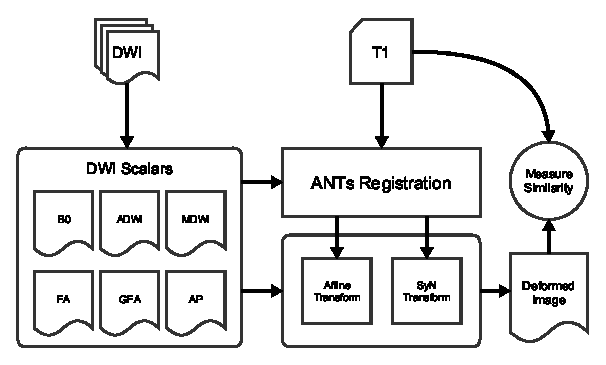
\includegraphics[width=0.8\linewidth]{figure1}
\end{tabular}
\caption{Illustrated overview of the processing steps to measure DWI to T1 registration similarities.}
\label{fig:APfigure1}
\end{figure}

\begin{figure}[ht]
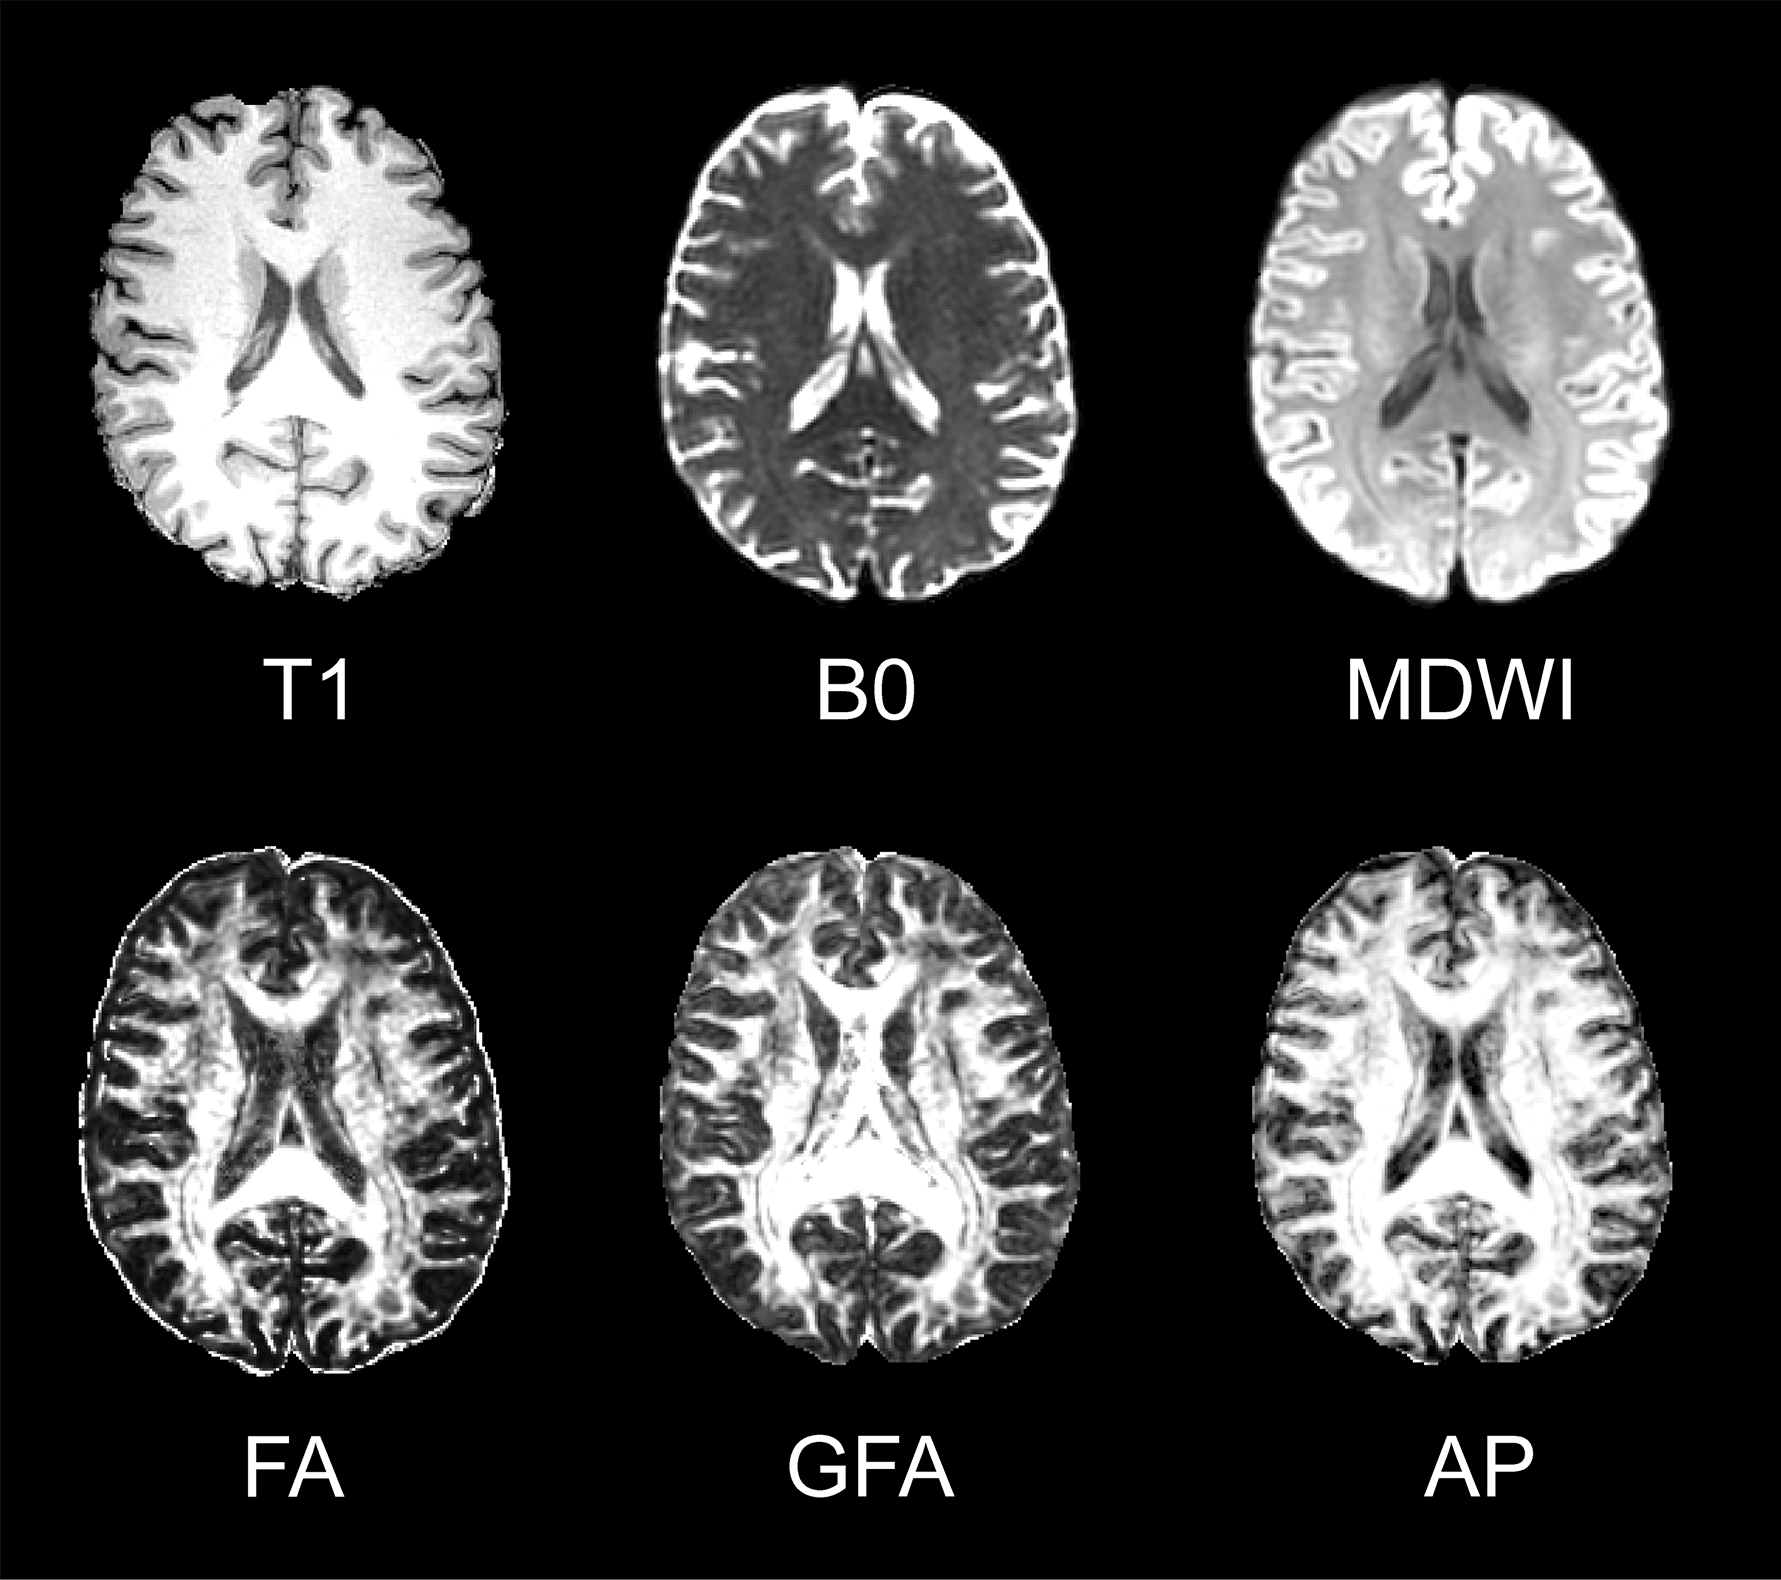
\includegraphics[width=\linewidth]{figure2}
\caption{DWI derived scalar images (B0, MDWI, FA, GFA, and AP) comparing to T1 (top left).}
\centering
\label{fig:APfigure2}
\end{figure}

\subsection{T1 to DWI Co-registration}
Registrations were performed using Anatomical Normalization Tools (ANTs) \cite{Avants2008b} with affine and symmetric diffeomorphic registration. MI was used as the cost function for affine registration, while CC and MI were used separately as the SyN registration cost-functions. Parameters for affine registration: step size = 0.1, metric = mutual-information (MI), convergence = 10000x10000x10000x10000x10000, shrink factors = 5x4x3x2x1, smoothing sigmas = 4x3x2x1x0mm. Parameters for symmetric diffeomorphic registration (SyN): MI metric weight = 1, MI bins = 32; CC metric weight = 1, CC radius = 3; convergence = 50x35x15,1e-7, shrink-factors = 3x2x1, smoothing sigmas = 2x1x0mm, and use-histogram-matching = true.

The resulting registration transforms from each DWI derived scalar image were applied to all DWI derived scalar image types including themselves using 3rd order B-spline interpolation, where they were projected into T$_1$ space. For each DWI scalar image, an identity transformation ($T_{\text{Identity}}$), affine-only transform ($T_{\text{Affine}}$), and affine with SyN transforms ($T_{\text{Affine}}$+SyN) were applied separately. MI and CC similarity metrics between the transformed DWI scalar and T$_1$ images were obtained using ANTs. Percent change in both CC and MI similarity scores for each type of transformed images were calculated as:
\begin{equation}
\text{Percent Change} = \frac{\text{Transformed} - \text{Identity}}{\text{Identity}} \times 100
\end{equation}
The higher the percent change is, the more similar the transformed DWI scalar and T$_1$ images are after accounting for the identity transformation.
ANOVA and Tukey post-hoc tests were performed using R statistics software (R Core Team, 2014) to compare differences in percent changes between similarity scores of images deformed by their own $T_{\text{Affine}}$+SyN (autodeformation: $D_{\text{auto}}$; e.g. comparing pre- to post-FA scores when FA image was used as the intermediate) as well as similarity scores across groups ($D_{\text{all}}$; e.g. comparing scores resulting from using the FA intermediate to transform all other image types). 

Additionally, we used a joint log-histogram of all the DWI derived scalar images to examine possible group biases in DWI scalar types. We intuited that the scalar maps can roughly be divided into two primary groups: those that are directly computed from the DWI directions (DSG), and share similar intensity profiles, such as B0, MDWI, ADWI; and those computed from anisotropic diffusion models (ASG), such as FA, GFA, and AP. It’s possible that there exists a degree of orthogonality between image types, such that there may be no single image type that can equally translate the registration improvements to other images with different intensity profiles. The joint log-histogram is to check for the existence of this type of orthogonality. 

\subsection{Results}
Pair-wise joint log histogram (Figure \ref{fig:APfigure3}) of the DWI derived scalar images revealed distinct correlation patterns in some pairs of images. FA–AP and FA–GFA showed distinct diagonal correlations patterns with each other; while B0 showed no clear pattern of correlation with other image types, with the exception of MDWI. The scalar images FA, GFA and AP are parameter maps derived from diffusion models, whereas B0 and MDWI are directly derived from the DWI image sequence. We thus grouped FA, AP, and GFA based on their intensity histogram correlations as the anisotropic scalar group (ASG), while B0 and MDWI form a directly derived scalar group (DSG). 

\begin{figure}[p]
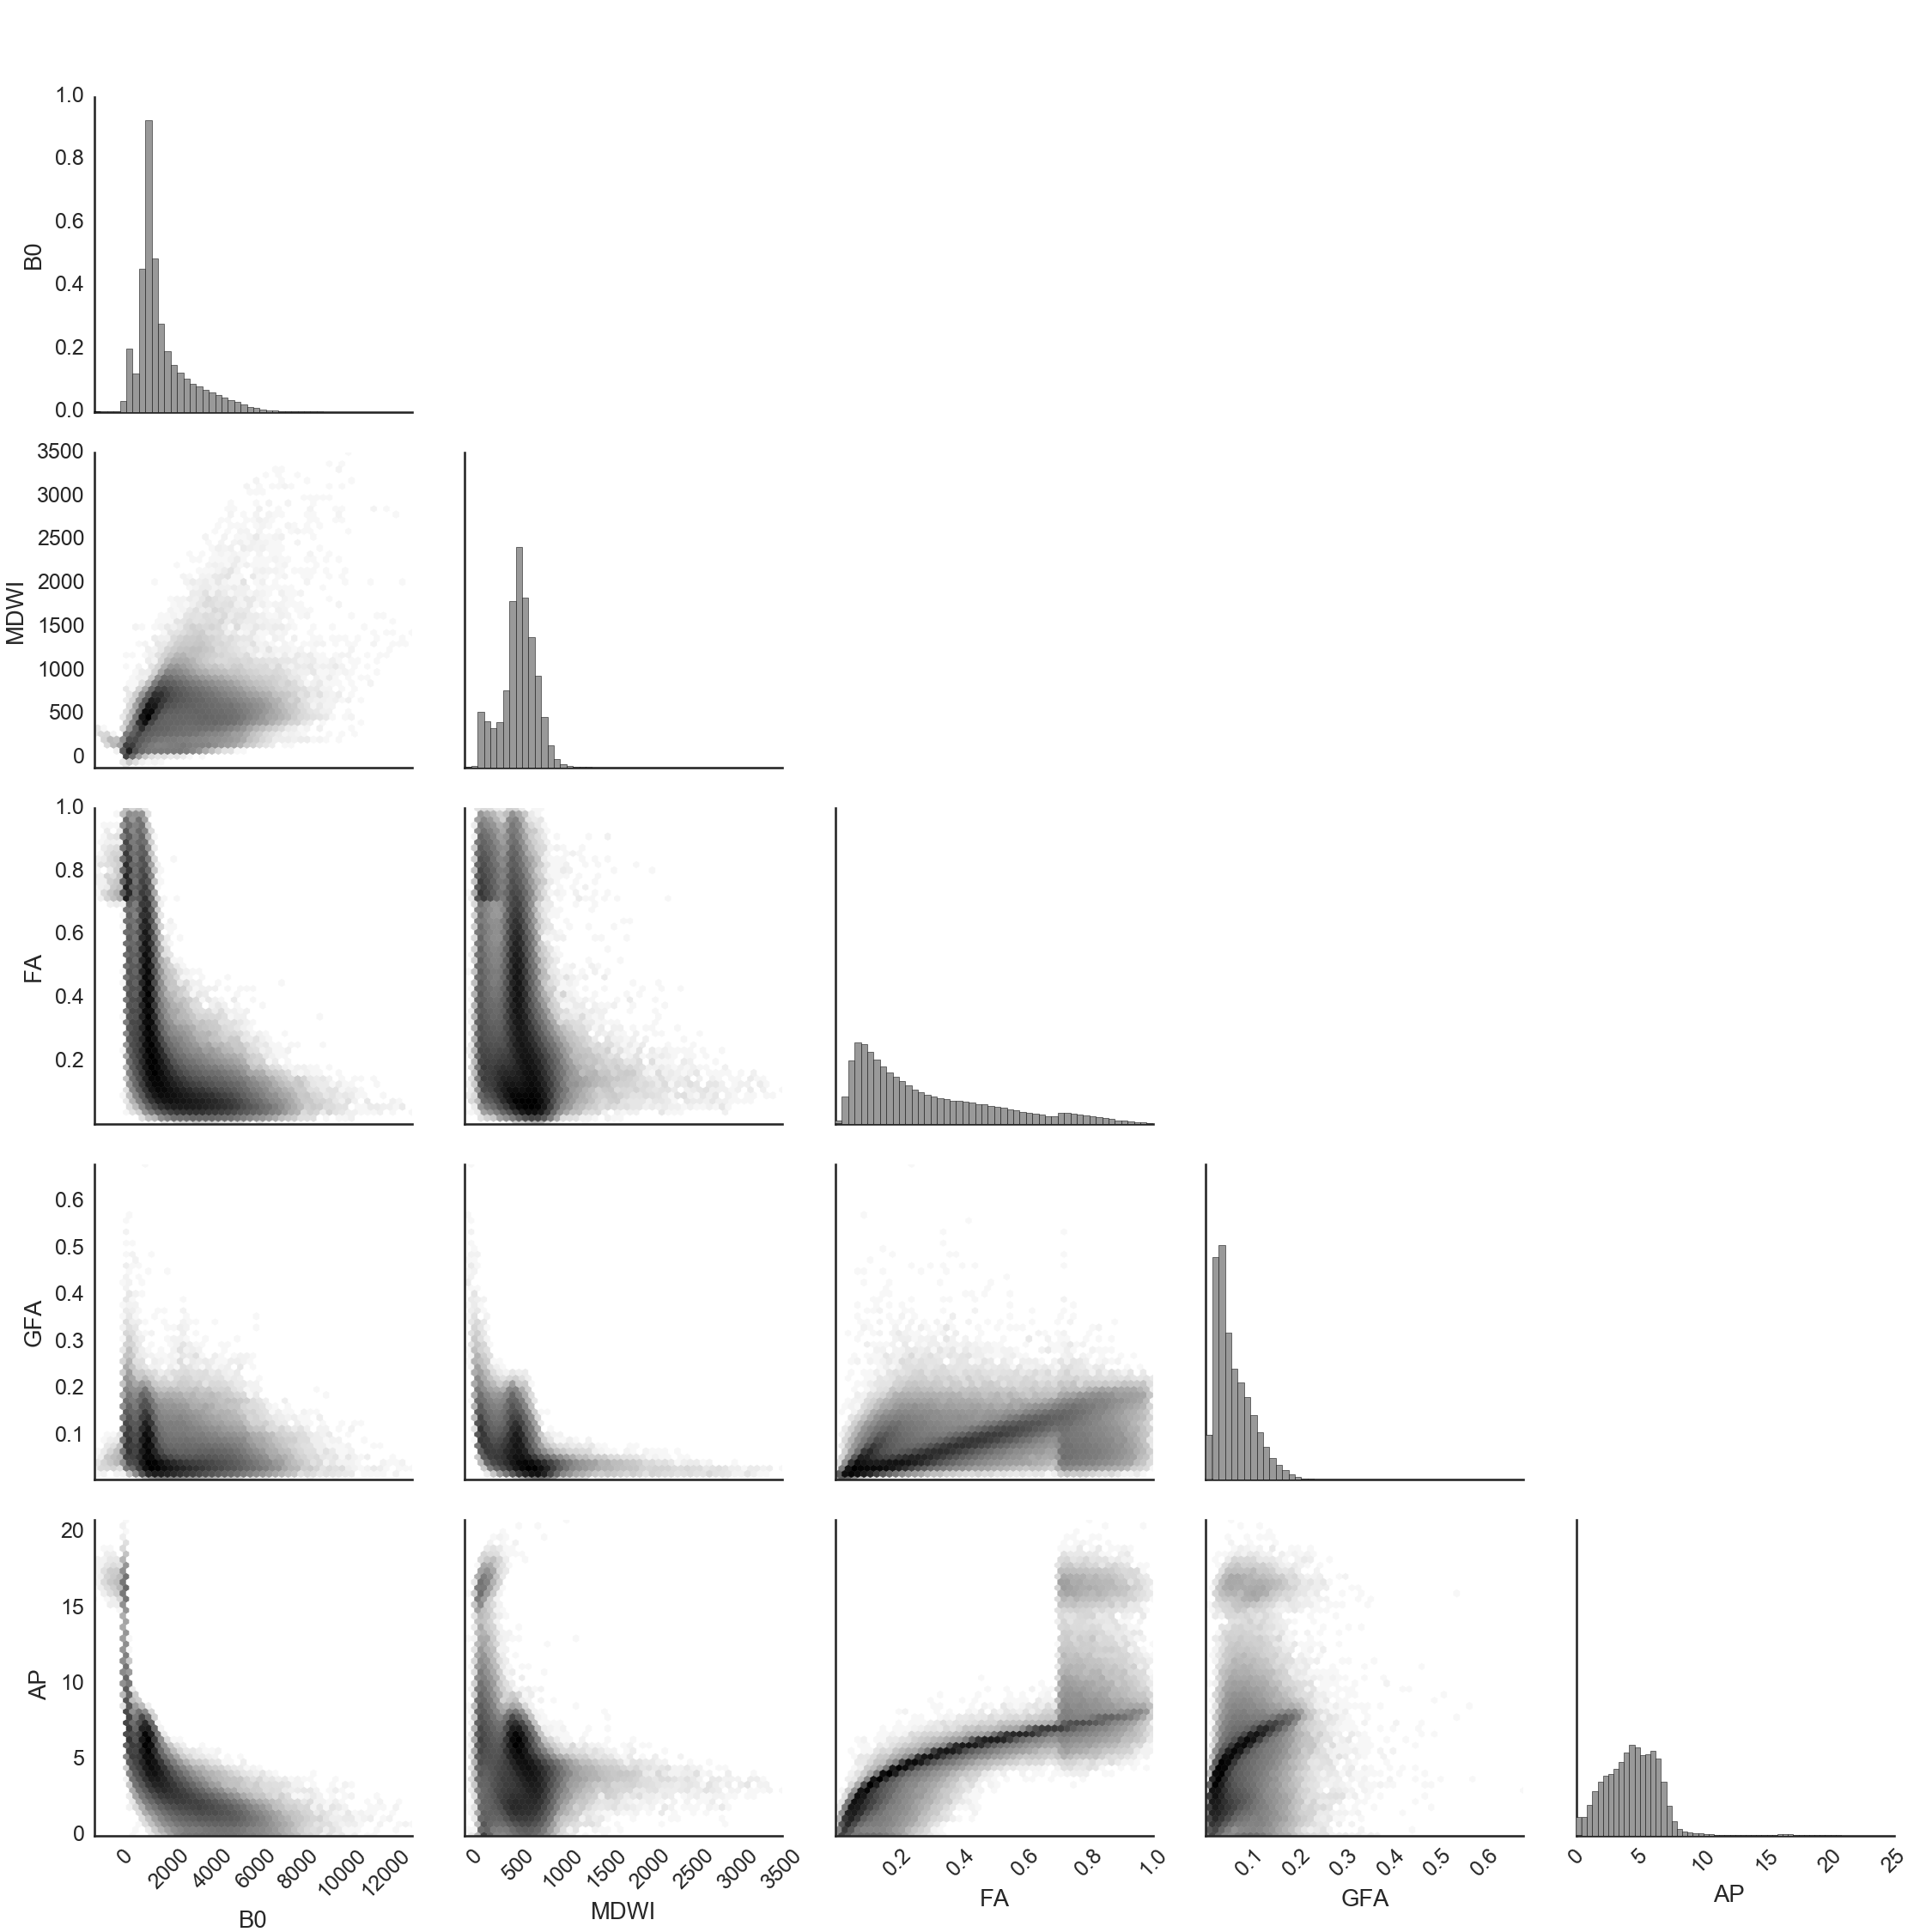
\includegraphics[width=\linewidth]{figure3}
\caption{Pair-wise joint log histogram of the DWI derived scalar images.}
\centering
\label{fig:APfigure3}
\end{figure}

\begin{figure}[p]
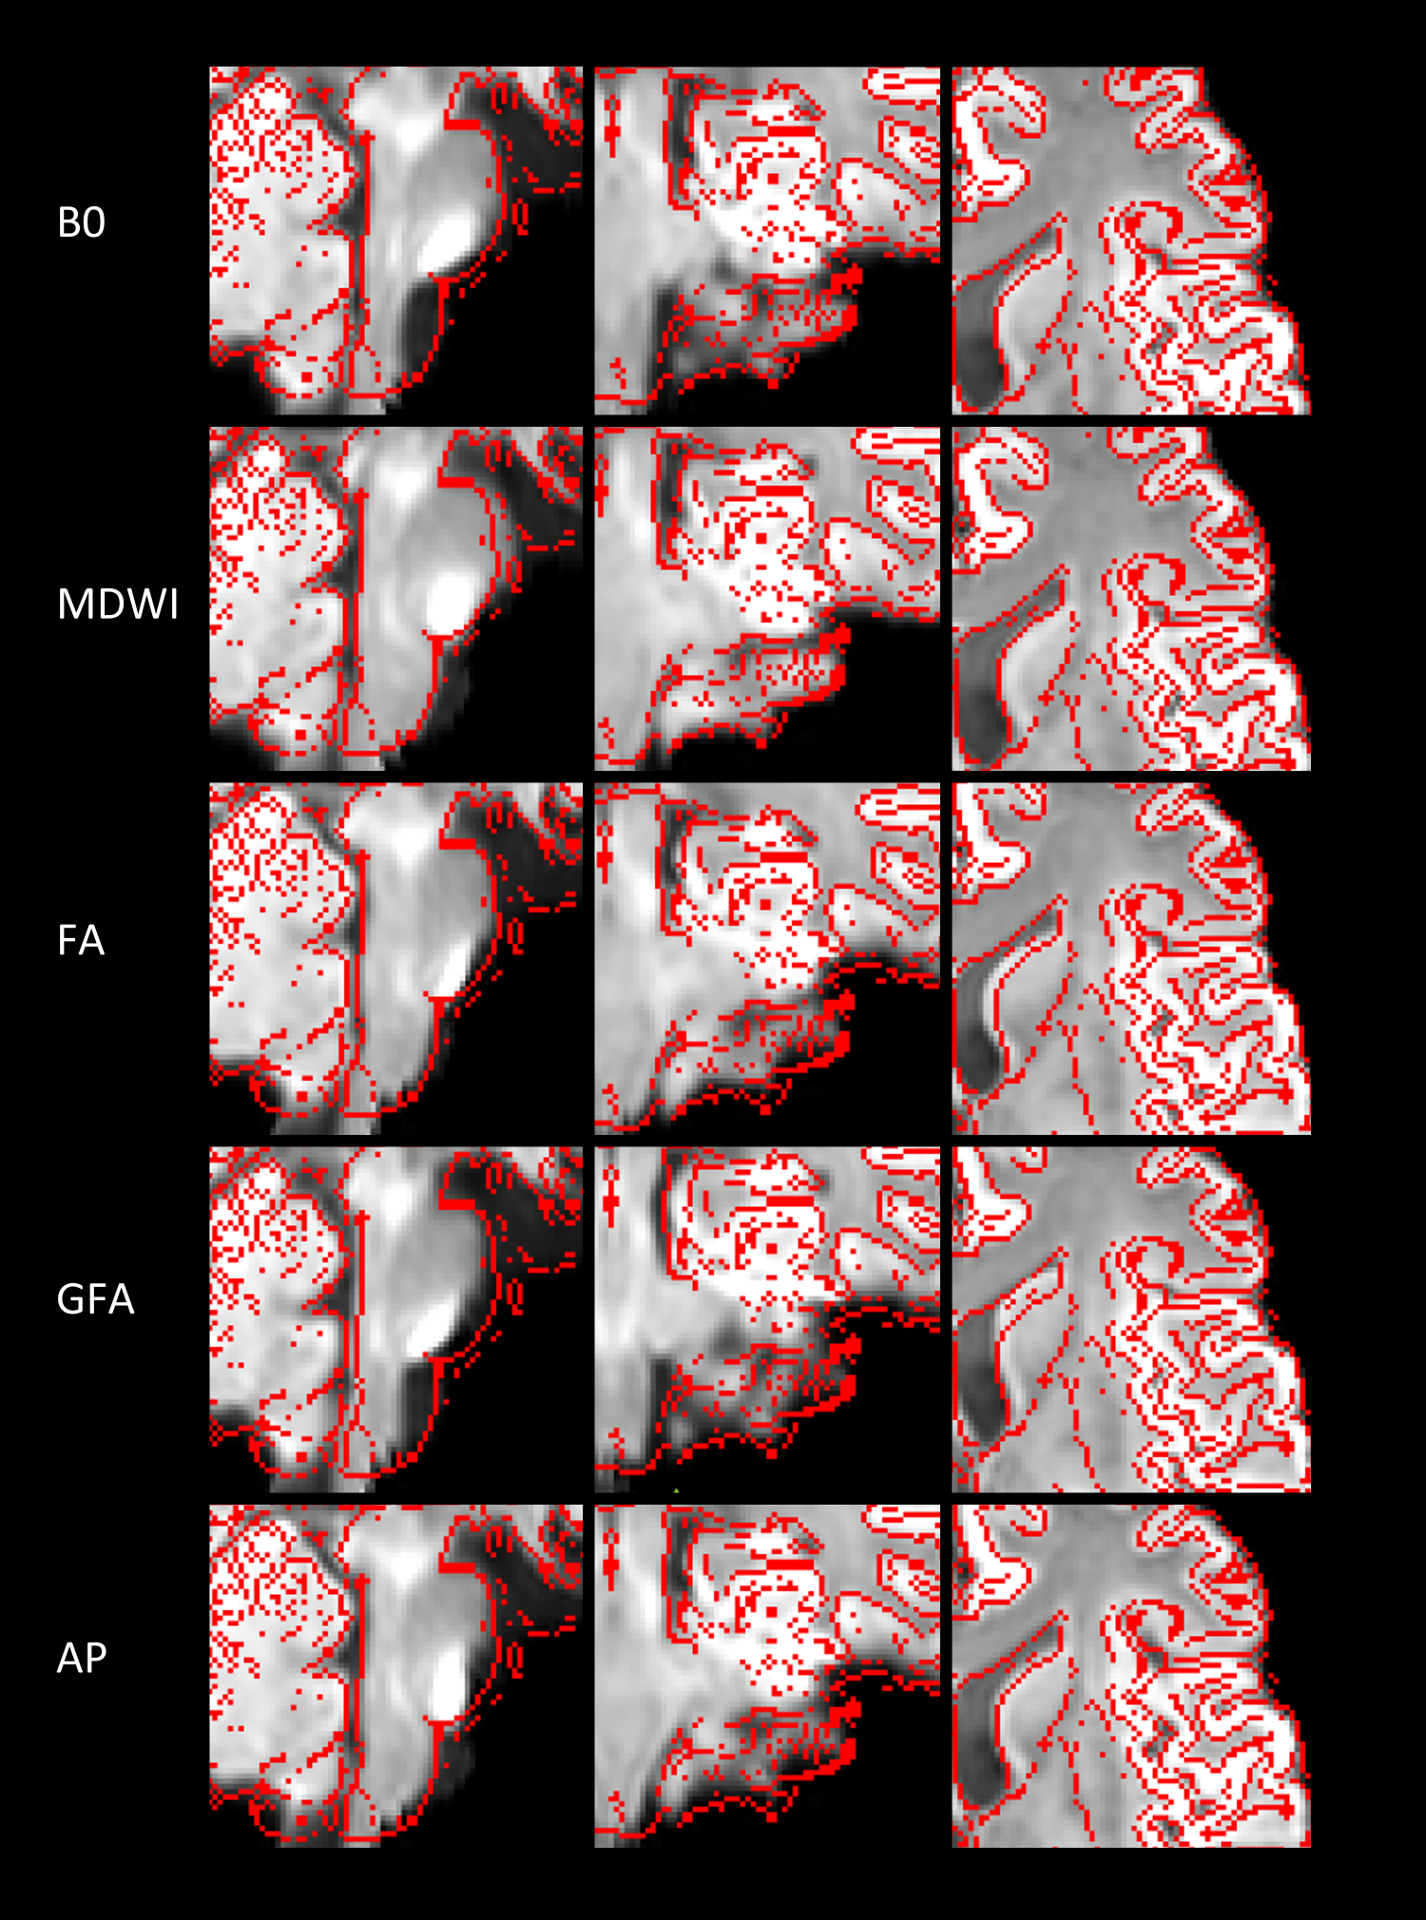
\includegraphics[width=\linewidth]{figure4}
\caption[Visual comparisons of MDWI to T1 co-registrations.]{Visual comparisons of MDWI to T1 co-registrations. 
Shown are examples of MDWI images from one subject deformed using different registration transforms derived from the different image intermediates. 
T1 is overlaid as thresholded outlines in red. 
Primary differences in registration quality can be found in the brainstem (left and middle columns), and in the lateral ventricles, especially in the ventricular-caudate boundary (right column). }
\centering
\label{fig:APfigure4}
\end{figure}

\subsubsection{Differences in initial similarity scores affect registration accuracy}
Visual overlay of MDWI to T1 co-registrations (Figure \ref{fig:APfigure4}) suggests that DWI derived scalar image with higher initial CC and MI scores (Figures \ref{fig:APfigure5}) appear to result in more accurate registrations in the brainstem, insula, temporal cortices, and lateral ventricles (especially around the ventricular-caudate boundary where CSF/grey/white-matter are found in close proximity) compared to the other image types. Visually, B0, FA and GFA show registration inaccuracies fitting the areas surrounding the brainstem and the lateral ventricles (Figure \ref{fig:APfigure4}), while MDWI and AP result in improved registration in these key areas. The results of MDWI and AP are visually very similar.

The initial T1–intermediate CC and MI similarity scores without any applied transformation ($T_{\text{Identity}}$) showed varied initial values. MDWI showed the highest initial CC scores, with FA images showing lowest initial CC (Figure \ref{fig:APfigure5}); AP showed similar initial CC score with B0 and GFA. For MI scores (it is important to note that a more negative MI score implies higher similarity in this study), AP showed very similar initial MI score when compared to MDWI (best), while GFA resulted in the highest (worst) initial MI score.

\subsubsection{Registration improvements are not uniformly transferred when applied to other image types}
The progression of similarity scores following $T_{\text{Affine}}$ and $T_{\text{Affine}}$+SyN for each of the scalar images (B0, ADWI, MDWI, FA, GFA, and AP) showed similar trends between CC and MI cost-functions (Figures \ref{fig:APfigure5},  Figure \ref{fig:APSup1}; top rows). In general, the similarities of the images between T1 and transformed DWI scalar images increased marginally after $T_{\text{Affine}}$, and substantially after $T_{\text{Affine}}$+SyN for most of the co-registration transforms. An exception is FA transforms, where CC scores decreased when the transform was applied to other images (Figure \ref{fig:APfigure5}; rows 1-2, column 4), with the exception of AP. 

Improvement in CC and MI measures were not uniform for all DWI derived scalar images; this was better illustrated by percent changes (Figures \ref{fig:APfigure5}; bottom rows). Different intermediate transforms differentially affected the scores in accordance with the degree of intensity correlations as measured in Figure \ref{fig:APfigure3}. Therefore, DSG transforms preferentially improved DSG, and ASG transforms improved ASG images. FA transforms, however, are notable, where CC scores across all DWI derived scalar images diverged for both CC and MI cost functions (Figures \ref{fig:APfigure5}, Figure \ref{fig:APSup2}; column 4). In fact, FA transforms substantially decreased DSG CC scores, and also negatively impacted DSG MI scores as well. FA transforms also showed exception to GFA, where it affected GFA negatively similar to DSG images. GFA behaved more like DSG images, where B0 and MDWI all favorably affected its CC and MI scores, while at the same time it was strongly affected by AP as well. However GFA seem to behave differently under autodeformation, as evident by its distinct MI changes (Figures \ref{fig:APfigure5}; column 5). AP transforms showed the least amount of variability when applied to DWI derived scalar images, and consistently improved all the image scores. 

\subsubsection{AP-derived transforms show the most consistent improvements when applied to other image types}

Between-group statistical comparisons of only $T_{\text{Affine}}$+SyN percent change revealed significant findings. Under the CC cost-function (Figure \ref{fig:APfigure6}), percent change in $D_{\text{auto}}$ (Figure \ref{fig:APfigure6}, bottom panel, column 3) showed that FA and GFA have the highest percent change, while AP has the lowest percent change. With MI scores, $D_{\text{auto}}$ showed that only GFA percent changes are significantly greater than others (Figure \ref{fig:APfigure6}, bottom panel, column 4). GFA, however, also shows the greatest variability in distribution (Figure \ref{fig:APfigure6}, top panel, column 4).  $D_{\text{all}}$ in contrast, showed that FA is an outlier where its percentage change is significantly lower than all other images; it is also notable that it shows a distinct bimodal distribution (Figure \ref{fig:APfigure6}, top panel, column 1); GFA was shown to be significantly higher than B0, MDWI and FA, but not AP. MI percent changes are not significantly different from each other (Figure \ref{fig:APfigure6}, bottom panel, column 2). MI cost-function results were similar to that of the CC cost-function (Figure \ref{fig:APSup2}). 

\section{Discussion}

This study presents a comparison of the DWI derived scalar image to use for T1 to DWI co-registration. AP images showed the most consistent improvements in image scores across all of the intermediate scalar images tested, suggesting that AP can offer the most consistent T1-DWI co-registration improvements, while FA and GFA images are poorer choices. We observed, via CC and MI scores, that non-linear registration shows similar trends in registration performance. DWI derived image registration improvements show biases that depend on the intensity correlations with directly derived scalar image group (DSG) or anisotropic scalar image group (ASG) similarities. FA showed significantly lower MI and CC similarity scores that worsened registration results. GFA showed a significant increase in similarity scores, but also greater variability in percent increases when its transform was applied to other image types – suggesting that while this measure is better than FA alone, it is still highly unreliable across subjects. 

\subsubsection{Registration improvements are biased towards similar image intensity groups}

The log joint histogram showed that there is a degree of intensity orthogonality between FA, AP, and GFA as a group (ASG) compared to B0, ADWI and MDWI (DSG), suggesting that there is some connection between co-registration performance and intensity similarity (Figure \ref{fig:APfigure3}). The greater the intensity similarities between the two images, the greater the effect of the same set of registration transforms. Intensity similarity is not the only factor, however, as evident by the exception to this rule in FA and GFA deformation results (Figure \ref{fig:APfigure5}). This suggests that intensity orthogonality is not a limiting factor in registration transfer across these scalar images. Therefore, our hypothesis that there exists a better DWI intermediate scalar image that can improve multimodal registration is correct.

\subsubsection{Autodeformation is not sufficient to assess registration intermediate performance}

Our study demonstrates clear differences in initial similarity scores (i.e. CC and MI) across different DWI scalar images when compared to T1, where MDWI had the highest initial CC and MI scores.  Moreover, the AP and MDWI images clearly outperformed the B0, FA, GFA and intermediates in visual inspections.

As expected, autodeformation (e.g. FA to T1 registration applied to the FA image, from greek autos: self) yielded the best metric of similarity compared to when the transform was applied to other image types. The optimal T1-DWI co-registration performance of an intermediate image could be identified by the image’s deformation by its own transform. However, we show that only comparing the autodeformation results is not ideal (Figure \ref{fig:APSup1}, \ref{fig:APSup2}). Specifically, while the FA autodeformation (using $T_{\text{Affine}}$+SyN) performed better compared to all other autodeformations, registrations of other scalar images based on FA transformations clearly resulted in the worst results. Therefore, future comparisons of candidate intermediate images should consider not only the autodeformation, but also the ability of a transform to deform other scalar images. It is also worth noting that affine transformations marginally improve MI scores – which is expected as the head orientations within MR scanners usually do not deviate very far between acquisitions, but most registration improvements stem from corrections to DWI distortions through non-linear registration.

The larger percent change improvements in FA and GFA can be explained by the ceiling effect of registration, where images that are initially more similar to the T1 anatomical image (e.g. MDWI or AP) would have less room for improvements compared to those that are less similar (e.g. FA or GFA). As such, the absolute difference in similarity scores should still be included in the final assessment of registration. It is also important to note that computational algorithms using CC and MI as the optimization metric in the registration process itself cannot fully characterize the goodness-of-fit of one set of images when matched with another. Therefore, our current use of these scores does not preclude the possibility that certain image sub-regions would be better registered using other scalar image types under specific conditions. Moreover, the method of estimating an undistorted DWI with reversed phase-encoding images may still be superior to the use of image intermediates, described here, when this approach is possible. Nonetheless, the post-processing use of intermediate images combined with reverse-phase corrected DWI may result in improved registrations.

As a new DWI derived scalar image, our study is the first to evaluate AP for the purpose of T1-DWI co-registration. AP images can consistently improve similarity outcomes for the various image types and shows more consistent similarity outcomes when compared to other modalities. Further research is needed to determine the optimum method for AP normalization. 

\subsubsection{Limitations}

One important limitation is that the DWI voxel sizes are not isotropic. For this study, the DWI images were acquired at 0.94x0.94x3 $mm^3$ voxel resolution. The dataset was acquired on a 3T GE HDx MRI with 8-channels head coil, and therefore does not permit DWI scans of less than 2.6 mm isovoxel resolution at a clinically acceptable scanning time. As such, we compromised on an anisotropic voxel resolution to gain in-plane resolution. Although recent authors have suggested using isotropic up-sampling of MR images to improve image quality \cite{Dyrby2014}, we decided not to introduce up-sampling into our processing pipeline in order to avoid the possibility of additional interpolation-introduced artifacts that may bias towards certain image types.  Clinical datasets are often acquired under time and resource constraints, and therefore we believe our findings will be novel for the application of clinical T1-DWI co-registrations at less than ideal conditions.

\section{Conclusions}
This study demonstrated that for T1-DWI co-registration, using AP as the DWI derived scalar image type resulted in improved registration performance. AP offers more consistent registration across DWI derived scalar images. AP requires the calculations of spherical harmonic coefficients as a preprocessing step, and therefore stabilizes when there are greater than 28 gradient directions. It is thereby unsuitable for some legacy DWI datasets acquired with fewer than 28 directions. MDWI can be readily obtained from existing DWI sequences, and is therefore suitable for all existing datasets. We generally recommend the use of AP where available. In the case where calculation of AP images is not possible, MDWI is a viable alternatives as T1-DWI co-registration intermediates. FA and GFA were the poorest performers, and we recommend not using them for registration purposes.

\afterpage{

    \begin{figure}[p]
    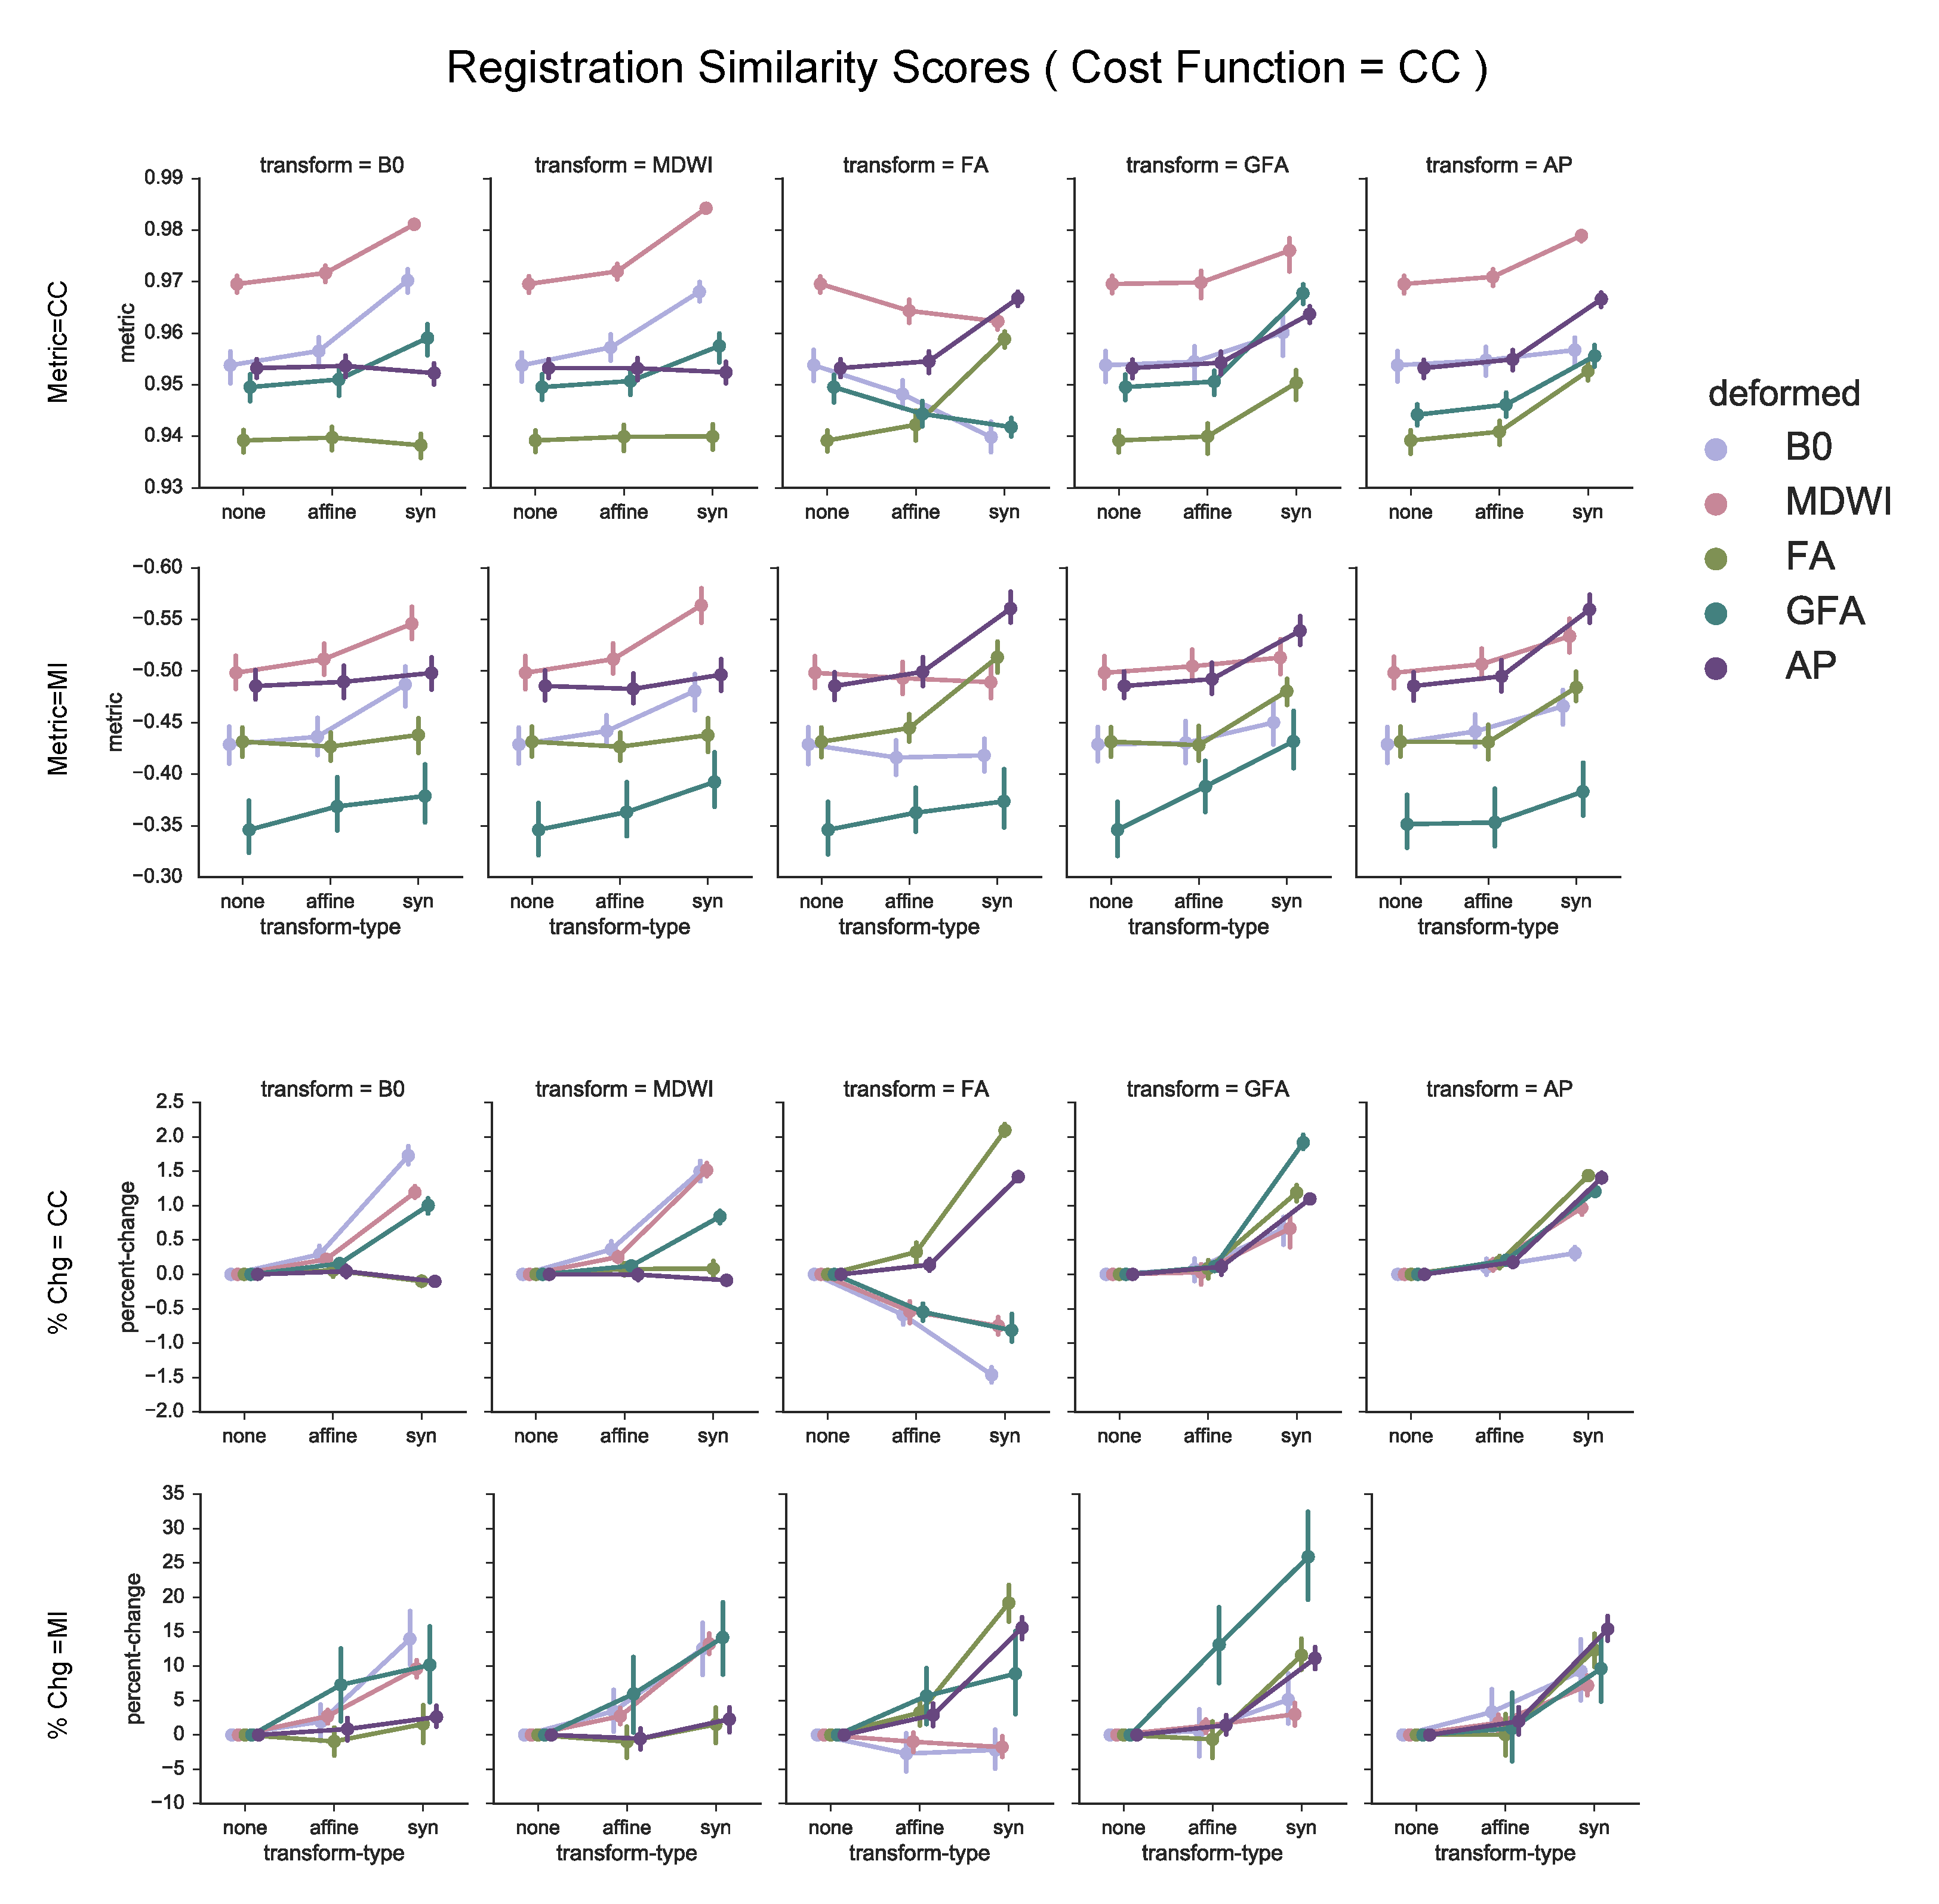
\includegraphics[width=\linewidth]{figure5}
    \caption[Similarity scores between deformed dMRI scalar images and T1 following registrations with CC as cost function for SyN.]{Similarity scores between deformed dMRI scalar images and T1 following registrations with CC as cost function for SyN. 
    Three steps of the registration process are plotted: Initial identity transformation (none), affine transformation (affine) and affine+SyN transformation (SyN).
    Top panel shows similarity scores as measured by CC and MI, and bottom panel shows average percent change progressions of CC and MI across dMRI scalar images from \protect $T_{\text{Affine}}$ to \protect $T_{\text{Identity}}$, and from \protect $T_{\text{Affine}}$+SyN to \protect $T_{\text{Affine}}$. The error bars denote standard deviation across subjects.}
    \centering
    \label{fig:APfigure5}
    \end{figure}


    \clearpage
    
    \thispagestyle{empty}% empty page style (?)
    \begin{landscape}% Landscape page
    
        \begin{figure}[p]
        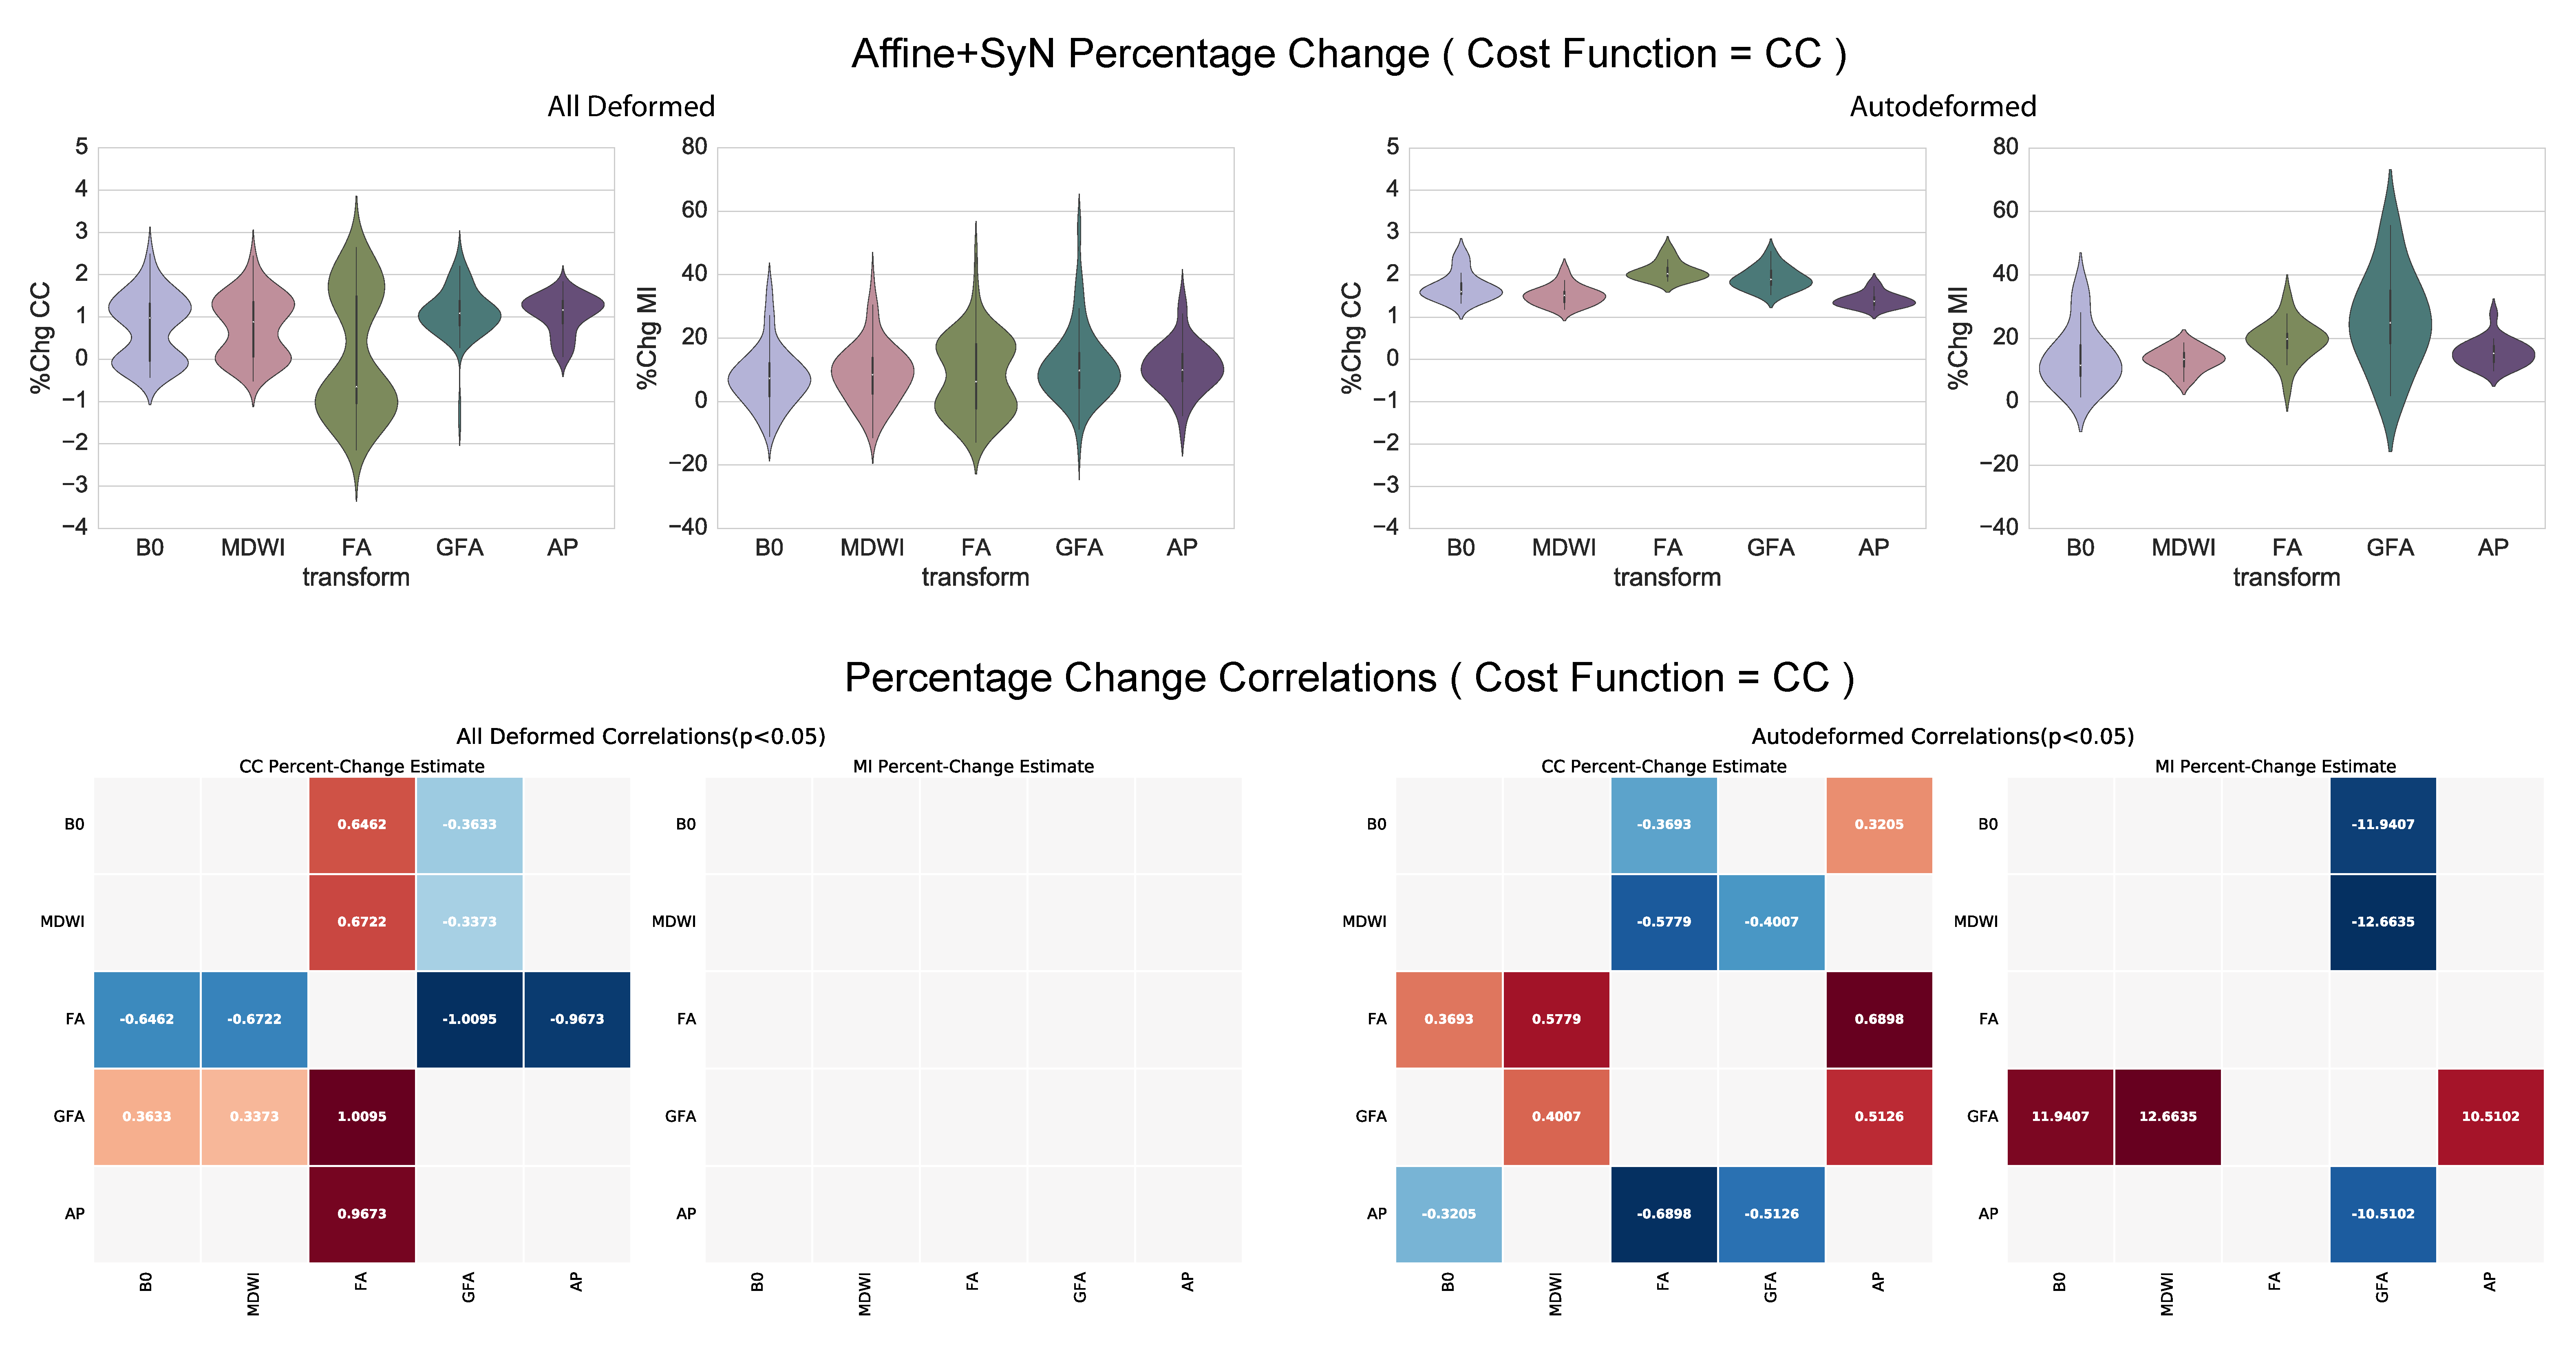
\includegraphics[width=\linewidth]{figure6}
        \caption[Percent changes of similarity score from \protect $T_{\text{Affine}}$+SyN to \protect $T_{\text{Identity}}$ with CC as cost function.]{
        Percent changes of similarity score from \protect $T_{\text{Affine}}$+SyN to \protect $T_{\text{Identity}}$ with CC as cost function. Top row shows the violin plot distribution of CC and MI percent change under All Deformations and Autodeformations. Bottom row plots the statistically significant pair-wise correlations of the different transforms. 
        Under All Deformations (\protect $D_{\text{all}}$), CC percent change of FA is shown to be significantly lower (p<0.05) than that of all other transform types. GFA can be observed to have higher percent change than that of B0, MDWI, and FA. Under Autodeformations (\protect $D_{\text{auto}}$), CC percent change of FA and GFA are significantly higher than others, while AP has lower percent change. MI shows little percentage between all the images; GFA shows significantly differences under \protect $D_{\text{auto}}$, but also shows high variability.}
        \centering
        \label{fig:APfigure6}
        \end{figure}
    \end{landscape}
    
    \clearpage


    \begin{figure}[p]
    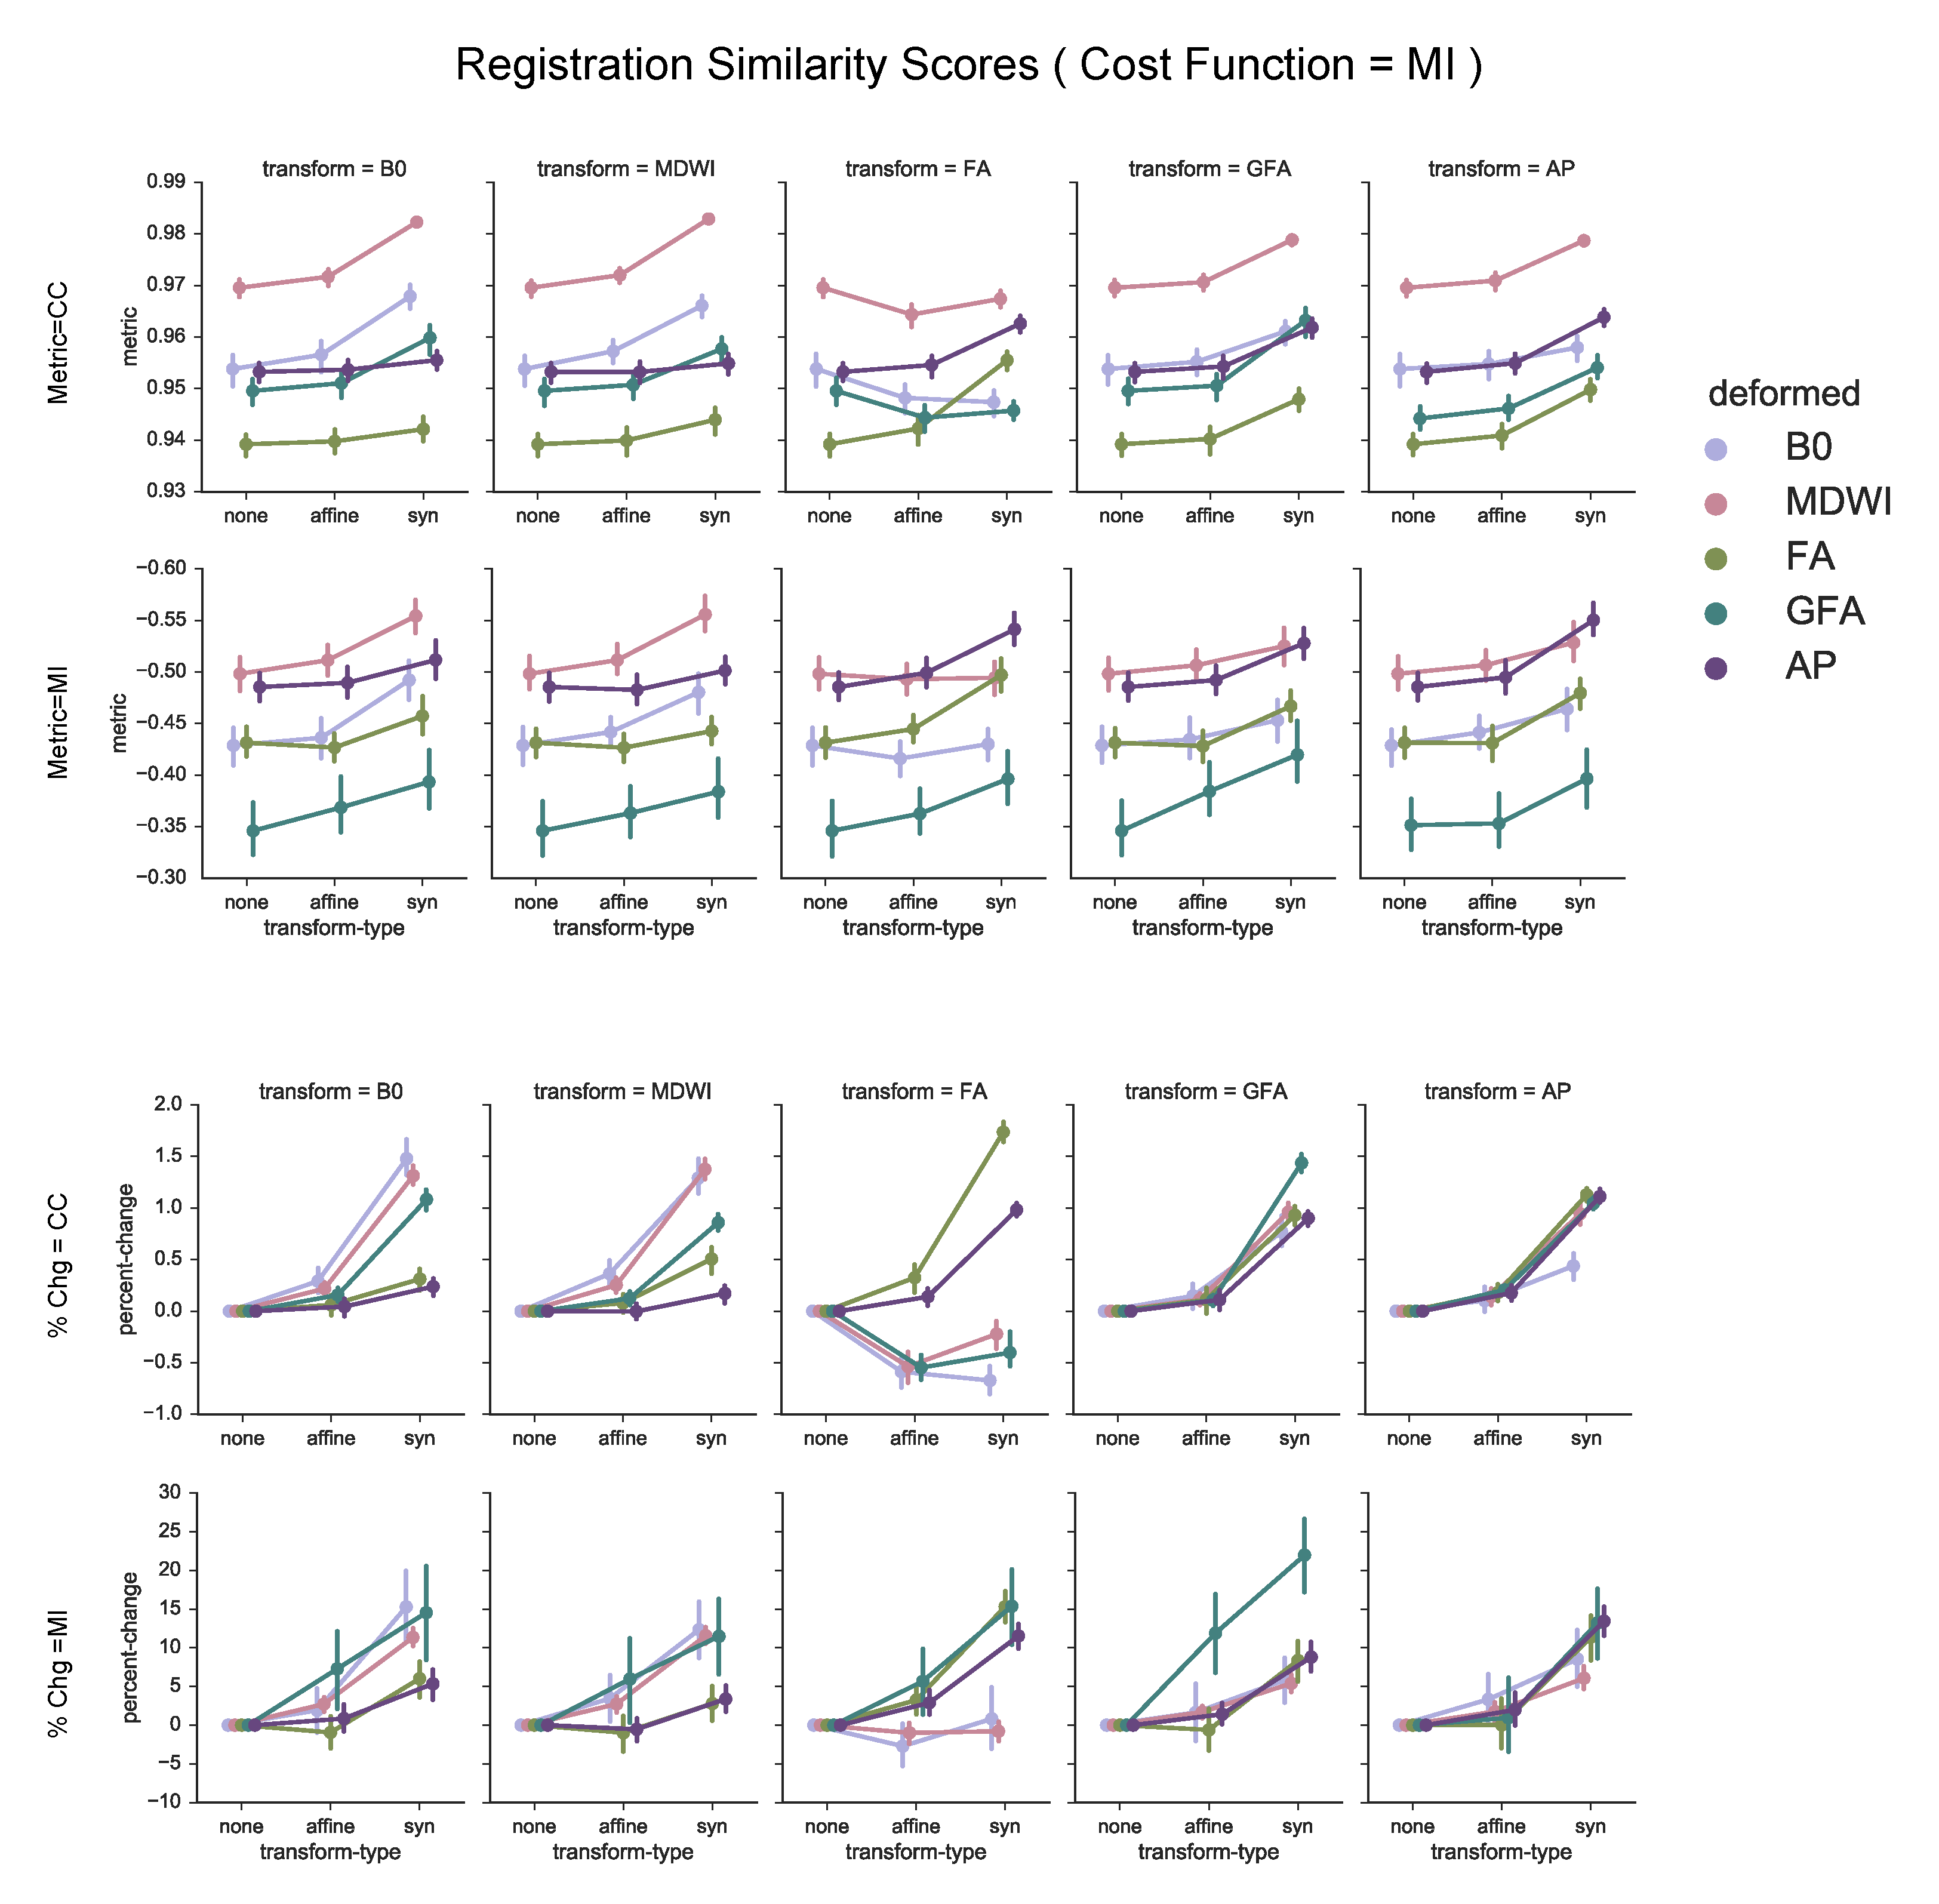
\includegraphics[width=\linewidth]{sup1}
    \caption[Similarity scores between deformed dMRI scalar images and T1 following registrations with MI as cost function for SyN. ]{Similarity scores between deformed dMRI scalar images and T1 following registrations with MI as cost function for SyN. 
    Three steps of the registration process are plotted: Initial identity transformation (none), affine transformation (affine) and affine+SyN transformation (SyN).
    Top panel shows similarity scores as measured by CC and MI, and bottom panel shows average percent change progressions of CC and MI across dMRI scalar images from \protect $T_{\text{Affine}}$ to \protect $T_{\text{Identity}}$, and from \protect $T_{\text{Affine}}$+SyN to\protect  $T_{\text{Affine}}$.}
    \centering
    \label{fig:APSup1}
    \end{figure}

    \clearpage
    
    \thispagestyle{empty}% empty page style (?)
    \begin{landscape}% Landscape page
        \begin{figure}[p]
        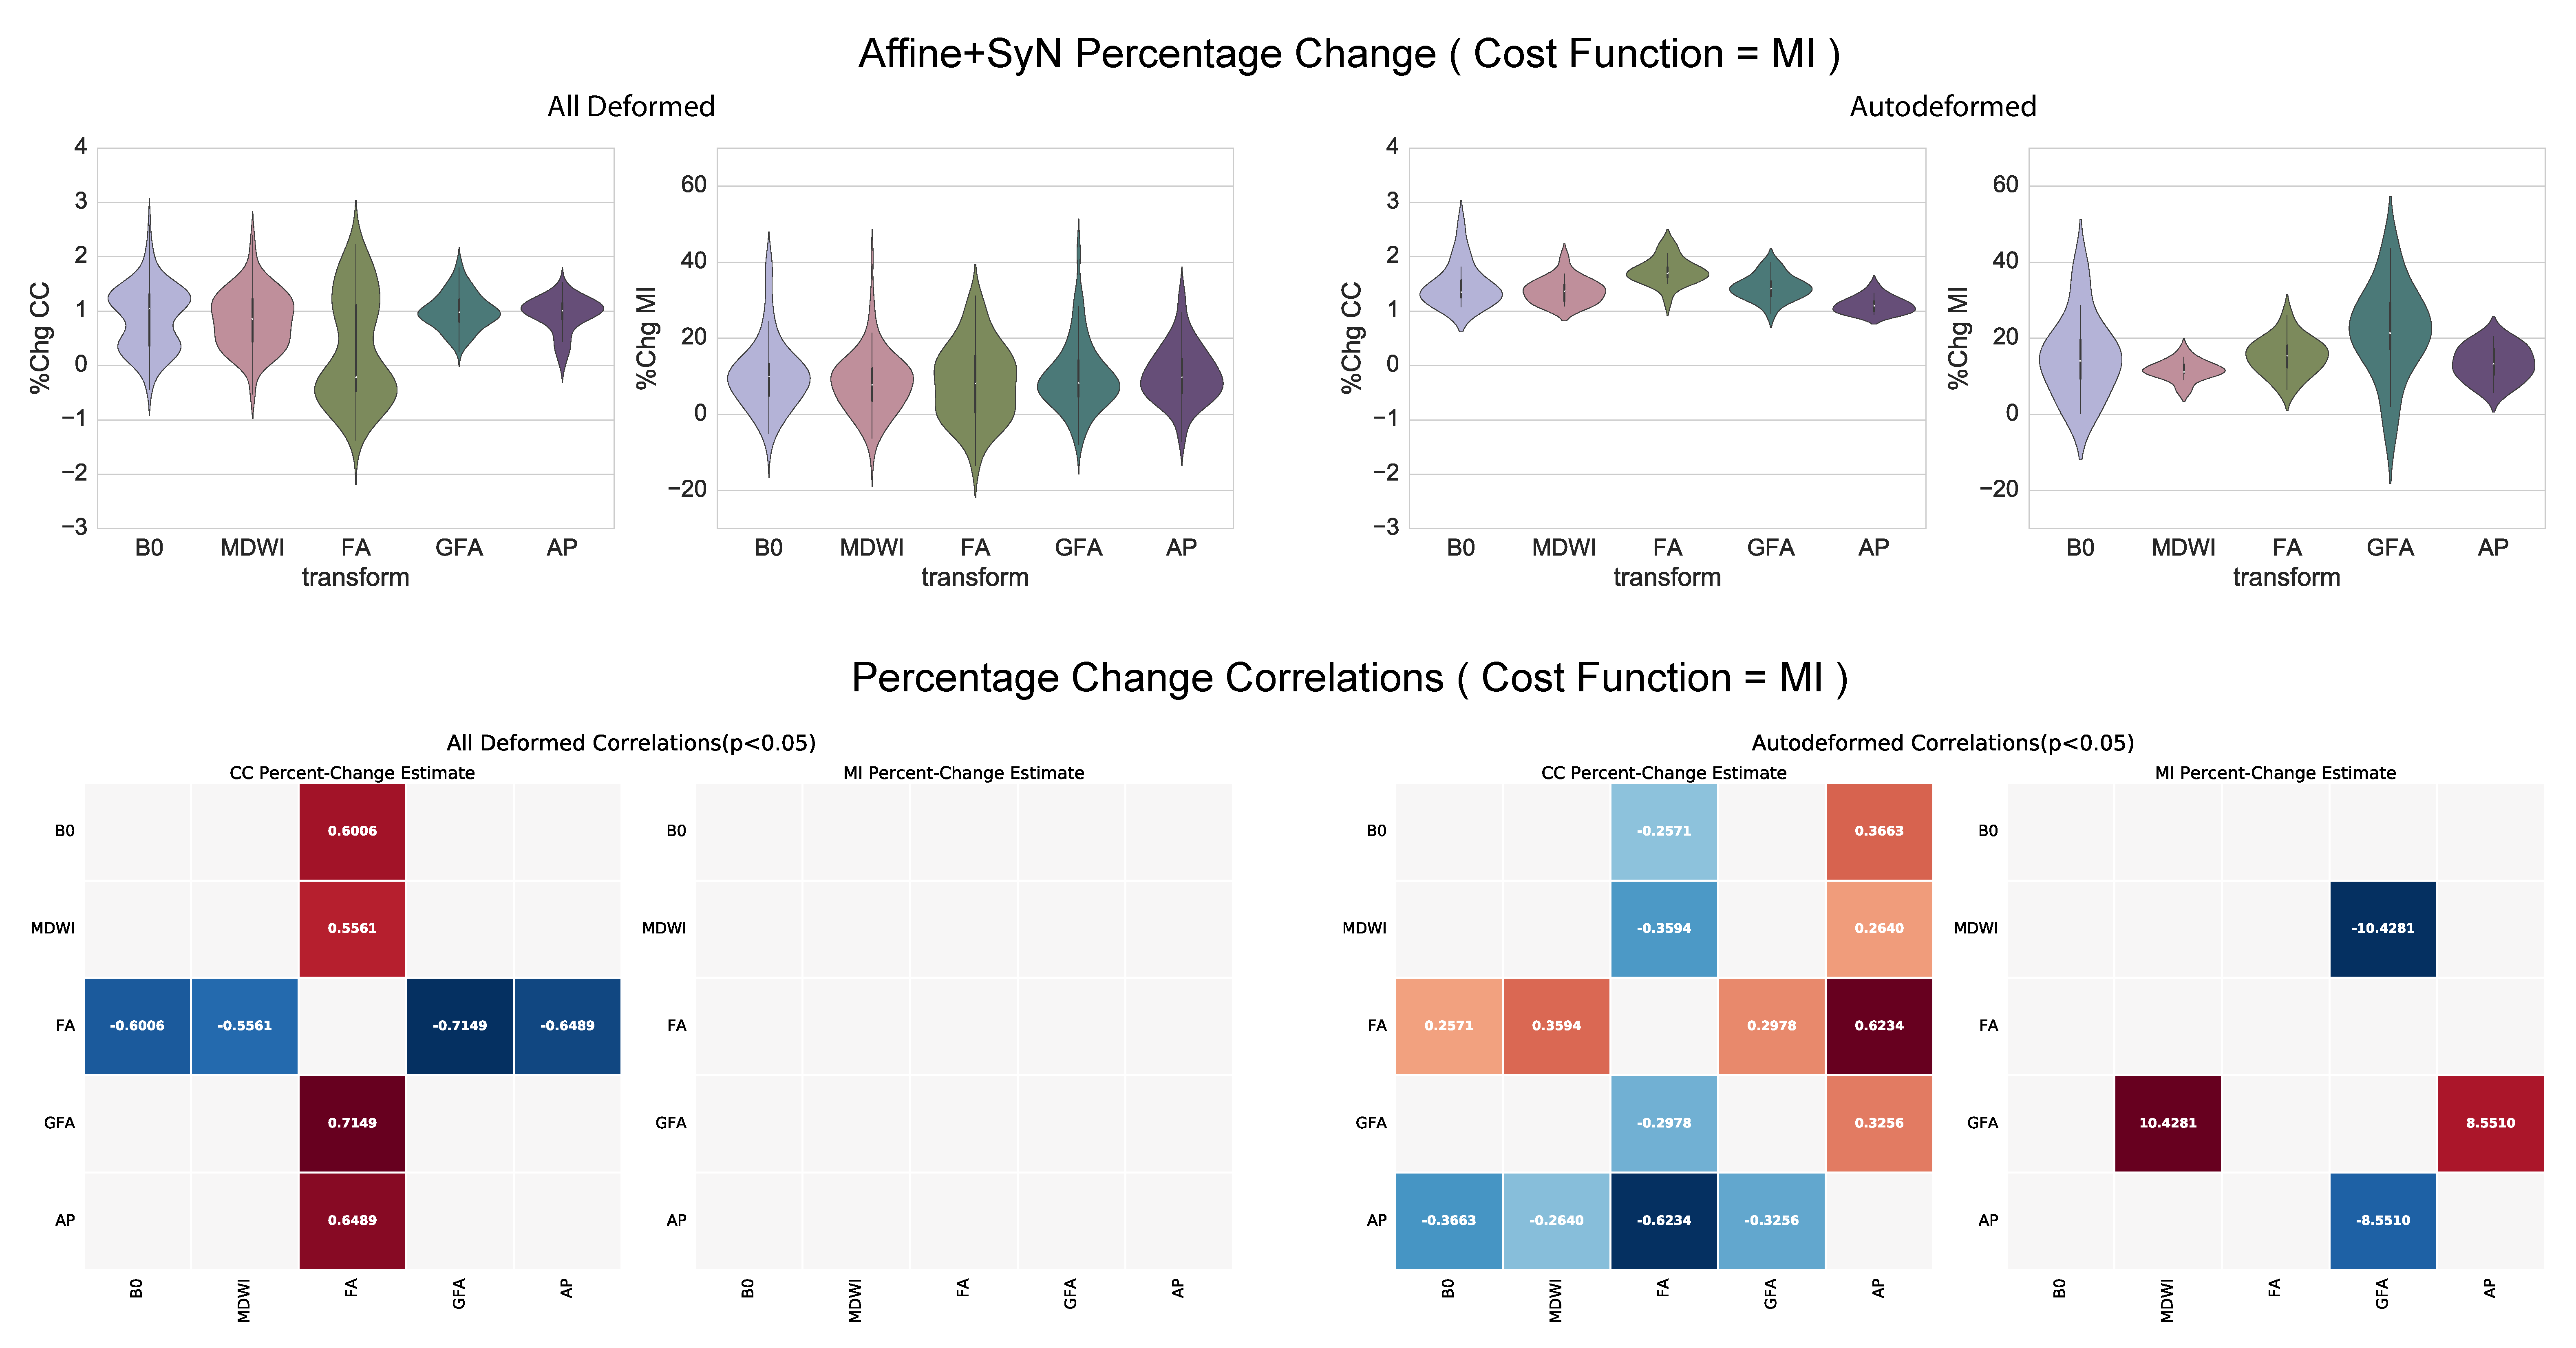
\includegraphics[width=\linewidth]{sup2}
        \caption[Percent changes of similarity score from \protect $T_{\text{Affine}}$+SyN to \protect $T_{\text{Identity}}$ with MI as cost function.]{Percent changes of similarity score from \protect $T_{\text{Affine}}$+SyN to \protect $T_{\text{Identity}}$ with MI as cost function. Top row shows the violin plot distribution of CC and MI percent change under All Deformations and Autodeformations. Bottom row plots the statistically significant pair-wise correlations of the different transforms.
        Under all deformations ( \protect$D_{\text{all}}$), CC percent change of FA is shown to be significantly lower (p<0.05) from that of other transform types. In autodeformations (\protect$D_{\text{auto}}$). FA has higher percent change. MI percent changes show little differences, and once again highlights the high variability of GFA. }
        \centering
        \label{fig:APSup2}
        \end{figure}
    \end{landscape}
}
\graphicspath{{images/sagit/}}

\chapter{STUDY III: Merged Group Tractography Evaluation with Selective Automated Group Integrated Tractography}
\chaptermark{Study III}
\label{section:study3}

This study was published in Frontiers In Neuroanatomy \textcopyright 2016:

\bibentry{Chen2016}

\section{Abstract }
\textbf{Introduction:} Tractography analysis in group-based studies across large populations has been difficult to implement. We propose Selective Automated Group Integrated Tractography (SAGIT), an automated group tractography software platform that incorporates multiple dMRI practices which will allow great accessibility to group-wise dMRI. We use a merged tractography approach that permits evaluation of tractography datasets at the group level.  We also introduce an image normalized overlapping score (NOS) that measures the quality of the group tractography results. We deploy SAGIT to evaluate deterministic and probabilistic constrained spherical deconvolution (CST$_{det}$, CST$_{prob}$) tractography, extended streamline tractography (XST), and diffusion tensor tractography (DTT) in their ability to delineate different neuroanatomy, as well as validating NOS across these different brain regions. 

\textbf{Methods:} MR sequences were acquired from 42 healthy adults. Anatomical and group registrations were performed using ANTs. Cortical segmentation was performed using FreeSurfer. Four tractography algorithms were used to delineate 6 sets of neuroanatomy: fornix, facial/vestibular-cochlear cranial nerve complex, vagus nerve, rubral-cerebellar decussation, optic radiation, and auditory radiation. The tracts were generated both with and without ROI filters. The generated visual reports were then evaluated by 5 neuroscientists. 

\textbf{Results:} At a group level, merged tractography demonstrated that different methods have different fibre distribution characteristics. CST$_{prob}$ is prone to false-positives, and thereby suitable in anatomy with strong priors. CST$_{det}$ and XST are more conservative, but have greater difficulty resolving hemispherical decussation and distant crossing projections. DTT consistently shows the worst reproducibility across the anatomies. Linear regression of rater scores against NOS shows significant (p\textless0.05) correlation of the two sets of scores in filtered tractography. However, correlations are not significant (p\textgreater0.05) for unfiltered tractography.

\textbf{Conclusions:} The tractography results demonstrated reliable and consistent performance of SAGIT across multiple subjects and techniques. Through SAGIT, we quantifiably demonstrated that different algorithms showed different strength and weaknesses at a group level. While no single algorithm seems to be suitable for all anatomical tasks, it is useful to consider the use of a mix of algorithms for different anatomical segments. SAGIT appears to be a promising group-wise tractography analysis approach for this purpose.

\section{Introduction}

Diffusion magnetic resonance imaging (dMRI) tractography is an imaging analysis technique that permits non-invasive visualization of white matter anatomy $in$ $vivo$ \cite{Basser2000}.  It is based on the observation that the Brownian motion of water molecules within white matter fibres is constrained by the axonal bundles, and therefore such anisotropic water diffusion can be used to probe tissue microstructure \cite{Bihan2001a}. By scanning in multiple angular directions using diffusion weighted imaging (DWI) sequence, a model of diffusion can be estimated for each voxel of the scanned image volume. 
In the classic single-tensor dMRI (also known as diffusion tensor image; DTI) model \cite{Basser2002}, a single tensor is constructed at each voxel based on Gaussian model of diffusion, which describes the dominant diffusion direction. Using the tensor information, tractography algorithms \cite{Mori2002b} can be used to trace out structures within the DTI volume. The limitation of DTI is that there is insufficient information to resolve areas with crossing fibres with one tensor per voxel. Improvements over the limits of the DTI model, particularly in increasing angular resolution to improve crossing fibres resolution has been a subject of great interest \cite{Fritzsche2010d,Jeurissen2012d,Tuch2002f}.

To improve the crossing fibre information per voxel, significant changes in DWI acquisition strategies are required. These methods include diffusion spectrum imaging (DSI)\cite{Wedeen2005,Wedeen2008} which samples the Q-space in a Cartesian grid, and Q-ball imaging that is based on the Funk-Radon transform \cite{Cho2008,Descoteaux2007a} that samples the Q-space in a spherical shell. These approaches, as well as more complex multi-shell sampling strategies, aim to construct and sharpen an orientation distribution function (ODF) in order to provide better approximate of the underlying diffusion. These methods require complex and long DWI acquisitions that are often unsuitable for clinical applications. Alternatively, methods based on spherical deconvolution (SD) can be used on HARDI scans of lesser angular resolution. The approach is to model the HARDI signal as a convolution of the fibre orientations. The resulting deconvoluted fibre orientation distribution (FOD) shows better discrimination of fibre directions compared to Q-ball under similar scanning parameters, but is susceptible to image noise\cite{Anderson2005,DellAcqua2007,Tournier2004}. Alternatively, multi-tensor model-based approaches estimate the fibre configuration with the assumption that there are no more than two or three crossings in a given voxel. These include eXtended Streamline Tractography (XST), which can delineate lateral projections of the corticospinal tract in the motor cortex, in DWI scans with 50 gradient directions \cite{Qazi2009}. Other tractography algorithm include stochastically resolving tract propagation based on established white-matter prior probability (probabilistic tractography) \cite{Behrens2007}. Probabilistic approaches however are predominantly image-based, and result in a visitation volume image that needs to be visualized volumetrically. 

There is increasing recognition in the field on the value of incorporating dMRI tractography into group-based studies in large populations. However, group tractography analysis has a number of challenges. The dMRI-derived geometries are difficult to register due to the large dimensionality of variables and low spatial resolution. Direct linear and non-linear deformations of either the tensor/ODF field can also confound diffusion metrics. Inter-subject anatomical variability also poses challenges for direct tractography geometric clustering and registration, making tract bundle identifications difficult. Selective anatomical selection also needs to be considered. TRACULA \cite{Yendiki2011} for example is able to perform group tractography analysis on pre-defined major white matter bundles based on ball-and-stick probabilistic tractography template, however there are no solutions available for fully customizable anatomy that incorporates new advances in dMRI tractography. Recently there are efforts to evaluate tractography algorithms with synthetic datasets such as Tractometer \cite{Cote2012,Cote2013}, as well as attempts to generate synthetic data from individuals \cite{Wilkins2015}. From these comparative studies, there is evidence that no single tractography algorithm is superior for the reconstruction of all white matter tracts. There are no detailed studies that have attempted to compare tractography algorithms across larger populations to determine their relative suitability for different white matter tract identification. 

In the clinical setting, the anatomy of interest is often specific, and needs to be put in a context of high individual variability, therefore manual targeting of regions of interest (ROIs) are unavoidable. Across a population, manual ROI delineation is at the risk of high ROI placement variations due to operator bias. The complexity of tractography data across a population increases dramatically when iterative tuning of tractography parameters is considered. Therefore a combined and automated approach to group tractography in neuroimaging is highly desirable. 

There is a lack of well-organized diffusion tractography software framework that bridges the gap between group image registration, diffusion image processing, large-scale tractography delineations and tractography evaluation. We propose an automated tractography software platform that incorporates existing and proven dMRI techniques, in order for group-wise dMRI to be more accessible to researchers. Selective Automated Group Integrated Tractography (SAGIT: https://github.com/sinkpoint/sagit) is a configurable and fully automated tractography generation and comparison pipeline. Its key contributions are: a) automated preprocessing, registration and tractography across an arbitrary number of subjects; b) flexibility in ROI definitions that allows high customizability for anatomical targeting; c) expressive ROI query that works with pre-defined segmentation masks such as FreeSurfer; d) compatibility with a number of popular tractography software that allows parameter iterations for consistent results.  SAGIT enables researchers to examine the result of different tractography algorithms at the group level.  We also introduce an image-based score (normalized overlap score, NOS) that can quantify the quality of the group tractography results across different tractography algorithms to further assist decision making for researchers.

Finally, we deploy our system to the evaluation of various tractography methods in their ability to delineate neuroanatomy that are highly specific but difficult to image. These include supra and infratentorial structures such as: small white matter bundles in heavy crossing fibres (cranial nerves), pontine decussation (rubrocerebellar pathway) and curved central pathways (fornix, visual and auditory radiations). We recruited 5 neuroanatomists to evaluate and rate the resulting visual reports generated by SAGIT. We then compared the results of NOS scores and the human raters to assess the automated NOS score as a tractography reproducibility metric. 

\section{Methods}

\subsection{MRI Acquisitions}
Magnetic resonance images were acquired using GE Signa HDx 3 Tesla scanner with an 8-channel head-coil. MR sequences were acquired from 42 healthy adults (mean age $30.4\pm8.1$ years). Ethics approval was granted by the University Health Network Research Ethics Board (Toronto, Canada), MR images were acquired at the Toronto Western Hospital, and all subjects gave their informed written consent. Diffusion weighted images (DWI) were acquired with 1 B0 scan, 60 gradient directions, 3 mm slice thickness and in-plane resolution of 0.9375$\times$0.9375 mm, b=1000 s/mm$\textsuperscript{2}$, TE=86.4 ms, TR=17000 ms, flip angle=90 deg, field of view (FOV)=240 mm, and matrix=256$\times$256. T$_1$ FSPGR anatomical scans were acquired with 1mm slice thickness and in-plane resolution of 0.9375$\times$0.9375mm, slice spacing=1 mm, TE=5.052 ms, TR=11.956 ms, flip angle=20 deg, FOV=240 mm, and matrix=256$\times$256.

\subsection{Preprocessing}
In order to automate the generation of tractography using multiple methods and minimize user-bias, the SAGIT framework is created (Figure 1). DWI sequences were corrected for eddy-current and motion distortions with appropriate rotational corrections to gradient vectors \cite{Leemans2009}. Fractional anisotropy (FA), axial diffusivity (AD) and radial diffusivity (RD) maps were generated from the DWI. A group specific average anatomical template was created with subject T$_1$ image, and intra-subject T$_1$ to DWI space was obtained using symmetric diffeomorphic registration (SyN) with Automated Normalization Tools (ANTs) \cite{Avants2008b}. Cortical and subcortical segmentations based on the T$_1$ images were obtained with FreeSurfer segmentation software \cite{Fischl2002b}. 

\subsection{Tractography Delineation}
The tractography methods attempted to reconstruct the bilateral white-matter anatomy of: the fornix, facial/vestibular-cochlear cranial nerve complex (CN VII/VIII), vagus nerve (CN X), red nucleus pontine decussation (RN), lateral geniculate visual pathway (LGN) and medial geniculate auditory pathway (MGN). Seeding ROIs were defined on the group template, and projected to the individual DWI space. 

Tractography filters were defined using a custom query expression to generate gray-matter/white-matter boundary inclusion and exclusion filter masks based on the FreeSurfer segmentations (See supplemental). No filtering rules were applied for the fornix. The fornix is used as a control group to judge rating bias. The unfiltered (filtering rules were not applied) versions of each anatomy were also generated for evaluation. 

Single-tensor diffusion tensor tractography (DTT) using 3D Slicer version 3 \cite{Pieper2006,Tuch2000d}, two-tensor tractography using XST \cite{Qazi2009}, constrained spherical deconvolution based deterministic streamline tractography (CST$_{det}$) \cite{Tournier2012b} and constrained spherical deconvolution based probabilistic tractography (CST$_{prob}$) \cite{Tournier2010} using MRtrix version 3  were evaluated (See supplementary material).  
FA, AD and RD scalars were sampled and embedded into the tractography models using tri-linear interpolation from the corresponding image volumes in native DWI space. The affine and non-linear image registration transforms were applied to deform the native tracts from the DWI space to the template space; all corresponding tracts of the same anatomy in template space were then merged into one single tractography model, to obtain the merged group tractography geometry. 

The individual tractography models were also converted to binary spatial images, and the resulting images were transformed to the template space. Multiple binary images were stacked together to form the conjunction percentage overlap image. The overlaps were then visualized using concentric isosurfaces created from step-wise (10\%) thresholds of the underlying overlap volume using the MayaVI data visualization library \cite{Ramachandran2011}. A colour lookup table with even visual brightness falloff \cite{VanderWalt2015} was chosen to avoid visual judgment biases from the colour presentation. Different viewpoints (axial, coronal, sagittal, and perspective) were created for each visualization, and then composed together to create the visual report. 

\subsection{Tractography Evaluation}
The generated visual reports were then evaluated by 5 neuroscientists in a blinded study using a set of rating criteria (See supplemental). The conjunction images were at the same time used to generate NOS scores. The NOS score quantified the conjunction image generated by overlapping tractography masks to meaningfully determine the spatial agreement independent of anatomy. The assumption was that given a conjunction image, where its voxel value s denotes a range of overlap percentages between 0\% to 100\%, and value 1 that denotes the 100\% overlap value, we formalize it as $ s\in[0,1]$, and define NOS score as: 
\begin{equation}
n^{-1} \sum_{i=0}^{n-1} \frac{\ln(v_i)}{\ln(v_0)}
\end{equation}
where $n$ was the number of bins; $v_0$ was the number of voxels where $s > 0$;  $v_i$ was the number of voxels with $ 0 < s \ge \frac{i}{n}$; this study used $n=10$. Examples of NOS score behaviour are available in Figure 4. 
The rater scores were then normalized to each anatomy, and the normalized rater scores were linearly regressed against the NOS scores for correlations. Linear regression of rater scores against NOS was performed using the R-statistics library [R Development Core Team, 2012]. 

\begin{figure}[p]
\centering
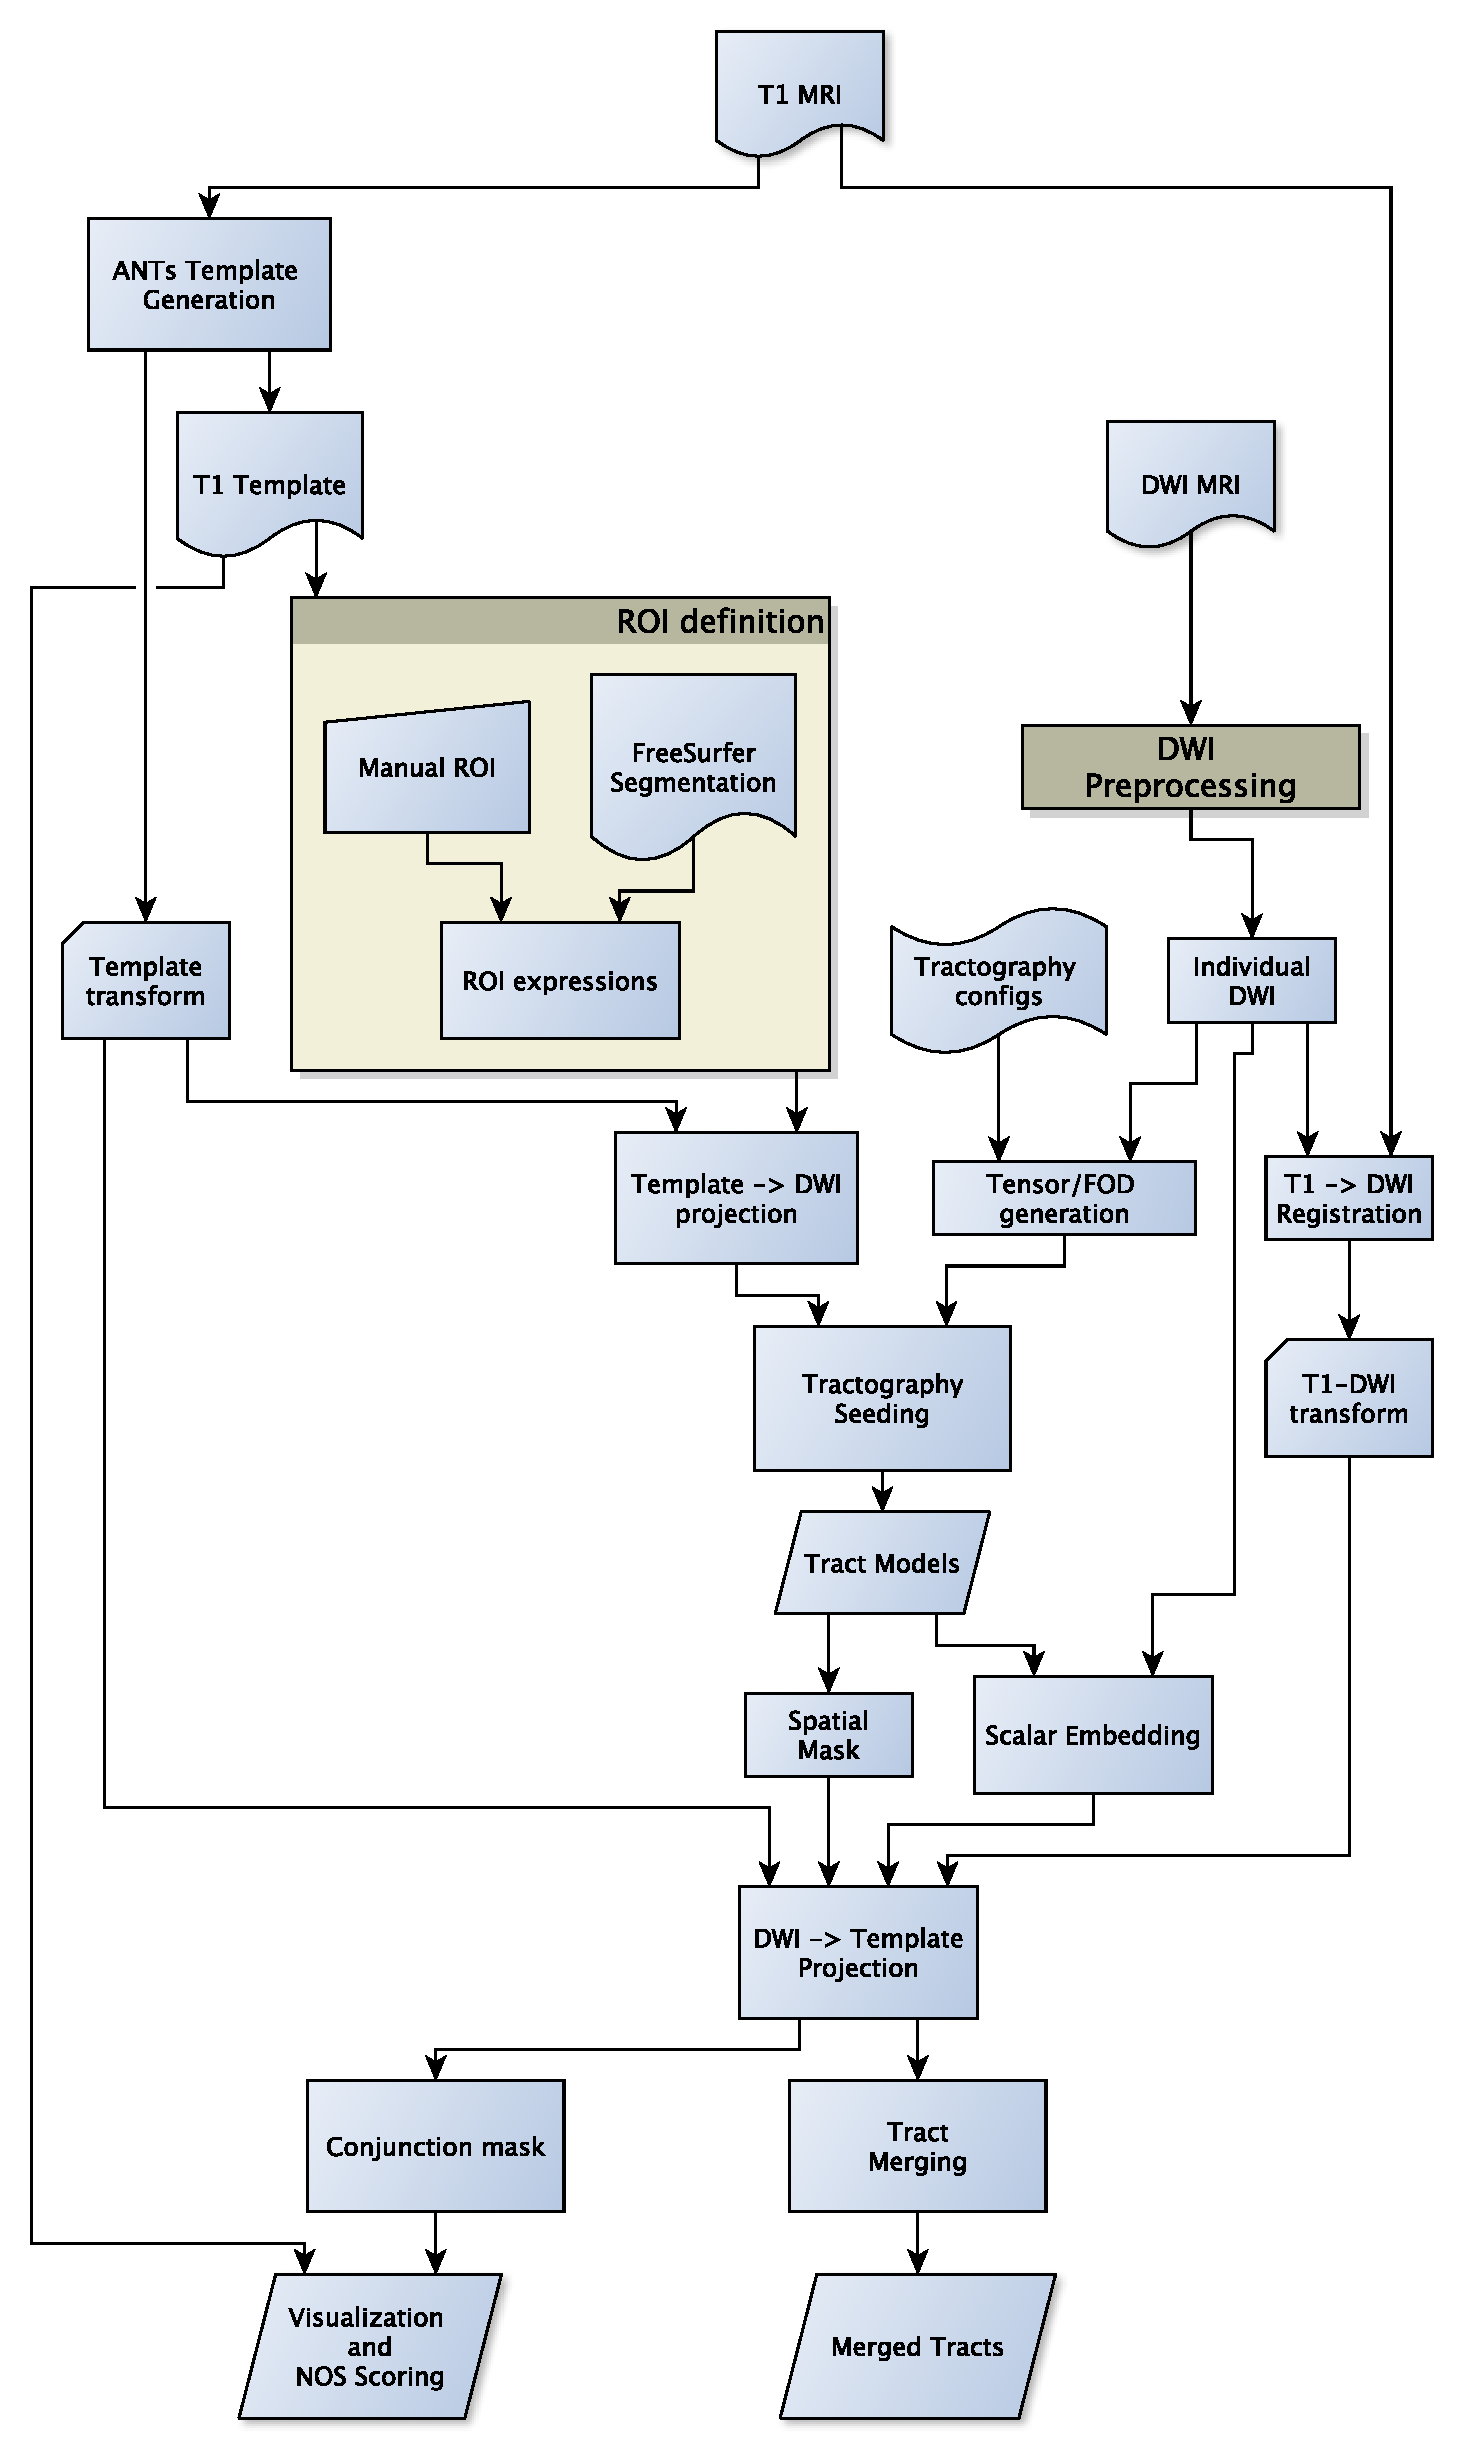
\includegraphics[width=0.8\linewidth]{figure1.pdf}
\caption{Flow diagram of the SAGIT group tractography framework. The SAGIT framework is designed to be fully configurable and extensible.}
\label{fig:SGfigure1}
\end{figure}

\afterpage{%
    \clearpage% Flush earlier floats (otherwise order might not be correct)
    \thispagestyle{empty}% empty page style (?)
    \begin{landscape}% Landscape page
    
\begin{figure}[p]
\centering
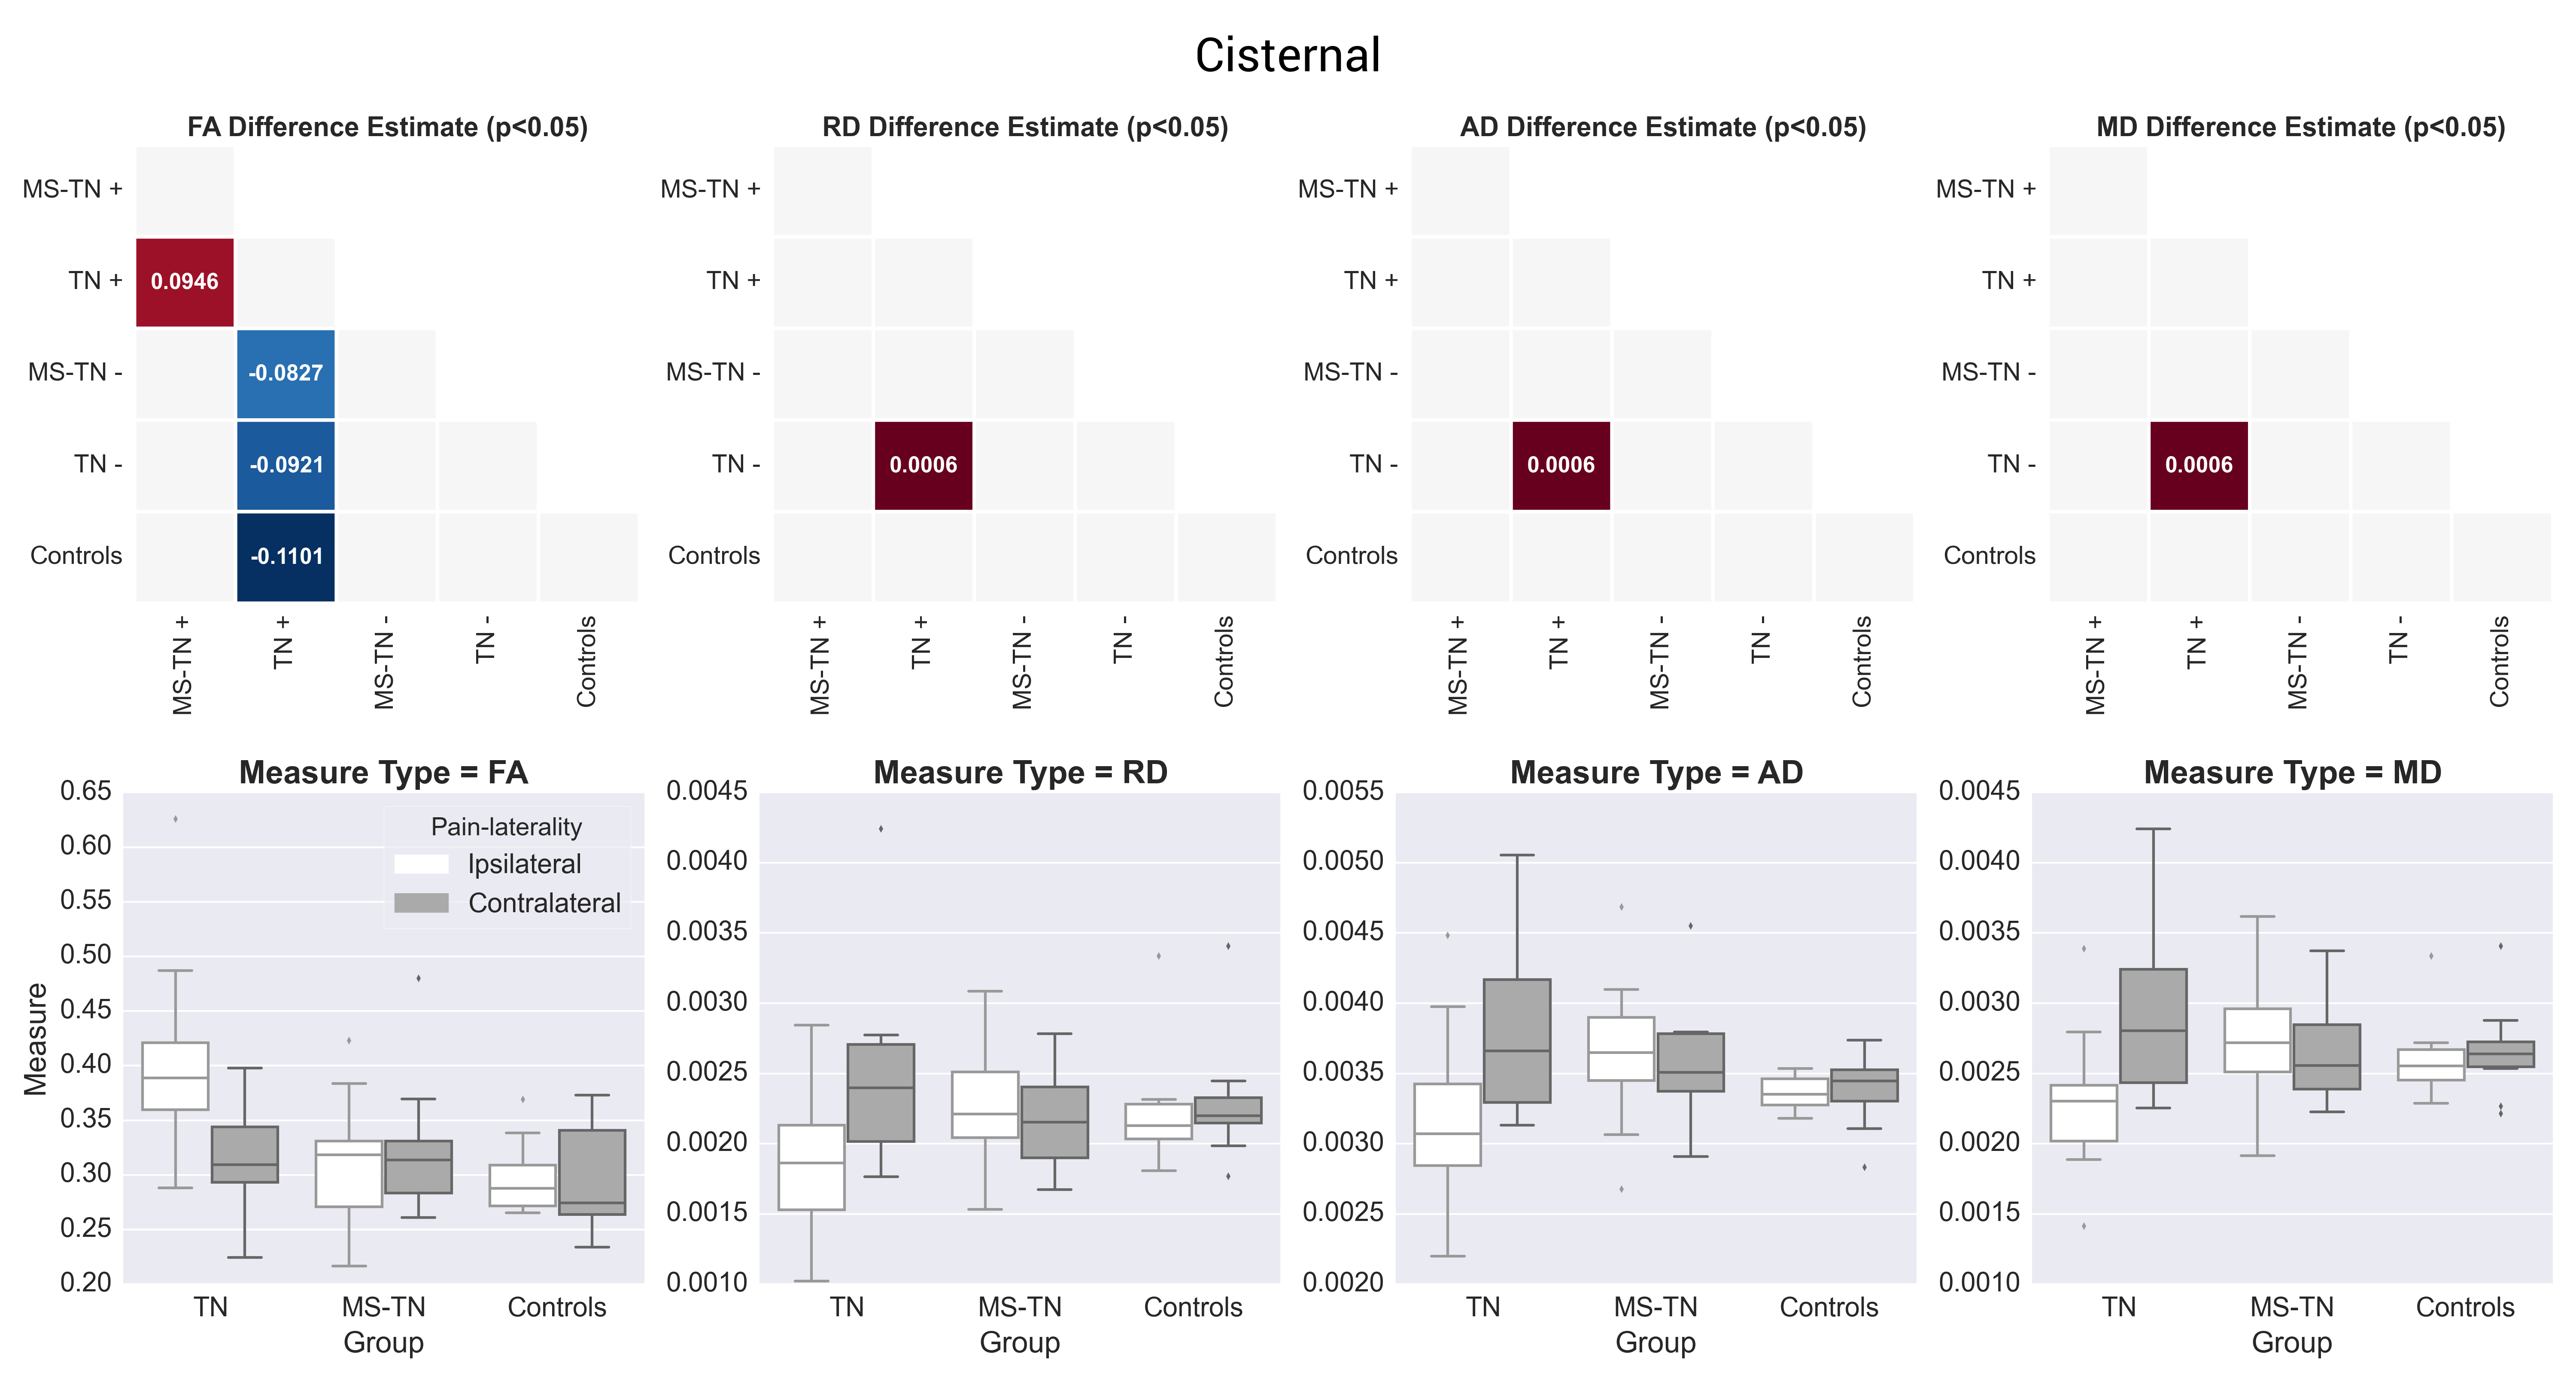
\includegraphics[width=\linewidth]{figure4.png}
\caption{Examples of NOS scores of different conjunction images: The figure shows the coronal view of the left red nucleus tractography projections, as produced by different algorithms. The NOS score correlates closely with the visual colour scale. It can also resolve visually similar comparisons, such as the rating between XST and CST deterministic results.}
\label{fig:SGfigure4}
\end{figure}
	\end{landscape}
	\clearpage
}

\section{Results}

The fornix was shown to be consistent across the different algorithms. The visual report (Figure 2; the complete visual report can be found in supplemental) suggested that the subregions of the fornix were consistently delineated. The merged fornix tracts (Figure 3) showed different patterns of streamline distributions. CST$_{prob}$ and XST both showed wide spread streamline dispersions, while CST$_{det}$ and particularly DTT were limited to the region of the fornix. The fornix ratings (Figure 5) showed essentially no variability between raters.  The fornix NOS scores (Figure 6) similarly were consistent across the algorithms with little variability. Both filtered and unfiltered ratings were identical. 

For the CN VII/VIII, CST$_{prob}$, CST$_{det}$ and XST were all able to delineate the cranial as well as brainstem segments of the nerve (Figure 2). CST$_{prob}$ however also delineated much of the cerebellum. DTT by Slicer was not able to delineate the brainstem portions of the fibre and therefore was scored lower than the other methods. These differences in delineation can be more clearly seen in the merged tracts (Figure 3), where the XST also showed further lateral delineations of CN VII/VIII. In unfiltered tractography, there was much more inter-rater variability for all except CST$_{prob}$. CST$_{det}$ and XST also showed lower average rating when unfiltered (Figure 5). The NOS showed similar trend where DTT resulted in the lowest score (Figure 6). The NOS also showed higher score for CST$_{det}$ when comparing to XST. There were no notable changes in NOS scores in unfiltered tractography. 

For CN X, CST$_{prob}$ was rated the highest with no inter-rater variability. CST$_{det}$ and XST resulted in more rating variability and a lower average score (Figure 5). CST$_{prob}$ visually showed delineations that extended into the ipsilateral higher brain regions even with filters (Figures 2, 3). DTT showed the worst reproducibility, although its anatomy was recognizable in a small number of individuals.  In unfiltered tractography, CST$_{det}$ and XST showed reduced variability, and visually showed delineations of ascending and brainstem projects. DTT also showed improved ratings when unfiltered. NOS scores (Figure 6) for both filtered and unfiltered CN X tractography similarly showed an overall increase in score with unfiltered tractography. 

For the red nucleus projections, visually CST$_{prob}$ showed the most consistent reproducibility of the decussation (Figure 2, Figure 3), with XST showing higher reproducibility over CST$_{det}$. DTT failed to delineate the pathway and instead delineated an erroneous path that decussated at the corpus callosum. CST$_{prob}$, CST$_{det}$ and XST resulted similar ratings, with unfiltered tracts showing lower rating and higher variability. DTT had the lowest rating, and very high variability (Figure 5). NOS score of the red nucleus projections highlighted the stronger performance of the CST$_{prob}$ over the other algorithms, and XST result was scored higher than CST$_{det}$ (Figure 6). The NOS scores of unfiltered tracts were notably higher for all algorithms, as the resulting tracts seemed to delineate much of the cortical spinal projections. 

 The optic radiation showed the greatest reproducibility with CST$_{prob}$, where the Meyer’s loop could be seen in the result (Figure 2, Figure 3). CST$_{det}$ and XST showed low reproducibility of less than 20\%, and DTT failed to delineate any structure on the right side (see supplemental). The ratings reflected the observation (Figure 5), with CST$_{prob}$ having the full rating. CST$_{det}$ was rated higher in filtered tractography, while XST was rated higher when unfiltered. DTT also showed higher ratings when unfiltered. NOS score characterized the drop-off in reproducibility in filtered tractography for the deterministic methods (Figure 6), and the trend of rating under filtered tractography matched well with the ratings. NOS scores for unfiltered tractography however showed little match with ratings. 
 
The auditory radiation was the least reproducible region. In filtered tractography, although CST$_{prob}$ showed high reproducibility in tractography (Figure 2, Figure 3), it was not clear if its delineation was correct. Visually there were wide spread area of false positives towards the occipital and anterior temporal lobe. The deterministic methods all showed poor ability to reach the Heschl’s gyrus. DTT was completely unable to produce any structures at all. For filtered ratings,  CST$_{prob}$ was the highest, and with XST rated higher than CST$_{det}$ (Figure 5). DTT scored zero due to the lack of delineated structures. When unfiltered, all algorithms showed widespread false positives in the hemispheres. Unfiltered ratings were over all higher than filtered ratings. NOS scores’ trends for filtered tractography matched well with ratings, but also highlighted the large differences in reproducibility (Figure 6). While NOS scores under unfiltered tractography did not correlate with ratings. 

Linear regression of rater scores against NOS (Figure 7) showed significant (p\textless0.05) correlation of the two sets of scores in filtered tractography. However correlations were not significant (p\textgreater0.05) for unfiltered tractography. It can be observed that NOS score in unfiltered tractography agrees well with visual intuition, however rater variability and anatomical reports suggested greater false positives when presented with unfiltered results.  

\afterpage{%
    \clearpage% Flush earlier floats (otherwise order might not be correct)
    \thispagestyle{empty}% empty page style (?)
    \begin{landscape}% Landscape page

\begin{figure}[p]
\centering
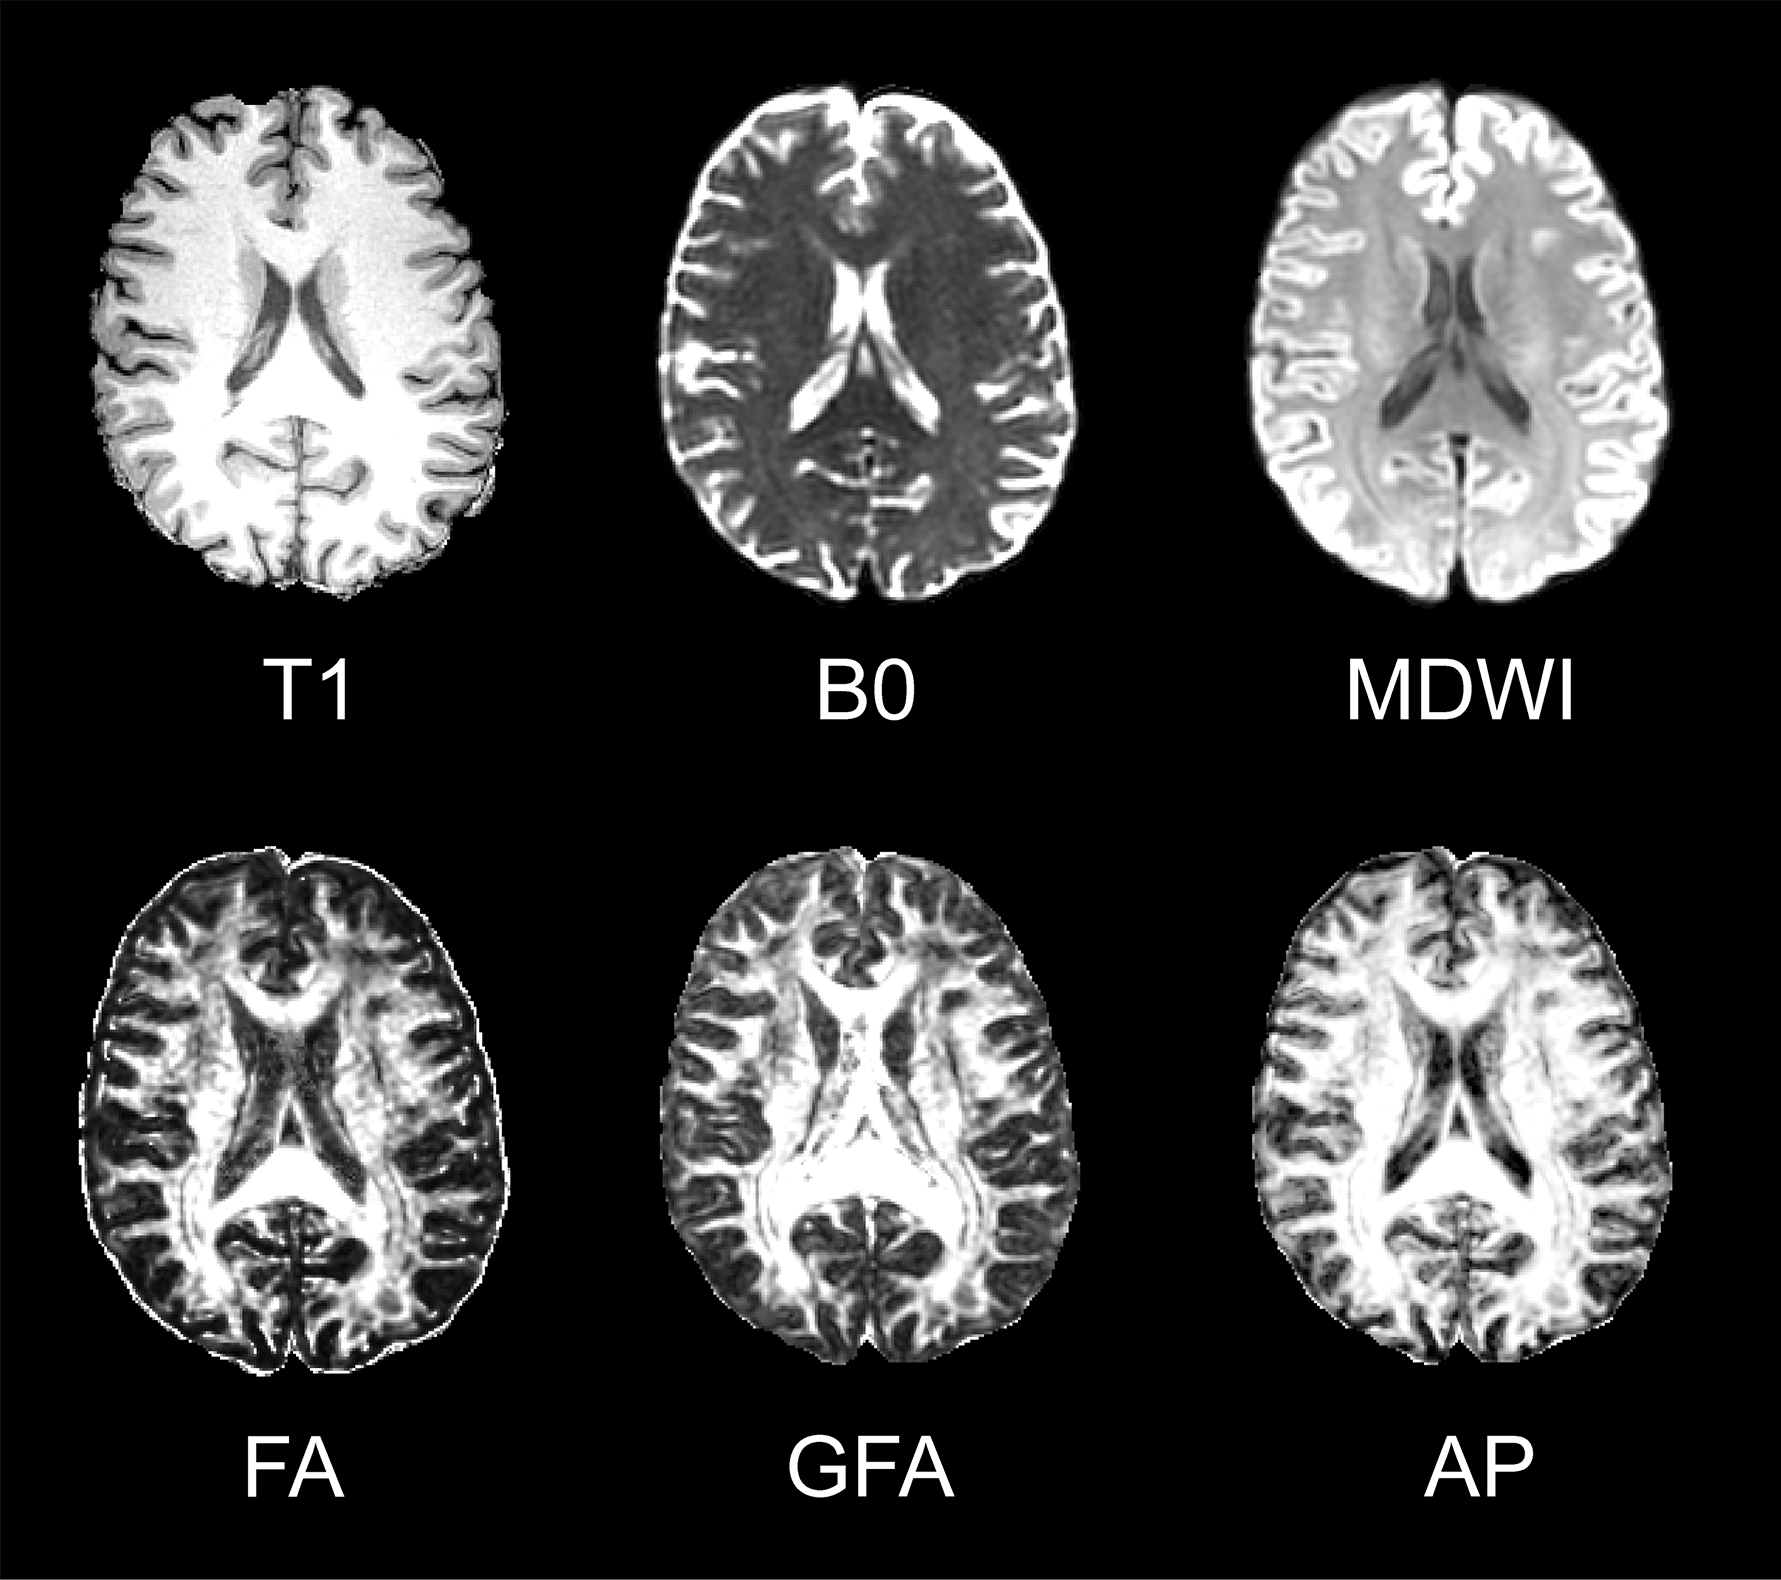
\includegraphics[width=\linewidth]{figure2.png}
\caption[Example of the auto-generated visual panels.]{Example of the auto-generated visual panels. The panels that best represent the resulting anatomy are compiled. For anatomical reference, the best representative anatomy image slice is composed with the tract conjunction map. The colour scale of the conjunction image represents the percentage reproducible for each region, where 1=100\%. For each algorithm (rows), different visual perspectives are created. Together 6 different anatomies were delineated (columns). To see the full visual reports generated, please see supplemental.}
\label{fig:SGfigure2}
\end{figure}

    \end{landscape}
    \clearpage% Flush page
}

\afterpage{%
    \clearpage% Flush earlier floats (otherwise order might not be correct)
    \thispagestyle{empty}% empty page style (?)
    \begin{landscape}% Landscape page
\begin{figure}[p]
\centering
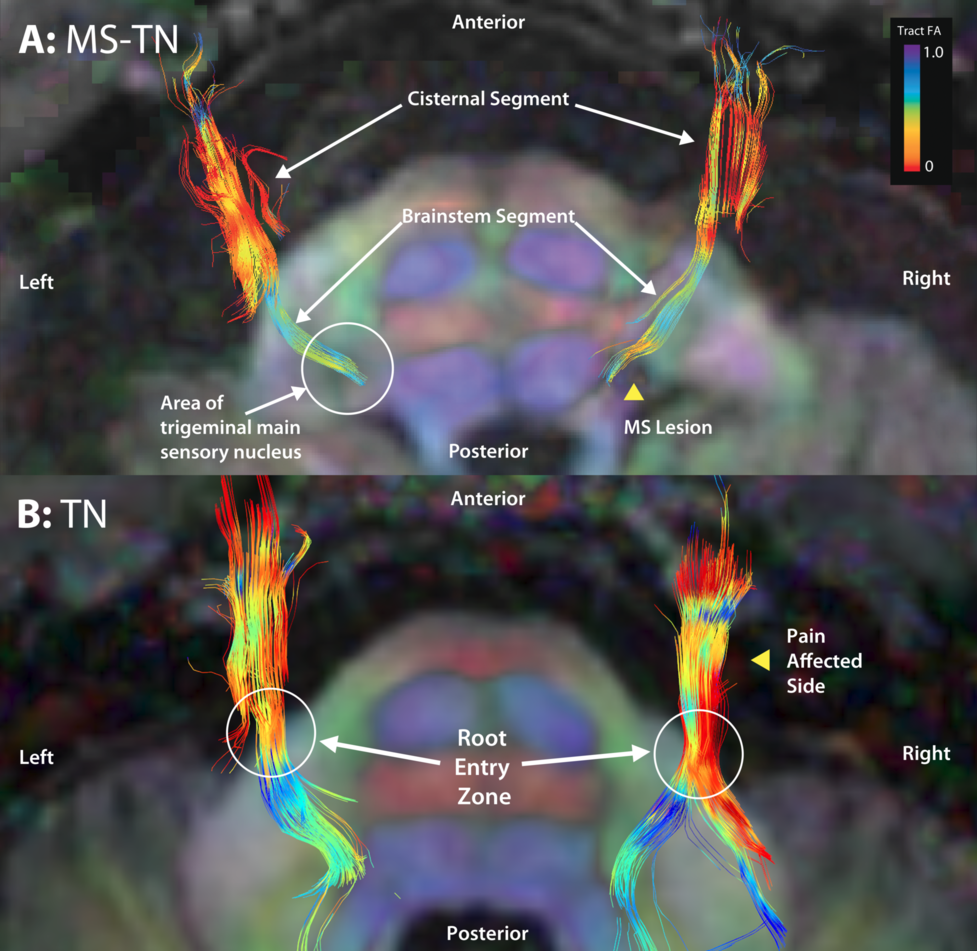
\includegraphics[width=0.9\linewidth]{figure3.png}
\caption[Example of merged tractography models for each of the techniques and anatomy.]{Example of merged tractography models for each of the techniques and anatomy. The fornix is coloured to distinguish tracts from each of the 42 subjects, in order to demonstrate the effect of combining the group data. The other anatomies are coloured by FA intensity. The specific FA measures from each point were sampled from their native DWI space before tractography deformation. The grouping of the similar FA measures across the subjects show that the registrations were accurate. The Red Nuclei shows different metrics (FA and AD) depending on lateralization, in order to highlight the pontine decussation.}
\label{fig:SGfigure3}
\end{figure}
    \end{landscape}
    \clearpage% Flush page
}

\begin{figure}[ht]
	\centering
	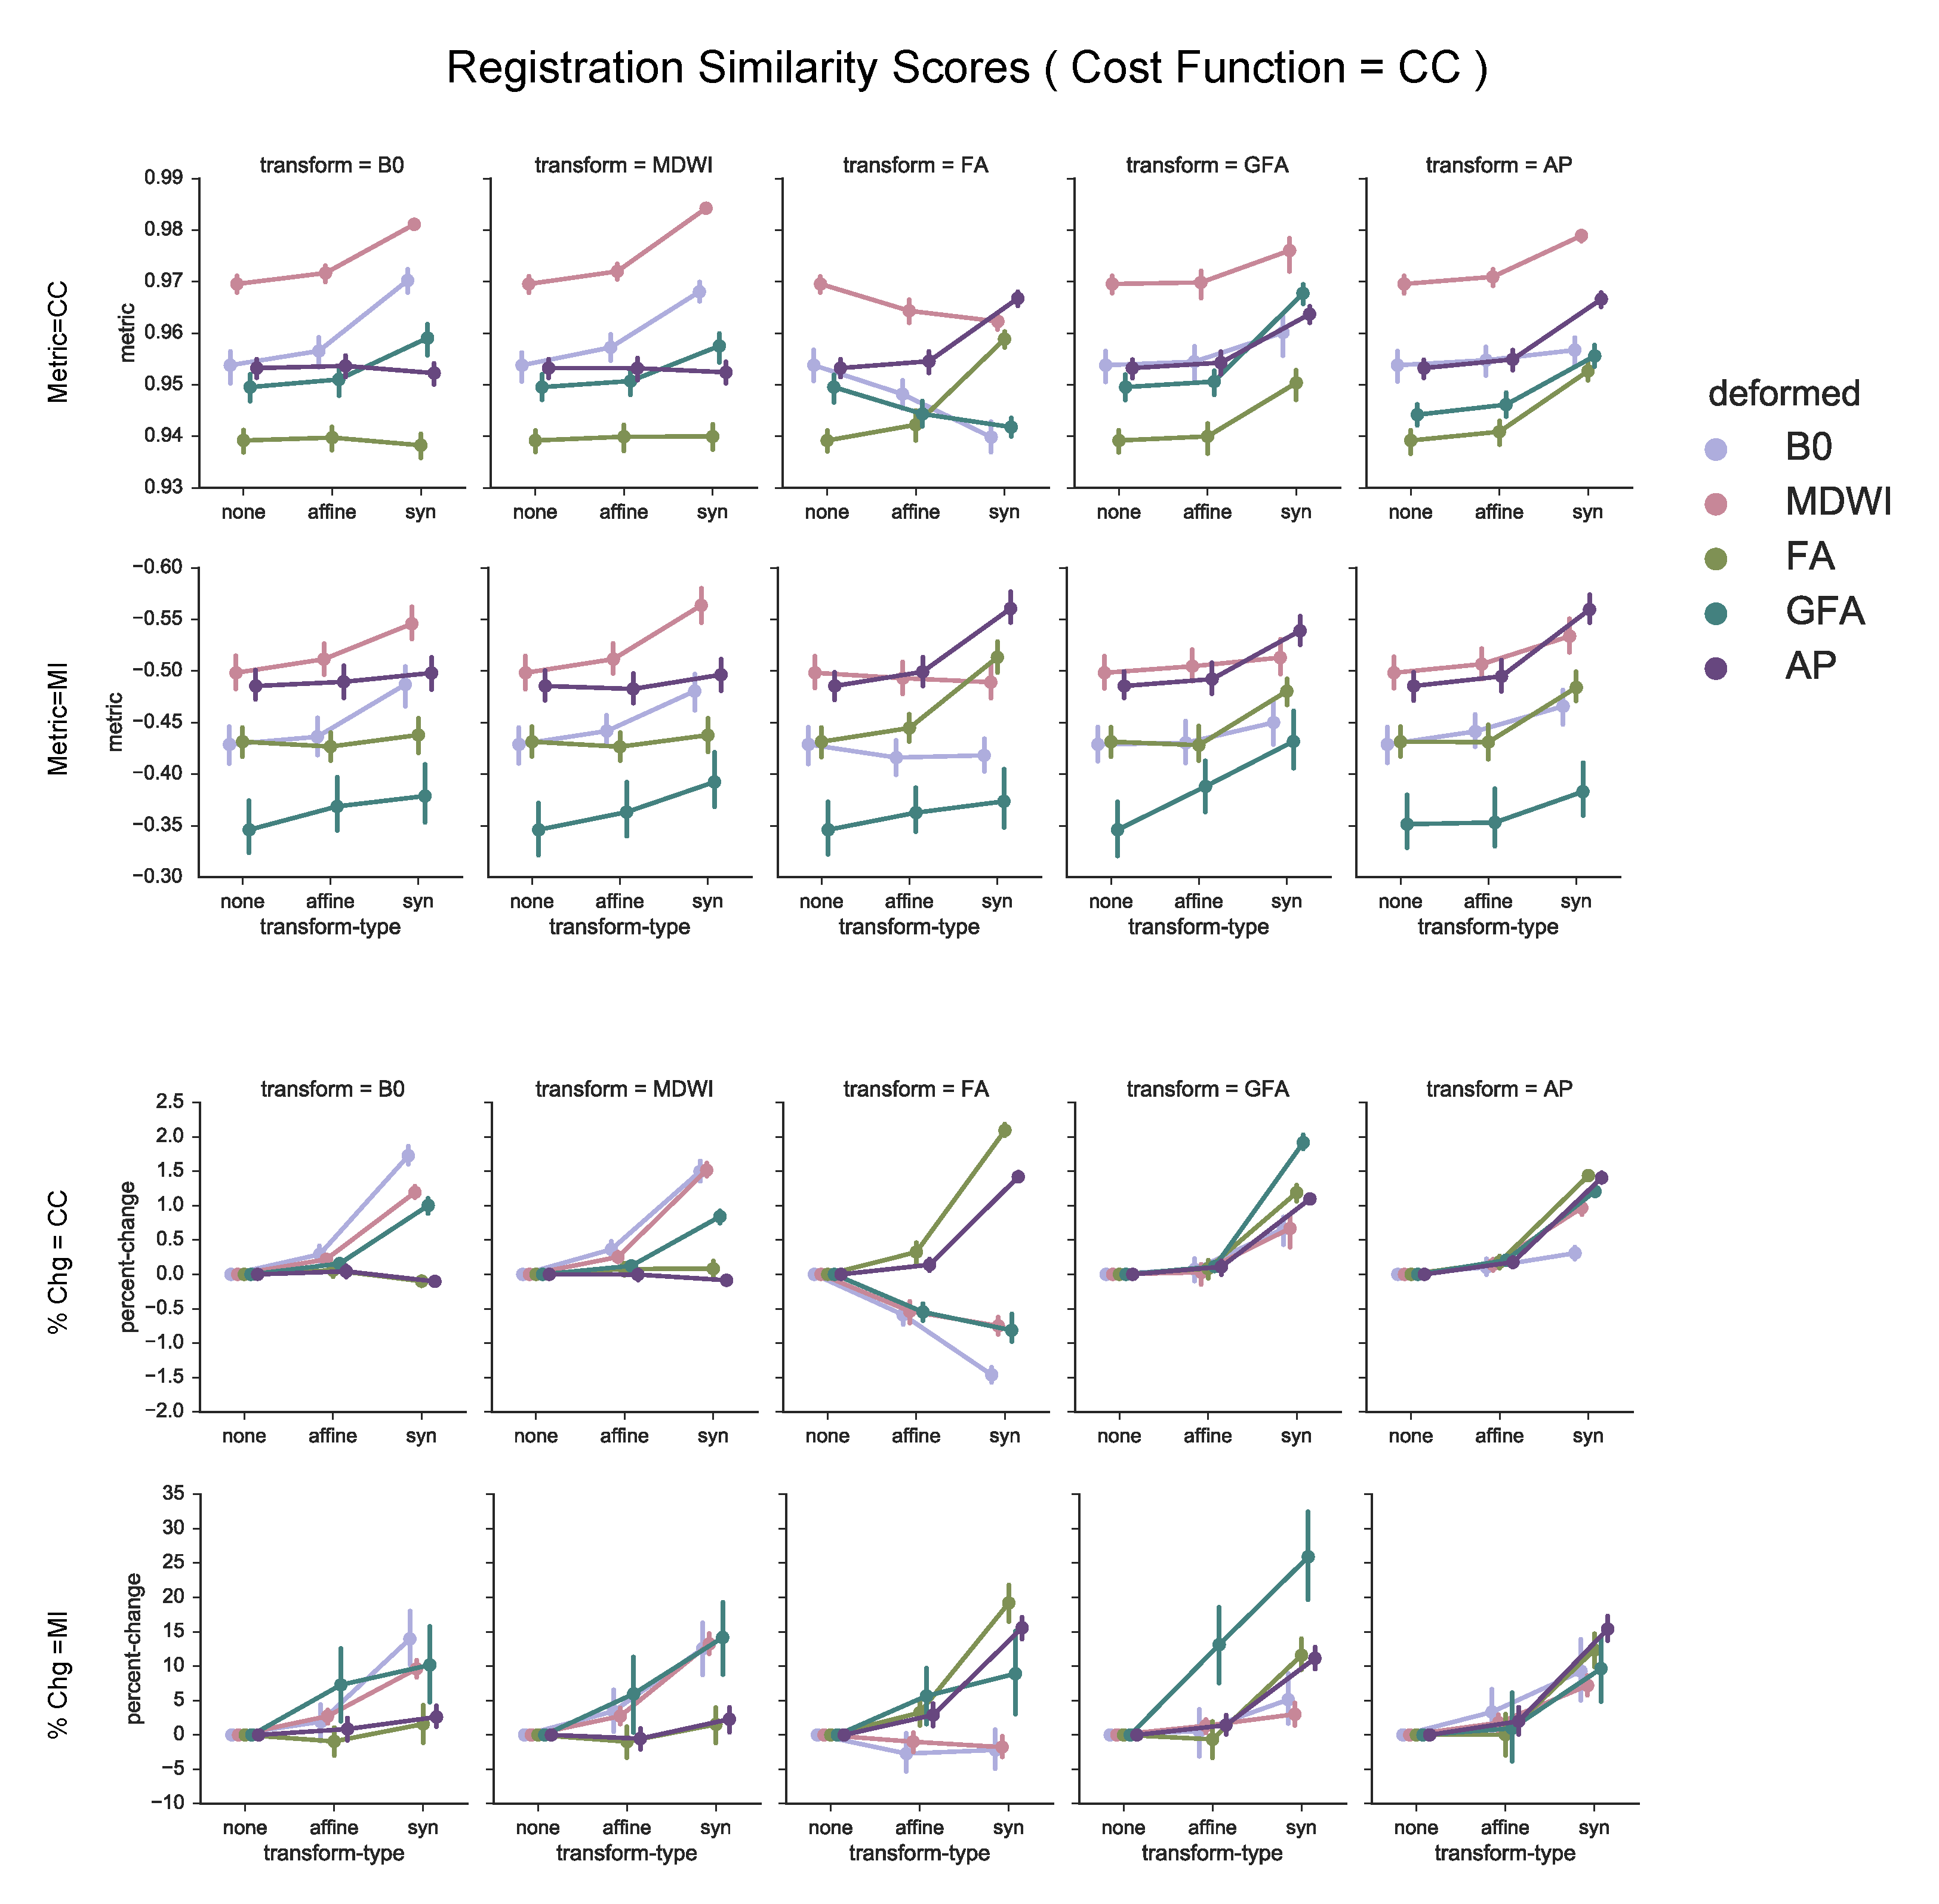
\includegraphics[width=\linewidth]{figure5.pdf}
	\caption[Normalized anatomical scores as rated by experts.]{Normalized anatomical scores as rated by experts. The error bars denote standard deviations of the ratings. The fornix serves as the control anatomy, therefore the represented filtered and unfiltered image are identical. It can be observed that unfiltered anatomy increases rater variability in some and decrease in others.}
	\label{fig:SGfigure5}
\end{figure}

\begin{figure}[ht]
\centering
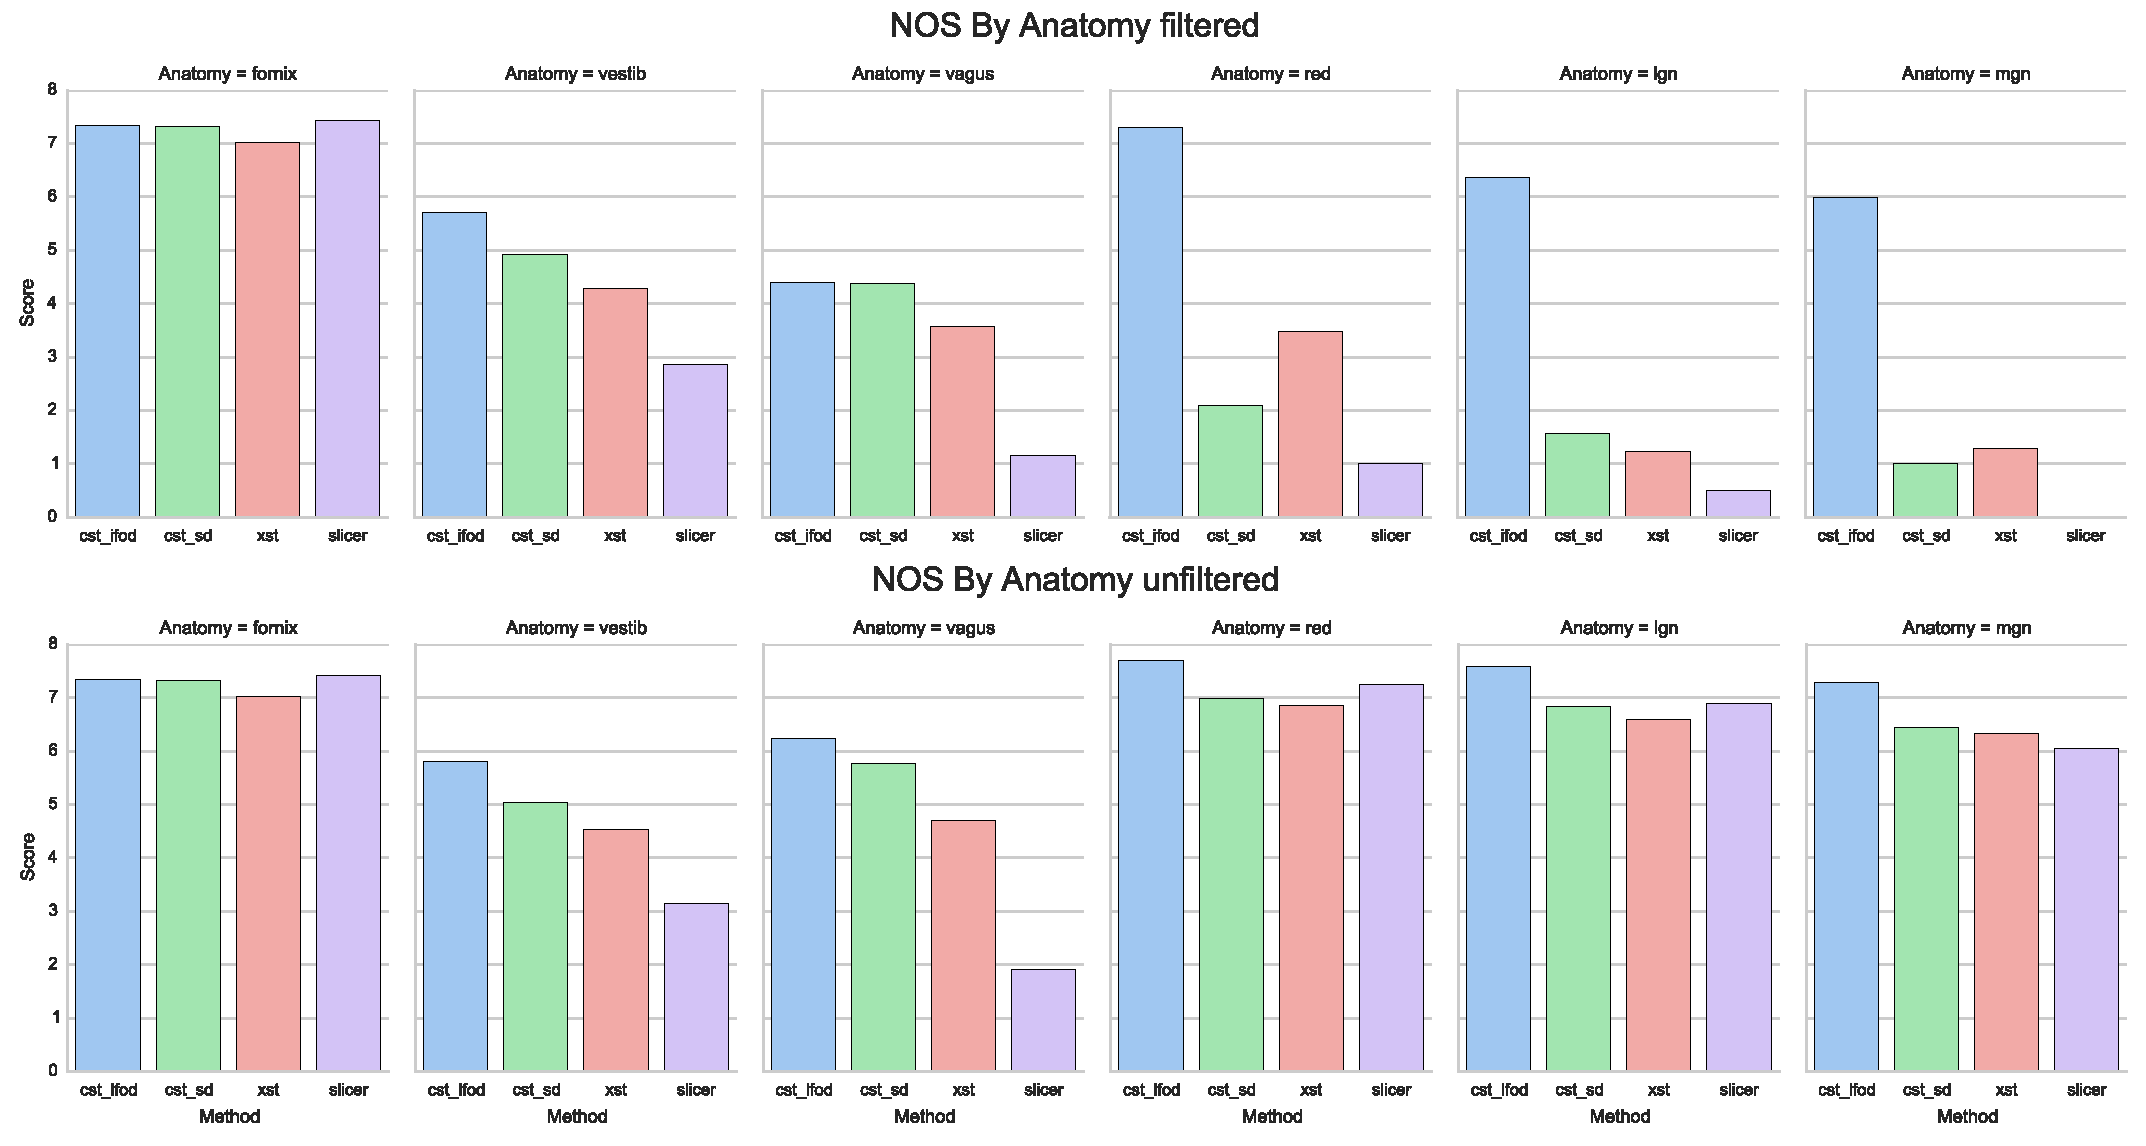
\includegraphics[width=\linewidth]{figure6.pdf}
\caption{NOS scores for each anatomy. It can be noted that having ROI filters severely reduces reproducibility in deterministic methods.}
\label{fig:SGfigure6}
\end{figure}

\begin{figure}[ht]
\centering
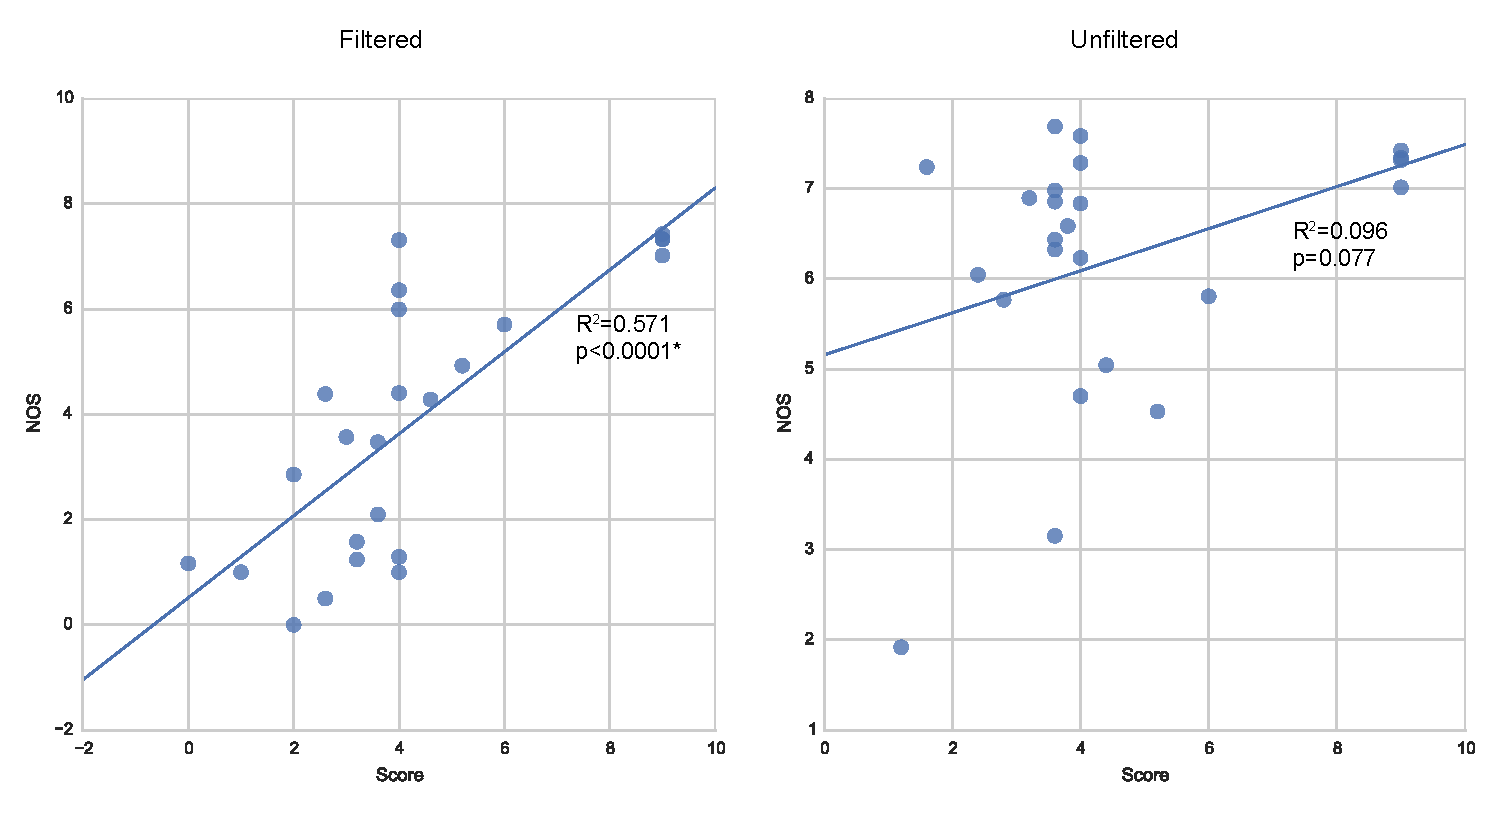
\includegraphics[width=\linewidth]{figure7.pdf}
\caption{Correlation between rating scores and NOS. Filtered tractography NOS is significantly (p\textless 0.05) correlated with ratings. However unfiltered tractography show no significance.}
\label{fig:SGfigure7}
\end{figure}

\section{Discussion}

The present study performed automated group tractography generation and collation report on 6 sets of neuroanatomy in 42 subjects using 4 different types of tractography algorithms. The proposed automation pipeline performed with great reliablity. We have designed the automated pipeline to offer the ability to generate and collate tractography on a large scale. The key benefit of this approach is the vastly improved inter-subject tract reproducibility as a result of ROI filtering, and speed for tractography data generation. The method offers flexibility for researchers in ROI placements and parameter control for these tractography algorithms. The merged tractography permits additional analysis of the group-based anatomical reconstructions, and the auto-generated visual reports also reduce data confusion and improve research efficiency. 

The most critical component of the pipeline is the reliability of image registrations. For this purpose, we picked ANTs since it is state-of-the-art and widely tested and deployed in numerous neuroimaging studies \cite{Avants2011,Klein2009}. For T$_1$ to DWI co-registration, we used mean diffusion weighted image (MDWI) as the registration intermediate. MDWI appears to be a reliable T$_1$-DWI co-registration intermediate in the absence of reverse-blip DWI acquisitions \cite{Chen2015b}. Future studies can also potentially improve T$_1$-DWI co-registration, for example with the possible use of anisotropic power image\cite{DellAcqua2014}. 

We have deployed the pipeline to the task of delineating 6 sets of neuroanatomy from clinical DWI data. The anatomies were chosen to test the limits of the SAGIT pipeline as well as the tractography algorithms. These anatomies are often shown in an existing atlas, and contain curving projections that are difficult to delineate, but are nevertheless well defined and contain clear anatomical landmarks for ease of judgment. In total we included: two sets of cranial nerves (CN VII/VIII and CN X) for their small but precise anatomy; rubrocerebellar projections of the red nucleus, due to the difficulty of imaging the pontine decussation; optical radiation for its well defined landmarks and the Meyer's loop, which is difficult to image; auditory radiation, which is particularly difficult due to its course, that passes through a 3-way crossing in temporal lobe. The fornix serves as the control anatomical structure. We have previously studied fornix sub-region anatomies extensively \cite{Chen2015c}, and it is a popular anatomy to showcase the ability of new tractography algorithms due to the curvature of the forniceal crura \cite{Garyfallidis2014}. 

It can be observed that results of averaged tractography image conjunction across a group are visually similar to probabilistic tractography in an individual, and that the group junction image seems to stabilize as the number of subject increase. It can be argued that the conjunction image captures the probable volume across a sampled population for a particular neuroanatomy in the template space. Their exact similarity and differences from probabilistic tractography at a group level should be explored in future studies. Additionally, the fidelity of the merged anatomy is often higher than what would be available from an individual. The result supports the validity of this technical approach. It is possible that the resulting average delineations can be used to generate population-specific anatomy atlases. It's also possible to use fibre density images rather than binary mask for conjunction. However the result of an average fibre density image is difficult to interpret, and therefore should be explored in future studies.

When attempting to judge tractography delineation quality, human experts often are able to assess a particular delineation by visually identifying known anatomical priors. Direct tractography visualizations suggest that wide streamline dispersions often obscure anatomical details in visualizations, making anatomical assessment difficult (figure 3). Therefore, image conjunctions offer better ability to assess reproducibility than direct tractography renderings alone. We aimed to develop an automated assessment of tractography reproducibility, since a) researchers are often prone to judgment bias when exposed to large number of tractography results, and that subtle differences in results are often hard to distinguish, and b) in an automated pipeline, the assessment score is necessary to allow iteratively fine tuning of tractography parameters. Since current neuroimaging techniques are not yet able to reliably classify neuroanatomy from tractography or image-based morphology, it is desirable for a computing pipeline to optimize and present the most reproducible tractography delineating across a population based on a particular set of ROIs as a first step. Subsequent anatomical assessment can then be made by a human expert, and the appropriate changes in ROI filter strategy can be made. This approach allows researchers with strong neuroanatomy backgrounds, but are less technically inclined, to make better judgments when performing group tractography. 

The NOS and rater scores correlated significantly in filtered tractography. There was, however, little correlation in the case when tractography were unfiltered. The NOS scores are closely related to the change in visual scale of the averaged result; thus, suggesting that human ratings assessments of filtered tractography are well encapsulated by the NOS score, whereas the human decision factors for unfiltered tractography are more complex. Since the rating questionnaire is based on yes/no decisions on sub-anatomy identification, it is possible that the raters preferred to err more on false-positives than risking false-negatives, and this is what contributes to the differences in unfiltered tractography ratings. This means that human rating can become unpredictably biased with different filtering parameters and a more stable rating metric such as NOS may be more desirable.  

For the specific tractography algorithms, CST$_{prob}$ produces the highest ratings, and performs particularly well in the optical radiation. It also results in more false-positives. This is most evident in CN VII/VIII and CN X results. In these cases the cranial nerve anatomies are very specific and local, and yet CST$_{prob}$ produces more false-positive projections to distant regions. In the fornix there are also erroneous tract extensions into the corpus callosum. Deterministic methods in comparison are more conservative and therefore result in lower scores. They perform well when the anatomy is regional and has finer features. Both CST$_{det}$ and XST performed well with cranial nerves. XST is able to image the rubro-cerebellar pontine decussation with more reliability than CST$_{det}$. While CST$_{prob}$ decussation delineation shows the highest reproducibility, it also produces wider projection coverage that’s harder to interpret. The low DTT score is not surprising, as the single-tensor's inability to resolve crossing-fibres is well known. Based on the result of the study, we recommend the use of CST$_{prob}$ for tasks in which the target anatomy is well defined and false positively can be easily recognized , or when interhemispheric and long projection distances are desired. For exploratory tractography, where filtering locations are not well defined, or when the anatomy features are close together, deterministic methods are recommended. When comparing CST$_{det}$ and XST, it appears that XST is more conservative and thereby results in less false-positives. It also has better ability in resolving hemispherical decussations, as evident by the results of the rubro-cerebellar projections. In practice the two methods are very close in performance. Note however that the comparison is not exhaustive of the possible parameter combinations on either method, and therefore automated tuning of the parameters can answer this question more definitively. 

It is evident from this study that there is no single tractography algorithm that is superior in all aspects. The recent Tractometer challenge \cite{Neher2015}, which compared a wide range of tractography algorithms, including DTT and CST on a high resolution DWI phantom, has come to the same observation. It is clear that algorithm choice is highly task-dependent. Given that vast number of neuropathologies are not well understood, there is often no available ground truth of neuroanatomical measure in the clinical environment from which to form priors regarding algorithm performance.  Automatic tuning of tractography parameters in order to maximize anatomy and population-specific reproducibility, and thereby allowing task-specific tractography algorithm recommendations is a highly desirable future direction. The SAGIT platform and NOS score are a first step towards this goal. 

\subsection{Limitations}
For this study the DWI images were acquired at 0.94$\times$0.94$\times$3 $mm\textsuperscript{3}$ voxel resolution. The dataset was acquired for the purpose of cranial nerve visualization on a 3T GE HDx MRI with 8-channels head coil, and is therefore incapable of less than 2.6 mm isovoxel DWI resolution at a clinically acceptable scanning time. For example, the average trigeminal nerve, one of the larger cranial nerves, has a diameter of about 2 mm, as of such we compromised on an anisotropic voxel resolution to gain in-plane resolution. We believe our findings is novel for the application of clinical tractography delineations in less than ideal conditions. 

The limit of the NOS score is closed tied to the performance of its associated tractography algorithm. An algorithm and its associated parameters may consistently produce the wrong result in all subjects and produce a high NOS score, or it may produce no results, and result in a NOS score of 0. Both of these cases are regular occurrences in single-subject tractography analysis. With merged tractography, it is easier to recognize such faults. This is because in practice, incorrect tract path are often the result of imaging anomalies or algorithm limit, and are unstable across a population. This can be observed as a general trend in Figure 3, for example where DTI delineation of the rubrocerebellar tract is clearly incorrect, and results in low NOS score. Therefore, NOS score is capable of characterizing the uncertainty as a result of low algorithmic performance. In the case of false positives that are highly consistent, SAGIT can help researchers making more informed judgement.

\section{Conclusions}

In this study, the SAGIT platform was created as an automated group tractography software platform that incorporated existing and proven dMRI practices, in order for group-wise dMRI to be more accessible to researchers. The tractography results demonstrated reliable and consistent performance of SAGIT across multiple subjects and techniques. By deploying SAGIT on 42 subjects, we quantifiably demonstrated that merged tractography is able to demonstrate algorithmic differences at a group-level. CST$_{prob}$ is prone to false-positives, and thereby is suitable when the targeted anatomy is well known. CST$_{det}$ and XST are more conservative, but have more trouble resolving hemispherical decussation and distant crossing projections. The NOS score shows significant correlation with rater score for filtered tractography. Therefore it may be used for automated ratings of group tract results. As no single algorithm seems to be suitable for all anatomical tasks, it would be useful to consider using a mix of algorithms for different anatomical segments. Finally, we have demonstrated that merged tractography is a promising group-wise tractography analysis approach. 






\graphicspath{{thesis/images/tn-gp-sagit/}}

\chapter{Study IV: Trigeminal Neuralgia Diffusivities using Gaussian Process Classification and Merged Group Tractography}
\chaptermark{Study IV}
\label{section:study4}

\bibentry{Chen2018tnsagit}

\section{Abstract}
\textbf{Introduction:}  Imaging of trigeminal neuralgia (TN) has demonstrated key DTI based diffusivity alterations in the trigeminal nerve but imaging has primarily focused on the peripheral nerve segment, since technical limitations have  prevented us from assessing the trigeminal nerve and its connections in the central nervous system. We apply fully-automated group white-matter tractography to image the trigeminal sensory pathway and machine learning classification using a Gaussian Process (GP) classifier to pinpoint key white-matter diffusivity changes that maximally differentiate TN subjects from healthy controls. 

\textbf{Methods:} We used SAGIT based group merged tractography to study 36 sex-matched TN subjects (right-sided pain) and 36 controls, examining the following trigeminal related white matter pathways: trigeminal nerve (CN V), pontine decussation (TPT), and thalamocortical fibers (S1). GP classifiers were trained by scrolling a moving window over CN V, TPT, and S1 tractography centroids. Fractional anisotropy (FA), generalized FA (GFA), radial diffusivity (RD), axial diffusivity (AD), and mean diffusivity (MD) metrics were evaluated for both groups, analyzing TN vs. control groups and affected vs. unaffected sides. Classifiers that performed at greater-or-equal-to 70\% accuracy were included.

\textbf{Results:} GP classifier consistently demonstrated bilateral trigeminal changes, differentiating them from controls with an accuracy of 80\%, even though the clinical expression of pain was strictly unilateral. Affected and unaffected sides could also be differentiated from each other with an accuracy of 75\%. Assessment of the trigeminal subregions demonstrated that the segments in affected CN V differ from controls from the region of the REZ and distally. Bilateral TPT could be distinguished from controls with at least 85\% accuracy while TPT left-right classification achieved 98\% accuracy. Bilateral S1 could be differentiated from controls, where the affected S1 RD classifier achieved an accuracy of 87\%.

\textbf{Conclusions:} This is the first study in TN that combines group-wise merged tractography, machine learning classification using GP, and analysis of the complete trigeminal pathways from the the trigeminal peripheral fibers to S1 cortex. This analysis demonstrates that TN is characterized by bilateral changes throughout the trigeminal pathway compared with healthy controls, as well as changes between clinically affected and unaffected sides. The combination of group tractography and machine learning have proven to be a powerful approach for the study of white matter diffusivities.

\section{Introduction}
\subsubsection{Trigeminal Neuralgia}
Trigeminal neuralgia (TN) is a debilitating facial neuropathic pain syndrome characterized by paroxysmal and shock-like pain in one or more divisions of the trigeminal nerve (The fifth cranial nerve, CN V) branches. TN manifests most commonly as classic (also called idiopathic TN), or secondary to a range of neuropathology, including tumors such as meningiomas \cite{Cheng2008}, trigeminal schwannomas \cite{Miller2008}, and most notably multiple-sclerosis (MS) \cite{Cruccu2009,VanderMeijs2002,Nick2012}. The pathophysiology of classic TN is thought to be vascular compression at the root of the CN V nerve entry zone (NEZ) \cite{Linn2011,Love2001}, although classic TN can also occur without evidence of vascular compression \cite{Lee2014}. While the focus of the study of TN has been primarily the peripheral segments of the trigeminal nerve, we recently compared TN and MS-TN diffusivity differences in four segments of the CN V, including at the level of the pons \cite{Chen2016a}, and confirmed that brainstem CN V diffusivity is altered in MS-TN. Similarly, we demonstrated, using multi-tensor tractography, that altered diffusivity at the level of the pons prognosticates treatment non-response \cite{Hung2017}. It appears therefore that TN is associated with unique peripheral abnormalities and brainstem related central abnormalities. 

Investigation of potential gray and white matter findings in TN has demonstrated that there are key abnormalities in areas important for discrimination and modulation of pain, including the thalamus, basal ganglia, primary somatosensory cortex, primary motor cortex, orbitofrontal cortex, cingulate cortex, and insula \cite{Desouza2013c, Desouza2013}.

The trigeminal sensory system involves both discriminative touch and pain pathways \cite{Henssen2016}.  Pain and discriminitive touch stimuli trigger innervations of the three trigeminal nerve branches (V1, V2, and V3) in the head and face, these primary affrents converge and form the trigeminal root gangion (TRG) (also known as Gasserian, or semilunar ganglion) in the middle cranial fossa. The discriminative touch afferents then course through the cisternal segment of CN V, enter the pons, and synapse onto the primary trigeminal sensory nucleus, after which they project to the contralateral VC thalamus and the S1 cortex. The nociceptive pathway synapses caudally onto the trigeminal spinal nucleus, decussates at the level of the medulla and spinal cord. The pathway merges with the discriminative sensory pathway and ascend as the contralateral trigeminal lemniscus, and also project to the contralateral VC thalamus. The pain pathway also projects to the medial nucleus of the thalamus, after which it courses towards the fibers of the cingulate cortex. 

The tractography and diffusivity parameters of the trigeminal pathways more central to the brainstem have not been studied, primarily due to methodological limitations. However there are important elements associated with diffusivity abnormalities in TN, including the observation that brainstem diffusivity abnormalities prognosticate a non-responder status \cite{Hung2017} and bilateral alterations in trigeminal nerve despite a uniformly unilateral clinical expression of pain \cite{Miller2009}. It is therefore relevant to understand the potential TN related abnormalities in more central components of the trigeminal fibers.  

\subsubsection{Along-the-tract analysis}
White matter tractography is commonly used for anatomical visualization \cite{Chen2011b}, white matter segmentation \cite{Behrens2003a,Johansen-Berg2005}, and structural connectivity analysis \cite{Cao2013,Wiech2014}. This analysis invovles obtaining diffusivity metrics from tractography after converting streamline bundles into a volumetric spatial mask and measurement of the mean metric from all or parts of the masked voxels \cite{Concha2005,Fitzsimmons2009}. However this approach discards the orientation information in the streamlines. The simplest form of spatial masking is to identify voxels where at least one streamline has passed through it, which often results in identifying voxels with minimal streamline pass-throughs. This is potentially problematic when considering that an average 3-Tesla HARDI DWI acquisition has a voxel dimension of 2 to 3 mm \cite{Neher2015,Wilkins2015}. In white matter structures such as CN V as well as other small pathways, the structure diameter may be fairly small (less than 3 mm) and therefore the naive spatial masking approach would result in severe partial volumes that will confound the result. 

For a tractography streamline propagation algorithm to address these limitations, it must involve all or parts of the following stages: 1) subsampling of an initial region for seeding \cite{Basser2002,Cote2012}; 2) identifying a propagation direction, based on previously traversed paths \cite{Malcolm2010,Qazi2009,Tournier2010}; 3) smoothing of the traversed paths for output \cite{Tuch2000d}. It is reasonable to consider these algorithms to be an interpolated subsampling scheme of the DWI volume that takes the diffusion-based orientation into account. Therefore, it would be desirable to directly make use of the tractography streamlines for data measurement. 

Along-the-tract analysis has been investigated by various authors \cite{Colby2012,ODonnell2009,Wang2015,Yeatman2012}. Commonly, the bundles were selectively filtered from global tractography \cite{Wang2015,Yeatman2012}. An spatial representative curve, termed the tract centroid, was determined for the streamlines that consist of the bundle. The centroid was calculated by a variety of distance measures between the points of the streamlines \cite{Garyfallidis2012}, and resampled to a certain number of subpoints. The diffusivity metrics from each streamline points were pooled onto the tract centroid in each individual subjects, and then aggregated at the group level. In this way, diffusivity metrics within a tractography bundle in 3D space would be projected to a 1D centroid for detailed analysis. 

The global tractography approach is limited to major white matter bundles, and unintuitive for anatomy-specific tasks in a clinical environment, where the anatomy of interest is predetermined. A more focused ROI based delineation approach is therefore preferred in these circumstances. We have developed the Selective Automated Group Integrated Tractography (SAGIT) framework \cite{Chen2016} to automate group-wise tractography delineation, which ensures consistent region-of-interest (ROI) projection, tractography seeding sampling scheme, and tractography parameter tuning. This technique permits tracts to be merged into a template space using non-linear deformations. A centroid can be directly defined on the merged tractography bundle, and the diffusivity metrics from multiple subjects can be pooled onto the centroid directly. The extact diffusivity data can then be analyzed by machine learning.

\subsubsection{Gaussian Process}
The breakthrough results of deep convolutional neural networks in computer vision \cite{Krizhevsky2012} have sparked the interest of deploying similar systems for medical imaging diagnosis \cite{Greenspan2016}. However, one disadvantage of deep neural networks is in its inability to quantify uncertainty and provide interpretable models. Model interpretability is a fundamental requirement for machine learning in medicine, and therefore there is renewed interest in bayesian-based models like Gaussian Process (GP) \cite{gal2016dropout}.

The streamline measurements resembles time-series data, in that it exhibits positional dependency between measurements. Unlike a time-series however, the measurements represent physical locations along a pathway, thus exhibiting bi-directional dependency. Posing the study as a supervised machine learning problem, the feature vector would be an N-dimensional vector representing N measures at each division. The GP classifier models the feature vector as a latent GP model, before squashing it to produce a logistic output. Therefore the GP model is able to take the positional dependency of the measurements into account, and is well suited for streamline-based classification.

Gaussian Process is defined \cite{rasmussen2006gaussian} as a collection of random variables, any finite number of which have a joint Gaussian distribution. 
It is a distribution that is defined by a mean function $m(x)$ and covariance function $k(x,x') $ where
\begin{equation}
	\begin{split}
		m(x) &= \mathbb{E}[f(x)], \\
		k(x,x') &= \mathbb{E}[(f(x)-m(x))(f(x')-m(x'))],
	\end{split}
\end{equation}
and the Gaussain processed is defined as
\begin{equation}
f(x) \sim GP(m(x), k(x, x')) 
\end{equation}

The covariance function is also called the kernel function. The radial-basis function kernel (RBF kernel) is widely used in machine learning tasks. GP has previously been explored in neuroimaging for tractography clustering \cite{Wassermann2010} and it is particularly well suited for continuous data streams, such as tractography streamlines.

In all previous TN studies, placements of measurement region-of-interests in the CN V were pre-planned and manually placed by researchers. Manual tractography generation with manual ROI placements was a roadblock in performing more in-depth group-wise tractography examination of the trigeminal pathways. We had developed and validated the SAGIT tractography framework to allow automated group tractography \cite{Chen2016}. We further expand, in the current study to A) analyze the CN V differences between TN and healthy controls across the entire peripheral segment of the nerve using along-the-track and machine-learning methods to auto-discover key regions-of-interest; B) extend the examined regions to include trigeminopontothalamic (TPT) and thalamocortical (S1) white matter pathways as part of the trigeminal sensory pathways.

\section{Methods}

The overall processing steps are a) generation of merged tractography bundle of each trigeminal pathway; b) definition of centroids that spatially represent each pathway, and pooling the diffusivity data from streamlines onto the centroid; and c) scroll a moving window along the centroid positions, and train a GP classifier at each step, the windows with the best accuracy is then determined. The details are as follows.

\begin{figure}[ht]
\centering
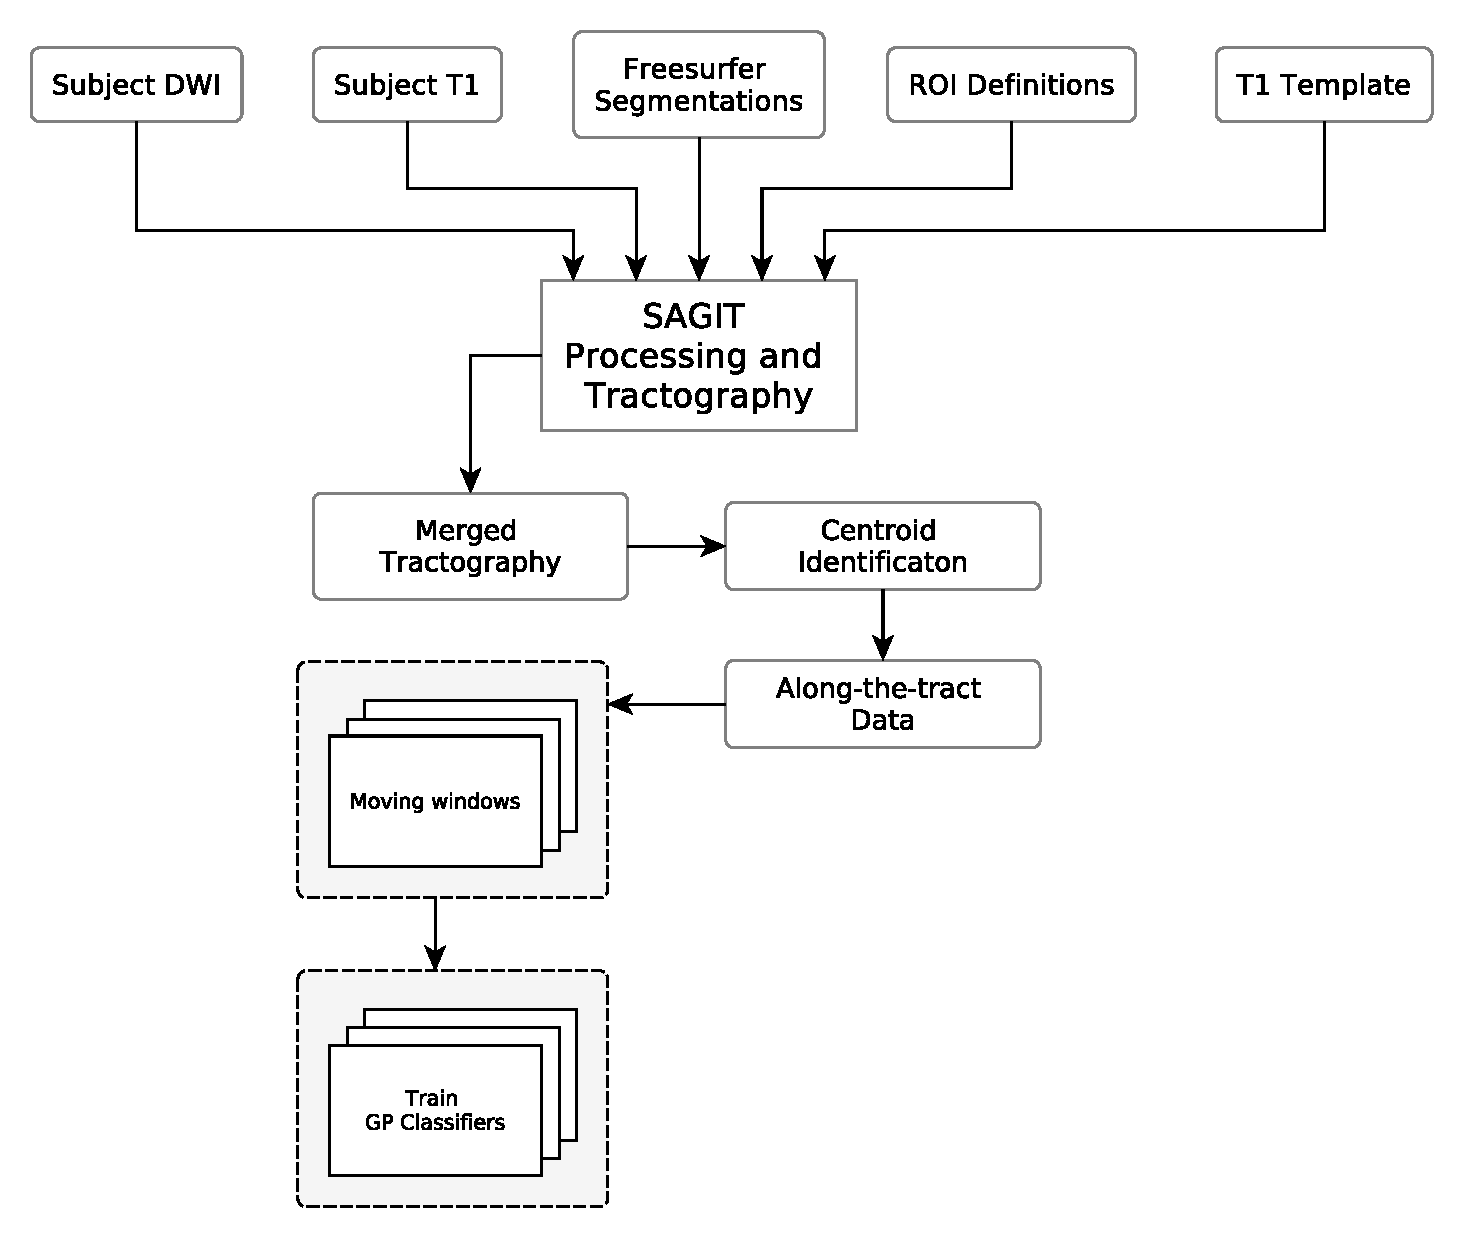
\includegraphics[width=\linewidth]{figure-method.pdf}
\caption{Diagram of the overall processing steps. The details of SAGIT processing steps can be found in \protect\cite{Chen2016}. Details of the centroid identification can be found in Figure \ref{fig:GPfigure-method-centroid}. The details for machine learning process can be found in Figure \ref{fig:GPfigure-gp-train}. }
\label{fig:GPMethods}
\end{figure}

\subsubsection{Acquisitions}
We studied 36 TN subjects with classic TN (28 females, 8 males; age 60.1$\pm$16.0 years; right sided pain), and 36 healthy controls (28 females, 8 males, age 42.7$\pm$12.0 years).  All TN subjects underwent non-invasive Gamma Knife radiosurgery, with imaging prior and six months post treatment. MRI acquisitions including T1 fast-spoiled gradient echo (FSPGR) and diffusion weighted image (DWI) acquisitions. 
T1 scans were acquired with 1mm slice thickness, in-plane resolution of 0.9375x0.9375 mm, with slice spacing = 1 mm, TE = 5.052 ms, TR = 11.956 ms, flip angle = $20^\circ$, FOV = 240 mm, and matrix = 256x256. 
DWI scans were acquired with 1 B0 scan, 60 gradient directions, 3 mm slice thickness and an in-plane resolution of 0.9375x0.9375 mm, where b0 = 1000 s/$mm^2$, TE = 88.6 ms, TR = 17000 ms, flip angle = $90^\circ$, field of view (FOV) = 120 mm, and matrix = 128x128.

\subsubsection{Preprocessing}
DWI images were motion/eddy-current corrected, with appropriate correction applied to the b-matrix \cite{Leemans2009}. ROI for tractography seeding were manually created on a normalized template brain from 42 healthy brains \cite{Chen2016}. The normalized brain template was created using Anatomical Normalization Tools \cite{Avants2010,Avants2011}. We deployed selective automatic group integrated tractography (SAGIT) framework \cite{Chen2016} to automate preprocessing, registration, and tract generation. The SAGIT processing steps are as follows: T1 anatomical images were processed using FreeSurfer \cite{Fischl2004} for cortical and subcortical segmentations. The T1 images for all the subjects were registered to the template using symmetric diffeomorphic registration (SDR) \cite{Avants2008b}. Each individual DWI was registered to their T1 image with SDR, using mean DWI image for DWI-T1 co-registration. Freesurfer segmentation maps were first affine transformed from the Freesurfer space to the T1 space using FMRIB's Linear Image Registration Tool (FLIRT) \cite{Jenkinson2001,Jenkinson2002}, and then transformed using SDR transforms to the individual DWI space for selective ROI generation with SAGIT.

\subsubsection{Tractography}
ROIs were defined on the template image to delineate the following bilateral structures: 1) CN V (specifications: ROI placed at cistern nerve root; excludes regions of cerebellum grey matter and pontine cerebellar peduncles); 2) trigeminothalamic pontine decussation (TPT) (ROIs placed at trigeminal nucleus (TGN); the fibers must traverse pontine decussation towards contralateral VC thalamus; pathway must exclude ipsilateral thalamus, cerebellar grey matter, pons, and contra-lateral S1 ); 3) thalamocortical S1 pathway (ROIs placed at VC thalamus; pathway must traverse the ipsilateral S1 white-matter boundary and exclude the brainstem).  

We used constrained spherical deconvolutional tractography (CST) \cite{Tournier2012b} to delineate the three defined anatomical regions. Deterministic and probabilistic streamline algorithms were used to delineate different regions, based on findings in the SAGIT study \cite{Chen2016}. Deterministic CST was applied to delineate CN V and S1 anatomy, while probabilistic (iFOD2) CST \cite{Jeurissen2011b,Tournier2010} was applied to delineate TPT anatomy. The parameters for each were as follows: Deterministic CST was performed with step size = 0.3 mm, angle threshold = $45^\circ$, streamline count = 200, minimal length = 5 mm, initial cut-off = 0.1, cut-off = 0.1, and with 4th-order Runge-Kutta integration. Probabilistic tractography for S1 projection was performed with step size = 5mm, angle threshold = $45^\circ$, streamline count = 300, max number of stream generation = 1 million, minimal length = 10 mm, maximum length = 80 mm, initial cut-off = 0.15, cut-off = 0.15. Probabilistic tractography for TPT project was performed with step size = 1 mm, and streamline count = 2000, and maximal length = 60 mm. Tractography was first performed in the native DWI space for each subject.  FA, AD, RD, MD, and GFA were embedded into the native tractography models by sampling the corresponding images maps using the points of the tractography geometry with tri-linear interpolation.

\subsubsection{Merged Tractography}
All tractography delineations of the same anatomy across all the subjects and groups were merged into a single tractography file for analysis. We have previously created a software library\footnote{https://github.com/sinkpoint/fascicle} to facilitate this process. Detailed steps are as follows: The individual tract files were converted into a SQLite relational database \cite{owens2010sqlite}, and  all points were exported and transformed by applying the subject DWI to T1, and T1 to template transforms using ANTS' applyTransformToPoints command \cite{Avants2009}. The transformed points were then imported back into the  database, and a new template-space tractography model is exported using the transformed point-set, with all its original scalars and subject/group associations preserved. Finally, all template-space tractography models across all the subjects are merged into a single file. 
The merged tract was post-processed in 3D Slicer to remove anatomically erroneous streamlines. These include remnant CN V streamlines that stray into the cerebellar peduncles or other non-TGN regions, and streamlines that are perpendicular to the nerve in the cisternal space that appear to be partial delineation of vessels or noise. TPT streamlines that did not decussate at the level of the pons, as well as fibers that stray into the contralateral TGN were removed. S1 streamlines that stray medially towards other regions such as the corpus callosum were also removed.

\subsubsection{Along-the-tract Analysis}
For the purpose of quantifying the trigeminal pathways, a centroid was defined for the merged tractography of each pathway (Figure \ref{fig:GPfigure-method-centroid}). The centroids were defined as the average curve that best fit the tract bundles and were in template space. CN V centroids were manually defined using 3 control points. A Catmull-Rom spline \cite{DeRose1988} was then defined from these control points using the VTK software library \cite{Schroeder2005}. The spline was then resampled into 30 subpoints. TPT and S1 centroids were defined using QuickBundles \cite{Garyfallidis2012} with distance threshold of 30. Nearest-neighbor point assignment was used to cluster the points of the merged tract model to the centroid subpoints, to obtain the corresponding 30 divisions along each centroid. Diffusion metrics from the tractography points were averaged for each of the divisions for each subject. 

\begin{figure}[ht]
\centering
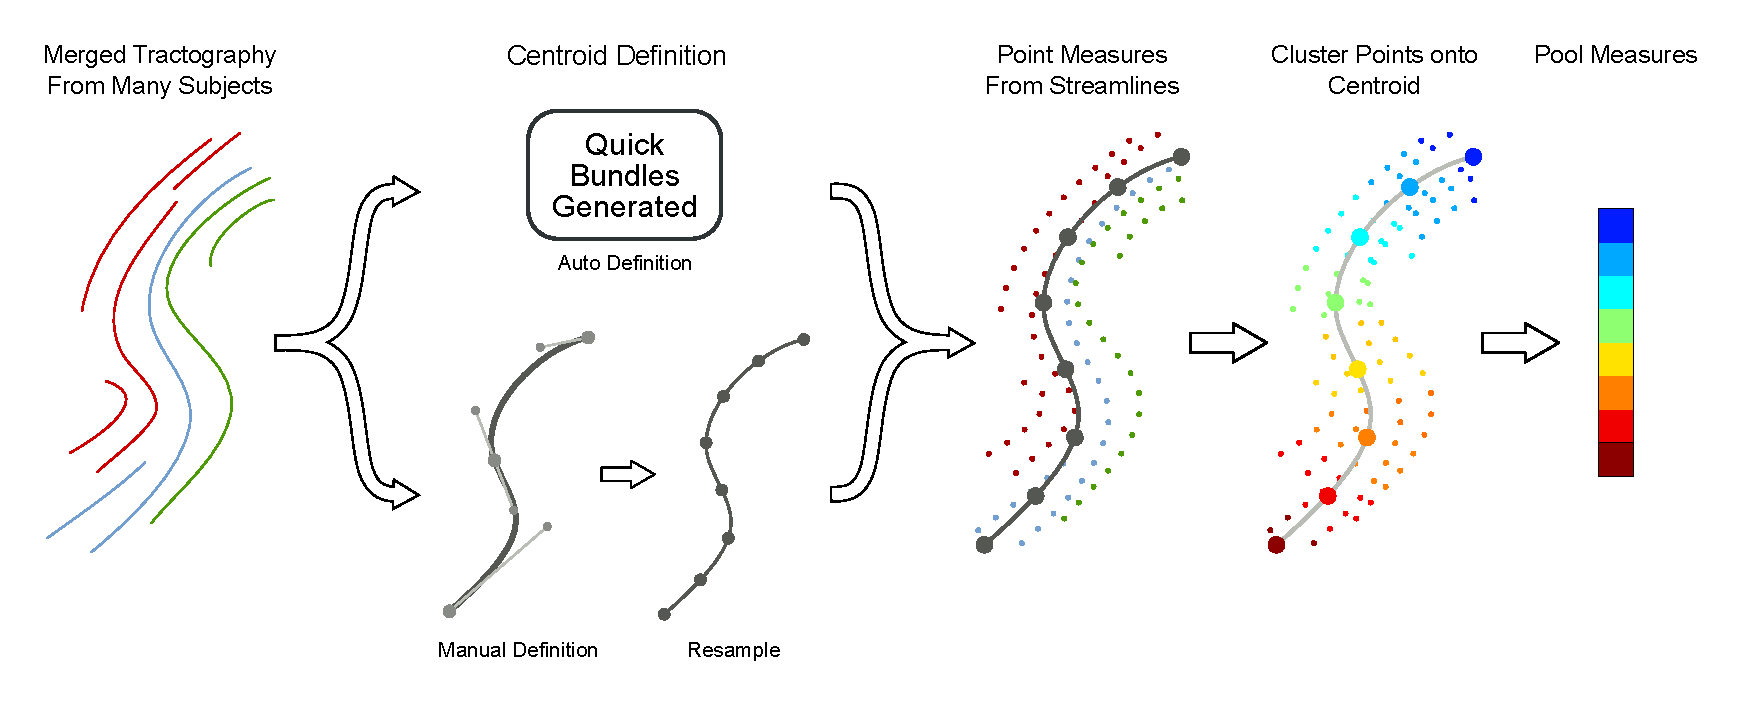
\includegraphics[width=\linewidth]{figure-path-analysis.pdf}
\caption{Diagram for the along-the-tract data processing.
Process starts with 2 specific goals: 1) Derive the spatial structure that best represent the merged streamlines, 2) Deriving sub-regional tissue information from these. A) First the best-fit curve is obtained to represent the collective streamlines, which is defined as the centroid. B) In areas where this can be automated, Quickbundles was used. For the CN V, the centroid was defined manually given the unpredictability of the lengths of streamlines. C) Representative drawing of the centroid onto the streamline points, representing the collective spatial information. The centroid is resampled to 30 subpoints. D) To derive tissue information, a nearest neighbor algorithm was used to assign streamline points to form 30 divisions. E) The average diffusivity metrics was pooled for each of the 36 subjects at each division. The colours represent the spatial position of each of the 30 divisions, and the streamline points that were assigned to each particular division. The data was then used for machine learning pipeline (see Figure \ref{fig:GPfigure-gp-train}).
}
\label{fig:GPfigure-method-centroid}
\end{figure}

\subsubsection{Gaussian Process Classification}

Diffusivity metrics of affected (right side) and unaffected CN V, TPT, and S1 pathways were independently compared with those of controls, where control metrics were the average of both left and right sides. The affected and unaffected sides in TN subjects were also compared with each other. 
Age was regressed out by using the residuals of the linear regression model from the controls group. The diffusion values were subsequently normalized to zero-mean with ranges $[-1, 1]$ for model training. 
Gaussian Process (GP) classification was performed to identify windows that resulted in the highest classification accuracies. Multiple moving windows of length between 5 to 30 were used to scroll through the centroid positions, and a Gaussian Process model was trained for each window (Figure \ref{fig:GPfigure-gp-train}). The machine learning process was performed using Scikit-learn machine learning software framework.
For each window, the subjects were split into train and validation sets using stratified 10-fold cross-validation, and a separate GP classifier was trained for each fold. GP models were initiated with Matern kernel (length scale = 1). The validation set was used to measure prediction accuracy, and the mean accuracy of the 10-fold cross-validation was used to assess the windows. Classification accuracy greater than 70\% were accepted, and the window with the greatest accuracy was then determined. 

\begin{figure}[ht]
\centering
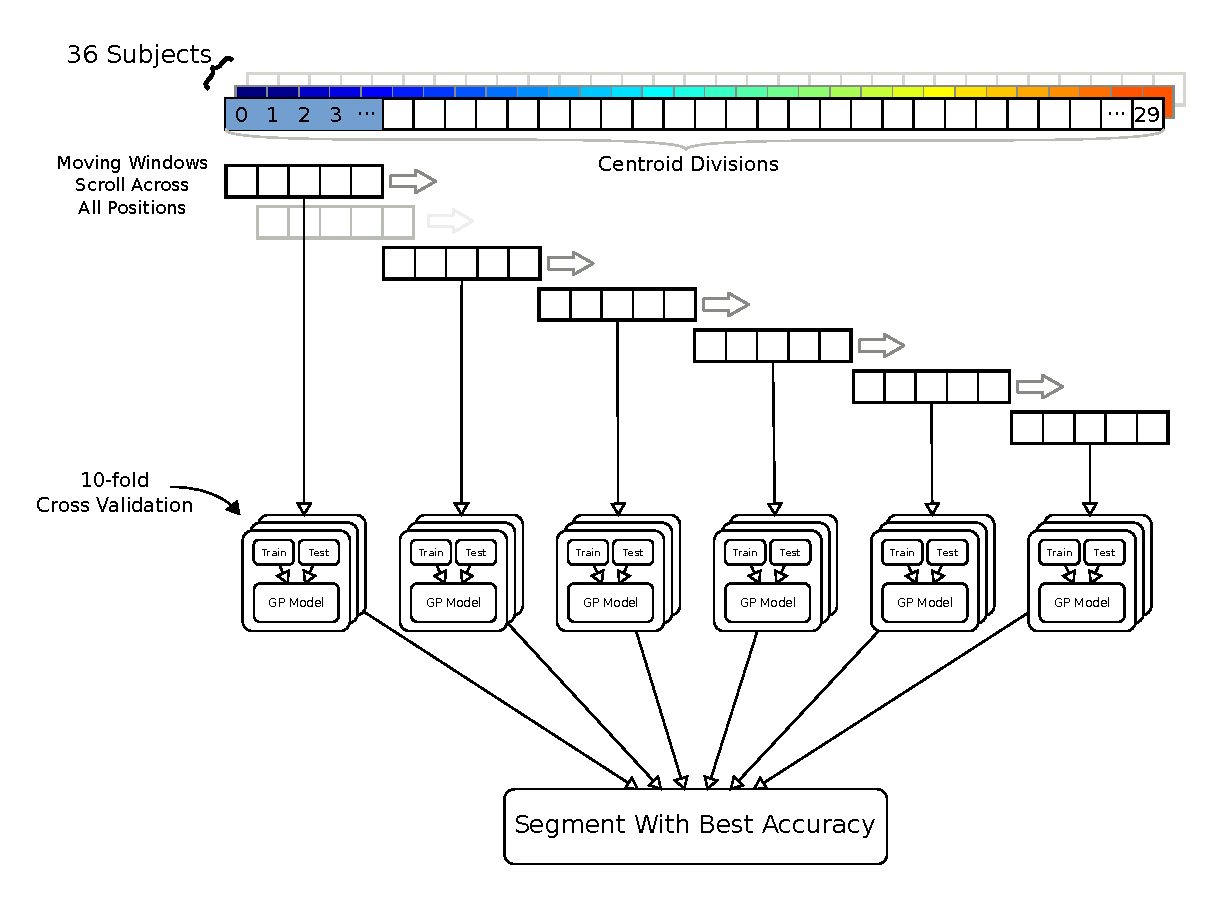
\includegraphics[width=\linewidth]{figure-GP-training.pdf}
\caption{Diagram for generating the best performing classifier for a particular window size. The data was derived from Figure \ref{fig:GPfigure-method-centroid}, where the top bar represents data from each centroid division, and each position represents the anatomical region of the trigeminal pathways within it. Each window was used to generate 10 GP models with 10-fold cross-validation, an average accuracy was determined at each window position. Finally the window position with the best accuracy was selected. The same process is repeated on every diffusivity metric, and for all window sizes ranging from 5 to 30. }
\label{fig:GPfigure-gp-train}
\end{figure}

\subsection{Results}
\subsubsection{Anatomical Delineations}
The findings in each of the three trigeminal areas are as follows: Merged CN V delineations show anatomical consistency from their position in the cisternal segment of the nerve and extending into the ipsilateral TGN. Changes in FA along the streamlines demonstrate clear step-wise increase at the interface between cistern and pontine segments, which is consistent with observations in single subjects. The FA metric of each point was sampled from the native DWI space of each subject, prior to the template space deformations. Therefore the sharp transition in FA in this anatomical landmark suggesting good agreement in the SAGIT anatomical registration (Figure \ref{fig:GPfigure1}). The CN V centroid curve length was determined as 38.91 mm, with the length of each subdivision being 1.3 mm.
The TPT projections from the TGN to the ipsilateral VC thalamus region showed distinct bundles of decussating pathways in both left and right projections. The resulting pathways were not symmetrical, where the right TPT pathway appears to divert around the left (Figure \ref{fig:GPfigure2}).
S1 streamlines reliably extended into the face region of the S1 cortex (Figure \ref{fig:GPfigure3}). The S1 centroid curve length was calculated to 62.1 mm and sub-division length was 2.07 mm.

\begin{figure}[ht]
\centering
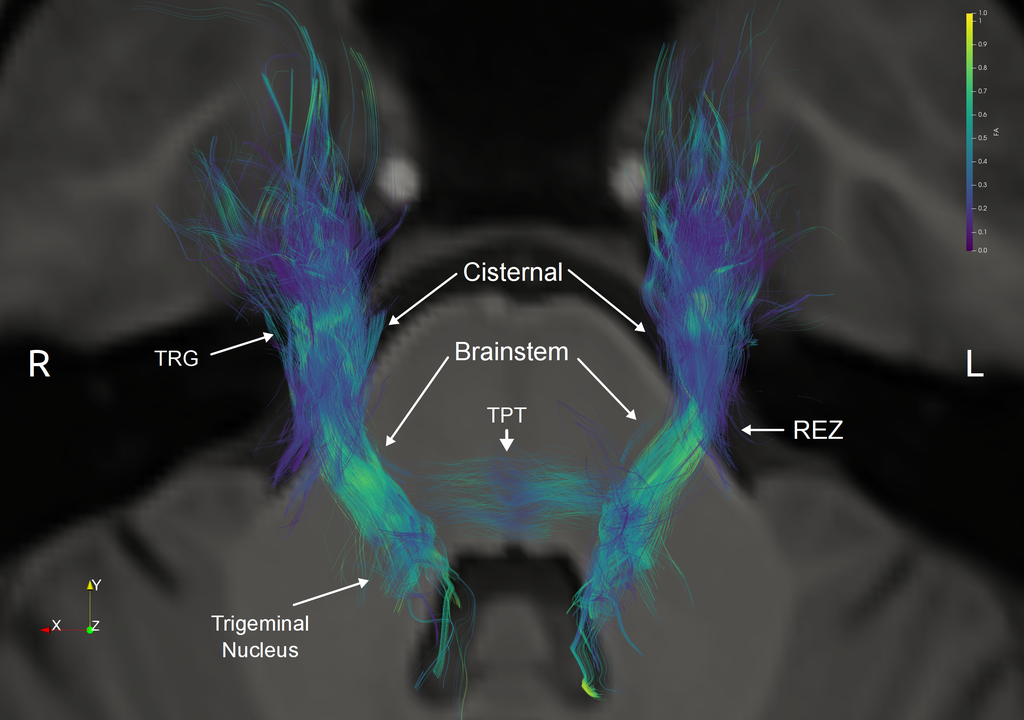
\includegraphics[width=\linewidth]{cnv-inferior-view-annotated.png}
\caption{Merged CN V reconstruction of 36 subjects, with the colour scale depicting FA values derived from raw streamlines, prior to the generation of centroids (see Figure \ref{fig:GPfigure-method-centroid} A). The expected increase in FA as the fibers enter the brainstem can be visualized, and denotes good registration between subjects. }
\label{fig:GPfigure1}
\end{figure}

\begin{figure}[ht]
\centering
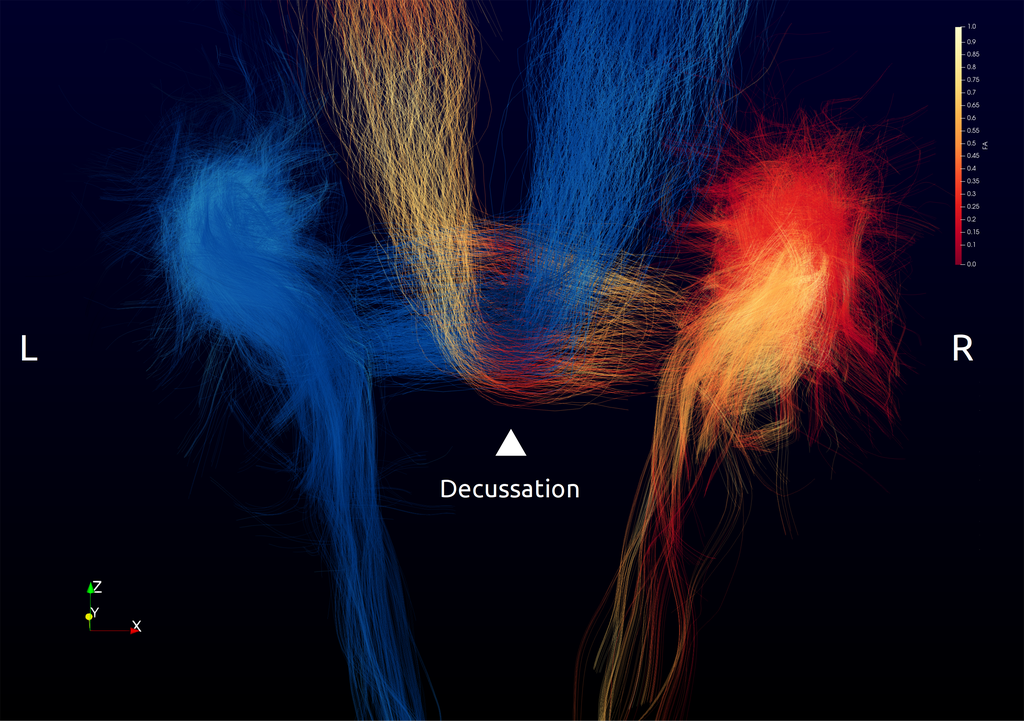
\includegraphics[width=\linewidth]{view-decussation.png}
\caption{Focused view of the TPT and its decussation, prior to the generation of centroids (see Figure \ref{fig:GPfigure-method-centroid} A). Colours were chosen arbitrarily to denote left and right pathways, however the colour intensity represents FA values as depicted by FA scale, top right corner. Red: Right TPT; Blue: Left TPT. Note the Right TPT appears to divert around the left TPT bundle. }
\label{fig:GPfigure2}
\end{figure}

\begin{figure}[ht]
\centering
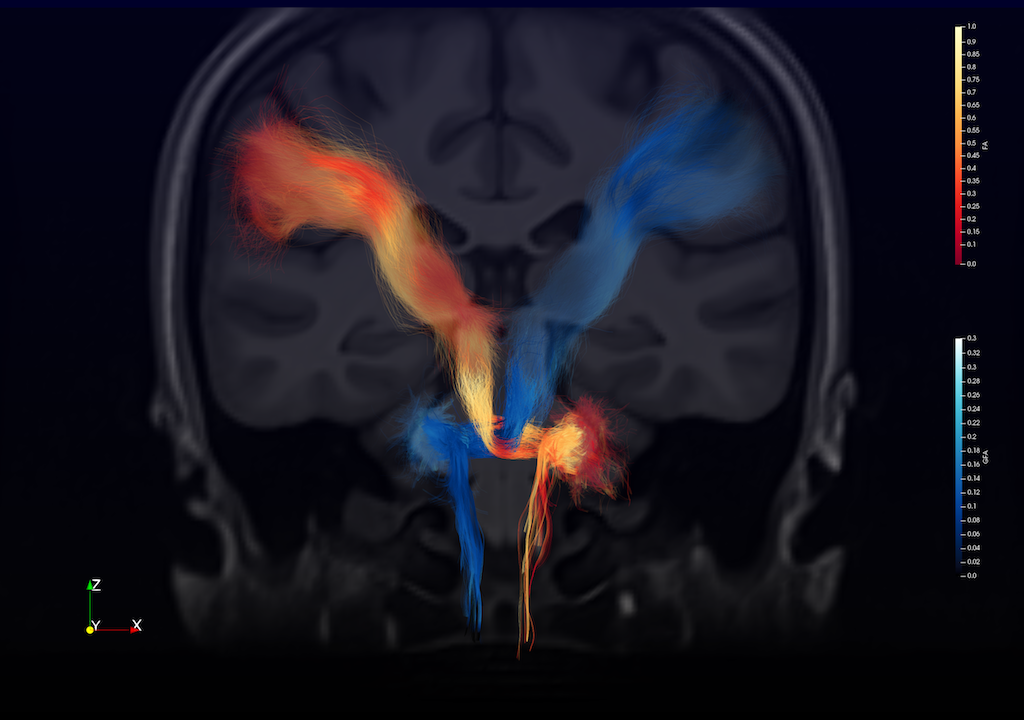
\includegraphics[width=\linewidth]{view-left-right.png}
\caption{Visual representation of the course of the trigeminal pathway from its cisternal component to the face area of the sensory S1 cortex. Images obtained prior to the generation of centroids (see Figure \ref{fig:GPfigure-method-centroid} A). FA is depicted by the colour intensities (Red: right side; Blue: left side). The trigeminal nerves, including the cisternal segments are seen in a coronal perspective (CN V), following which two pathways can be seen. The first pathway appears to head into the spine, while the second pathway consists of the TPT. Following the decussation, the fibers proceed to the area of the sensory thalamus and from there to the cortical sensory area S1.}
\label{fig:GPfigure3}
\end{figure}

\subsubsection{Diffusivity Differences}
\paragraph{CN V}
The classifier distinguished bilateral trigeminal nerves (affected and unaffected) from controls as well as affected trigeminal nerve from unaffected nerves. Both sides were distinguished from controls with classifiers that achieved near 80\% accuracy (Figure \ref{fig:GPfigure4}). 
Classifiers on the right (affected) side had accuracies ranging from 76\% (GFA) to 86\% (FA). The left (unaffected) classifiers achieved accuracy ranging from 79\% (MD) to 81\% (FA). The right side showed greater overlap of segment ranges between positions 14--24, which corresponds to the region of the cistern/ganglion; while the left side showed segments that covered the entire the nerve, and extended to cover position 0--4, within the substance of the trigeminal fibers in the brainstem. Overall, the windows of the right side classifiers extend further into the distal subdivisions, into the cistern and the area of the ganglion, while the left side extended more into the brainstem. FA classifier consistently achieved the highest accuracy in both sides, with right side at position 17--23 (cistern/ganglion) and left FA at 2--16 (brainstem/cistern).
The FA classifier achieved 75\% accuracy in differentiating affected versus unaffected nerves, where its segments ranged from 11 to 19, which was the cisternal segment. The GFA classifier achieved 70\% accuracy in region 9--12. Demonstrating that affected-unaffected diffusivity differences were found primarily in the cistern/REZ (Table \ref{table:GP}).

\begin{figure}[p]
\centering
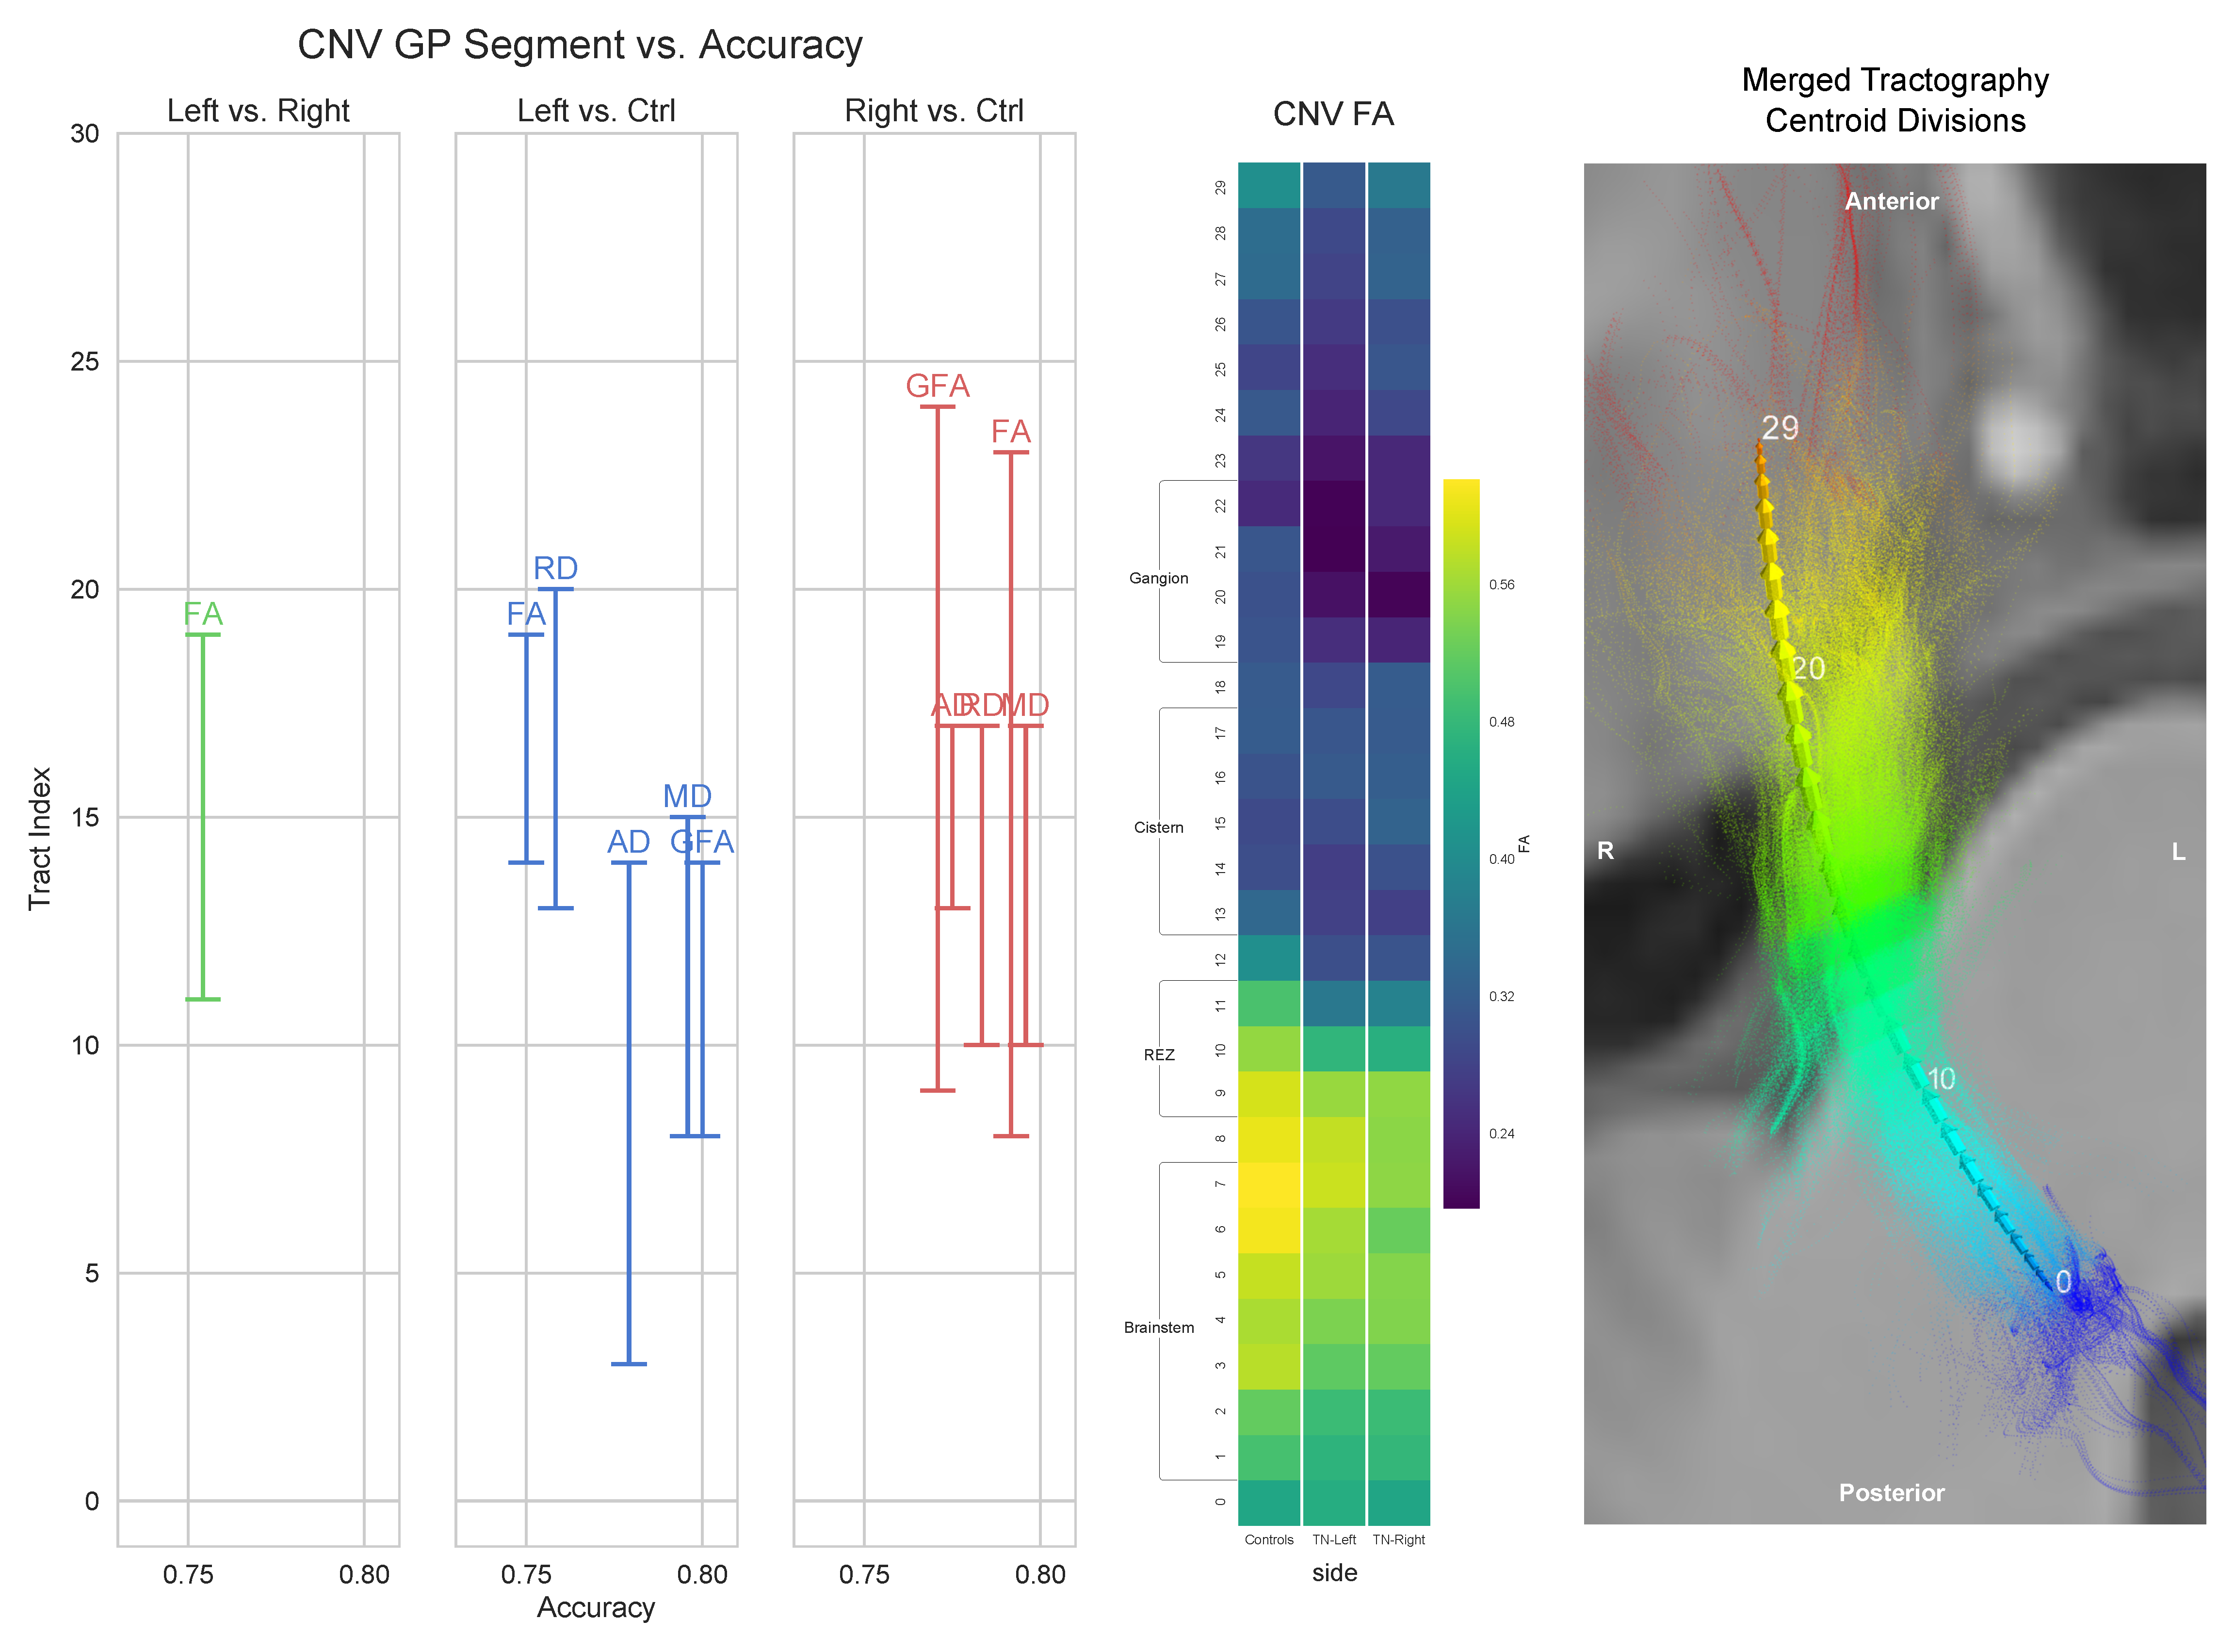
\includegraphics[width=1.2\textwidth,center]{figure-GP-CNV.pdf}
\caption{CN V classifier performances. This figure consists of 3 panels. Panel A, y axis represents the anatomical subregions of the trigeminal nerve as defined by the centroid subdivisions (see Figure \ref{fig:GPfigure-method-centroid}). Panel A, x-axis denotes the accuracy of the classifiers (scale of 0-1, with 1 representing 100\%)). Each diffusivity is denoted with respect to the window size (see Figure \ref{fig:GPfigure-method-centroid}) and position along the centroid where the accuracy is derived from. 3 instances are studied: comparison of left (unaffected) vs. control (average of both trigeminal nerves), comparison of right (affected) vs. control and comparison of left (unaffected) vs. right (affected). The colours for the diffusivity in each panel in A is arbitrary. Panel B is a heatmap (raw visualization) of FA values of the corresponding centroid positions. Panel C shows the centroid and point assignments for anatomical reference. The colours of the points correspond to their respective subdivision position as described in figure \ref{fig:GPfigure-method-centroid} and figure \ref{fig:GPfigure-method-centroid}} throughout the figure, the position of the centroid subdivisions are aligned and expressed with respect to the anatomical position as per panel B.
\label{fig:GPfigure4}
\end{figure}

\paragraph{Trigeminopontothalamic tract}
Classifiers could distinguish bilateral TPT pathways (affected and unaffected) from controls with greater than 80\% accuracy (Figure \ref{fig:GPfigureTPT}). The right (affected) FA classifier achieved the greatest accuracy at 85\% versus controls, and right RD classifier was least accuracy at 83\%. The left (unaffected) FA classifier showed greatest accuracy at 89\% and left RD classifier showed the least accuracy at 71\%. The classifiers covered both the decussation and the ascending segments of the TPT, with the right decussation showing more proximal coverage. The left-versus-right classifiers achieved maximum accuracy of 98\% (FA) and minimum of 88\% (MD). The FA classifier covered position 4--14, suggesting strong laterality differences in the TPT (Table \ref{table:GP}). 

\begin{figure}[ht]
\centering
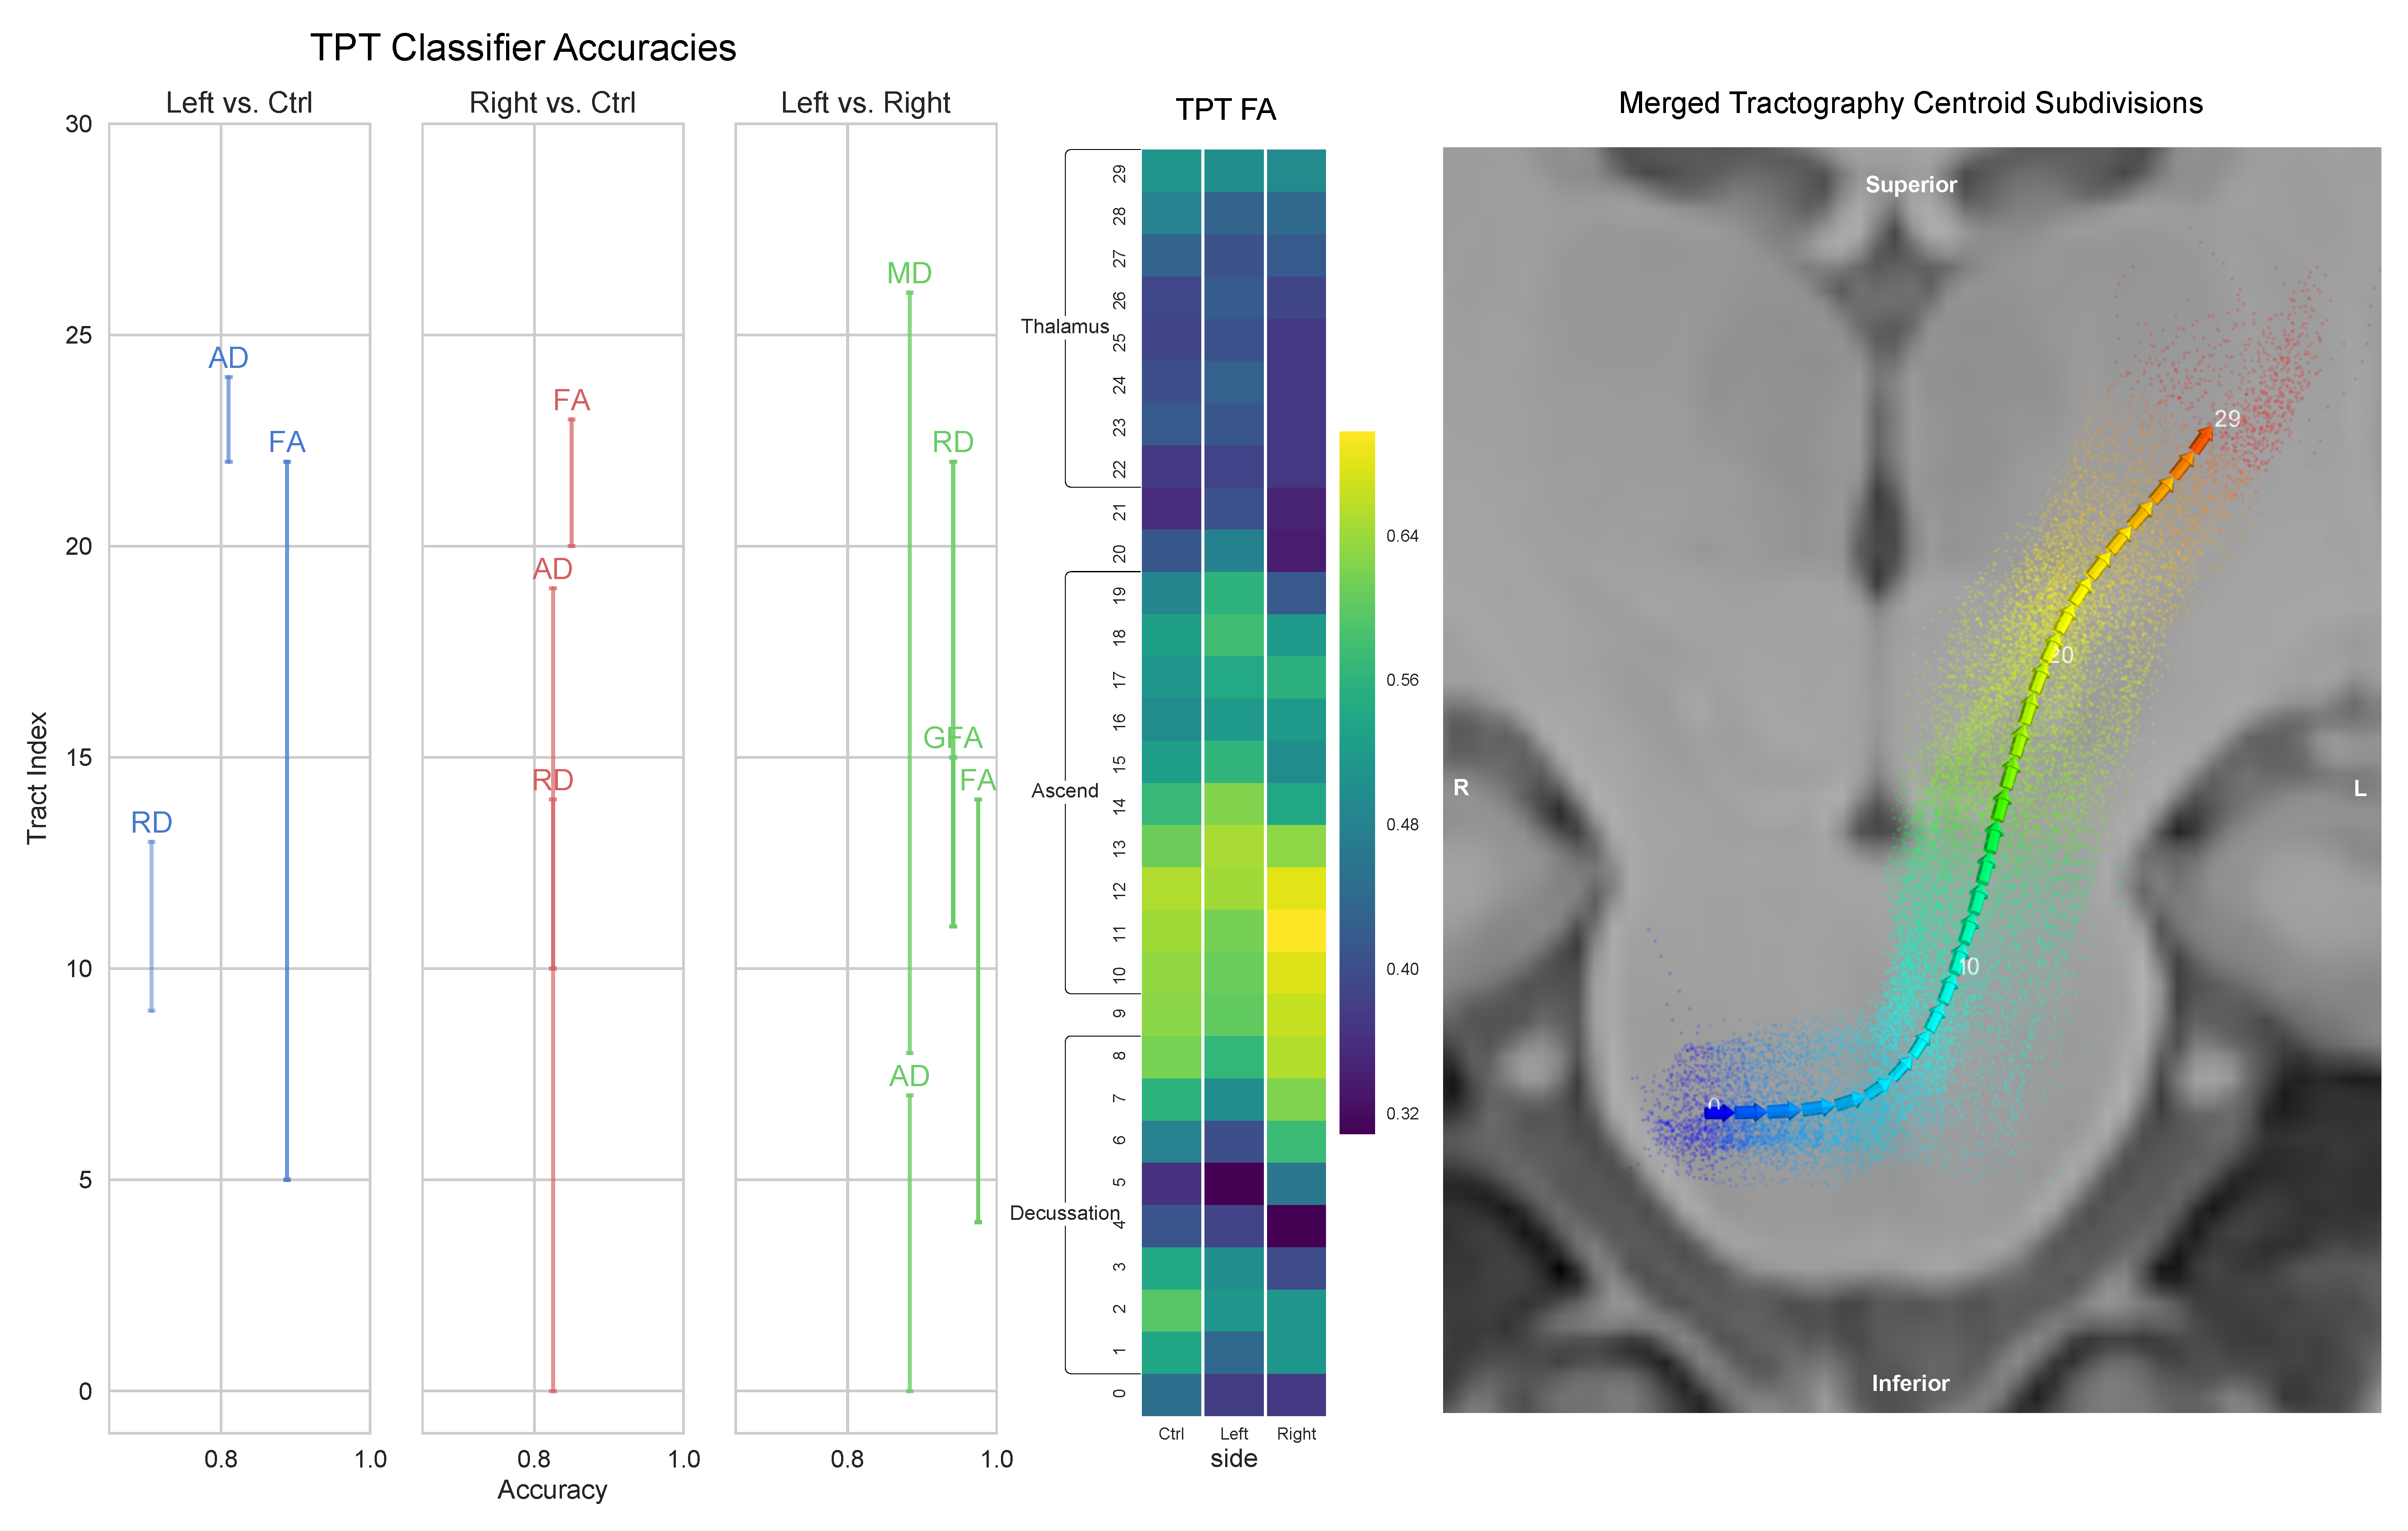
\includegraphics[width=1.2\textwidth,center]{figure-GP-TPT.pdf}
\caption{TPT classifier performance, see Figure \ref{fig:GPfigure4} for details on annotations.}
\label{fig:GPfigureTPT}
\end{figure}

\paragraph{S1}
Classifiers distinguished bilateral S1 face region pathways from controls with 85\% accuracy. The left (affected) RD classifier achieved maximal accuracy of 87\% at position 13--20, while the right (unaffected) RD classifier achieved maximal accuracy of 83\% at position 8--26 (Figure \ref{fig:GPfigure5}). Overall the left classifier ranged from 72\% (AD) to 87\% (RD), and the right classifiers ranged from 73\% (GFA) to 83\% (RD) (Table \ref{table:GP}). Classifiers of both sides covered the the branching region between the thalamus and cortex. Left-versus-right classifiers showed maximum accuracy of 78\% (RD), and minimum of 76\% (FA). The left-versus-right classifiers overlap in the regions 5--10, at the segment where the pathway emerges from the thalamus.

\begin{figure}[ht]
\centering
\includegraphics[width=1.2\textwidth,center]{figure-GP-S1.pdf}
\caption{S1 classifier performance, see Figure \ref{fig:GPfigure4} for details on annotations.}
\label{fig:GPfigure5}
\end{figure}

\begin{table}[p]
\centering
\small
\csvautotabular{tn_sagit_table.csv}
\caption{List of the best GP models for different diffusivity metrics and centroid windows. Only models with at least 70\% accuracy were accepted. Table is sorted by anatomical region, classifier type (R denotes right (affected) side versus controls; L denotes left (unaffected) side versus controls; LVR denotes left-versus-right ) and accuracy. Start and end denote the beginning and end of the window subdivision positions along the centroid. Length is the number of subdivisions covered by the window. Precision and f1 scores are provided for reference}
\label{table:GP}
\end{table}

\section{Discussion}
We have demonstrated the use of a fully-automated, end-to-end tractography and machine learning platform that is capable of discriminate TN from white-matter diffusivity with greater than 80\% accuracy strictly from white-matter measures. Our work is in agreement with previous findings of TN diffusivity changes along the CN V, yet the present technique offers much higher regional specificity, as well as examining the TPT and S1 projections of the trigeminal sensory pathway. The study is the first instance of machine learning discrimination of TN vs. controls with specific white matter analysis, using group-wise merged along-the-track tractography. 

The diffusivity measures of CN V agreed with our previous findings \cite{Chen2016a}, that the cistern, REZ differentiated TN from controls. The consistent regional overlaps in the cistern/ganglion region of the right (affected) CN V showed the ability for the GP classifiers to auto-converge to focal white-matter abnormality. The GP classifier placed affected vs unaffected differences at the cistern/REZ segment, in agreement with the pathophysiology of focal neurovascular compression in TN. 

The findings on unaffected (left) versus controls suggests bilateral differences in CN V diffusivities in unilateral TN, despite the lack of symptoms on the unaffected side. RD and AD have previously shown to relate to myelination \cite{Song2002} and axonal integrity \cite{Budde2009}. Therefore this finding is significant, since it suggests that the REZ and brainstem CN V ultrastructure might be bilaterally affected in unilateral TN pain, a process that may play important role in TN pain chronification, and responsiveness to surgery. The classifier windows of unaffected side also situate into the brainstem subdivisions. It is possible that the unaffected CN V is modulated by descending pathways \cite{Davis2013,Bushnell2013}. This point warrants further investigation.

The TPT left-verus-right FA/RD/GFA classifiers demonstrated very high accuracy (\textgreater 90\%), with overlapping windows in the ascending segment. The TPT merged tractography delineations showed that decussation pathway tractography is possibly asymmetric. The asymmetry of this decussation has not been demonstrated before. It is not clear whether this represents the anatomical arrangement of these fibers, or whether decussations are always purely symmetrical (akin to a perfectly shuffled deck of cards). Further assessment of other decussation points will be helpful to understand this process.  

We were able to successfully delineate the course of the fibers from the thalamus to S1 given the use of SAGIT and incorporation of Freesurfer cortical segmentation maps. Previous studies have suggested that S1 is involvement in pain location discrimination \cite{bushnell1999pain}, and have been found to exhibit grey-matter abnormalities in TN pain \cite{Desouza2013c}. We found that that while the left (affected) S1 RD classifier had higher accuracy (87\%) compare to the right S1 RD classifier (83\%), the left-verus-right classifier windows showed more overlap in subdivisions close to the thalamus. This suggests that while there is bilateral difference in the S1 pathways from controls, the difference between the segments mitigates as these reach closer to the S1 cortex.


The classifier windows showed a large variation of size. For example, amongst CN V classifiers (Figure \ref{fig:GPfigure3}), right MD consisted of 18 subdivisions, while right FA consisted of 7; The left classifiers showed a variety of sizes, yet the accuracy derived from each classifier were near 80\%. In the same manner, we observed variabilities in TPT and S1 classifiers window sizes. This suggests that classification according to a single diffusivity metric may be difficult to interpret, and thus multiple metric classifiers should be considered together. 

FA classifiers consistently achieved the highest accuracy in CNV and TPT, with the exception of S1. This might be due to the fact that it is known to have trouble in regions of heavy crossing-fibers. However, the TPT pathway also situations in regions of complex crossing fibers. One explanation for FA classifier in TPT is that the pathway courses through the narrow passage of pontine/thalamic regions, the fiber structures are highly constrained. Therefore FA still remains as a sensitive diffusivity metric for the TPT. 

We included GFA to investigate its potential for measuring cross-fiber white-matter diffusivity, as it is the most well-known non-Gaussian diffusivity metric. Although metrics such as FA are popular in current neuroimaging literature, they nevertheless are derived from the Gaussian tensor model, which cannot adequately describe cross-fiber regional dynamics. For example, in the crossing-fiber region of healthy tissue, where both bundles have equal myelin and axonal integrity, will have a low FA score due to a spherical tensor; its AD and RD will be roughly equal, and therefore MD will be higher. In a pathological cross region, where only one bundle is healthy, the FA increases due to the diffusivity bias in one direction; the RD will be lower, and MD will be lower as well. Moreover, in diverging and converging structures, as well as in multi-crossing regions such as the corona radiata, the interpretations of Gaussian-based diffusivity metrics become even more unclear. However results demonstrated that GFA did not perform to any substantially degree than the Gaussian-based diffusivity metrics such as FA. 

Overall the GP classifiers windows revealed areas in the TN pathways that would not have been captured using singular diffusivity metric analysis. Cross-metric features therefore should be considered in future studies. 

\subsubsection{Limitations}
The merged CN V delineations of all the subjects showed caudal projections towards the spinal cord. The consistent observation of diverging streamlines at the levels of the medulla strongly suggests that these fibers correspond to trigeminal spinal decussations. However the caudal projection were not consistently seen. This is likely due to the limited size of voxel resolution that in turn does not permit adequate resolution of medullary and spinal cord fiber details.

The DWI images were acquired at 0.9375$\times$0.9375$\times$3 $mm\textsuperscript{3}$ voxel resolution. The acquisition was a compromise to allow better in-plane resolution to image the trigeminal nerve, due to the limits of the 3T GE HDx MRI with 8-channels head coil. Our analysis is internally consistent, and SAGIT was previously validated on a identical sequence \cite{Chen2016,Chen2016a}, highlighting the validity of this approach. 

\subsection{Conclusions}
We have demonstrated group-wise along-the-track tractography machine learning analysis of TN vs. control. We have achieved the examination of specific and targeted anatomy at a group level involving both healthy and pathological brain images. The method agreed with previous findings of TN diffusivity changes along the CN V with finer-grained regional specificity. We also examined TPT and S1 projections of the trigeminal sensory pathway. The study revealed that there are specific diffusivity changes on these deeper white matter structures, and demonstrated the power of along-the-tract analysis with machine-learning, which pinpoints the exact location of the diffusivity disruption at millimetre level. 


\graphicspath{{images/discussions/}}

\chapter{General Discussions}

\section{Summary Of Findings}

The contribution of this thesis are as follows:

\begin{itemize}

\item Imaging of the brainstem segment of the CN V \textit{in vivo} using multi-tensor diffusion tractography. Prior to this work, CN V tractography was limited to single-tensor DTI models and trigeminal fibers could not be visualized as they enter into the pons. Clear delineation of the pontine CN V nerve allows reliable measurements of CN V diffusivity, therefore greatly increasing the range of study of trigeminal-related pathology that can be studied with neuroimaging, such as MS-TN. 

\item Differentiation between TN and MS-TN by examining sub-segment diffusivities, and distinguishing between cistern (TN) and brainstem peri-lesional (MS-TN) segments. This pathophysiological distinction between these two entities had not been previously demonstrated using neuroimaging tools, nor had it been correlated with the clinical expression of pain. 

\item Overcoming the major technical barriers to diffusion tractography study of the trigeminal pathway in a large population group, by developing and validating the Selective Automated Group Integrated Tractography (SAGIT) software platform. For the process, we determined the optimal T1-DWI co-registration methodology with clinical DWI sequences.

\item Merged group tractography study of the trigeminal nerve and its primary sensory pathway as a novel use of Gaussian Process machine learning to the study of TN. This study involved spatial defintion of groups tracts in space, as well as measurement of diffusivity metrics from the subregions of trigeminal primary (CN V), secondary (trigeminopontothalamic, TPT), and tertiary (thalamocortical, S1). We demonstrate distinct bilateral changes in trigeminal neuralgia subjects, as well as differences between affected and unaffected sides. 

\end{itemize}

\section{A new approach to the study of Trigeminal Neuralgia}


The introduction of DTI in the study of TN has revolutionized our understanding of this disorder. Moving away from clinical studies alone, DTI is able to derive metrics that provide important information on the microstructure of the nerve which can then be related to specific processes such as changes in myelination or the microstructure of the axons. Thus DTI provides an important objective measure in the study of pain, through a previously unavailable approach. The earliest work on the feasibility of accurate reconstruction of cranial nerve with DTI tractography \cite{Hodaie2010} dates to 2010. This study was able to image the optic nerve (CN II), oculomotor nerve (CN III), and importantly CN V. Similarly, we were able to establish the methods to image the trigeminal ganglion and the cisternal CN V with manual delineation, followed by visualization of the CN V area of radiosurgery target, prior and after treatment \cite{Hodaie2012g}. We found alternations in both the CN V reconstruction, as well as FA in the surgical target location, that improved our understanding beyond what is visible with post-surgical MRI gadolinium enhancements. This has now led our team to study whether CN V GK target diffusivity at 6 months post-surgery can predict long-term pain relief in TN \cite{Tohyama2018}, and similarly, whether the diffusivity changes are specific enough that they can serve as predictors of outcome \cite{Hung2017}. The tractography study of TN has been directly linked with the study of gray and white matter abnormalities of the TN brain \cite{Desouza2013c}. The value of DTI studies in TN is therefore unique, and creates a strong context for the work done in this thesis. 

The findings in Study I (Chapter \ref{section:study1}), point to the clear role of DTI in distinguishing the localized, focal changes in diffusivity that characterize TN and MS-TN. While TN is associated with compression of the REZ and possible associated focal central demyelination \cite{Devor2002a,Peker2006}, MS is associated with inflammation and myelin changes resulting in CNS plaques. While both diseases share a similar clinical expression of pain, the pathophysiology of pain differs, however this had not been shown directly using DTI based imaging techniques. From a technical perspective, the identification of the CN V nerve inside the brainstem from MR images had been previously highly inconsistent, and the precision of multiple ROI placements could not be maintained. Multi-tensor tractography was instrumental in the feasibility of the method. The study opened the possibility that multi-tensor tractography aided analysis added a measure of objective assessment in examining pain conditions, and may facilitate similar studies that provide insight into the fundamental changes that occur at the level of white matter. 

As a result of the methodology developed in Study I, a recent publication details the investigation of whether presurgical CN V segment diffusivity values can predict response to TN surgery \cite{Hung2017}. This important study found that lowered cistern MD and AD pre-surgery was correlated with positive surgical outcome, whereas lowered REZ FA and increased pontine AD was correlated with the lack of response from surgery. This provided further evidence of the role of cisternal CN V diffusivities in the study of TN. The fact that the novel finding of the role of pontine diffusivity in classic TN favours a non-responder outcome points to the role of CNS alterations in classic TN.

Study IV (Chapter \ref{section:study4}), applied group tractography to the study of the trigeminal sensory pathway, and highlighted the observation that the unaffected CN V diffusivity in TN differs significantly from that of controls. There have been other studies suggesting bilateral abnormalities in TN. A group level diffusivity study of TN was conducted by DeSouza et al. in 2013 \cite{Desouza2013} presented similar findings, with significant differences between affected and unaffected sides, but also between unaffected sides and controls. DeSouza manually defined the ROI in the trigeminal REZ, as well as performing full-brain Tract-Based Spatial Statistics. Bilateral differences in the REZ between TN patients and controls were found in MD, RD, and AD. Widespread white matter differences were also found, especially in the corpus callosum, cingulum, and longitudinal fasciculus.

Using SAGIT in study IV, the ROIs were projected to each individual subject using an automated pipeline. The GP classifier produced results by exhaustively examining moving windows at all position and sizes, and the results are auto-discovered by the algorithm, in contrast to manual-placement of the measurement ROI in previous studies. There is therefore consistency in CN V findings in the location and diffusivity across both manual and automated methods.

The observation of bilateral differences has important implications in our understanding of TN pain. From previous studies, it is clear that altered diffusivities in the cisternal and pontine segments of CN V are correlated with TN pain in the affected side. However, there are now a number of studies that point to bilateral REZ/pontine CN V diffusivities being altered in unilateral TN, although each point to significant differences between affected and unaffected sides as well. The exact nature of bilateral diffusivity alterations is not yet clear. Perhaps the earliest indication that TN can affect the nerves bilaterally is a clinical paper by the Burchiel group, where they point to a surprisingly large number of patients with unilateral TN that have evidence of bilateral neurovascular compression, in contrast with healthy controls \cite{Miller2009}. Moreover descending modulation from PAG can become maladaptive or ineffective in chronic pain, result in central changes in the trigeminal nucleus and its associated pathways.

Importantly, the unaffected side has been previously presumed to be similar to healthy controls due to the absence of pain. In many studies, it has also been used as a basis of comparison. With this additional insight, it becomes important to not interpret results of affected-to-unaffected comparisons in terms of differences between pathological and healthy tissue. Additionally, the logical next question is to determine that if the unaffected nerve differs from controls, at what point does the clinical expression of pain start. Investigations into bilateral TN pain, and vascular compression in the absence of pain, may reveal additional insight into the relationship between white matter changes and TN pain in general. The newly developed SAGIT and machine learning methods can additionally be leveraged to conduct large cohort studies, that allow investigation into the brain regions identified by DeSouza et al, as well as examining important areas in the modulation of pain, such as the insula and its relationship to TN. 

Finally, with the methods developed throughout this thesis, future studies are no longer restricted by manual ROI placements for each subject, and tract subregions can be studied in detail. This opens the avenue to the study of associated pathways of TN pain, and allow the development of more sophisticated prediction models to further the understanding, and treatment of TN. 

\section{Tractography of the trigeminal nerve and brainstem fibers}

An important motivation for the use of tractography to study the trigeminal nerve was the ability to overcome the significant limitations of current conventional MR imaging in the visualization of the brainstem trigeminal nerve and the area of the trigeminal nucleus. Prior to the use of tractography, the fibers of the trigeminal nerve and connected pathways could only be inferred from anatomical studies or postmortem dissections. 

The ability to resolve the pontine trigeminal nerve into the trigeminal nucleus signified that for the first time we could use software methods to segment the pontine trigeminal anatomy in a reliable manner. Prior to this, the ROI identification was done visually, and sometimes with simple heuristics methods based on distance from surrounding landmarks. Such manual methods were highly subjective and became problematic with the presence of pathology, where distortions to the nerve could not always be assessed. Improvements in tractography of the brainstem trigeminal nerve allowed the shift towards more algorithmic driven and automated segmentation and ROI placement.

Diffusion tensor imaging revolutionized how we examine brain white matter fibers, yet resolving cross-fibers of the cerebral white matter remains a limitation. The brain white matter consists of complex crossing fiber crossings, and the inability for DTI to reliably image these structure, therefore, poses a fundamental challenge for neuroimaging.
Techniques to improve visualization of white matter fibers consist of probabilistic tractography, which uses tissue priors to sample a large number of directions at each step stochastically, and combines the final result as a volumetric probability map. This kind of image-based probabilistic tractography has proved useful for whole-brain white matter studies. However, it is constrained to the resolution of the diffusion acquisition, which can be insufficient for localized and small diameter pathways. Moreover, the algorithm depends on pre-generated tissue-priors, which excludes cranial nerves. 
Deterministic algorithms such as diffusion spectral imaging (DSI), and the related multi-shell acquisition strategies attempt to model the fiber orientation distribution by dramatically increasing the number of gradient directions (256--512 directions where required) in the diffusion acquisition. The acquisition time of these sequences can be impractical for the clinical environment. Reduction in acquisition time for these algorithms is currently an active area of research.

The family of spherical harmonics (SH) based methods, which include Q-ball and constrained spherical deconvolution (CSD), are a significant development. SH-based methods model the fiber orientation distribution as a decomposition of SH basis functions. This means that these methods are more robust to noise, and therefore require less number of gradient acquisitions. CSD proved to be particularly robust to noise, and can be deployed on acquisitions with only 55 directions. Another family of tractography (XST) algorithm constrained its model assumption to two fiber crossings, also proved to provide good results with at least 50 gradient directions.

These algorithmic developments brought imaging of crossing-fibers using tractography to the realm of possibility. We explored the feasibility of imaging the pontine trigeminal nerve with CSD and XST. The trigeminal nerve is an ideal imaging target, both due to our immediate interest in TN, and also since the trigeminal nerve has a number of unique properties as a tractography target: 1) Its immediate morphology can be easily assessed in conventional MR images. 2) it courses through simple (cistern) and complex (pons) fiber environments; 3) it is a prominent cranial nerve, and therefore a good benchmark for imaging small anatomy.

For the purposes of imaging the trigeminal pathways, we divided the trigeminal nerve into 30 discrete cross-sections along its path, and observed detailed diffusivity changes as the nerve transitioned from pontine tissue to the cistern. The number of divisions chosen was arbitrary, with consideration that the number 30 could easily be divided into 3 sub-segments to represent the beginning, middle, and end of an elongated structure. In theory, the number of divisions could be infinitely large, given that a centroid curve was identified. Determining a common centroid curve from many subjects was computationally non-trivial, especially when the streamline lengths are variable. White matter pathways are highly complex, with possible multi-directional forks, bends, and convergent pathways across a wide range of scales. A generalized algorithm that can reliably calculate a centroid for these structures is of great value and yet still a topic of research. 
Merged tractography simplified this task by allowing a single curve to be defined manually in the template tractography space. This greatly simplified the task, since centroids no longer need to be separately defined  for each subject. Manually curve definition by experts can leverage known techniques in computer graphics to produce centroid for very complex structures, thereby extending SAGIT for obtaining along-the-track measure for other highly variable streamline bundles.

The segmentation of the subregions of the trigeminal pathway has allowed for the possibility of measuring the respective diffusivities. Moreover, this method can extend to any scalar images that can be registered to the DWI space. These may include specific tissue-metrics such as myelin and G-ratio images. This methodology is therefore highly applicable and not specific to the study of TN.


\section{Neuroimaging of deep white matter}

The findings relating to S1 in Study IV (Chapter \ref{section:study4}) showed TN diffusivity differences in regions surrounding the thalamus, as well as in the mid-segments of the S1 pathways. These findings were in agreement with previously published literature in this field, where thalamus and S1/S2 activations are often reported as part of the pain neuromatrix \cite{Melzack2008,Moayedi2012a}. The TPT pathway resulted in differences near the TGN and the thalamus, areas that are expected to be involved in TN pain. It would be of great interest to re-examine the MS-TN population in these pathways, in order to determine any relationship between deeper white-matter MS-lesion, MS-TN, and non-TN pain in the people with MS.

We have shown in Study III (Chapter \ref{section:study3}) that different tractography algorithms are suited to delineate different neuropathways when comparing merged reconstructions in 42 subjects. Maier-Hein et al came to similar conclusions after examining 96 reconstructions from a single set of simulated data \cite{Maier-Hein2017}. As tractography is applied to the investigation of white matter elsewhere in the brain, care must be taken to ensure parameters are targeted to the anatomy of study, as more consistent delineation leads to more robust tissue measurements.

Quantification of tissue measures from tractography, as demonstrated in Study IV, implies the use of points in tract models as a sampling method for the scalar values in DWI space. We demonstrated in Study III, that different tractography algorithms exhibit different geometric point distributions. In other words, given two tracts generated from identical ROI definitions, with similar cross-sectional area, but of different algorithm, the underlying spatial distribution of the points may be different. It can be argued that we average the point-metrics during along-the-tract analysis, which may be considered a form of smoothing/down-sampling, and therefore the spatial distribution of the tractography algorithm might not be as important. However, until the exact influence of spatial distribution have on the measured distribution of diffusivity metrics can be understood, comparing between similar tracts from two different tractography algorithms should be avoided.

\section{Machine Learning}


The availability of the SAGIT, full automation of tractography processing enabled a dramatic increase in the volume of data available for statistical analysis. This lead to some challenges in the scalability of the analytical process, but also opportunities in leveraging more expressive machine learning approaches. The need for data to improve diagnosis and treat of disease, particularly in the emergence of artificial intelligence in medical imaging is increasingly being recognized. Data is now the foundation from which new techniques and discoveries are possible. Initiatives such as the UK Biobank, Allen Brain Institute, and Ontario Brain Institute all collect and provide their neuroimaging data to researchers. With this deluge of imaging data, the complexity of analysis that demand of researchers proportionally increases. The need to include large amount of variables, patient attributes, study measures, time sequences, can now provide valuable insight that is beyond the mean of traditional statistics. In this thesis, we developed a machine learning approach that is scalable, and one that can quantify uncertainty as demanded by the medical need. The data processing and machine learning pipelineis end-to-end, meaning that the system can be practically deployed in a clinical setting.

We applied machine learning to the analysis of TN in Study IV. The analysis of the trigeminal nerve in TN versus controls agreed with our earlier findings, and therefore validates the study's GP classification method. Traditional multiple comparison statistical analysis in this setting becomes difficult to interpret.  We therefore decided that frequentist statistics was not suitable to our dataset, as we are burdened with too great amount of data, which may not fit with frequentist assumptions. 

The GP classifier was chosen over more popular SVM classifiers, for the following reasons: 1) the obtained metrics show high location dependency. 2) SVM results are hard to interpret, whereas GP is a Bayesian method, and therefore it is much more intuitive. More specifically, the streamline measurements resemble time-series data, in that it exhibits positional dependency between measurements. Unlike a time-series however, the streamline measurements represent physical locations along a pathway, therefore they exhibit bi-directional dependency, as opposed to uni-directionally dependent in time. Posing the study as a supervised machine learning problem, the feature vector would be an N-dimension vector representing N measures at each division, and a classification label. SVM would assume the features to be points in an N-dimensional space, and each measurement would assume independence. This makes the result of the SVM output difficult to interpret. The GP classifier models the feature vector as a latent GP model, before squashing it to produce a logistic output \cite{rasmussen2006gaussian}. Therefore the GP model is able to take the positional dependency into account. 
Changing the GP classification model into a regression one is relatively simple. This importance is illustrated thus: Study IV asked the question of at which measurement positions can we maximally discriminate TN from controls at a group level, but it is also possible to pose a prognosis question: Given N measurements along a single patient's CN V, what is the probability that the measurement distribution resembles a pathological population as opposed to a healthy population? It is possible to answer these questions trivially with the GP model using regression. The full implication is outside of the scope of this thesis, but this work will serve as a strong baseline for the applications in this direction. 




\section{Novel Technical developments}

\subsection{Delineating the brainstem fibers of the trigeminal nerve}

For successful tractography of the CN V, both DWI sequence and the algorithm choice are paramount. Given a DWI sequence, cisternal CN V could be readily reconstructed with Gaussian tensors. Unlike major white matter bundles, cranial nerves diameters are in the millimetre range, and therefore voxel sizes greater than 2 mm may result in partial volume averaging. Achieving 2 mm isovoxel on a 3T scanner requires a 32 channel head coil. Standard clinical 3T MRI scanners with 8 channels head coils can only achieve 2.6 mm isovoxel resolution before acquisition time and noise becomes insurmountable. For this reason, the acquisition in-plane resolution can be tuned to 1x1 mm, and slice thickness at 3mm. While the acquisition is not ideal, it sacrifices resolution only in the z-axis, however the tractography visual fidelity is improved. 
Imaging the brainstem CN V requires algorithms that can reliably resolve tract structures in regions with crossing fibers. A number of methods have been devised, including probabilistic tractography (FSL)\cite{Behrens2007}, which generates image-based results that represent the propagation probability of a seed region. Neurosurgical visualization however requires three dimensional representation of the fibers, and therefore streamline-based tractography visualizations are of broader appeal. In our experience, both XST and sphere harmonic based propagation algorithms can perform adequately to delineate brainstem CN V, as long as there are greater than 50 gradient directions. 

An important technical point consists in the tractography seeding pattern. When tracing the streamlines, an algorithm will need to generate a number of starting points in a defined volume. Common patterns in prepackaged software include in a regularly spaced grid and random sampling. The seeding pattern is important in both the final visual representation of the tracts, and to determine whether key anatomical landmarks can be properly tracked. Another consideration is the reproducibility of the desired anatomy, as randomly seeded bundles cannot be reproduced deterministically. Grid seeding may result in sparse spacing of the tract bundles when viewed from a certain angle, while random seeding can reduce this kind of visual artifact. A good balance might be to have a reproducible sampling scheme that also is robust to different viewing directions, for example a phyllotaxis pattern.

\subsection{Tractography group registration}
Tractography is a powerful methodology that permits the visualization of white matter fibers in three dimensions. Its primary use, however, has been limited to case studies and small-scale anatomy comparative analysis. The continuous advancements in big data and machine learning demand the adaptation of new neuroimaging methods to the analysis and quantification of larger groups.

Group comparative studies require the establishment of anatomical consensus, such that similar white matter structures between populations can be readily studied. Efforts in MRI medical image registration have paved the way to this end, especially in the fields of diffeomorphic registration. The difficulty in adapting registration to tractography is that tractography data has 3D geometry, and therefore is extremely difficult for analytical methods. To date, there are no direct non-linear 3D deformation methods for tractography. The best efforts to date apply affine transformation for between-tract registrations \cite{Garyfallidis2015}. Our approach is to recast tractography as a brain segmentation method while also making use of its orientation information. Thus tractography can be considered a point-based sub-sampling method that is represented in the same coordinate frame as the native DWI space. Any transforms applied to this DWI space is then applicable also to any tractography models that share its coordinate frame. Existing diffeomorphic registration solutions can then be used to non-linearly distort tractography, and circumvent the computational difficulty of geometry based non-linear registration. The advantage of our tractography registration strategy is that any new advances in the field of MR registration can be readily adapted to improve the output of our method. 

Group registration of tractography towards a common template space requires two separate steps: T1---DWI co-registration, and T1---Template registration. Any registration errors in these two steps will become multiplicative in the end result. T1 registration is well studied, however T1---DWI registration has limited literature. This demonstrates the need to investigate the best method to minimize registration errors that were compatible with our image data format.

\subsection{Measurements from tracts}
Aggregating along-the-measure statistics is a form of clustering that requires projection of tract vertices onto a structural skeleton, or centroid. Common clustering methods calculate a polyline centroid based on different distancing functions between streamlines. These methods require tractography streamlines to have similar length, and will underperform when tractography structures contain sharp turns. We have explored a number of strategies, and considered adaptation of manifold-based methods, and point-cloud skeletal extraction method from computer graphics literature. These approaches, however, contain assumptions that do not suit our needs. For example, manifolds commonly consider that the latent structure of the data lies on a lower-dimensional surface, while tractography is commonly arranged in complex bundles. Moreover, point-cloud methods deal with point-cloud data obtained from 3D scanners, which situate on a 3D shell, while tractography points are distributed within a volume. White matter anatomy can have intricate crossings, multi-way join and diverging structures. These are difficult for existing 3D analytical methods, and require models with simplified assumptions to reduce the number of unknown parameters. A potentially promising future direction may be to automatically discover these more complex latent structures using deep learning methods.

\section{Limitations}

One limitation across the studies in this thesis was the choice of anisotropic voxels of the DWI sequences. This was limited by the clinical 3-channel GE 3T HDx MR scanner, which places constraints both the acquisition resolution and time. Commonly, DWI voxel resolution on a 32-channel 3T research scanner can obtain up to 2mm isovoxel resolution, on older 8-channel clinical scanners, the maximum isovoxel resolution is limited at about 2.6mm isovoxel. This is insufficient for the study of cranial nerves such as CN V. Our resolution is limited to 1x1x3 mm voxel dimensions, in order to retain in-plane resolution at the sacrifice of slice thickness. Despite this, certain regions such as the TPT could not be reliably reconstructed in all of the subjects. Anatomy featuring intricate but complex cross-sections, such as the thalamoinsular projections which include the claustrum, and medullary decussations of the spinal trigeminal fibers will remain out of reach of the current algorithms without substantial improvement in DWI resolution. Fortunately, SAGIT can adopt MR images of any resolution, so future studies in higher isovoxel resolution can be immediately processed as soon as they become available. 

The results of the thesis ultimately depend on the algorithm performances at each step. The SAGIT framework relies on the accurate image registrations to perform template, and tractography deformations. Therefore any inaccuracies in the multi-step registration pipeline will become cumulative. We went to great length to determine the best method in order to minimize registration error on a massive scale (See \ref{section:study2}), and we stress the importance to strive for registration accuracy. 



\section{Future Directions}

The methods developed in this thesis, including SAGIT and merged-tractography GP classifiers, are not limited to the application to the study of TN. The methods can generalize to any white matter anatomy where consistent tracts can be obtained at a group level. The limitation of its examination power is often in the data, both in data volume, resolution, and quality.

Extensions to the current studies can follow three lines of investigations:

I) Advancing the limit of anatomical delineations towards other connections of the trigeminal system. This includes the spinal trigeminal pathways, which include the spinal trigeminal ganglion and its sub-ganglions, and its medullary decussations. Re-examine TPT tracts, both to establish its diffusivity baseline, and to confirm its asymmetry. Image the medial pain pathways, and descending projections to the PAG. These tasks are currently limited by the resolution of available DWI images. Immediate gains may be obtained by using SAGIT to delineate these structure on the Human Connectome Project (HCP) dataset. Additionally, investigation into 7T DWI images will be necessary. 

II) Re-examine TN and other pain in the MS population with S1/S2 and TPT pathways. The localization ability of merged-tractography analysis can be readily applied to white-matter lesion studies, and may reveal additional insights in the MS population, where focal lesion groups can be correlated with disease symptoms such as pain and motor disabilities. Comparative studies with other trigeminal pain syndromes such as post herpetic neuralgia and trigeminal deafferentation pain would be a valuable direction.

III) Continue to advance machine learning to enable disease diagnosis and prognosis from white-matter tractography. Investigate how to diagnose and provide treatment targets from MR images with minimal turn around time. This can involve applying GP regression to the prediction of patient disease, and multi-modal learning, possibly with deep neural networks. Gaussian Process can be used as a regressor to model tissue parameters along merged white-matter bundles. Any MR scalar image can be embedded into the tractography streamlines, so tissue quantifications such as G-ratio, myelin, proton-density, kurtosis, magnetization transer, PET images can be examined. Since GP is a Bayesian method, the derived GP model can be used to provide predictive confidence on centroid measures from single subjects. When combined with the end-to-end tractography extraction ability of SAGIT, this provides a basis to build a deployable framework for disease inference on new patients. 


We observed that merged tractography could delineate more complete pathways than any single subject. This is similar to the observation that averaged MRI anatomical images from multiple subjects can produce high-quality templates. Therefore merged tractography may serve to produce high-quality tractography templates, that can form the basis for both geometric and measurement comparisons in individuals. We have explored the use of SAGIT in generating the first neonatal porcine tractography template \cite{Zhong2016a}. Such template does not exist for humans to the best of our knowledge, and can be readily created from Human Connectome Project data. In patients where tractography cannot be reliably delineated, for example in the case of severe white matter degeneration in MS or low-resolution clinical acquisitions, these template tracts may provide a standard population distribution for GP regression, and can be used as a proxy to enable advanced analysis.

The pain neuromatrix, as studied by various functional and structural connectivity studies, distributes over the full range of neocortical areas. These areas are associated with complex white-matter pathways that extend to all regions of the brain. These include sharp curvatures of the anterior pain pathways of the ACC, the distant projections of the temporal cortices. Some pathways are just beyond the feasibility of current methods. These include the projections of the insula and claustrum, small descending pathways to PAG, and the spinal trigeminal pathways in the brainstem. Detailed examination of the pain matrix with the inclusion of these pathways, such as the medial pain-related white matter projections of the ACC, and posterior insula would be of great interest. Multi-modal and multi-variable study with functional connectivity with this technique would also be possible. 

Tractography, in conjunction with 3D anatomical segmentation, can 1) reconstruct white matter pathways that are otherwise difficult to visualize directly, and 2) allow intuitive spatial relationship of key anatomies that are hard to visualize in 2D. We had previously demonstrated these capabilities in the reconstruction of deformed facial/vestibular nerve complex in relation to vestibular schwannomas \cite{Chen2011b,Behan2017}.
Another contribution is to visualize tissue changes from surgical interventions. There are cases where post-operative GammaKnife ablation target on the trigeminal nerve did not result in discernible gadolinium enhancement in standard MR, but the nerve FA changes can be seen in the delineated tractography. Therefore tractography can provide both spatial, as well as tissue-based insights to the surgeons to aid in assessment.
Tractography and 3D anatomical model ultimately are standard 3D geometries in computer graphics. Therefore advances in 3D printing can be easily adopted in neurosurgery to allow surgeons to physically examine tractography reconstructions. On the other hand, technologies such as virtual reality (VR) and augmented reality (AR), which are simply different ways to present computer graphics, can allow new ways to empower surgeons in decision making. Tractography can play a key role in bridging computer vision based diagnosis and surgical disease intervention to improve surgical outcomes and improved quality-of-life for patients.   

\section{Conclusions}

In sum, this thesis provides novel evidence on the diffusivity tissue disruptions of the CN V in TN, and that there is evidence of bilateral CN V tissue changes in TN patients when compared to controls. The examination was also extended to the thalamocortical S1 pathway and have demonstrated localized white matter changes near the white-grey matter boundary. These examinations on the group level were made possible by the development of the SAGIT merged tractography framework, that can be generally applied to group-based white matter studies as a whole. These results demonstrate that TN involves wide-spread changes at all levels of CNS white matter, and that the methods developed in this thesis may lead to improvements in white matter disease detection and diagnosis.

%\backmatter
% bibliography, glossary and index would go here.
%\addcontentsline{toc}{chapter}{Bibliography}

\bibliographystyle{apacite}
\bibliography{mendeley,external_refs}

\end{document}